\documentclass[11pt, twoside]{article}
\usepackage[paperwidth=165mm,paperheight=235mm, textwidth=360pt, textheight=541.40024pt, inner = 25mm, outer = 15mm]{geometry}

\usepackage[width=181mm, height=251mm, cam, center]{crop}
\def\longer{22.7621}
\def\shorter{14.2263}
\newcommand*\cropa{%
	\begin{picture}(0,0)
		\thinlines\unitlength1pt
		\put(-\longer,0){\line(1,0){\shorter}}
		\put(0, \longer){\line(0,-1){\shorter}}
	\end{picture}%
}
\newcommand*\cropb{%
	\begin{picture}(0,0)
		\thinlines\unitlength1pt
		\put(\longer,0){\line(-1,0){\shorter}}
		\put(0,\longer){\line(0,-1){\shorter}}
	\end{picture}%
}
\newcommand*\cropc{%
	\begin{picture}(0,0)
		\thinlines\unitlength1pt
		\put(-\longer,0){\line(1,0){\shorter}}
		\put(0,-\longer){\line(0,1){\shorter}}
	\end{picture}%
}
\newcommand*\cropd{%
	\begin{picture}(0,0)
		\thinlines\unitlength1pt
		\put(\longer,0){\line(-1,0){\shorter}}
		\put(0,-\longer){\line(0,1){\shorter}}
	\end{picture}%
}
\cropdef[]\cropa\cropb\cropc\cropd{cam_new}
\crop[cam_new]

\usepackage[cmyk]{xcolor} % PDF needs to be in CMYK colour space for printing
\usepackage{../problem-collection-book}

\begin{document}

\begin{titlepage}
	\centering
	\vspace{10cm}
	{\sffamily\Huge \mbox{200 EESTI FÜÜSIKAOLÜMPIAADI}\\ ÜLESANNET AASTATEST\\ 2005 -- 2011\par}
	\vspace{1cm}
	{\Large koos vihjete ja lahendustega\par}
	\vfill
	{\Large Koostas Taavet Kalda}

	\vfill

	% Bottom of the page
	{\large 2019}
\end{titlepage}

\raggedbottom % Because of twosided
\mbox{}\vfill

\textcopyright~Autoriõigused: Eesti Matemaatika Selts, Tallinna Tehnikaülikool,
Tartu Ülikool, ülesannete autorid ja Taavet Kalda.
\vspace{0.5\baselineskip}

Kogumiku koostamist toetasid: Eesti Matemaatika Seltsi fond ``Benoit Mandelbroti Jälgedes'', Robert Kitt ja Tallinna Tehnikaülikool.
\vspace{0.5\baselineskip}


Korrektor ???

Kaanekujundaja Rael Kalda

Saatesõna Robert Kitt ja Jaan Kalda
\vspace{0.5\baselineskip}

Kirjastanud Tallinna Tehnikaülikooli eelõppeosakond
\vspace{0.5\baselineskip}

ISBN ???
\newpage

\tableofcontents
\newpage

{\setlength{\parindent}{24pt}
\section{Sissejuhatus}

Siia on koondatud 200 gümnaasiumi ülesannet Eesti füüsikaolümpiaadi piirkonnavoorudest, lõppvoorudest ja lahtistest võistlustest. Igale ülesandele on juurde kirjutatud paarilauseline vihje. Juhul kui õpilane jääb ülesannet lahendades toppama, on tal võimalik vihjet lugeda ning teisele katsele minna.

Tegu on teise kogumikuga Eesti füüsikaolümpiaadi ülesannete kogude seerias, kus esimene kattis 200 ülesannet ajavahemikust 2012---2018.

Ülesanded on jaotatud teemade kaupa ning teemasiseselt raskuse järgi. Raskustaset tähistatakse kuni viie tärniga. Ülesannete lihtsamaks otsimiseks on ülesannete numbrite ette pandud \enquote{Ü}, vihjete ette \enquote{V} ja lahenduste ette \enquote{L}. Näiteks ülesande 133 teksti number on kujul Ü133. Iga ülesande juures on kirjas ka selle autor ning olümpiaadi vooru lühinimetus, lisaks lühendid P 1, G 1 jne, kus tähed tähistavad põhikooli- ja gümnaasiumiastet. Näiteks G 9 viitab gümnaasiumiastme 9. ülesandele.

Kogumiku koostamise käigus eemaldati erinevatel põhjustel 3 ülesannet.
\newpage
\setlength{\parindent}{0pt}

        \section{Ülesanded}
        \ToggleStatement
        \subsection{\protect\StrSubstitute{Dünaamika}{-}{ }}

\graphicspath{{../problems/}}

% Ü1
\ylDisplay{Kivi} % Ülesande nimi
{Aigar Vaigu} % Autor
{lõppvoor} % Voor
{2005} % Aasta
{G 1} % Ülesande nr.
{1} % Raskustase
{
% Teema: Dünaamika
\ifStatement
Sirgjooneliselt ja jääva kiirusega $v = \SI{4}{m/s}$ tõusva õhupalli gondlis asub poiss. Mingil hetkel laseb poiss gondlist alla kukkuda kivi ning seejärel viskab ta kivile järgi palli, soovides tabada palliga langevat kivi. Milline võib olla suurim ajavahemik kivi lahtilaskmise ja palli viskamise vahel, et see oleks veel võimalik? Maapinnal seistes suudaks poiss visata palli vertikaalselt üles kuni $h = \SI{20}{m}$ kõrgusele. Võib eeldada, et õhupall asub piisavalt kõrgel selleks, et kivi saaks palliga tabada enne maapinnale kukkumist. Õhutakistus lugeda tühiseks. Raskuskiirendus $g = \SI{9,8}{m/s^2}$.
\fi
}

% Ü2
\ylDisplay{Pallid} % Ülesande nimi
{Tundmatu autor} % Autor
{lahtine} % Voor
{2007} % Aasta
{G 1} % Ülesande nr.
{1} % Raskustase
{
% Teema: Dünaamika
\ifStatement
Juku istub puu otsas ja laseb algkiiruseta lahti tema käes oleva palli. All seisab Juhan, kes samal hetkel viskab vertikaalselt üles täpselt samasuguse palli Juku pihta. Pärast pallide põrget jõuab Juku pall täpselt tema kõrgusele tagasi. Kas pall tabab Juhanit enne või pärast seda, kui Juku pall jõuab Jukuni? Lugeda, et pallide põrge on absoluutselt elastne.
\fi
}

% Ü3
\ylDisplay{Hobune} % Ülesande nimi
{Valter Kiisk} % Autor
{piirkonnavoor} % Voor
{2007} % Aasta
{G 1} % Ülesande nr.
{1} % Raskustase
{
% Teema: Dünaamika
\ifStatement
Puu oksal istub poiss, kes soovib hüpata puu alt mööda galopeeriva hobuse selga. Hobuse kiirus on $v = \SI{10}{m/s}$ ja puuoksa kõrgus sadula suhtes $h = \SI{3}{m}$. Kui suur peab olema horisontaalsihiline distants sadula ja puuoksa vahel sel hetkel kui poiss oksast lahti laseb?
\fi
}

% Ü4
\ylDisplay{Eiffeli torn} % Ülesande nimi
{Aigar Vaigu} % Autor
{piirkonnavoor} % Voor
{2010} % Aasta
{G 1} % Ülesande nr.
{1} % Raskustase
{
% Teema: Dünaamika
\ifStatement
Eiffeli torni ülemiselt vaateplatvormilt (kõrgus maapinnast
$h=\SI{273}{m}$) lastakse kukkuda raudkuul. Täpselt $t=3$ sekundi pärast kukutatakse
veel üks raudkuul. Kui suur on raudkuulide suurim
kiiruste vahe langemisel? Kui suur on ajavahemik kuulide maapinnale jõudmiste
vahel? Raskuskiirendus $g=\SI{9.8}{m/s^2}$. Katse käigus ükski külastaja viga ei saanud.
\fi
}

% Ü5
\ylDisplay{Kokkupõrge} % Ülesande nimi
{Andreas Valdmann} % Autor
{piirkonnavoor} % Voor
{2011} % Aasta
{G 1} % Ülesande nr.
{1} % Raskustase
{
% Teema: Dünaamika
\ifStatement
Kaks autot massidega $m=\SI{1,5}{}$ tonni teevad laupkokkupõrke, mille võib lugeda täielikult plastseks. Kui suur energia kulus purustuste tekitamiseks, kui:\\
\osa mõlema auto kiirus oli $v_a=\SI{50}{\kilo\metre\per\hour}$; \\
\osa üks auto seisis paigal ja teise auto kiirus oli $v_b=\SI{100}{\kilo\metre\per\hour}$?\\
(Võib arvestada, et autode lohisemisel pärast põrget olulist kahju ei teki.)
\fi
}

% Ü6
\ylDisplay{Tõus} % Ülesande nimi
{Tundmatu autor} % Autor
{lahtine} % Voor
{2005} % Aasta
{G 2} % Ülesande nr.
{2} % Raskustase
{
% Teema: Dünaamika
\ifStatement
Talvise ilmaga Tartust Tallinnasse sõitev auto peab oma teekonna alguses ületama järsu ja libeda tõusu Jakobi tänaval (vt joonist). Tõusu kallak horisontaalsihi suhtes $\alpha \approx \SI{5}{\degree}$, pikkus $l \approx \SI{200}{m}$. Hinnata, kui suur on minimaalne hõõrdetegur $\mu$ rataste ja tee vahel, mille puhul kiirusega $v = \SI{30}{km/h}$ mäkke üles sõitma hakkanud auto suudab veel tõusu ületada?

\begin{center}
	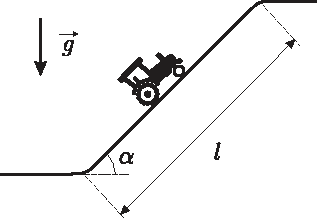
\includegraphics[width=0.5\linewidth]{2005-lahg-02-yl}
\end{center}
\fi
}

% Ü7
\ylDisplay{Keha} % Ülesande nimi
{Tundmatu autor} % Autor
{lahtine} % Voor
{2006} % Aasta
{G 3} % Ülesande nr.
{2} % Raskustase
{
% Teema: Dünaamika
\ifStatement
Vertikaalselt ülesse visatud keha läbib kaks korda kõrgusel $h$ asuvat punkti. Ajavahemik nende kahe läbimiste vahel on $\Delta t$. Leida keha algkiirus $v_0$ ja aeg $\tau$ keha liikumise algusest kuni algpunkti tagasi jõudmiseni.
\fi
}

% Ü8
\ylDisplay{Mootorratas} % Ülesande nimi
{Tundmatu autor} % Autor
{lahtine} % Voor
{2007} % Aasta
{G 5} % Ülesande nr.
{2} % Raskustase
{
% Teema: Dünaamika
\ifStatement
Mootorrattur tahab hüpata üle kraavi, mille mõõtmed on näidatud joonisel. Kui suur peab olema mootorratturi minimaalne kiirus $v$ lennu alguses selleks, et tema ettevõtmine õnnestuks?

\begin{center}
	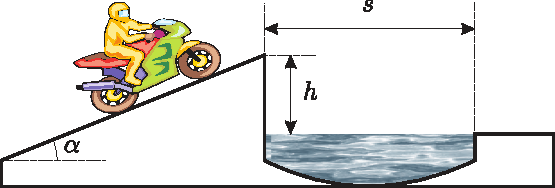
\includegraphics[width=0.8\linewidth]{2007-lahg-05-yl}
\end{center}
\fi
}
\newpage


% Ü9
\ylDisplay{Kelk} % Ülesande nimi
{Tundmatu autor} % Autor
{lahtine} % Voor
{2008} % Aasta
{G 2} % Ülesande nr.
{2} % Raskustase
{
% Teema: Dünaamika
\ifStatement
\begin{wrapfigure}[5]{r}{0.4\textwidth}
	\begin{center}
		\vspace{-20pt}
		\hspace{-10pt}
		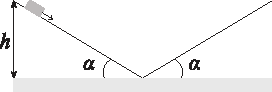
\includegraphics[width=\linewidth]{2008-lahg-02-yl}
	\end{center}
\end{wrapfigure}
Kelguga lastakse alla $h = \SI{10}{m}$ kõrgusest $\alpha = \SI{30}{\degree}$ kaldenurgaga orunõlvast. Kui kõrgele tõuseb kelk saadud hooga mööda sama suure kaldenurgaga vastasnõlva, kui hõõrdetegur on $\mu = \num{0,1}$? 

\emph{Märkus}. joonis on ligikaudne, languselt tõusule üleminek on tegelikult sujuv ja põrkega seotud kiirusekadu seal ei toimu.
\fi
}

% Ü10
\ylDisplay{Hantel} % Ülesande nimi
{Mihkel Kree} % Autor
{lõppvoor} % Voor
{2008} % Aasta
{G 1} % Ülesande nr.
{2} % Raskustase
{
% Teema: Dünaamika
\ifStatement
Hantel koosneb kahest võrdse massiga kerast (kumbki massiga $m$) ning neid ühendavast massitust jäigast vardast. Alguses hoitakse hantel horisontaalselt õhus paigal. Nüüd antakse ühele kuulidest hetkega vertikaalsuunaline kiirus $v$ ning hantel hakkab vabalt liikuma. Vabalangemise kiirendus on $g$. Missugune on süsteemi kineetiline energia hetkel, mil massikese saavutab maksimaalse kõrguse?
\fi
}

% Ü11
\ylDisplay{Ping-pong} % Ülesande nimi
{Siim Ainsaar} % Autor
{lõppvoor} % Voor
{2008} % Aasta
{G 2} % Ülesande nr.
{2} % Raskustase
{
% Teema: Dünaamika
\ifStatement
Pingpongipall kukutatakse kõrguselt $h$ horisontaalsele lauale. Igal põrkel kahaneb palli energia $k$ korda. Leidke palli lahtilaskmisest seismajäämiseni kuluv aeg $t$. Vabalangemise kiirendus on $g$.
\fi
}

% Ü12
\ylDisplay{Mürsk} % Ülesande nimi
{Mihkel Kree} % Autor
{piirkonnavoor} % Voor
{2009} % Aasta
{G 2} % Ülesande nr.
{2} % Raskustase
{
% Teema: Dünaamika
\ifStatement
Kahurist välja lennanud mürsk (massiga $M$) laguneb oma lennutrajektoori kõrgeimas punktis mingi sisemise vedrumehanismi abil kaheks võrdseks pooleks (kumbki massiga $M/2$) nii, et üks osadest kukub mürsu senist trajektoori pidi liikudes täpselt kahurini tagasi. Kui kaugele kahurist maandub teine pool? Lagunemispunkti projektsioon maapinnale asub kahurist kaugusel $L$.
\fi
}

% Ü13
\ylDisplay{Kerad} % Ülesande nimi
{Valter Kiisk} % Autor
{lahtine} % Voor
{2010} % Aasta
{G 1} % Ülesande nr.
{2} % Raskustase
{
% Teema: Dünaamika
\ifStatement
On antud kolm väliselt identset ja ühesuguse massiga kera. On teada, et üks
neist keradest on homogeenne, teine on seest õõnes ja kolmas on seest vedel.
Kuidas saab lihtsate võrdlevate mehaanikakatsetega kindlaks teha, milline on iga
kera sisemus? Abivahendid võite vabalt valida, aga kerasid vigastada ei tohi.
\fi
}

% Ü14
\ylDisplay{Sild} % Ülesande nimi
{Valter Kiisk} % Autor
{lõppvoor} % Voor
{2010} % Aasta
{G 1} % Ülesande nr.
{2} % Raskustase
{
% Teema: Dünaamika
\ifStatement
Risti üle $l=\SI{100}{m}$ laiuse jõe kulgeb kumer sild, mille keskel on
autotee $h=\SI{5}{m}$ võrra kõrgemal kaldapealsest tasemest. Silla profiiliks on
ringjoone kaar. Auto massiga $m=\SI{1000}{kg}$ ületab silla muutumatu kiirusega $v=\SI{60}{km/h}$.
Kui suure jõuga rõhub auto silla keskkohta? Kui suure kiiruse juures hakkab kaduma
kontakt rataste ja tee vahel?
\fi
}

% Ü15
\ylDisplay{Varras} % Ülesande nimi
{Stanislav Zavjalov} % Autor
{lõppvoor} % Voor
{2011} % Aasta
{G 2} % Ülesande nr.
{2} % Raskustase
{
% Teema: Dünaamika
\ifStatement
Mööda liigendi abil seina külge kinnitatud väga pikka ja tühiselt
kerget varrast saab libiseda väike rõngas massiga $m$. Esialgu asub rõngas liigendist kaugusel $l$ ja varras on horisontaalne. Ajahetkel $t = \num{0}$ hakkab süsteem
vabalt liikuma. Leidke varda ja horisontaali vahelise nurga $\alpha$ ajaline sõltuvus.
Kõik liikumised lugeda hõõrdevabaks. 
\fi
}

% Ü16
\ylDisplay{Karatist} % Ülesande nimi
{Tundmatu autor} % Autor
{lahtine} % Voor
{2007} % Aasta
{G 6} % Ülesande nr.
{3} % Raskustase
{
% Teema: Dünaamika
\ifStatement
Hinnake, millise kiirusega $v$ peab karatisti käsi tabama kahele kivile toetuva lauajupi keskpunkti (vt joonist), et laud murduks? Käe mass on $m = \SI{1,5}{kg}$, laua mass $M = \SI{2}{kg}$, laua jäikustegur $k = \SI{1,4e5}{N/m}$, murdumiseks vajalik läbipaine (st laua keskpunkti nihe) $d = \SI{20}{mm}$. 

\emph{Märkus}. Jäikustegur $k$ on võrdetegur laua keskpunkti rakendatud jõu $F$ ning laua keskpunkti nihke $x$ vahel (vt joonist).

\begin{center}
	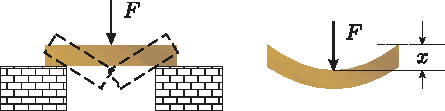
\includegraphics[width=0.8\linewidth]{2007-lahg-06-yl}
\end{center}
\fi
}

% Ü17
\ylDisplay{Veenus} % Ülesande nimi
{Mihkel Kree} % Autor
{lõppvoor} % Voor
{2007} % Aasta
{G 2} % Ülesande nr.
{3} % Raskustase
{
% Teema: Dünaamika
\ifStatement
Lugegem Maa ja Veenuse orbiidid ümber Päikese ringikujulisteks. Planeedid tiirlevad ümber Päikese samas suunas ja Veenuse maksimaalne eemaldumus (nurk Veenuse ja Päikese vahel Maalt vaadates) on 46 kraadi.\\
\osa Leidke Veenuse ja Maa orbiitide raadiuste suhe.\\
\osa Mitu päeva jääb järjestikuste maksimaalsete eemaldumuste vahele?

\emph{Vihje}. Kepleri seaduse kohaselt on taevakehade tiirlemisperioodide ruudud võrdelised vastavate orbiitide raadiuste kuupidega.
\fi
}

% Ü18
\ylDisplay{Auto} % Ülesande nimi
{Mihkel Heidelberg} % Autor
{piirkonnavoor} % Voor
{2009} % Aasta
{G 5} % Ülesande nr.
{3} % Raskustase
{
% Teema: Dünaamika
\ifStatement
Auto kiirendab nii, et rattad libisevad. Hetkel on auto kiirus stabiilselt $v$, vedavate rataste nurkkiirus $\omega$ ja raadius $r$. Kui oletada, et mootori võimsus läheb ainult auto liikumisse ja vedavate rataste libisemisse, siis kui suur on kasutegur?
\fi
}

% Ü19
\ylDisplay{Vedru} % Ülesande nimi
{Aigar Vaigu} % Autor
{piirkonnavoor} % Voor
{2010} % Aasta
{G 4} % Ülesande nr.
{3} % Raskustase
{
% Teema: Dünaamika
\ifStatement
Raske tellis kukub poole meetri kõrguselt jäigale lühikesele vedrule. Põrge
on elastne ja tellis lendab peaaegu algsele kõrgusele tagasi. Kui
kõrgele maast kerkib vedru pärast põrget?
\fi
}

% Ü20
\ylDisplay{Pendel} % Ülesande nimi
{Taavi Pungas} % Autor
{piirkonnavoor} % Voor
{2011} % Aasta
{G 7} % Ülesande nr.
{3} % Raskustase
{
% Teema: Dünaamika
\ifStatement
Pendel pandi väikese amplituudiga võnkuma ning stopperiga registreeriti neid hetki, kui pendel läbis vasakult poolt tulles oma tasakaalupunkti. Kaks järjestikust sellist sündmust toimusid hetkedel $t_1=\SI{3,19}{s}$ ja $t_2=\SI{5,64}{s}$. Pendlil lasti mõnda aega segamatult võnkuda, seejärel saadi kaheks järjestikuseks näiduks $t_3=\SI{61,14}{s}$ ja $t_4=\SI{63,54}{s}$. Leidke võimalikult täpselt pendli võnkeperiood ning hinnata selle mõõtemääramatust.
\fi
}

% Ü21
\ylDisplay{Aerud} % Ülesande nimi
{Tundmatu autor} % Autor
{piirkonnavoor} % Voor
{2005} % Aasta
{G 6} % Ülesande nr.
{4} % Raskustase
{
% Teema: Dünaamika
\ifStatement
Aerude pikkus tullist (punktist, kus aerud kinnituvad paadi kere külge) kuni käepidemeni on $a = \SI{1}{m}$ ning tullist kuni labadeni on $b = \SI{1,5}{m}$. Keskmine jõud, millega aerutaja tõmbab kumbagi aeru, on $F = \SI{60}{N}$. Paadi ja vee vaheline takistusjõud on $F_h = \alpha v^2$, kus $\alpha = \SI{20}{kg/m}$. Kui suure keskmise kiirusega liigub paat? Hinnata aerutaja keskmist võimsust.
\fi
}

% Ü22
\ylDisplay{Kivi} % Ülesande nimi
{Tundmatu autor} % Autor
{lahtine} % Voor
{2006} % Aasta
{G 4} % Ülesande nr.
{4} % Raskustase
{
% Teema: Dünaamika
\ifStatement
Paelaga lae külge kinnitatud kivi liigub mööda horisontaaltasapinnas asuvat ringjoont, mille kaugus laest $h = \SI{1,25}{m}$. Leida kivi tiirlemisperiood $\tau$. 
\fi
}

% Ü23
\ylDisplay{Kaldpind} % Ülesande nimi
{Mihkel Rähn} % Autor
{piirkonnavoor} % Voor
{2006} % Aasta
{G 4} % Ülesande nr.
{4} % Raskustase
{
% Teema: Dünaamika
\ifStatement
Pall kukub kaldpinnale ja hakkab elastselt põrkuma (st energiakadudeta). Kui kaugel on viies põrkekoht esimesest? Kaldpinna kaldenurk on $\alpha$, palli algkõrgus esimesest põrkekohast oli $h$.
\fi
}

% Ü24
\ylDisplay{Kuulike} % Ülesande nimi
{Tundmatu autor} % Autor
{lahtine} % Voor
{2008} % Aasta
{G 5} % Ülesande nr.
{4} % Raskustase
{
% Teema: Dünaamika
\ifStatement
Venimatu ja kaalutu niidi otsa kinnitati kuulike.
Niit viidi horisontaalasendisse ja lasti lahti. Kuulikese kiiruse vertikaalne komponent
hakkab esialgu suurenema, kuid teatud hetkest alates vähenema. Millise nurga moodustab niit vertikaalsihiga ajahetkel, kui kuulikese kiiruse vertikaalne komponent on
maksimaalne?
\fi
}

% Ü25
\ylDisplay{Veerev silinder} % Ülesande nimi
{Andres Laan} % Autor
{lahtine} % Voor
{2010} % Aasta
{G 3} % Ülesande nr.
{4} % Raskustase
{
% Teema: Dünaamika
\ifStatement
\begin{wrapfigure}[7]{r}{0.3\textwidth}
	\vspace{-10pt}
	\hspace{-8pt}
	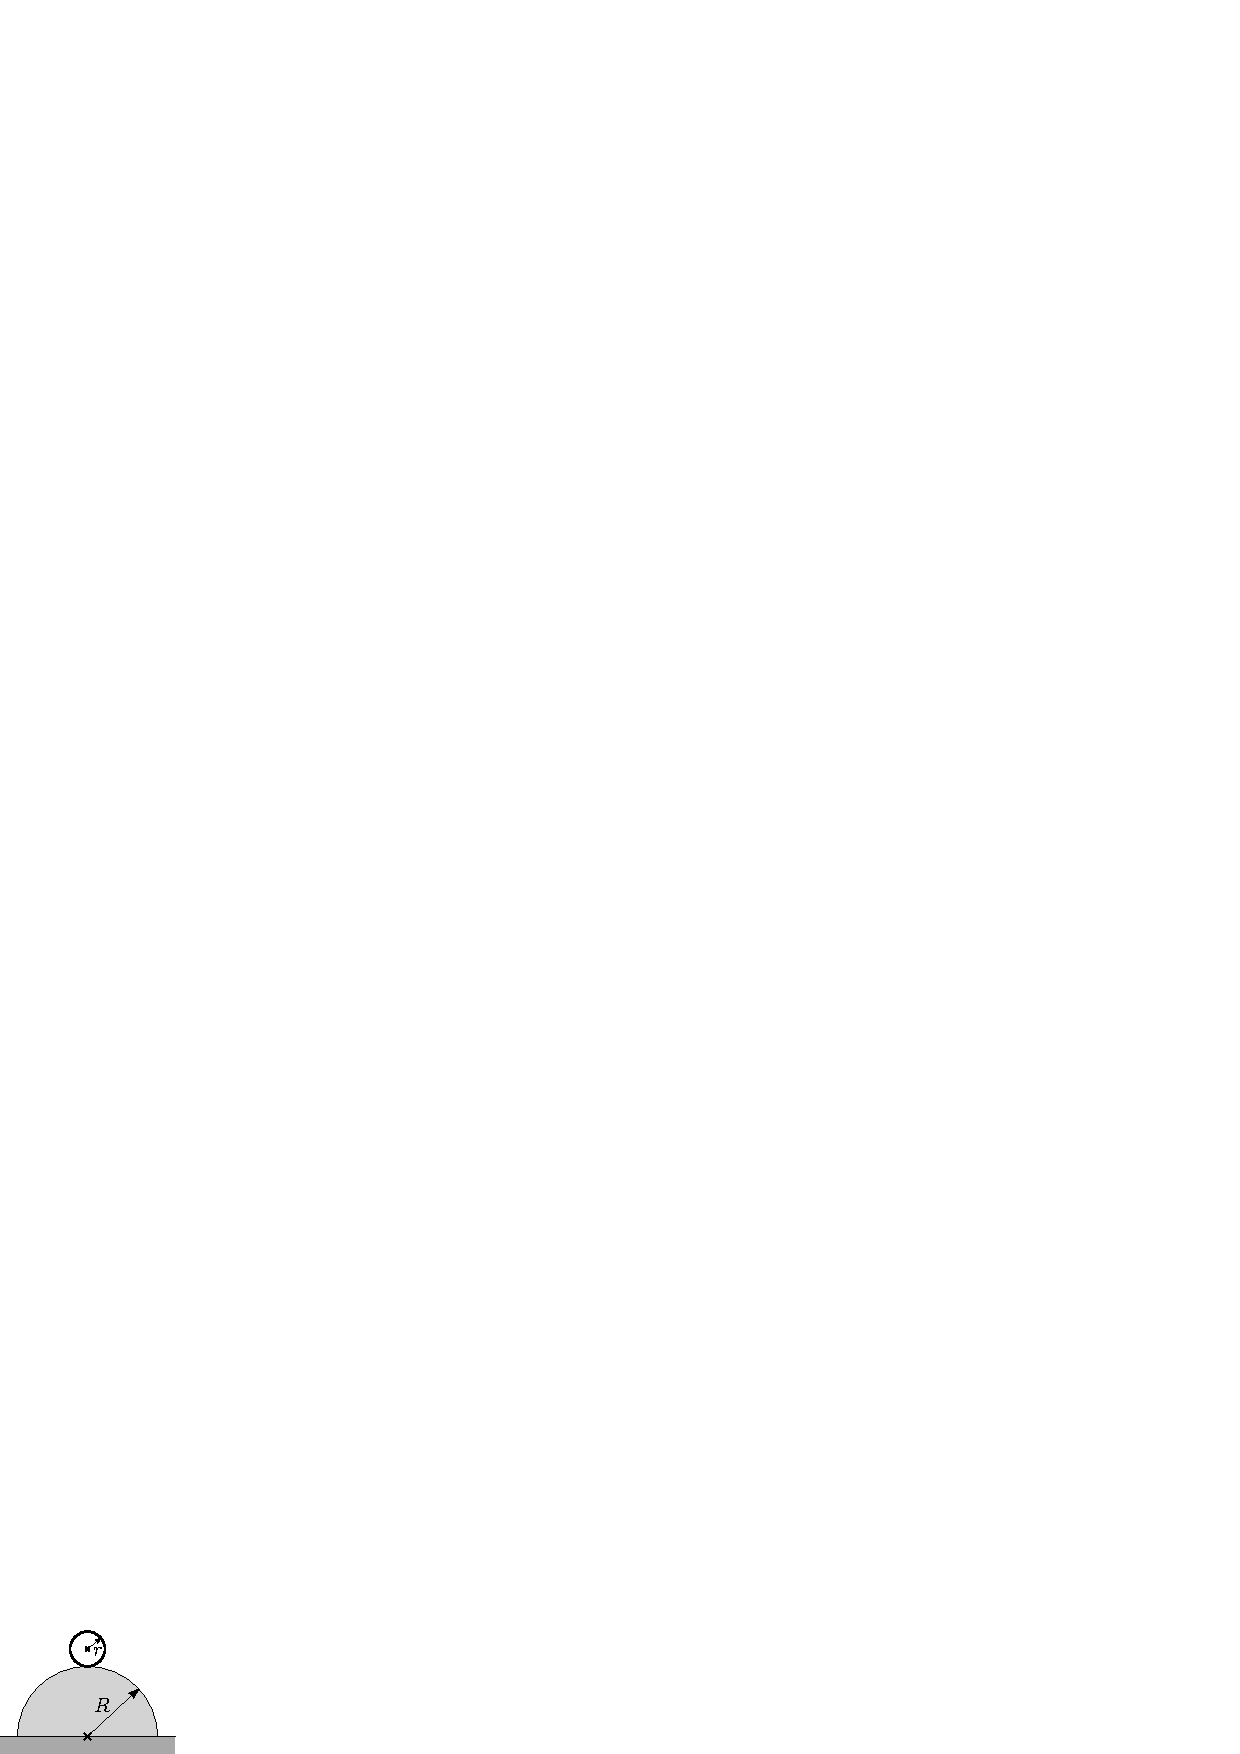
\includegraphics[width=\linewidth]{2010-lahg-03-silindri_joonis_ipe}
\end{wrapfigure}

Alusele kinnitatud poolsilindril raadiusega $R$
lebab selle kõrgeimas punktis seest tühi silinder
raadiusega $r$. Mingisugusel hetkel nihkub keha natuke tasakaalust välja ja
selle tulemusel hakkab libisemiseta veerema (hõõrdetegur on väga suur). Leidke, kui kõrgel aluse kohal keha
poolsilindri pinnast eraldub. \emph{Vihje:} kui veereva silindri mass on $m$ ja
ta masskese liigub kiirusega $v$, on ta kineetiline energia $m v^2$ (ilma
kordajata $\frac12$!).
\fi
}

% Ü26
\ylDisplay{Sfäär} % Ülesande nimi
{Andre Sääsk} % Autor
{lahtine} % Voor
{2005} % Aasta
{G 6} % Ülesande nr.
{5} % Raskustase
{
% Teema: Dünaamika
\ifStatement
Üks osa Pariisi Cité des Sciences teadusmuuseumi kompleksist --- La Géode --- kujutab endast hiigelsuurt sfääri raadiusega $R = \SI{18}{m}$, mille sees asub maailma suurim kinoekraan (vt joonist). Hoonet väljastpoolt imetlev uudishimulik koolipoiss otsustab tabada selle hoone tipp-punkti tennisepalliga. Kui suure minimaalse kiirusega $v$ peaks ta palli viskama, et palli liikumise trajektoor lõikuks hoone välispinnaga vaid ühes punktis --- hoone tipp-punktis --- ja see oleks ühtlasi ka palli liikumise trajektoori kõrgeimaks punktiks? Pall alustab liikumist kõrgusel $h = \SI{1,5}{m}$.

\begin{center}
	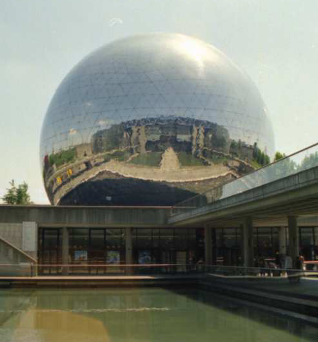
\includegraphics[width=0.5\linewidth]{2005-lahg-06-yl}
\end{center}
\fi
}

% Ü27
\ylDisplay{Anum} % Ülesande nimi
{Tundmatu autor} % Autor
{lahtine} % Voor
{2005} % Aasta
{G 7} % Ülesande nr.
{5} % Raskustase
{
% Teema: Dünaamika
\ifStatement
Siledal pinnal asub kerge ristkülikuline anum, mis on täidetud vedelikuga tihedusega $\rho_0$, vedeliku ruumala on $V_0$. Anuma põhja sattunud põrnikas ruumalaga $V$ ja tihedusega $\rho$ hakkab anuma põhja suhtes roomama kiirusega $u$. Millise kiirusega hakkab anum pinnal liikuma? Anuma mass on tühine, veetase jääb kogu aeg horisontaalseks. Eeldada, et pinna ja anuma vahel hõõre puudub.
\fi
}

% Ü28
\ylDisplay{Mullitaja} % Ülesande nimi
{Jaak Kikas} % Autor
{lõppvoor} % Voor
{2005} % Aasta
{G 7} % Ülesande nr.
{5} % Raskustase
{
% Teema: Dünaamika
\ifStatement
Veekogu põhjas asub mullitaja --- õhuballoon väikese avausega, millest võrdsete ajavahemike $\Delta t = \SI{1}{s}$ järel väljuvad õhumullid raadiusega $R = \SI{0,3}{mm}$. Taolise mullikese liikumisel vees mõjub sellele takistusjõud $F = 6\pi \eta Rv$, kus $\eta$ on vedeliku voolamistakistust iseloomustav tegur (vedeliku viskoossus, vee korral on selle suuruse väärtuseks \SI{1e-3}{N.s/m^2} ) ja $v$ on mullikese kiirus. Võite lugeda, et mullikese liikumine toimub kogu aeg kiirusega, mis on määratud tingimusega, et kõigi talle mõjuvate jõudude resultant on null. Vee tihedus $\rho = \SI{1000}{kg/m^3}$, raskuskiirendus $g = \SI{9,8}{m/s^2}$, õhurõhk $p_0 = \SI{100}{kPa}$. Mitu korda muutub vahemaa naabermullikeste vahel tõusul põhjast pinnale, kui veekogu sügavus on $H = \SI{27}{m}$?
\fi
}

% Ü29
\ylDisplay{Plokk} % Ülesande nimi
{Tundmatu autor} % Autor
{lahtine} % Voor
{2006} % Aasta
{G 5} % Ülesande nr.
{5} % Raskustase
{
% Teema: Dünaamika
\ifStatement
Kui suure kiirendusega $a_k$ ja mis suunas hakkab liikuma kahest kehast koosneva süsteemi masskese, kui kehad on seotud niidiga, mis on tõmmatud üle ploki (vt joonist)? Kehade massid on $m_1$ ja $m_2$ ($m_1$ < $m_2$), niit on kaalutu ja mitteelastne.
\begin{center}
	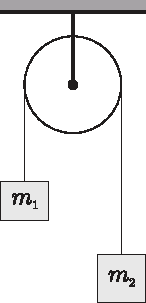
\includegraphics[width=0.25\linewidth]{2006-lahg-05-yl}
\end{center}
\fi
}

% Ü30
\ylDisplay{Kada} % Ülesande nimi
{Oleg Košik} % Autor
{lõppvoor} % Voor
{2006} % Aasta
{G 3} % Ülesande nr.
{5} % Raskustase
{
% Teema: Dünaamika
\ifStatement
Vaatame lihtsa kada ehk ragulka konstruktsiooni. Elastne kummipael tõmmatakse kahe fikseeritud otspunkti vahele, laskmiseks asetatakse kivi paela keskele, pael tõmmatakse koos kiviga pingule ja lastakse vabaks. Kivi lastakse lendu horisontaaltasandi suhtes nurga $\alpha = \SI{10}{\degree}$ all. Leidke, kui kaugele peab laskja tõmbama kivi, et tabada märki, mis asub kadast $L = \SI{25}{m}$ kaugusel ning sellega samal kõrgusel. Kui suurt jõudu peab ta selleks paelale rakendama? Kummipaela pikkus pingestamata olekus on $l = \SI{60}{cm}$, mis on ühtlasi ka paela kinnituspunktide vahekaugus. Pael lugeda kaalutuks ning jäikusteguriga $k = \SI{50}{N/m}$. Kivi mass on $m = \SI{20}{g}$. Õhutakistusega ei ole vaja arvestada. Raskusjõu mõju kivi kiirendamisel kadas pole vaja arvestada.
\fi
}

% Ü31
\ylDisplay{Hooratas} % Ülesande nimi
{Valter Kiisk} % Autor
{lõppvoor} % Voor
{2007} % Aasta
{G 4} % Ülesande nr.
{5} % Raskustase
{
% Teema: Dünaamika
\ifStatement
Hooratas raadiusega $R$ pöörleb nurkkiirusega $\omega$. Lihtsuse huvides võib hooratast vaadelda peenikese rõngana (pöörlemistelg ühtib rõnga teljega).\\
\osa Milline on energia salvestustihedus $w$ (kineetiline energia massiühiku kohta) hoorattas?\\
\osa Hooratas on valmistatud süsinikkiuga armeeritud polümeerist, mille tõmbetugevus $\sigma\idx{max} = \SI{2,4e9}{Pa}$ ja tihedus $\rho = \SI{1500}{kg/m^3}$. Hinnake energia salvestustiheduse maksimaalselt võimalikku väärtust sellises hoorattas (andes numbrilise vastuse).

\emph{Vihje}. Tõmbetugevus on maksimaalne jõud ristlõike pindala kohta, mida antud materjal talub ilma purunemata.
\fi
}

% Ü32
\ylDisplay{Klaaskuul} % Ülesande nimi
{Aigar Vaigu} % Autor
{piirkonnavoor} % Voor
{2008} % Aasta
{G 6} % Ülesande nr.
{5} % Raskustase
{
% Teema: Dünaamika
\ifStatement
Klaaskuul kukkus vertikaalselt alla libedale horisontaalsele põrandale ning purunes kolmeks tükiks, mis lendasid mööda põrandat laiali. Sündmus jäädvustati fotol (vt joonist). Tükkide kujutised osutusid välja venitatuks, sest säriaeg oli võrdlemisi pikk. Millised olid kuuli tükkide masside suhted? Hõõrdejõud tükkide liikumisel lugeda tühiselt väikeseks. Fotoobjektiivi optiline peatelg oli pildistamisel vertikaalne

\begin{center}
	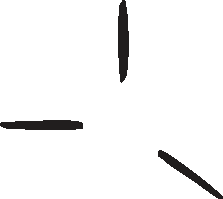
\includegraphics[width=0.6\linewidth]{2008-v2g-06-yl}
\end{center}
\fi
}

% Ü33
\ylDisplay{Maaler} % Ülesande nimi
{Valter Kiisk} % Autor
{lahtine} % Voor
{2010} % Aasta
{G 5} % Ülesande nr.
{5} % Raskustase
{
% Teema: Dünaamika
\ifStatement
Maaler on seina ülemise osa värvimiseks roninud kõrge, peaaegu vertikaalse
redeli tippu. Ettevaatamatu liigutuse tulemusena hakkab redel kukkuma ümber. Kas
vähemohtlik oleks redelist kohe lahti lasta või pigem klammerduda redeli külge?
Põrand on lai ja tühi, nii et (redeli) kukkumist ei takista miski. Redeli alumine
ots ei libise.
\emph{Vihje.} homogeensel vardal pikkusega $l$ ja massiga $m$ on ümber otsa
nurkkiirusega $\omega$ pööreldes kineetiline energia $\frac{m l^2 \omega^2}{6}$.
\fi
}

% Ü34
\ylDisplay{Benji-hüpe} % Ülesande nimi
{Andreas Valdmann} % Autor
{piirkonnavoor} % Voor
{2010} % Aasta
{G 6} % Ülesande nr.
{5} % Raskustase
{
% Teema: Dünaamika
\ifStatement
Benji-hüppaja massiga $m=\SI{80}{kg}$ kasutab köit pikkusega $l=\SI{35}{m}$, mille jäikustegur $k=\SI{60}{N/m}$. Kui kõrgele maapinnast tuleks tõsta hüppeplatvorm, et jääks ohutusvaru $h=\SI{5}{m}$? Mis on suurim kiirus, mille hüppaja saavutab? Raskuskiirendus $g=\SI{9.8}{m/s^2}$. Hüppaja mõõtmetega arvestama ei pea. 
\fi
}

% Ü35
\ylDisplay{Vai} % Ülesande nimi
{Jaak Kikas} % Autor
{piirkonnavoor} % Voor
{2006} % Aasta
{G 10} % Ülesande nr.
{7} % Raskustase
{
% Teema: Dünaamika
\ifStatement
Vertikaalset vaia pikkusega $L$ ja massiga $M$ lüüakse pinnasesse nii, et tema otsa pihta lastakse kõrguselt $H\gg L$ vaia otsast kukkuda koormisel massiga $m$. Lööki vaia pihta võib lugeda absoluutselt mitteelastseks, st pärast raskuse ja vaia kokkupuudet liiguvad nad kui üks tervik. Pinnase takistusjõud on $F = F_0 + kl$, kus $l$ on maa sees oleva vaiaosa pikkus. Kui suur on löökide arv $N$, mis on vajalik selleks, et vai täies pikkuses maasse lüüa? Võite eeldada, et ühekordse löögi tagajärjel nihkub vai sügavamale väikese osa võrra oma pikkusest.
\fi
}

% Ü36
\ylDisplay{Plokid} % Ülesande nimi
{Mihkel Kree} % Autor
{piirkonnavoor} % Voor
{2008} % Aasta
{G 9} % Ülesande nr.
{8} % Raskustase
{
% Teema: Dünaamika
\ifStatement
Polüspast ehk liitplokk koosneb seitsmest plokist (vt. joonist). Koormiste massid $M$ ja $\gamma M$ on näidatud joonisel. Missuguse kiirendusega hakkavad liikuma äärmised koormised? Mis tingimust peab rahuldama suurus $\gamma$, et äärmised koormised hakkaksid langema? Plokkide ja nööri mass jätta arvestamata ning nöör lugeda venimatuks. 

\begin{center}
	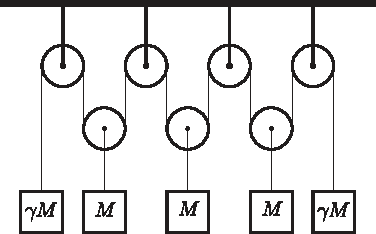
\includegraphics[width=0.6\linewidth]{2008-v2g-09-yl}
\end{center}
\fi
}

% Ü37
\ylDisplay{Rong} % Ülesande nimi
{Tundmatu autor} % Autor
{lahtine} % Voor
{2006} % Aasta
{G 10} % Ülesande nr.
{9} % Raskustase
{
% Teema: Dünaamika
\ifStatement
Rong sõidab kiirusega $v = \SI{100}{km/h}$ ja pidurdab järsult (blokeerides rattad). Graafikul on toodud rongi rataste ja rööbaste vahelise hõõrdeteguri $\mu$ sõltuvus kiirusest (\si{km/h}).\\
\osa Kui pikk on rongi täieliku peatumiseni kulunud aeg?\\
\osa Kui suur on pidurdusmaa pikkus? Mõlemad vastused tuleb leida
graafikualuste pindaladena sobilikult valitud teljestikes.

\begin{center}
	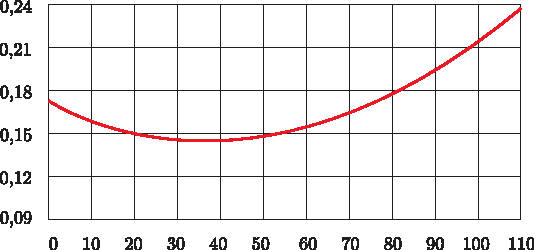
\includegraphics[width=\linewidth]{2006-lahg-10-yl}
\end{center}
\fi
}

% Ü38
\ylDisplay{Värinaalarm} % Ülesande nimi
{Jaan Kalda} % Autor
{lahtine} % Voor
{2011} % Aasta
{G 9} % Ülesande nr.
{9} % Raskustase
{
% Teema: Dünaamika
\ifStatement
Uurime mobiiltelefoni liikumist nõrgalt kaldus pinnal värinaalarmi töötamise
ajal lihtsustatud mudeli abil.
Kujutagu lauale asetatud mobiil risttahukat massiga $M$, mille sees liigub
üles-alla väike keha massiga $m$.
Liikugu see keha ajahetkedel $t=0, 2\tau, 4\tau, \ldots$ vahemaa $x$ võrra
hetkeliselt üles ning ajahetkedel $t=\tau, 3\tau, 5\tau, \ldots$ algasendisse
tagasi.
Olgu mobiiltelefoni ja laua vaheline hõõrdetegur $\mu$ ning laua kaldenurk
$\alpha \ll 1$. Mobiiltelefoni ja laua vahelised põrked lugege absoluutselt
plastseiks.
Millise keskmise kiirusega $u$ hakkab mobiiltelefon mööda lauda liikuma?
\fi
}

% Ü39
\ylDisplay{Kuulid} % Ülesande nimi
{Jaan Kalda} % Autor
{lõppvoor} % Voor
{2006} % Aasta
{G 10} % Ülesande nr.
{10} % Raskustase
{
% Teema: Dünaamika
\ifStatement
\begin{wrapfigure}[8]{r}{0.3\textwidth}
	\begin{center}
		\vspace{-25pt}
		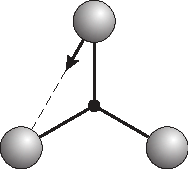
\includegraphics[width=\linewidth]{2006-v3g-10-yl}
	\end{center}
\end{wrapfigure}
Joonisel kujutatud süsteem koosneb kolmest võrdkülgse kolmnurga tippudes paiknevast kuulist massiga $m$ ja kolmest kergest vardast pikkusega $l$, mis on omavahel šarniirselt ühendatud (liigendiga). Süsteem lebab hõõrdevabalt siledal horisontaalpinnal. Ühte kuuli lükatakse teatud lühiajalise jõuga nii, et see omandab kiiruse $v_0$, mis on suunatud naaberkuuli poole. Leidke teiste kuulide kiiruste suunad ja moodulid ning kõigi kuulide kiirendused vahetult peale esimese kuuli lükkamist.
\fi
}
\newpage\subsection{\protect\StrSubstitute{Elektriahelad}{-}{ }}

% Ü40
\ylDisplay{Mõõteriistad} % Ülesande nimi
{Koit Timpmann} % Autor
{lõppvoor} % Voor
{2006} % Aasta
{G 1} % Ülesande nr.
{1} % Raskustase
{
% Teema: Elektriahelad
\ifStatement
Vooluringis on ampermeeter ja voltmeeter ühendatud jadamisi. Klemmidele on rakendatud pinge $U = \SI{9}{V}$. Kui voltmeetriga ühendada rööbiti takisti $R$, väheneb voltmeetri näit kaks korda, ampermeetri näit aga suureneb kaks korda. Kui suurt pinget näitas voltmeeter enne ja pärast takisti ühendamist?

\begin{center}
	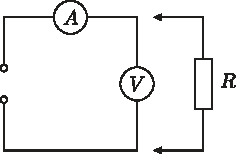
\includegraphics[width=0.5\linewidth]{2006-v3g-01-yl}
\end{center}
\fi
}

% Ü41
\ylDisplay{Elektriküünlad} % Ülesande nimi
{Valter Kiisk} % Autor
{piirkonnavoor} % Voor
{2009} % Aasta
{G 4} % Ülesande nr.
{2} % Raskustase
{
% Teema: Elektriahelad
\ifStatement
Jõulukaunistuse valmistamiseks otsis Juku välja 10
taskulambipirni (nimipinge \SI{3}V, võimsus \SI{0.6}W) ja alaldi klemmipingega \SI{5}V.
Seejärel koostas ta skeemi, mis on kujutatud joonisel.\\
\osa Kui suur peab olema
takisti $R$ takistus, et pinge lampidel ei ületaks nimipinget?\\
\osa Skeemi sisselülitamisel avastas Juku, et lambid põlevad oodatust tuhmimalt. Selgus, et alaldi
klemmipinge oli koormusega langenud \SI{4}V-ni ning pinge lampidel \SI{2,3}V-ni. Kui suur
tuleks valida takisti $R$ väärtus, et lambid põleksid normaalse heledusega?

\begin{center}
	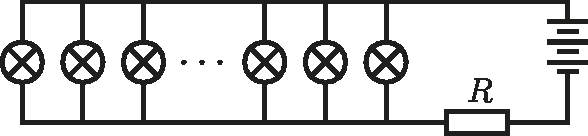
\includegraphics[width=0.8\linewidth]{2009-v2g-04-yl}
\end{center}
\fi
}

% Ü42
\ylDisplay{Päikesepaneel} % Ülesande nimi
{Mihkel Pajusalu} % Autor
{lõppvoor} % Voor
{2010} % Aasta
{G 3} % Ülesande nr.
{2} % Raskustase
{
% Teema: Elektriahelad
\ifStatement
Joonisel on kujutatud päikesepaneeli läbiva voolu sõltuvus klemmipingest.
Määrake paneeli klemmidega ühendatud koormise takistus, mille korral on koormisel eralduv
võimsus maksimaalne.

\begin{center}
	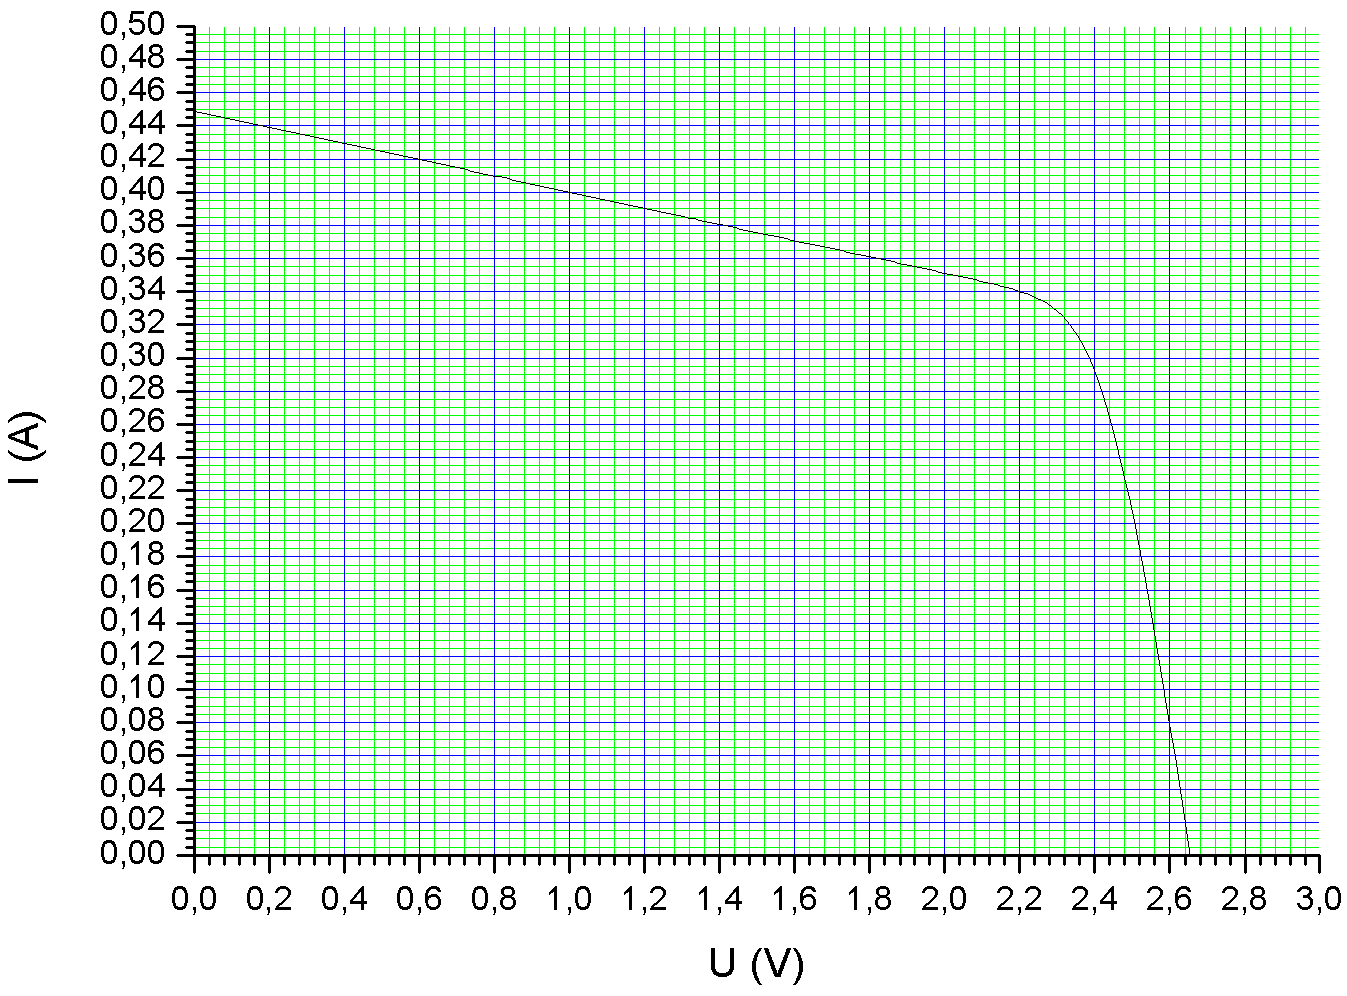
\includegraphics[width=0.9\linewidth]{2010-v3g-03-paneel_yl.png}
\end{center}
\fi
}

% Ü43
\ylDisplay{Ampermeetrid} % Ülesande nimi
{Tundmatu autor} % Autor
{lahtine} % Voor
{2008} % Aasta
{G 4} % Ülesande nr.
{3} % Raskustase
{
% Teema: Elektriahelad
\ifStatement
Vooluahelasse on ühendatud neli ühesugust ampermeetrit, igaüks sisetakistusega $r$, ja takisti $R$. Esimese kahe ampermeetri näidud on $I_1= \SI{3}{A}$ ja $I_2= \SI{5}{A}$. Leida takistuste suhte $R/r$ arvuline väärtus.

\begin{center}
	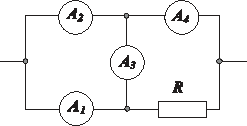
\includegraphics[width=0.6\linewidth]{2008-lahg-04-yl}
\end{center}
\fi
}

% Ü44
\ylDisplay{Patarei} % Ülesande nimi
{Taavi Pungas} % Autor
{piirkonnavoor} % Voor
{2011} % Aasta
{G 6} % Ülesande nr.
{3} % Raskustase
{
% Teema: Elektriahelad
\ifStatement
Patarei ühendatakse jadamisi takistiga takistusega $R$ ja ampermeetriga, mis näitab voolutugevuseks $I_1$. Kui lisada jadamisi veel üks takisti takistusega $R$, näitab ampermeeter voolutugevuseks $I_2$. Leidke, mis vahemikku jääks suhe $I_2/I_1$, kui vooluallika sisetakistus $r$ oleks\\
\osa väiksem kui $R$,\\
\osa suurem kui $R$.
\fi
}

% Ü45
\ylDisplay{Takistid} % Ülesande nimi
{Aigar Vaigu} % Autor
{lõppvoor} % Voor
{2005} % Aasta
{G 4} % Ülesande nr.
{4} % Raskustase
{
% Teema: Elektriahelad
\ifStatement
Mitu korda muutub joonisel kujutatud ahelas takistil $A$ eralduv võimsus, kui vahetada alalispingeallika polaarsus? Kõik takistid on võrdse takistusega.

\begin{center}
	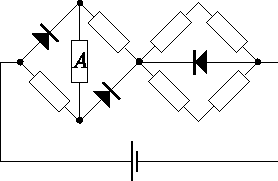
\includegraphics[width=0.6\linewidth]{2005-v3g-04-yl}
\end{center}
\fi
}

% Ü46
\ylDisplay{Elektriskeem} % Ülesande nimi
{Tundmatu autor} % Autor
{lahtine} % Voor
{2006} % Aasta
{G 2} % Ülesande nr.
{4} % Raskustase
{
% Teema: Elektriahelad
\ifStatement
Leida laengud $q_1$, $q_2$ ja $q_3$ kõikidel skeemil toodud kondensaatoritel.

\begin{center}
	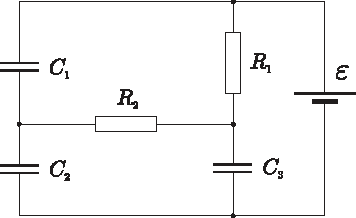
\includegraphics[width=0.7\linewidth]{2006-lahg-02-yl}
\end{center}
\fi
}

% Ü47
\ylDisplay{Skeem} % Ülesande nimi
{Tundmatu autor} % Autor
{lahtine} % Voor
{2009} % Aasta
{G 3} % Ülesande nr.
{4} % Raskustase
{
% Teema: Elektriahelad
\ifStatement
Elemendi $X$ takistus muutub sõltuvalt selle pingest. Kui $U_X \leq \SI{1}{V}$,
siis selle takistus on $R_1 = \SI{1}{\ohm}$, kui aga $U_X > \SI{1}{V}$, siis on takistus $R_2 =
\SI{2}{\ohm}$. Kolm elementi $X$ ühendatakse ideaalse ampermeetriga, nagu näidatud joonisel.
Väljundklemmidele rakendatakse pinge, mille ajaline sõltuvus on toodud graafikul.
Joonestage ampermeetri näidu ajalise sõltuvuse graafik.

\begin{center}
	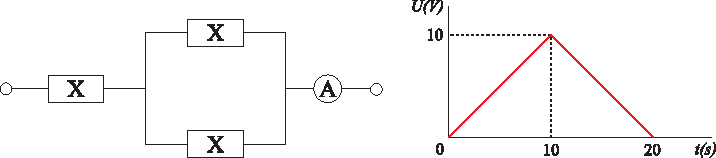
\includegraphics[width=\linewidth]{2009-lahg-03-yl}
\end{center}
\fi
}

% Ü48
\ylDisplay{Takisti} % Ülesande nimi
{Jaan Kalda} % Autor
{piirkonnavoor} % Voor
{2007} % Aasta
{G 7} % Ülesande nr.
{5} % Raskustase
{
% Teema: Elektriahelad
\ifStatement
Oletagem, et me tahame teha takisti takistusega $R = 1 \ohm$, mille takistuse temperatuurisõltuvus oleks toatemperatuuri ümbruses võimalikult väike. Olgu meil kasutada raudtraat ristlõikepindalaga $s = \SI{0,030}{mm^2}$ ja grafiitpulk ristlõikepindalaga $S = \SI{3,0}{mm^2}$. Kuidas valmistada soovitud takistit ja kui pikki grafiitpulga ning terastraadi juppe tuleb seejuures kasutada? Grafiidi ja raua eritakistused on vastavalt $\rho_g = \SI{3,0e5}{\ohm.m}$ ning $\rho_r = \SI{9,7e-8}{\ohm.m}$; takistuse temperatuurikoefitsiendid (suhtelised muutused $\Delta R/R$ temperatuuri kasvamisel ühe kraadi võrra) on $\alpha_g = \SI{-5,0e-3}{K^{-1}}$ ning $\alpha_r = \SI{6,41e-3}{K^{-1}}$
\fi
}

% Ü49
\ylDisplay{Kondensaatoriredel} % Ülesande nimi
{Siim Ainsaar} % Autor
{piirkonnavoor} % Voor
{2007} % Aasta
{G 8} % Ülesande nr.
{5} % Raskustase
{
% Teema: Elektriahelad
\ifStatement
Ühesugustest kondensaatoritest mahtuvusega $C$ on koostatud joonisel näidatud lõpmatu ahel. Leidke ahela kogumahtuvus $C_k$.

\begin{center}
	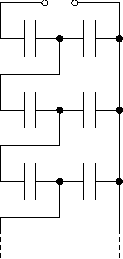
\includegraphics[width=0.3\linewidth]{2007-v2g-08-yl}
\end{center}
\fi
}

% Ü50
\ylDisplay{Traat} % Ülesande nimi
{Jaan Kalda} % Autor
{lõppvoor} % Voor
{2008} % Aasta
{G 7} % Ülesande nr.
{5} % Raskustase
{
% Teema: Elektriahelad
\ifStatement
Ühtlase ristlõikega traati (ristlõike pindala $S = \SI{1}{mm^2}$) venitati nii, et tema erinevad lõigud venisid erinevalt. Enne venitamist oli traadile märgitud jooned iga millimeetri tagant. Joonisel on toodud nende joonte vahekaugused $\Delta$ pärast venitamist sõltuvuses kaugusest traadi ühest otsast $l$ ($l$ on mõõdetud pärast venitamist). Leidke selle nüüdseks 4 meetri pikkuse traadi takistus, arvestades, et traadi materjali tihedus ja eritakistus $\rho = \SI{1e-6}{\ohm.m}$ venitamise tagajärjel ei muutunud.

\begin{center}
	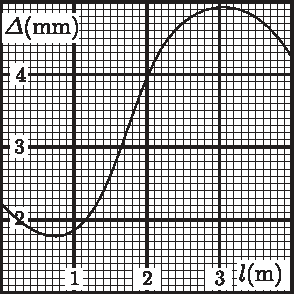
\includegraphics[width=0.6\linewidth]{2008-v3g-07-yl}
\end{center}
\fi
}

% Ü51
\ylDisplay{Kondensaator} % Ülesande nimi
{Aigar Vaigu} % Autor
{piirkonnavoor} % Voor
{2010} % Aasta
{G 7} % Ülesande nr.
{5} % Raskustase
{
% Teema: Elektriahelad
\ifStatement
Muudetava mahtuvusega kondensaator on ühendatud patareiga,
mille klemmide pinge on $U$. Kondensaatori mahtuvust muudetakse laadimisel nii, et
kondensaatori laadimise vool $I$ on konstantne. Leidke patarei võimsus ja kondensaatori laadimisel energia salvestamise kiirus.
Põhjendage võimalikku erinevust.
\fi
}
\newpage


% Ü52
\ylDisplay{Kondensaatorid} % Ülesande nimi
{Mihkel Rähn} % Autor
{piirkonnavoor} % Voor
{2006} % Aasta
{G 7} % Ülesande nr.
{6} % Raskustase
{
% Teema: Elektriahelad
\ifStatement
\begin{wrapfigure}{r}{0.45\textwidth}
	\begin{center}
		\vspace{-25pt}
		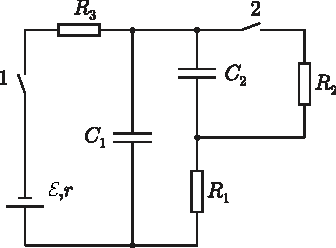
\includegraphics[width=\linewidth]{2006-v2g-07-yl}
	\end{center}
\end{wrapfigure}
Joonisel toodud elektriskeemil on vooluallikas elektromotoorjõuga $\mathcal E$ ja sisetakistusega $r$, kolm takistit takistustega $R_1 = R_2 = R_3 = R$ ning kondensaatorid mahtuvustega $C_1$ ja $C_2$. Arvutage, kui suured on elektrilaengud kondensaatoritel pärast pika aja möödumist, kui:\\
\osa lüliti 1 on suletud, lüliti 2 on avatud;\\
\osa mõlemad lülitid on suletud;\\
\osa eelmisest seisust avatakse mõlemad lülitid üheaegselt. 
\fi
}

% Ü53
\ylDisplay{Kondensaatorid} % Ülesande nimi
{Mihkel Kree} % Autor
{lõppvoor} % Voor
{2009} % Aasta
{G 3} % Ülesande nr.
{6} % Raskustase
{
% Teema: Elektriahelad
\ifStatement
Koosnegu kondensaatorite süsteem viiest kondensaatorist. Alghetkel on kolm neist laenguta ning kahel paikneb laeng $q$ (vt joonist). Missugune laeng koguneb keskmisele kondensaatorile, kui süsteem on jõudnud tasakaaluolekusse?

\begin{center}
	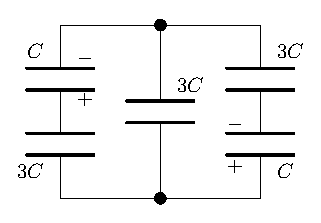
\includegraphics[width=0.42\linewidth]{2009-v3g-03-G_kondensaatorid.eps}
\end{center}
\fi
}

% Ü54
\ylDisplay{Aku laadimine} % Ülesande nimi
{Valter Kiisk} % Autor
{piirkonnavoor} % Voor
{2008} % Aasta
{G 8} % Ülesande nr.
{7} % Raskustase
{
% Teema: Elektriahelad
\ifStatement
Teatava akumulaatori elektromotoorjõud kasvab laadimise käigus nõnda, nagu kujutatud joonisel. Samas on toodud ka elektriskeem, mida Juku kavatseb kasutada sellise akumulaatori laadimiseks. Pingeallika klemmidel on pinge \SI{6}{V}. Nii pingeallika kui ka aku sisetakistuse võib lugeda tühiseks. Kuidas peaks Juku valima takistite $R_1$ ja $R_2$ väärtused, kui ta taotleb, et maksimaalne laadimisvool ei ületaks \SI{100}{mA} ja laadimisvool muutuks nulliks, kui akumulaator on täielikult laetud? 

\begin{center}
	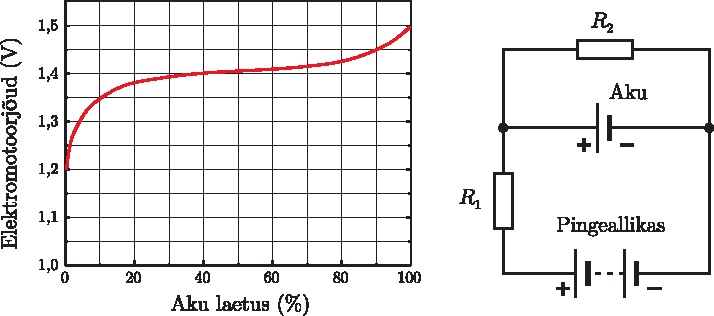
\includegraphics[width=\linewidth]{2008-v2g-08-yl}
\end{center}
\fi
}

% Ü55
\ylDisplay{Närvirakk} % Ülesande nimi
{Andres Laan} % Autor
{lõppvoor} % Voor
{2011} % Aasta
{G 9} % Ülesande nr.
{7} % Raskustase
{
% Teema: Elektriahelad
\ifStatement
Närviraku membraani võib vaadelda kui õhukest kilet mahtuvusega $C$, mida läbivad ioonkanalid, mis võimaldavad laengutel liikuda läbi
membraani. Närviraku elektrilise tasakaalu seisukohast on olulisteks ioonideks
naatrium ja kaalium. Kui naatriumioon (laenguga $+e$) läbib ioonkanali (sisenedes närvirakku), siis sooritavad keemilised jõud töö $e\mathcal{E}_{\mathrm{Na}}$, st võib öelda, et
naatriumioonidele mõjub ioonkanalis elektromotoorjõud $\mathcal{E}_{\mathrm{Na}}$. Kaaliumioonide
puhul on kanali läbimise protsess täpselt samasugune, kuid efektiivne elektromotoorjõud on sel puhul $\mathcal{E}_{\mathrm{K}}$ ($\neq \mathcal{E}_{\mathrm{Na}}$). Peale keemiliste jõudude töö toimivad
laengu liikumisel ioonkanalis ka hõõrdejõud, mida saab kirjeldada elektrilise
takistuse abil: naatriumioonide jaoks on membraani elektriline takistus $R_{\mathrm{Na}}$ ja kaaliumioonide jaoks $R_{\mathrm{K}}$. Millise laengu omandab närviraku membraan
elektrilise tasakaalu saabudes? 
\fi
}

% Ü56
\ylDisplay{Jõulukaunistus} % Ülesande nimi
{Valter Kiisk} % Autor
{lõppvoor} % Voor
{2010} % Aasta
{G 8} % Ülesande nr.
{8} % Raskustase
{
% Teema: Elektriahelad
\ifStatement
Jõulukaunistuse hankimiseks majandussurutise tingimustes otsustas Juku
ühendada jadamisi kokku 50 valgusdioodi ja toita seda ahelat läbi alaldusdioodi $D$ otse
võrgupingega (vt joonist). Voolu piiramiseks on ahelasse lülitatud takisti
ning voolu pulsatsiooni väljasilumiseks kondensaator. Pinge alaldusdioodil on
tühine, igal valgusdioodil aga $U_d=\SI{3}{V}$. Kui suure takistusega $R$ ja maksimumvõimsusega $N$ tuleks valida
takisti, kui valgusdioodid taluvad voolu kuni $I=\SI{20}{mA}$? Kui suure mahtuvusega $C$
kondensaator kindlustab, et voolutugevuse pulsatsioon jääb $\alpha=\num{5}\%$ piiresse? Võrgupinge
sagedus on $f=\SI{50}{Hz}$ ning amplituudväärtus $U_0=\SI{311}{V}$.

\begin{center}
	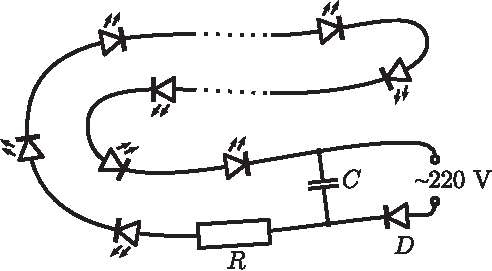
\includegraphics[scale=0.75]{2010-v3g-08-elektrikuunlad2}
\end{center}
\fi
}
\newpage\subsection{\protect\StrSubstitute{Elektrostaatika}{-}{ }}

% Ü57
\ylDisplay{Juhe} % Ülesande nimi
{Tundmatu autor} % Autor
{lahtine} % Voor
{2005} % Aasta
{G 5} % Ülesande nr.
{3} % Raskustase
{
% Teema: Elektrostaatika
\ifStatement
Sirgjooneline juhe asub sügaval maa all ühtlases pinnases. Lekkevool ühikulise pikkusega juhtmest on $i$. Leidke lekkevoolu tihedus (\si{A/m^2}) kaugusel $r$ juhtmest. Juhtme pikkus on palju suurem kui $r$. Lekkevool on konstantne piki juhet.

\emph{Märkus}. lekkevooluks nimetatakse voolu, mis levib isolaatorites. 
\fi
}

% Ü58
\ylDisplay{Kuulikesed} % Ülesande nimi
{Tundmatu autor} % Autor
{lahtine} % Voor
{2005} % Aasta
{G 4} % Ülesande nr.
{4} % Raskustase
{
% Teema: Elektrostaatika
\ifStatement
Seitse ühesugust laetud kuulikest laenguga $q$ on seotud omavahel samast materjalist võrdse algpikkusega elastsete niitidega ja saavad liikuda vaid ühes fikseeritud tasapinnas (vt joonist). Vahemaa kahe suvalise naaberkuulikese vahel tasakaalu olekus on $l$. Leidke tõmbepinged niitides.

\begin{center}
	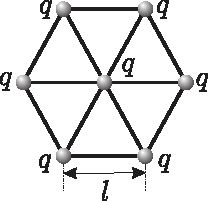
\includegraphics[width=0.35\linewidth]{2005-lahg-04-yl}
\end{center}
\fi
}

% Ü59
\ylDisplay{Vooluring} % Ülesande nimi
{Valter Kiisk} % Autor
{piirkonnavoor} % Voor
{2005} % Aasta
{G 4} % Ülesande nr.
{4} % Raskustase
{
% Teema: Elektrostaatika
\ifStatement
Takisti takistuse määramiseks koostati kaks erinevat vooluringi kasutades voltmeetrit, ampermeetrit ja vooluallikat (vt joonist). Leidke avaldis takistuse $R$ arvutamiseks, kui vasakpoolse skeemi järgi mõõtes saadi voltmeetri näiduks $U_1$ ja ampermeetri näiduks $I_1$ ning parempoolse skeemi järgi mõõtes aga vastavalt $U_2$ ja $I_2$. Vooluallika elektromotoorjõud on muutumatu ning sisetakistus tühine. Mõõteriistade sisetakistused ei ole teada.

\begin{figure}[h]
	\centering
	\subfloat{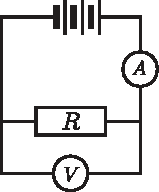
\includegraphics[width=0.4\textwidth]{2005-v2g-04-yl1}}
	\hfill
	\subfloat{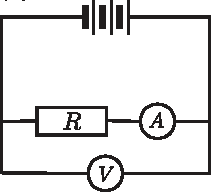
\includegraphics[width=0.45\textwidth]{2005-v2g-04-yl2}}
\end{figure}

\fi
}

% Ü60
\ylDisplay{Tolmukübe} % Ülesande nimi
{Aigar Vaigu} % Autor
{piirkonnavoor} % Voor
{2006} % Aasta
{G 8} % Ülesande nr.
{4} % Raskustase
{
% Teema: Elektrostaatika
\ifStatement
Tolmukübe massiga $m = \SI{1e-9}{g}$ on kondensaatori horisontaalsete plaatide vahel tasakaalus. Laengu pindtihedus kondensaatori plaatidel $\sigma = \SI{2,6e-5}{C/m^2}$. Kui suur on tolmukübeme elektrilaeng? Millise kiirendusega hakkaks tolmukübe langema, kui kondensaatori polaarsus muuta vastupidiseks? Eeldada, et elektriväli kondensaatori plaatide vahel on homogeenne. Õhutakistust mitte arvestada. Elektriline konstant $\varepsilon_0 = \SI{8,85e-12}{F/m}$, õhu dielektriline läbitavus $\varepsilon \approx 1$.
\fi
}

% Ü61
\ylDisplay{Kuulikesed} % Ülesande nimi
{Tundmatu autor} % Autor
{lahtine} % Voor
{2007} % Aasta
{G 7} % Ülesande nr.
{4} % Raskustase
{
% Teema: Elektrostaatika
\ifStatement
Kaks ühesugust kuulikest, millest kumbki kannab laengut $q$, asuvad vertikaalsihis kaugusel $H$ üksteisest. Alumine kuulike on jäigalt kinnitatud, ülemine aga hakkab liikuma vertikaalselt alla suunatud algkiirusega $v$. Kui suur on minimaalne kaugus $h$ alumise kuulikeseni, millele suudab läheneda ülemine kuulike? Ülemise kuulikese mass on $m$. Raskuskiirendus on $g$.
\fi
}

% Ü62
\ylDisplay{Laetud rõngas} % Ülesande nimi
{Tundmatu autor} % Autor
{lahtine} % Voor
{2009} % Aasta
{G 4} % Ülesande nr.
{4} % Raskustase
{
% Teema: Elektrostaatika
\ifStatement
Peenikesest traadist rõngas raadiusega $R$ on ühtlaselt laetud negatiivse laenguga $Q$. Elektron massiga $m$ ja laenguga $e$ läheneb rõngale mööda sirget, mis on risti rõnga tasandiga ning läbib rõnga keskpunkti. Millist tingimust peab rahuldama elektroni kiirus punktis, mis asub kaugusel $d = R\sqrt 3$ rõnga keskpunktist, et elektron saaks rõngast läbi lennata?
\fi
}

% Ü63
\ylDisplay{Liikuv laeng} % Ülesande nimi
{Jaan Kalda} % Autor
{piirkonnavoor} % Voor
{2009} % Aasta
{G 6} % Ülesande nr.
{4} % Raskustase
{
% Teema: Elektrostaatika
\ifStatement
Laetud osake laengu ja massi suhtega $q/m = \SI{1}{C/kg}$ seisab algselt paigal. Seejärel hakkab ta liikuma $x$- ja $y$-telje sihis
toimivate elektrivälja impulsside mõjul. Elektrivälja vastavate komponentide $E_x$ ja $E_y$ sõltuvus ajast on toodud graafikul (graafiku mastaap
ei ole korrektne, juhenduda tuleb graafikul näidatud numbritest impulsi
kestvuse $\tau = \SI{1}{ms}$ ja amplituudi $E_0 = \SI{1}{kV/m}$ ning perioodi $T = \SI{2}{s}$
jaoks). Visandage osakese trajektoor ja leidke keskmine kiirus (visandi tegemisel ja arvutustes võib lugeda ajavahemiku $\tau = \SI{1}{ms}$ jooksul
toimuvad muutused hetkelisteks). 

\begin{center}
	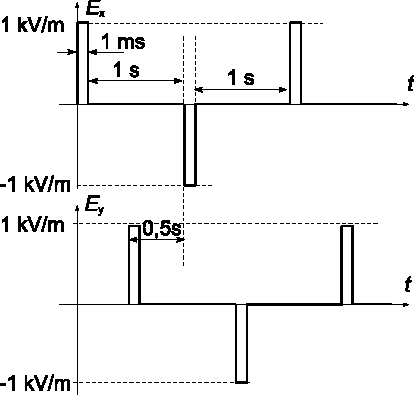
\includegraphics[width=0.6\linewidth]{2009-v2g-06-yl}
\end{center}
\fi
}

% Ü64
\ylDisplay{Ioonmootor} % Ülesande nimi
{Mihkel Pajusalu} % Autor
{lahtine} % Voor
{2010} % Aasta
{G 6} % Ülesande nr.
{4} % Raskustase
{
% Teema: Elektrostaatika
\ifStatement
Kosmosesond on varustatud lihtsa ioonmootoriga, mis koosneb ksenooni
ioonide $\mathrm{Xe}^+$ allikast ja kahest elektroodist, mille vahele rakendatakse pinge
$U$ ja mille vahelist maad läbides ioone kiirendatakse. Kui suurt kogust
(mass) ksenooni on vaja, et selle mootoriga sondi kiirust tõsta
$\Delta v=\SI{1}{km/s}$ võrra?
%
Ksenooni aatommass $\mu=\SI{131,29}{g/mol}$, kosmosesondi mass $M=\SI{1000}{kg}$, kiirendav pinge
$U=\SI{100}{kV}$, elementaarlaeng $e=\SI{1,60 e-19}{C}$, Avogadro arv
$N_A= \SI{6,02 e23}{mol^{-1}}$.
\fi
}

% Ü65
\ylDisplay{Lendav elektronkahur} % Ülesande nimi
{Siim Ainsaar} % Autor
{lõppvoor} % Voor
{2006} % Aasta
{G 6} % Ülesande nr.
{5} % Raskustase
{
% Teema: Elektrostaatika
\ifStatement
Jaan Tatikal tuli järjekordne lennumasinaidee, mida ta kohe realiseerima tõttas. Ta nimelt ehitas palkidest platvormi, mille alla kinnitas telerist välja lõhutud elektronkahuri koos vajaliku elektroonika ja akuga. Elektrone kiirendav pinge on $U$, voolutugevus elektronkiires $I$. Leidke, kui suurt tõstejõudu $F$ suudab see seade tekitada. Missugust tingimust peaksid $U$ ja $I$ rahuldama, et taoline lennumasin suudaks leiduri õhku tõsta? Kas see on ka realistlik (televiisorites $U \approx \SI{30}{kV}$, $I \approx \SI{100}{\micro A}$)? Relativistlikke efekte pole vaja arvestada; elektroni algkiirus katoodi juures on 0. Eeldage, et kiir üldse moodustub (õhu olemasoluga ärge arvestage). Tatika mass koos platvormi ja seadmega on $m_T \approx \SI{150}{kg}$, raskuskiirendus $g \approx \SI{9,8}{m/s^2}$. Elektroni laengu ja massi suhe $k = e/m_e \approx \SI{1,76e11}{C/kg}$.
\fi
}

% Ü66
\ylDisplay{Elektronkiir} % Ülesande nimi
{Tundmatu autor} % Autor
{lahtine} % Voor
{2008} % Aasta
{G 7} % Ülesande nr.
{5} % Raskustase
{
% Teema: Elektrostaatika
\ifStatement
Kitsas elektronkiir läbib vaakumis tasaparalleelsete plaatide vahelise pilu ja langeb seejärel fluorestseeruvale ekraanile, mis asub plaatide ekraanipoolsemast servast kaugusel $l = \SI{15}{cm}$. Kui plaatidele antakse pinge $U = \SI{50}{V}$, nihkub helendav punkt ekraanil endisest asukohast kaugusele $s = \SI{21}{mm}$. Plaatidevaheline kaugus $d = \SI{18}{mm}$, plaatide mõõtmed elektronide liikumise suunas on $b = \SI{6}{cm}$. Milline on elektronide algkiirus plaatide vahele sattumisel? Elektroni laengu ja massi suhe $e/m \approx \SI{1,76e11}{C/kg}$.
\fi
}

% Ü67
\ylDisplay{Kuup} % Ülesande nimi
{Jaan Kalda} % Autor
{piirkonnavoor} % Voor
{2008} % Aasta
{G 7} % Ülesande nr.
{5} % Raskustase
{
% Teema: Elektrostaatika
\ifStatement
Õhukesest elektrit mittejuhtivast materjalist on valmistatud kuup küljepikkusega $a$. Kuubil on elektrilaeng ühtlase pindtihedusega $\sigma$ (pindtihedus on laeng pinnaühiku kohta). Ühe tahu keskkohta lõigatakse väike ruudukujuline auk mõõtmetega $b \times b$ ($b \ll a$). Leida elektrivälja tugevus kuubi keskpunktis.
\fi
}

% Ü68
\ylDisplay{Sfäärid} % Ülesande nimi
{Kristian Kuppart} % Autor
{lahtine} % Voor
{2011} % Aasta
{G 8} % Ülesande nr.
{6} % Raskustase
{
% Teema: Elektrostaatika
\ifStatement
Kaks juhtivast materjalist sfääri raadiustega $R_1$ ja $R_2$ on ühendatud pika 
juhtmega. Ühele sfääridest antakse mingi laeng. Leidke suhe $\frac{E_1}{E_2}$, kus
$E_1$ ja $E_2$ on elektrivälja tugevused vastavate sfääride pinnal. Eeldage, et
juhtme mahtuvus on tühine ning juhtme pikkus on oluliselt suurem sfääride
raadiustest.
\fi
}

% Ü69
\ylDisplay{Kondensaatorid} % Ülesande nimi
{Oleg Košik} % Autor
{lõppvoor} % Voor
{2005} % Aasta
{G 8} % Ülesande nr.
{7} % Raskustase
{
% Teema: Elektrostaatika
\ifStatement
Kondensaatorid mahtuvustega $2C$ ja $3C$ on ühendatud pingeallikaga, mille pinge on $U$. Osake massiga m ning laenguga $q$ lendab algkiirusega $v$, mis on suunatud paralleelselt kondensaatorite plaatidega (vt joonist). Osake lendab mõlema kondensaatori plaatide vahelt läbi. Mõlema kondensaatori plaatide pikkus on $l$ ning plaatide vahelised kaugused on vastavalt $2d$ ja $d$. Leidke nurk, mille võrra kaldub osake võrreldes esialgse trajektooriga, kui ta väljub joonisel ülemisest kondensaatorist. Eeldada, et see nurk on väike.

\begin{center}
	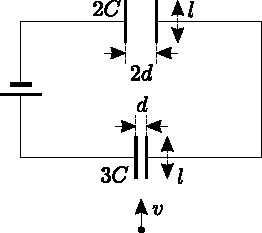
\includegraphics[width=0.6\linewidth]{2005-v3g-08-yl}
\end{center}
\fi
}

% Ü70
\ylDisplay{Kärbes} % Ülesande nimi
{Stanislav Zavjalov} % Autor
{lahtine} % Voor
{2010} % Aasta
{G 7} % Ülesande nr.
{7} % Raskustase
{
% Teema: Elektrostaatika
\ifStatement
Kärbes on otsustanud
lennates püsida ainult ekvipotentsiaalsete pindade peal. Ta lendab sisse ruumi,
mis on täidetud homogeense elektriväljaga $\vec{E}$, välja jõujoontega risti.
Elektriväljas hoitakse paigal ka laengut $-Q$ nii, et kärbse
trajektoori esialgse puutuja ja laengu vahemaa on $d$ (vt. joonist; $-Q < 0$).
Kui lähedale kärbes laengule jõuab? Eeldage, et $Q \le \pi\epsilon_0Ed^2$.
\begin{center}
	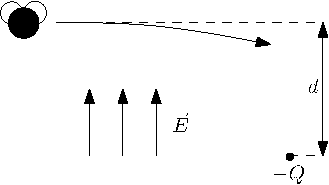
\includegraphics[width=0.4\textwidth]{2010-lahg-07-muha_tekst}
\end{center}
\fi
}

% Ü71
\ylDisplay{Laetud klotsid} % Ülesande nimi
{Tundmatu autor} % Autor
{lahtine} % Voor
{2006} % Aasta
{G 9} % Ülesande nr.
{8} % Raskustase
{
% Teema: Elektrostaatika
\ifStatement
Horisontaalsel siledal dielektrilisel pinnal asuvad kaks laetud klotsi massidega $m$ ja samanimeliste laengutega $q$. Alghetkel on vahemaa nende vahel $l$. Mis tingimusel hakkavad klotsid liikuma ja kui suur on vahemaa $L$ nende vahel, kui liikumine lõppeb? Hõõrdetegur klotside ja pinna vahel on $\mu$. Klotside mõõtmeid ja liikuvate laengute elektromagnetkiirgust mitte arvestada. Pinna dielektriline läbitavus on 1.
\fi
}

% Ü72
\ylDisplay{Kosmoseprügi} % Ülesande nimi
{Siim Ainsaar} % Autor
{lõppvoor} % Voor
{2009} % Aasta
{G 9} % Ülesande nr.
{8} % Raskustase
{
% Teema: Elektrostaatika
\ifStatement
Kaks ühesugust elektriliselt laetud
kuuli, mis on ühendatud ideaalse nööriga, hõljuvad vabalt kosmoses. Kummagi
kera laeng on $q$ ja mass $M$, nööri pikkus on $l$.
Ootamatult lendab nööriga risti selle keskkoha pihta kosmoseprügi tükk massiga $m$ ja kiirusega
$v$ ning jääb nööri külge kinni. Millisele vähimale kaugusele $d$ lähenevad teineteisele kuulid?
Eeldada, et kuulikeste diameetrid on väiksemad kui otsitav kaugus $d$.
\fi
}
\newpage\subsection{\protect\StrSubstitute{Gaasid}{-}{ }}

% Ü73
\ylDisplay{Jalgpall} % Ülesande nimi
{Tundmatu autor} % Autor
{lahtine} % Voor
{2006} % Aasta
{G 1} % Ülesande nr.
{1} % Raskustase
{
% Teema: Gaasid
\ifStatement
Kui suure rõhuni $p_N$ võib pumbata jalgpalli palli kolbpumbaga $N = 40$ pumpamise käigus? Iga pumpamiskäigu jooksul võtab pump atmosfäärist õhu koguse ruumalaga $v = \SI{150}{cm^3}$. Atmosfääri rõhk $p_0 = \SI{0,1}{MPa}$, palli ruumala $V = \SI{3}{l}$. Lugeda, et õhu temperatuur pallis võrdub välistemperatuuriga.
\fi
}

% Ü74
\ylDisplay{Allveelaev} % Ülesande nimi
{Tundmatu autor} % Autor
{lahtine} % Voor
{2007} % Aasta
{G 3} % Ülesande nr.
{1} % Raskustase
{
% Teema: Gaasid
\ifStatement
Uppunud allveelaevadest on inimesed mõnikord pääsenud avades esialgu alumised ventiilid (mida mööda vesi sisse tungib), seejärel ülemise luugi ning siis ise koos õhumulliga veepinnale tõustes. Kui suur osa $k$ laeva ruumalast polnud täidetud veega peale ventiilide avamist, kui laev asus sugavusel $h = \SI{42}{m}$? Merevee tihedus $\rho = \SI{1,03e3}{kg/m^3}$. Õhu rõhk laevas alghetkel $p_0 = \SI{0,1}{MPa}$. Võite lugeda, et vee sisse laskmise käigus õhu temperatuur laevas ei muutu (tänu soojusvahetusele ümbritseva veega).
\fi
}

% Ü75
\ylDisplay{Tuukrid} % Ülesande nimi
{Ott Krikmann} % Autor
{piirkonnavoor} % Voor
{2007} % Aasta
{G 4} % Ülesande nr.
{2} % Raskustase
{
% Teema: Gaasid
\ifStatement
Tuukrid (akvalangistid) kasutavad sageli oma varustuse ja keha keskmise tiheduse ühtlustamiseks vee tihedusega (vees hõljumise saavutamiseks) õhuga täidetavat hermeetilist vesti, kuhu õhku pumbatakse hingamisaparaadist (akvalangist). Oletame, et tuuker saavutas hõljumise veepinna lähedal, pumbates teatud ruumala õhku oma vesti. Seejärel sukeldus ta $h = \SI{25}{m}$ sügavusele. Mitu korda pidi tuuker sellel sügavusel oma vesti ruumala suurendama, et saavutada hõljumise selles sügavuses? Õhurõhk on $p_0 = \SI{105}{kPa}$.
\fi
}

% Ü76
\ylDisplay{Toaõhk} % Ülesande nimi
{Mihkel Rähn} % Autor
{lõppvoor} % Voor
{2008} % Aasta
{G 3} % Ülesande nr.
{2} % Raskustase
{
% Teema: Gaasid
\ifStatement
Leida seos toaõhu molekulide summaarse kulgliikumise kineetilise energia ja toatemperatuuri vahel. Õhu rõhk on $p$ ja toa ruumala $V$.
\fi
}

% Ü77
\ylDisplay{Gaasitermomeeter} % Ülesande nimi
{Valter Kiisk} % Autor
{piirkonnavoor} % Voor
{2006} % Aasta
{G 5} % Ülesande nr.
{3} % Raskustase
{
% Teema: Gaasid
\ifStatement
Gaasitermomeeter koosneb mõõteampullist 1 ja manomeetrist 2, mis on omavahel ühenduses peenikese kapillaari 3 kaudu (vt joonist). Manomeetri ja mõõteampulli ruumalade suhe on $\alpha = 30$. Kapillaari ruumala võib lugeda tühiselt väikeseks. Seade täidetakse toatemperatuuril oleva gaasiga rõhuni $p_0 = \SI{1}{atm}$. Gaasi võib lugeda ideaalseks. Manomeetrit hoitakse toatemperatuuril $T_0 = \SI{293}{K}$, mõõteampull asetatakse keskkonda, mille temperatuuri on tarvis määrata. Leidke keskkonna temperatuur, kui manomeetri näit on $p = \SI{0,7}{atm}$.

\begin{center}
	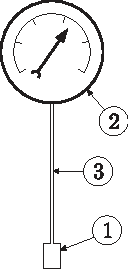
\includegraphics[width=0.25\linewidth]{2006-v2g-05-yl}
\end{center}
\fi
}

% Ü78
\ylDisplay{Tuulik} % Ülesande nimi
{Valter Kiisk} % Autor
{piirkonnavoor} % Voor
{2007} % Aasta
{G 5} % Ülesande nr.
{3} % Raskustase
{
% Teema: Gaasid
\ifStatement
Teatud tuuleturbiin (tiiviku diameeter $d = \SI{50}{m}$) töötab maksimaalse efektiivsusega tuule kiirusel $v = \SI{9}{m/s}$. Sel juhul õnnestub $\eta = \SI{40}{\%}$ tiiviku poolt haaratava õhuvoolu kineetilisest energiast muundada elektriks (kineetilise energia arvutamisel ei arvestata õhu pidurdumist tiivikul). Leidke nendel tingimustel tuuliku elektriline võimsus. Õhu tihedus on $\rho = \SI{1,3}{kg/m^3}$.
\fi
}

% Ü79
\ylDisplay{Rong tunnelis} % Ülesande nimi
{Eero Uustalu} % Autor
{lõppvoor} % Voor
{2009} % Aasta
{G 4} % Ülesande nr.
{3} % Raskustase
{
% Teema: Gaasid
\ifStatement
Rong liikus kiirusega $v=\SI{54}{km/h}$ läbi pika horisontaalse silindrikujulise tunneli.
Kui palju tõusis tunnelis asuva õhu temperatuur? Tunneli läbimõõt oli $d=\SI{5}{m}$.
Rongi elektrimootor tarbis tunnelit läbides võimsust $P=\SI{800}{kW}$.
Õhu molaarmass on $M=\SI{29}{g/mol}$, õhurõhk tunnelis $p=\SI{100}{kPa}$ ja algtemperatuur $t_0=\SI{17}{\celsius}$.
Õhk lugeda kaheaatomiliseks ideaalseks gaasiks. Eeldada, et rongi liikumisest tekkinud õhuvoolude liikumisest tulenev alarõhk on atmosfäärirõhuga võrreldes tühine\\
\emph{Märkus}. Kaheaatomilise gaasi siseenergia ühe molekuli kohta on $5/3$ korda suurem kui samal temperatuuril oleval üheaatomilisel gaasil.
\fi
}

% Ü80
\ylDisplay{Heelium} % Ülesande nimi
{Tundmatu autor} % Autor
{lahtine} % Voor
{2008} % Aasta
{G 6} % Ülesande nr.
{5} % Raskustase
{
% Teema: Gaasid
\ifStatement
Kolme mooli heeliumi soojendamisel muutus gaasi rõhk võrdeliselt gaasi ruumalaga. Mitme kraadi võrra tõusis heeliumi temperatuur, kui gaasile anti soojushulk $Q = \SI{300}{J}$?
\fi
}

% Ü81
\ylDisplay{Õhk} % Ülesande nimi
{Tundmatu autor} % Autor
{lahtine} % Voor
{2009} % Aasta
{G 7} % Ülesande nr.
{5} % Raskustase
{
% Teema: Gaasid
\ifStatement
Kaks anumat ruumalade suhtega $\alpha = V_1/V_2 = 2$ on ühendatud lühikese toruga, mille keskel asub ventiil. Ventiil laseb gaasi läbi juhul kui rõhkude vahe on suurem kui $\Delta p = 1,1p_0$, kus $p_0$ on atmosfäärirõhk. Temperatuuril $t_1 = \SI{27}{\celsius}$ on suuremas anumas õhk normaalrõhul, väiksemas anumas on vaakum. Milliseks kujuneb rõhk väiksemas anumas, kui mõlemad anumad soojendada temperatuurini $t_2 = \SI{127}{\celsius}$?
\fi
}

% Ü82
\ylDisplay{Õhuhoki} % Ülesande nimi
{Mihkel Heidelberg} % Autor
{lõppvoor} % Voor
{2010} % Aasta
{G 6} % Ülesande nr.
{5} % Raskustase
{
% Teema: Gaasid
\ifStatement
Heast soojusjuhist plaadile asetatakse kuivast jääst (st tahkest
süsihappegaasist) kerge seib raadiusega $r=\SI{1}{cm}$; seibi surutakse
pealt jõuga $F=\SI{10}{N}$. Millise minimaalse aluse
temperatuuri juures hõljub seib sublimeeruva süsihappegaasi tekitatud
gaasipadjal? Aluse temperatuur lugege ühtlaseks ja samaks temaga
vahetus kontaktis oleva ainekihiga. Õhurõhk $p_{0}=\SI{100}{kPa}$
ja kuiva jää aururõhu sõltuvus temperatuurist on kujutatud graafikul.

\begin{center}
	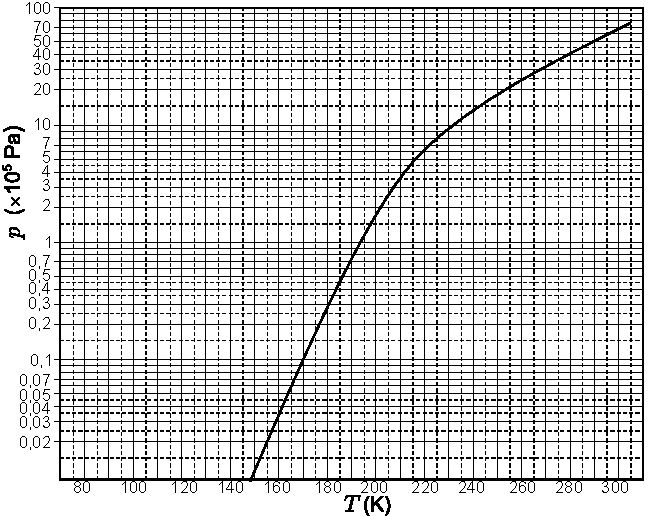
\includegraphics{2010-v3g-06-Aururohk}
\end{center}
\fi
}

% Ü83
\ylDisplay{Süstal} % Ülesande nimi
{Tundmatu autor} % Autor
{lahtine} % Voor
{2011} % Aasta
{G 5} % Ülesande nr.
{5} % Raskustase
{
% Teema: Gaasid
\ifStatement
Kord sooritas noor füüsik eksperimendi, et leida süstlakolvile mõjuvat
hõõrdejõudu. Ta tõmbas $V_{0}=\SI{10}{ml}$ mahuga süstlasse \SI{5,0}{ml} õhku ja sulges siis
süstla otsa sõrmega. Seejärel tõmbas ta süstla kolvi näiduni
$V_{1}=\SI{9,2}{ml}$ ja
lasi sellel seejärel aeglaselt tagasi liikuda. Kolb liikus, kuni näiduks jäi $V_{2}=\SI{5,8}{ml}$.
Mõõtmisel selgus, et süstlakolvi sisediameeter oli $d=\SI{9}{mm}$ ja kraadiklaas
näitas, et ruumis oli $t=\SI{27}{\celsius}$, õhu suhteline niiskus $R=30\%$ ja õhurõhk
$p_{0}=\SI{103,6}{kPa}$. Milline oli süstlakolvile mõjuv hõõrdejõud?\\
\textit{Märkus.} Kuna tegu on praktilise probleemiga, siis ei pruugi kõik
algandmed vajalikud olla.
\fi
}

% Ü84
\ylDisplay{Õhk} % Ülesande nimi
{Tundmatu autor} % Autor
{lahtine} % Voor
{2006} % Aasta
{G 8} % Ülesande nr.
{7} % Raskustase
{
% Teema: Gaasid
\ifStatement
Leida niiske (suhteline niiskus $f = \SI{90}{\%}$) ja kuiva õhu tiheduste suhe rõhu $p_0 = \SI{0,1}{MPa}$ ja temperatuuri $t = \SI{27}{\celsius}$ juures. Küllastunud auru tihedus sellel temperatuuril on $\rho_0 = \SI{0,027}{kg/m^3}$. Õhu molaarmass $\mu_1 = \SI{0,029}{kg/mol}$, vee molaarmass $\mu_2 = \SI{0,018}{kg/mol}$.
\fi
}

% Ü85
\ylDisplay{Gaasid} % Ülesande nimi
{Oleg Košik} % Autor
{lõppvoor} % Voor
{2007} % Aasta
{G 6} % Ülesande nr.
{7} % Raskustase
{
% Teema: Gaasid
\ifStatement
\begin{wrapfigure}[8]{r}{0.2\textwidth}
	\begin{center}
		\vspace{-20pt}
		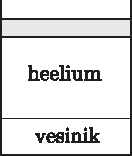
\includegraphics[width=0.95\linewidth]{2007-v3g-06-yl}
	\end{center}
\end{wrapfigure}
Isoleeritud silindrilises anumas vabalt liikuva koormise all on vesinik ja heelium, mis on teineteisest eraldatud vabalt liikuva ja aeglaselt soojust juhtiva õhukese vaheseinaga (vt. joonist). Alguses on gaaside temperatuurid võrdsed, kusjuures vesinik hõlmab heeliumist 3 korda väiksema ruumala. Vesinikule anti teatud soojushulk, mille tulemusena nihkus koormis $d_1 = \SI{5,5}{cm}$ võrra ülespoole. Pika aja möödudes täheldati, et koormis nihkus veel. Mis suunas ja kui palju see nihkus? Gaasid lugeda ideaalseteks. Vesiniku soojusmahtuvus konstantsel rõhul on $C\idx{PH_2} = 7R/2$ ning heeliumil $C\idx{PHe} = 5R/2$.
\fi
}

% Ü86
\ylDisplay{Korsten} % Ülesande nimi
{Jaan Kalda} % Autor
{piirkonnavoor} % Voor
{2009} % Aasta
{G 9} % Ülesande nr.
{7} % Raskustase
{
% Teema: Gaasid
\ifStatement
Hinnake, milline oleks suitsu kiirus korstnast väljumisel, kui õhutakistusega (sh turbulentsest liikumisest tingitud takistusega) korstnas ning ahjulõõrides võiks mitte arvestada.
Korstna kõrgus (mõõdetuna korstnajala juurest, kuhu siseneb ahjust tulev soe õhk) on $h=\SI{10}{m}$ ja õhu keskmine temperatuur korstnas $t=\SI{80}{\celsius}$. Lugeda, et ahju uks ja korstna jalg on samal kõrgusel. Välisõhu temperatuur on $t_0=\SI{0}{\celsius}$.
\fi
}

% Ü87
\ylDisplay{Rakettmootor} % Ülesande nimi
{Jaan Kalda} % Autor
{lahtine} % Voor
{2010} % Aasta
{G 10} % Ülesande nr.
{9} % Raskustase
{
% Teema: Gaasid
\ifStatement
\begin{wrapfigure}{r}{0.45\textwidth}
	\vspace{-3ex}
	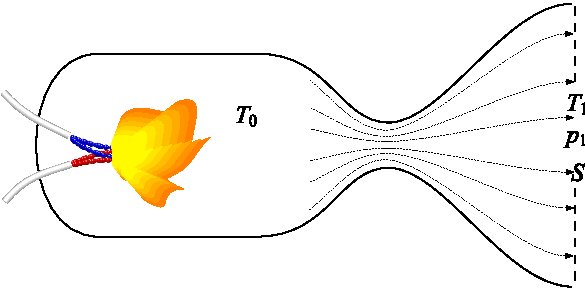
\includegraphics[width=\linewidth]{2010-lahg-10-rakettmootor}
	\vspace{-6ex}
\end{wrapfigure}
Vedelkütusel töötava rakettmootori skeem on toodud juuresoleval joonisel. Põlemiskambris moodustuvad põlemisproduktid (gaasid) omandavad kõrge rõhu ja temperatuuri. Seejärel väljuvad need adiabaatiliselt paisudes ja jahtudes läbi düüsi. Õigesti konstrueeritud düüsi korral (kaela läbimõõt vastab põlemiskiirusele ja -temperatuurile) jätkub adiabaatiline paisumine ka peale düüsikaela läbimist ning suur osa soojusenergiast muundatakse gaasijoa kineetiliseks energiaks. Leidke rakettmootori veojõud $F$ eeldusel, et (a) on teada düüsi väljundristlõike pindala $S$, temperatuur põlemiskambris $T_0$ ning gaaside temperatuur $T_1$ ja rõhk $p_1$ düüsist väljumise hetkel, kusjuures $T_0 \gg T_1$; (b) põlemiskambris on gaaside kineetiline energia tühine võrreldes soojusenergiaga; (c) atmosfäärirõhu mõju veojõule on tühine; (d) moodustuva gaasisegu ühe mooli soojusmahtuvus konstantsel ruumalal on $c_V = \frac52 R$, kus $R$ on gaasikonstant.
\fi
}
\newpage\subsection{\protect\StrSubstitute{Geomeetriline optika}{-}{ }}

% Ü88
\ylDisplay{Kiil} % Ülesande nimi
{Valter Kiisk} % Autor
{lõppvoor} % Voor
{2007} % Aasta
{G 3} % Ülesande nr.
{2} % Raskustase
{
% Teema: Geomeetriline optika
\ifStatement
Laserkiire teele asetatakse enam-vähem risti õhuke klaasplaat (klaasi murdumisnäitaja $n = \num{1,5}$). Selle tulemusena nihkub $L = \SI{2}{m}$ kaugusel ekraanil olev laserkiire kujutis $d = \SI{5}{mm}$ võrra. Järeldatakse, et plaat on kergelt kiilukujuline. Leidke selle kiilu tipunurk $\alpha$. 

\emph{Vihje}. Väikeste nurkade $\varphi$ puhul $\sin \varphi \approx \tan \varphi \approx \varphi$.
\fi
}

% Ü89
\ylDisplay{Lääts} % Ülesande nimi
{Tundmatu autor} % Autor
{lahtine} % Voor
{2009} % Aasta
{G 2} % Ülesande nr.
{2} % Raskustase
{
% Teema: Geomeetriline optika
\ifStatement
Lääts tekitab esemest $d = \SI{24}{cm}$ kaugusele ekraanile kujutise, mis on esemest \num{3} korda suurem. Leidke läätse fookuskaugus.
\fi
}

% Ü90
\ylDisplay{Kiirtekimbu laiendi} % Ülesande nimi
{Koit Timpmann} % Autor
{piirkonnavoor} % Voor
{2010} % Aasta
{G 3} % Ülesande nr.
{2} % Raskustase
{
% Teema: Geomeetriline optika
\ifStatement
Kaks ühise optilise peateljega läätse moodustavad seadme, millega saab paralleelsest valgusvihust moodustada esialgsest laiema või kitsama paralleelse valgusvihu. Kasutatava seadme esimese läätse optiline tugevus on \SI{-20}{dpt}. Kui kaugele esimesest läätsest tuleks paigutada teine lääts, et laiendada seadmele langev valgusvihk \num{2.5}-kordseks?
\fi
}

% Ü91
\ylDisplay{Nõguspeegel} % Ülesande nimi
{EFO žürii} % Autor
{lõppvoor} % Voor
{2006} % Aasta
{G 2} % Ülesande nr.
{3} % Raskustase
{
% Teema: Geomeetriline optika
\ifStatement
On teada esemelt lähtunud ühe kiire suund enne ja pärast peegeldumist sfääriliselt nõguspeeglilt. Teades eseme $AB$ ja optilise peatelje asukohta, konstrueerige eseme kujutis ja tähistage nõguspeegli fookuse asukoht. Ignoreerida sfäärilisi aberratsioone.

\begin{center}
	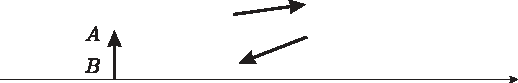
\includegraphics[width=0.9\linewidth]{2006-v3g-02-yl}
\end{center}
\fi
}

% Ü92
\ylDisplay{Plaat} % Ülesande nimi
{Tundmatu autor} % Autor
{lahtine} % Voor
{2007} % Aasta
{G 4} % Ülesande nr.
{3} % Raskustase
{
% Teema: Geomeetriline optika
\ifStatement
Tasaparalleelsel plaadil paksusega $d = \SI{5}{cm}$ on alumine pind hõbetatud. Valguskiir langeb plaadi ülemisele pinnale nurga $\alpha = \SI{30}{\degree}$ all, osaliselt peegeldub sellelt ning osaliselt murdub plaadi sisse. Seejärel peegeldub murdunud kiir plaadi alumiselt pinnalt ning murdub teist korda, väljudes tagasi õhku. Leidke plaadi materjali murdumistegur $n$, kui kaugus esimese peegeldunud ja teise murdunud kiirte vahel $l = \SI{2,5}{cm}$.
\fi
}

% Ü93
\ylDisplay{Valgusvihk} % Ülesande nimi
{Mihkel Kree} % Autor
{piirkonnavoor} % Voor
{2005} % Aasta
{G 5} % Ülesande nr.
{4} % Raskustase
{
% Teema: Geomeetriline optika
\ifStatement
On antud ülesanne muuta kitsas paralleelne valgusvihk võimalikult laiaks paralleelseks valgusvihuks. Kasutada saab vaid kahte läätse etteantud kolmest: kumerlääts (fookuskaugus $f_1 = \SI{20}{cm}$), kumerlääts ($f_2 = \SI{40}{cm}$) ning nõguslääts ($f_3 = \SI{-10}{cm}$). Kuidas tuleb toimida ning mitu korda laiemaks valgusvihk sel juhul muutub? Eeldage, et läätsede mõõtmed on oluliselt suuremad valgusvihu laiusest.
\fi
}

% Ü94
\ylDisplay{Biprisma} % Ülesande nimi
{Mihkel Kree} % Autor
{piirkonnavoor} % Voor
{2006} % Aasta
{G 6} % Ülesande nr.
{4} % Raskustase
{
% Teema: Geomeetriline optika
\ifStatement
Paralleelne kiirtekimp langeb võrdhaarsele kolmnurksele prismale risti prisma tahuga (vt joonist). Prisma teravnurgad on väikesed, suurusega $\alpha$. Prisma materjali murdumisnäitaja on $n$. Prismast kaugusel $d$ paikneb koondav lääts fookuskaugusega $f$. Läätse optiline peatelg on paralleelne kiirtekimbu esialgse sihiga ning läbib prisma tipunurka. Missugune pilt tekib läätse fokaaltasandis asuvale ekraanile? Leida pilti iseloomustavad parameetrid. Kuidas sõltub pilt kaugusest $d$? 

\emph{Märkus}. Väikeste nurkade korral kehtib lähendus $\tan \alpha \approx \sin \alpha \approx \alpha$.

\begin{center}
	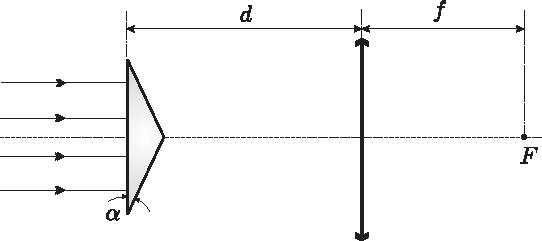
\includegraphics[width=\linewidth]{2006-v2g-06-yl}
\end{center}
\fi
}

% Ü95
\ylDisplay{Varjud} % Ülesande nimi
{Jaak Kikas} % Autor
{piirkonnavoor} % Voor
{2007} % Aasta
{G 6} % Ülesande nr.
{4} % Raskustase
{
% Teema: Geomeetriline optika
\ifStatement
Läbipaistmatut kera valgustab kerakujuline valgusallikas. Joonisele on kantud läbipaistmatu kera poolt tekitatud täis- ja poolvarju koonuste lõiked joonise tasandiga (kera keskpunkt asub samas tasandis). Konstrueerige valgusallika lõige joonise tasandiga. Valgusallika keskpunkt asetseb samuti joonise tasandis.

\begin{center}
	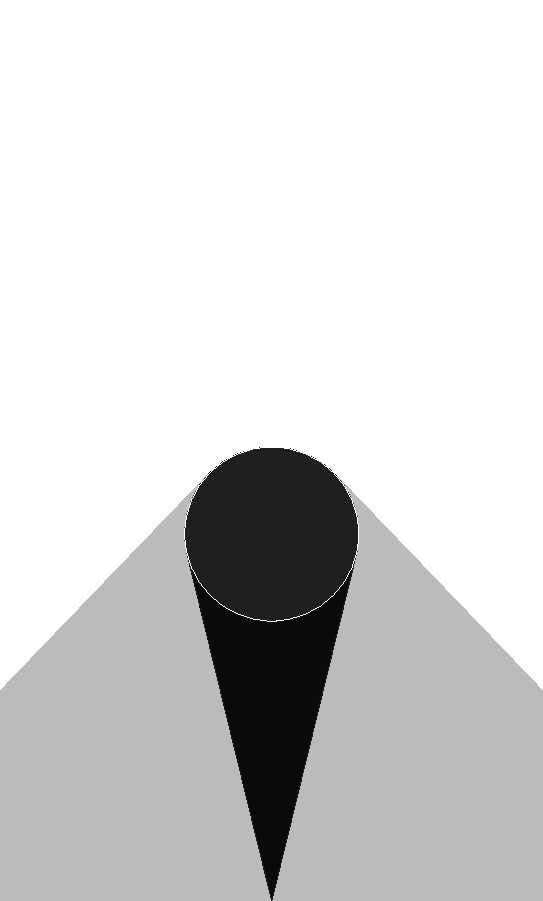
\includegraphics[height=0.8\textheight]{2007-v2g-06-yl}
\end{center}
\fi
}

% Ü96
\ylDisplay{Veealune valgus} % Ülesande nimi
{Jaak Kikas} % Autor
{lõppvoor} % Voor
{2008} % Aasta
{G 5} % Ülesande nr.
{4} % Raskustase
{
% Teema: Geomeetriline optika
\ifStatement
Kas basseini kohal rippuv punktvalgusallikas, mida vaadeldakse basseini põhjast, on heledam siis, kui bassein on veest tühi, või siis, kui ta on veega täidetud ja kaugus silmast veepinnani võrdub valgusallika kõrgusega veepinna kohal? Mitu korda? Veepinnalt peegeldub tagasi $r = \SI{2}{\%}$ valgust, vee murdumisnäitaja on $n = \num{1,33}$ ja neeldumine vees on tühine. Allika heledus on võrdeline silmaavasse sattuva valguse energiaga, silmaava läbimõõdu loeme samaks kõigis vaatlustingimustes ja väikeseks võrreldes vaatleja sügavusega.
\fi
}

% Ü97
\ylDisplay{Konfokaalne mikroskoop} % Ülesande nimi
{Mihkel Rähn} % Autor
{lõppvoor} % Voor
{2009} % Aasta
{G 7} % Ülesande nr.
{4} % Raskustase
{
% Teema: Geomeetriline optika
\ifStatement
Harilikest mikroskoopidest parema ruumilise lahutuse saamiseks kasutatakse konfokaalseid
mikroskoope. Juuresoleval joonisel on kujutatud konfokaalse mikroskoobi põhielemendid:
objektiiv, läätsed L$_1$ ja L$_2$ ning nende ühises fokaaltasandis asuv väike ringikujuline ava.
Joonisel on samuti esitatud optilisel peateljel asuvast väikesest uuritavast esemest lähtuvate
kiirte käik.
Objektiivi fokaaltasandist kaugemal ja lähemal olevatest
objektidest lähtuvad kiired ei läbi enamuses ava, vaid neelduvad ava servadel.
Kõrvalnähtusena vaateväli kitseneb. Kui kaugel optilisest peateljest
võib olla objektiivi fokaaltasandis olev ese, et see oleks veel nähtav? Läätsede L$_1$, L$_2$ ja objektiivi fookuskaugused on vastavalt $f_1$, $f_2$ ja $f_{\mathrm{obj}}$, ava läbimõõt $d$.

\begin{center}
	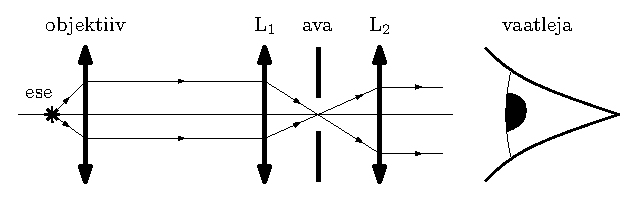
\includegraphics[width=0.8\linewidth]{2009-v3g-07-G_konfokaalne_mikroskoop.eps}
\end{center}
\fi
}

% Ü98
\ylDisplay{Klaaskuulike} % Ülesande nimi
{Jaan Kalda} % Autor
{lahtine} % Voor
{2010} % Aasta
{G 4} % Ülesande nr.
{4} % Raskustase
{
% Teema: Geomeetriline optika
\ifStatement
Paljudes helkurmaterjalides kasutatakse valguse tagasisuunamiseks tillukesi
klaaskuulikesi, mis kantakse tiheda kihina materjali pinnale. Uurigem, milline
peaks olema selliste klaaskuulikeste murdumisnäitaja. Teeme järgmised eeldused:
(a) klaaskuulile langeb valguskiir nii, et valguskiire ja pinnanormaali vaheline
nurk $\alpha$ on väike ($\alpha \ll \SI{1}{rad}$); (b) valguskiir murdub klaasi
pinnal, peegeldub ühekordselt kuuli sisepinnalt ja väljub seejärel kuulist
(murdudes teistkordselt kuuli pinnal). Millise murdumisnäitaja $n$ korral
suundub selline valguskiir täpselt tagasi? Tehke kiirtekäigu joonis ja
põhjendage vastust. \emph{Abivalem:} väikese $\alpha$ korral radiaanmõõdus
$\sin\alpha \approx \alpha$.
\fi
}

% Ü99
\ylDisplay{Kiilud} % Ülesande nimi
{Tundmatu autor} % Autor
{lahtine} % Voor
{2006} % Aasta
{G 6} % Ülesande nr.
{5} % Raskustase
{
% Teema: Geomeetriline optika
\ifStatement
Tasaparalleelne plaat koosneb kahest klaaskiilust väikse nurgaga $\varphi \ll 1$ (vt joonist). Kiilude murdumisnäitajad on $n_1$ ja $n_2$ ($n_2 > n_1$). Plaadile risti tema pinnaga langeb paralleelne valgusvihk. Plaadi taga asub koondav lääts fookuskaugusega $f$. Läätse fokaaltasandis asub ekraan. Joonistage kiirte käik süsteemis. Kui palju nihkub valguslaik ekraanil, kui me eemaldame plaadi? 

\emph{Vihje}. Väikeste nurkade puhul kehtib ligikaudne võrdus $\tan \varphi \approx \sin \varphi \approx \varphi $.

\begin{center}
	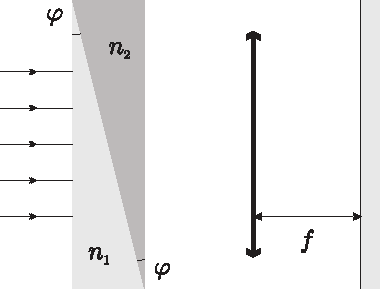
\includegraphics[width=0.6\linewidth]{2006-lahg-06-yl}
\end{center}
\fi
}

% Ü100
\ylDisplay{Klaaskuup} % Ülesande nimi
{Tundmatu autor} % Autor
{piirkonnavoor} % Voor
{2009} % Aasta
{G 7} % Ülesande nr.
{5} % Raskustase
{
% Teema: Geomeetriline optika
\ifStatement
Klaaskuubi neli tahku on värvitud mustaks nõnda,
et värvimata jäänud tahud paiknevad kõrvuti (omavad ühist serva). Missugune peab olema klaasi murdumisnäitaja $n$, et ka värvimata tahud
paistaksid mustadena?
\fi
}

% Ü101
\ylDisplay{Peeglid} % Ülesande nimi
{Jaan Kalda} % Autor
{piirkonnavoor} % Voor
{2009} % Aasta
{G 8} % Ülesande nr.
{5} % Raskustase
{
% Teema: Geomeetriline optika
\ifStatement
Kui paigutada kaks tasapeeglit nii, et nende tasapinnad moodustavad nurga $\alpha<180^\circ$ ning peegeldavad pinnad on vastamisi, siis peeglite vahele paigutatud asjadest võib tekkida mitu kujutist: lisaks peegeldustele veel peegelduse-peegeldused jne. Joonisel on kujutatud valgusallika $S$ kaks peegeldust ning üks peegelduse-peegeldus ülaltvaates (st peeglite tasapindade lõikejoone sihis). Leida konstruktsiooni abil peeglite ning valgusallika asukohad.\\

\begin{center}
	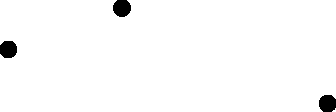
\includegraphics[width=0.6\linewidth]{2009-v2g-08-yl}
\end{center}
\fi
}

% Ü102
\ylDisplay{Kapillaartoru} % Ülesande nimi
{Tundmatu autor} % Autor
{lahtine} % Voor
{2009} % Aasta
{G 8} % Ülesande nr.
{6} % Raskustase
{
% Teema: Geomeetriline optika
\ifStatement
Klaasist kapillaartoru on sisemise raadiusega $r$ ja välimise raadiusega $R$. Millist tingimust peavad rahuldama $r$, $R$ ja klaasi murdumisnäitaja $n$, et küljelt vaadates paistaks, et kapillaartoru seinapaksus on null?
\fi
}

% Ü103
\ylDisplay{Lääts} % Ülesande nimi
{Tundmatu autor} % Autor
{lahtine} % Voor
{2007} % Aasta
{G 9} % Ülesande nr.
{7} % Raskustase
{
% Teema: Geomeetriline optika
\ifStatement
Teritamata pliiatsi telg ühtib koondava läätse peateljega. Mitu korda on pliiatsi kujutise pikkus tema enda pikkusest erinev, kui pliiatsi ühe otsa kujutise diameetri ja pliiatsi diameetri suhe on $k_1$ ning teise otsa jaoks on see suhe $k_2$? Pliiatsi mõlemad otsad asuvad läätsest fookuskaugusest suuremal kaugusel.
\fi
}

% Ü104
\ylDisplay{Hajuti} % Ülesande nimi
{Andreas Valdmann} % Autor
{piirkonnavoor} % Voor
{2010} % Aasta
{G 8} % Ülesande nr.
{7} % Raskustase
{
% Teema: Geomeetriline optika
\ifStatement
Mõnedes valgustites kasutatakse valguse hajutamiseks joonisel kujutatud ristlõikega
pleksiklaasist plaati. Valgus langeb selle siledale poolele ja läbib hajuti vaid juhul, kui
langemisnurk on suurem kriitilisest nurgast $\alpha_\mathrm{kr}$. Leidke nurga $\alpha_\mathrm{kr}$ väärtus. Pleksiklaasi
murdumisnäitaja $n=\num{1,5}$. Kõik sakilise poole tahud on \num{45}-kraadise nurga all sileda poole pinna
suhtes.
\begin{center}
	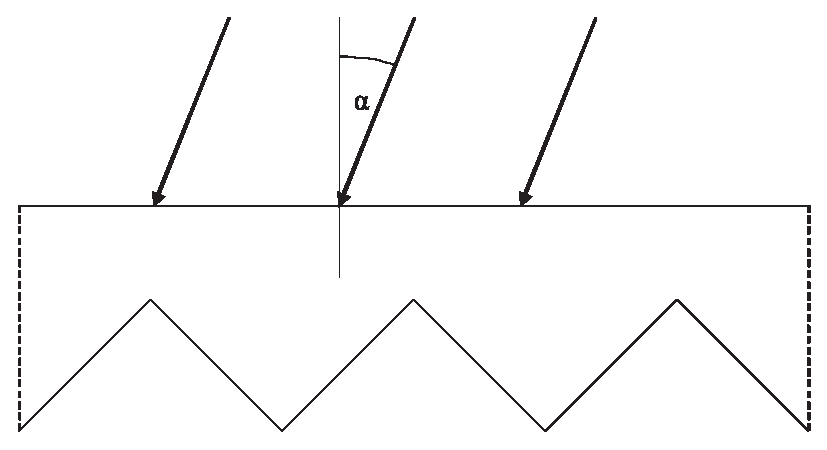
\includegraphics[width=0.475\textwidth]{2010-v2g-08-hajuti.eps}
\end{center}
\fi
}

% Ü105
\ylDisplay{Nõguslääts eestvaates} % Ülesande nimi
{Siim Ainsaar} % Autor
{piirkonnavoor} % Voor
{2011} % Aasta
{G 10} % Ülesande nr.
{7} % Raskustase
{
% Teema: Geomeetriline optika
\ifStatement
Joonisel on kujutatud eestvaates nõguslääts, mille optiline peatelg on joonise tasandiga risti ja lõikub läätsega punktis $O$. Antud on ka üks horisontaalne valguskiir ning selle lõikepunktid eesmise fokaaltasandi ning läätsega (vastavalt punktid $K$ ja $L$). Joonestage antud vaates lisalehel kiire edasine käik ning ta lõikepunkt tagumise fokaaltasandiga. Põhjendage lahendust.
\begin{center}
	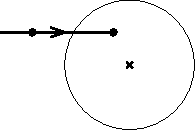
\includegraphics[width=0.5\linewidth]{2011-v2g-10-yl}
\end{center}
\fi
}

% Ü106
\ylDisplay{Gravitatsioonilääts} % Ülesande nimi
{Mihkel Kree} % Autor
{piirkonnavoor} % Voor
{2007} % Aasta
{G 10} % Ülesande nr.
{8} % Raskustase
{
% Teema: Geomeetriline optika
\ifStatement
Üldrelatiivsusteooria ennustab, et mustast august möödumisel kaldub valguskiir gravitatsiooni tõttu kõrvale oma esialgsest liikumissuunast nurga $\varphi = 4GM/c^2r$ võrra, kus $M$ on musta augu mass ning $r$ trajektoori lähima punkti kaugus selleni. Sattugu must auk täpselt vaatleja ja tähe vahele, nii et kaugus vaatlejast musta auguni on $L_1$ ning mustast august täheni $L_2$. Missugune on tähe kujutis vaatleja jaoks (põhjendage oma vastust kiirte käigu visandi abil) ning kui suur on kujutise nurkläbimõõt? Kuna vaatlejani jõudvate kiirte jaoks on $r$ palju väiksem tähe kaugusest, võib kasutada väikeste nurkade lähendust $\sin \alpha \approx \tan \alpha \approx \alpha$.
\fi
}

% Ü107
\ylDisplay{Kuup} % Ülesande nimi
{Jaan Kalda} % Autor
{lõppvoor} % Voor
{2007} % Aasta
{G 8} % Ülesande nr.
{8} % Raskustase
{
% Teema: Geomeetriline optika
\ifStatement
\begin{wrapfigure}[16]{r}{0.5\textwidth}
	\begin{center}
		\vspace{-20pt}
		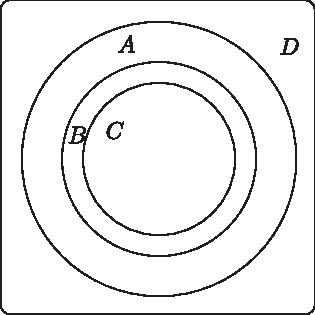
\includegraphics[width=0.95\linewidth]{2007-v3g-08-yl}
	\end{center}
\end{wrapfigure}
Läbipaistvast klaasist tehtud kuubis on suur kerakujuline õõnsus, mis on täidetud sinist värvi gaasiga. Kuup lebab kollaste seintega toas valgel põrandal. Juuresolev kuubi joonis on tehtud kuubi kohalt pildistatud foto põhjal, millelt on eemaldatud kõik värvid ning jäetud alles selgeltnähtavad kontuurid ja erivärviliste piirkondade eraldusjooned (joonte kujud ja mõõtmed on täpselt sellised nagu fotol). Kuubi mõõtmed lugeda hulga väiksemateks põranda mõõtmetest ning kõrgusest, millelt on tehtud joonise aluseks olnud foto. Millistele värvidele vastavad tähed $A$, $B$, $C$, $D$? Põhjendage vastust. Leidke klaasi murdumisnäitaja.
\fi
}

% Ü108
\ylDisplay{Akvaarium} % Ülesande nimi
{Tundmatu autor} % Autor
{lahtine} % Voor
{2005} % Aasta
{G 10} % Ülesande nr.
{9} % Raskustase
{
% Teema: Geomeetriline optika
\ifStatement
Leidke maksimaalne suurendus $k$, mille tekitab sfääriline akvaarium, kui vaadata väljastpoolt selles ujuvat kala. Suurenduse all mõistame siin kala kujutise ja tegeliku kala suuruste suhet. Vee murdumisnäitaja $n = \num{1,3}$. Väikeste nurkade puhul kehtib ligikaudne võrdus $\sin \alpha \approx \alpha$. 
\fi
}

% Ü109
\ylDisplay{Nõguspeegel} % Ülesande nimi
{Mihkel Kree} % Autor
{lõppvoor} % Voor
{2007} % Aasta
{G 9} % Ülesande nr.
{9} % Raskustase
{
% Teema: Geomeetriline optika
\ifStatement
Optiline süsteem koosneb kumerläätsest ja nõguspeeglist, mille optilised peateljed ühtivad. Kumerpeegli asukohta pole joonisel märgitud. On teada, et objektist $A$ tekib teisele poole läätse kaks kujutist $K_1$ ja $K_2$. Konstrueerige kumerpeegli kõveruskeskpunkt $O$ ja kumerpeeglis objektist $A$ tekkinud näiv kujutis $A'$. Eeldada, et optilises süsteemis on nurgad piisavalt väiksed, et sfäärilisi aberratsioone ei teki.

\begin{center}
	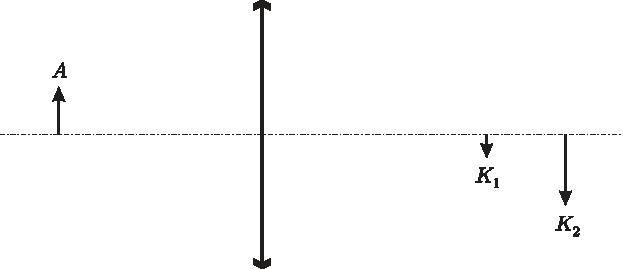
\includegraphics[width=\linewidth]{2007-v3g-09-yl}
\end{center}
\fi
}

% Ü110
\ylDisplay{Kärbes} % Ülesande nimi
{Aigar Vaigu} % Autor
{piirkonnavoor} % Voor
{2008} % Aasta
{G 10} % Ülesande nr.
{9} % Raskustase
{
% Teema: Geomeetriline optika
\ifStatement
Kärbes on merevaigutükis, mille murdumisnäitaja on $n=\num{1,6}$. Tüki üks pinnaosa on sfääriline kõverusraadiusega $r = \SI{3}{mm}$. Kui vaadata kärbse pead läbi selle pinnaosa, siis näib pea asuvat kõveruskeskpunkti läbival sirgel $k = \SI{5}{mm}$ sügavusel merevaigus. Kui sügaval on kärbse pea tegelikult? 

\emph{Märkus}. Kasutada väikeste nurkade lähendust $\tan \alpha \approx \sin \alpha \approx \alpha$, kus $\alpha \gg 1$ on väike nurk mõõdetuna radiaanides.
\fi
}

% Ü111
\ylDisplay{Punktallikad} % Ülesande nimi
{Jaan Kalda} % Autor
{lõppvoor} % Voor
{2010} % Aasta
{G 9} % Ülesande nr.
{9} % Raskustase
{
% Teema: Geomeetriline optika
\ifStatement
Juuresoleval joonisel on neli punkti, millest kaks on valgusallikad ja kaks nende tõelised kujutised, mille on tekitanud õhuke lääts. Leidke konstrueerimise teel läätse tasand ja optiline peatelg. Kui võimalusi on rohkem kui üks, siis leidke need kõik.

\begin{center}
	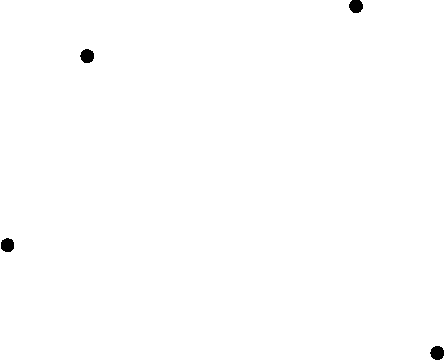
\includegraphics[width=0.3\linewidth]{2010-v3g-09-punktid}
\end{center}
\fi
}

% Ü112
\ylDisplay{Optiline süsteem} % Ülesande nimi
{Andreas Valdmann} % Autor
{lõppvoor} % Voor
{2011} % Aasta
{G 8} % Ülesande nr.
{9} % Raskustase
{
% Teema: Geomeetriline optika
\ifStatement
Klaasist murdumisnäitajaga $n$ on valmistatud õhuke kaksikkumer lääts, mille mõlema pinna kõverusraadius on $r$ (läätse paksus
$d \gg r$). Läätse üks pind kaetakse peegeldava metallikihiga. Leidke kumerläätsest ja nõguspeeglist tekkinud optilise süsteemi fookuskaugus. 

\emph{Vihje}. Fookuskauguse leidmiseks võib vaadelda optilise peatelje lähedasi kiiri, mis levivad
selle suhtes väikese nurga all. Sel juhul saab rakendada väikeste nurkade valemit $\sin \alpha \approx \tan \alpha \approx \alpha$, kus $\alpha$ on radiaanides. 
\fi
}

% Ü113
\ylDisplay{Sähvatus} % Ülesande nimi
{Mihkel Kree} % Autor
{lõppvoor} % Voor
{2006} % Aasta
{G 9} % Ülesande nr.
{10} % Raskustase
{
% Teema: Geomeetriline optika
\ifStatement
Optiline süsteem koosneb kahest nõguspeeglist ja kumerläätsest (vt joonist), mille optilised peateljed ühtivad. Ringikujulise ristlõikega valgusimpulss siseneb süsteemi optilise peatelje sihis ning valgusvihu telg ühtib sellega. Peeglite kõverusraadiused on $R_1 = \SI{8}{m}$ ja $R_2 = \SI{4}{m}$ ning peeglite vahekaugus $L = \SI{6}{m}$. Peeglite läbimõõdud on $d_1 = \SI{160}{mm}$ ja $d_2 = \SI{96}{mm}$. Kiire läbimõõt on $D = \SI{192}{mm}$. Läätse läbimõõt on suurem valgusvihu omast. Suurema peegli keskel on ava läbimõõduga $d_0 = \SI{1}{mm}$. Joonistage valguse intensiivsuse ajaline kulg kumerläätse fookuses $f$. Eeldage, et süsteemi saabuva impulsi kestvus $\tau \ll L/c$. Valguse kiirus $c = \SI{3e8}{m/s}$.

\begin{center}
	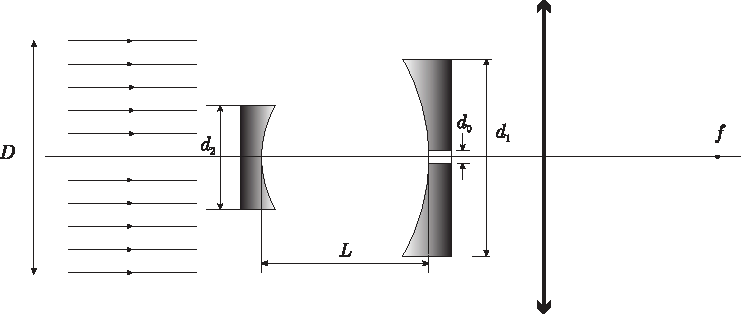
\includegraphics[width=0.95\linewidth]{2006-v3g-09-yl}
\end{center}
\fi
}
\newpage\subsection{\protect\StrSubstitute{Kinemaatika}{-}{ }}

% Ü114
\ylDisplay{Autod} % Ülesande nimi
{Oleg Košik} % Autor
{piirkonnavoor} % Voor
{2006} % Aasta
{G 1} % Ülesande nr.
{1} % Raskustase
{
% Teema: Kinemaatika
\ifStatement
Tartu ja Tallinna vahemaa on $s = \SI{180}{km}$. Jalgrattur sõidab Tartust Tallinna poole kiirusega $v_1 = \SI{30}{km/h}$. Sõites luges ta kokku, et $t_0 = \SI{5}{min}$ jooksul tuli talle vastu $n_0 = \SI{20}{autot}$. Mitu Tallinnast Tartusse sõitvat autot on korraga maanteel? Eeldada, et autod sõidavad võrdsete vahemaadega kiirusega $v_2 = \SI{90}{km/h}$ kogu maantee ulatuses.
\fi
}

% Ü115
\ylDisplay{Auto} % Ülesande nimi
{Tundmatu autor} % Autor
{lahtine} % Voor
{2008} % Aasta
{G 1} % Ülesande nr.
{1} % Raskustase
{
% Teema: Kinemaatika
\ifStatement
Paigalseisust liikuma hakanud autol kulus teatud vahemaa läbimiseks $t = \SI{15}{s}$. Millise ajaga läbis auto viimase viiendiku sellest vahemaast? Auto liikumine lugeda ühtlaselt kiirenevaks.
\fi
}

% Ü116
\ylDisplay{Ratturid} % Ülesande nimi
{Tundmatu autor} % Autor
{lahtine} % Voor
{2009} % Aasta
{G 1} % Ülesande nr.
{1} % Raskustase
{
% Teema: Kinemaatika
\ifStatement
Kolm ratturit sõitsid linnast $A$ linna $B$. Linnast $A$ väljusid nad üheaegselt. Esimese ratturi keskmine kiirus oli $v_1 = \SI{30}{km/h}$, teise ratturi oma $v_2 = \SI{20}{km/h}$. Esimene rattur jõudis sihtpunkti kell 19.00, teine rattur kell 20.00 ning kolmas rattur kell 21.00. Milline oli kolmanda ratturi keskmine kiirus $v_3$?
\fi
}

% Ü117
\ylDisplay{Veok} % Ülesande nimi
{Valter Kiisk} % Autor
{piirkonnavoor} % Voor
{2005} % Aasta
{G 1} % Ülesande nr.
{2} % Raskustase
{
% Teema: Kinemaatika
\ifStatement
Veok sõidab maanteel ühtlase kiirusega $v_1 = \SI{80}{km/h}$. Veokile järgneb $l_1 = \SI{10}{m}$ kaugusel sõiduauto. Veoki pikkus on $L_1 = \SI{12}{m}$, sõiduauto pikkus $L_2 = \SI{4}{m}$. Sõiduauto sooritab möödasõidu ühtlase kiirendusega $a = \SI{2}{m/s^2}$. Möödasõit lõpeb siis, kui sõiduauto on veokist $l_2 = \SI{10}{m}$ kaugusel. Kui pikas minimaalses ulatuses $s$ peaks vastassuunaline rada vaba olema ohutuks möödasõiduks? Ohutuks kauguseks vastutulevast autost loetakse $l_3 = \SI{30}{m}$. Vastutulevad autod sõidavad kiirusega $v_2 = \SI{90}{km/h}$.

\begin{center}
	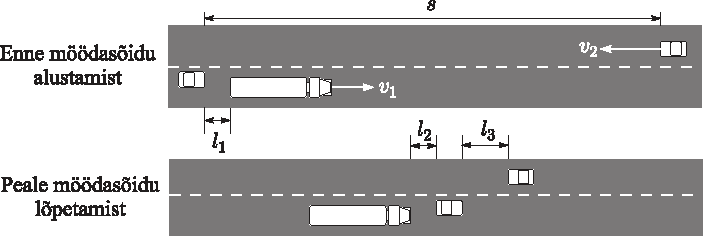
\includegraphics[width=\linewidth]{2005-v2g-01-yl}
\end{center}
\fi
}

% Ü118
\ylDisplay{Rongiõnnetus} % Ülesande nimi
{Oleg Košik} % Autor
{piirkonnavoor} % Voor
{2011} % Aasta
{G 4} % Ülesande nr.
{2} % Raskustase
{
% Teema: Kinemaatika
\ifStatement
Kehrast Aegviidu poole sõitis kiirusega $v_1=\SI{63}{km/h}$ kaubarong. Aegviidust hakkas sama teed pidi sõitma Kehra poole elektrirong kiirendusega $a_2=\SI{0,15}{m/s^2}$. Kui rongide vahemaa oli $s=\SI{2750}{m}$, märkas kaubarongi vedurijuht vastusõitvat elektrirongi ning vajutas pidurile. Elektrirongi kiirus oli selleks hetkeks $v_2=\SI{18}{km/h}$. Leidke rongide sõidukiirused vahetult kokkupõrke eel. Kaubarongi pidudrdukiirendus on $a_1=-\SI{0,1}{m/s^2}$.
\fi
}

% Ü119
\ylDisplay{Sonar} % Ülesande nimi
{Oleg Košik} % Autor
{piirkonnavoor} % Voor
{2006} % Aasta
{G 3} % Ülesande nr.
{3} % Raskustase
{
% Teema: Kinemaatika
\ifStatement
Vaatame järgmist meetodit laeva kiiruse määramiseks. Saadame rannikult sellest eemalduvale laevale ultraheli signaali sagedusega $f_1$. Laevalt peegeldub signaal tagasi rannikule, kus vastuvõtja fikseerib signaali sagedusega $f_2$. Teades, et heli kiirus õhus on $v_h$, määrake laeva kiirus $v$.
\fi
}

% Ü120
\ylDisplay{Autod} % Ülesande nimi
{Jaan Kalda} % Autor
{piirkonnavoor} % Voor
{2008} % Aasta
{G 2} % Ülesande nr.
{3} % Raskustase
{
% Teema: Kinemaatika
\ifStatement
Juuresolev joonis on tehtud kõrgelt otse alla pildistatud foto põhjal, millel on jäädvustatud kaks autot (tähistatud punktidega $A$ ja $B$), mis lähenevad ristmikule jäävate kiirustega $v_A = \SI{40}{km/h}$ ja $v_B = \SI{60}{km/h}$. Kasutades joonist ja sellel antud mõõtkava, leidke autode edasisel liikumisel nende vaheline minimaalne kaugus.

\begin{center}
	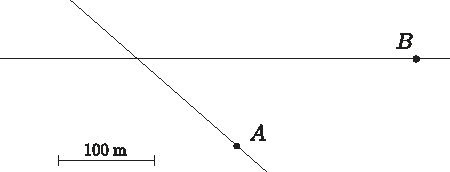
\includegraphics[width=0.9\linewidth]{2008-v2g-02-yl}
\end{center}
\fi
}

% Ü121
\ylDisplay{GPS} % Ülesande nimi
{Jaan Kalda} % Autor
{lõppvoor} % Voor
{2009} % Aasta
{G 5} % Ülesande nr.
{4} % Raskustase
{
% Teema: Kinemaatika
\ifStatement
Tervisesportlane kasutab GPS seadet oma jooksutreeningu tulemuste salvestamiseks.
Tema GPS seade määrab iga 15 sekundi järel jooksja täpse asukoha, mille põhjal arvutab ja salvestab GPS seade viimase 15 sekundi keskmise kiiruse.
GPS esitab saadud tulemused graafikul punktidena, mis on ühendatud sirglõikude abil.
Jooksja märkas, et ketsipael oli lahti läinud.
Ta peatus, sidus selle kinni ning tänu väikesele puhkusele jätkas jooksu juba natuke suurema
kiirusega, vt juuresolevat GPS-i esitatud graafikut. Kui kaua kestis peatus? Pidurdumiseks ning puhkusjärgselt kiirendamiseks kulunud
aeg lugeda tühiseks; jooksu kiirus oli konstantne nii enne peatust kui ka pärast seda.

\begin{center}
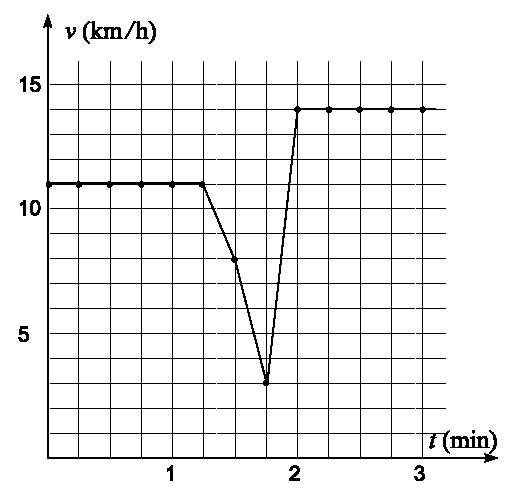
\includegraphics{2009-v3g-05-gps.eps}
\end{center}
\fi
}

% Ü122
\ylDisplay{Tsunami} % Ülesande nimi
{Jaan Kalda} % Autor
{lõppvoor} % Voor
{2005} % Aasta
{G 6} % Ülesande nr.
{6} % Raskustase
{
% Teema: Kinemaatika
\ifStatement
\begin{wrapfigure}[10]{r}{0.45\textwidth}
	\begin{center}
		\vspace{-20pt}
		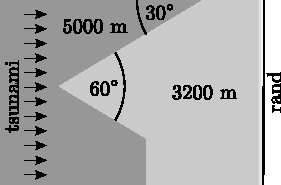
\includegraphics[width=\linewidth]{2005-v3g-06-yl}
	\end{center}
\end{wrapfigure}

Joonisel on toodud ookeanipõhja sügavus kodeeritud halltoonidega: tumedam hall vastab sügavamale, heledam hall madalamale veele. Ookeanipõhjas on astang, kus $h_1 = \SI{5000}{m}$ sügavune vesi läheb $h_2 = \SI{3200}{m}$ sügavuseks; ranna lähedal toimub madaldumine väga kiiresti. Rannale läheneb tsunami nii, nagu näidatud joonisel. Tsunami liikumiskiirus $v = \sqrt{gh}$, kus $g = \SI{9,8}{m/s^2}$ ja $h$ tähistab vee sügavust. Millisesse ranna punkti jõuab kõige kõrgem laine? Põhjendage vastust.
\fi
}

% Ü123
\ylDisplay{Hävituslennuk} % Ülesande nimi
{Tundmatu autor} % Autor
{lahtine} % Voor
{2011} % Aasta
{G 7} % Ülesande nr.
{6} % Raskustase
{
% Teema: Kinemaatika
\ifStatement
Ühel ilusal augustipäeval käis Mati paraadil vaatamas NATO hävituslennukeid, mis
tegid üle rahva peade demonstratsioonlende. Diktor ütles valjuhääldist, et lennuk
lendab horisontaalselt üle rahva kiirusega $v=\SI{1350}{km/h}$. Matit huvitas aga, kui
kõrgel lennuk lendab. Vajalike mõõtetulemuste saamiseks seisis ta nii, et tema
ja läheneva lennukiga ühele joonele jäi täpselt üks 9 meetri pikkune elektripost
ning Mati ise asus teise posti juures; postide vahekaugus oli \SI{50}{m}. Mati käivitas oma
mobiiltelefoni stopperi just siis, kui lennuk ilmus posti otsa tagant nähtavale ning 
peatas hetkel, kui käis kõva pauk ja hakkas kostuma lennuki müra. Ta sai
stopperi näiduks \SI{32,04}{s}. Kodus
mõõtis ta üle ka enda silma kõrguse maapinnast: $l=\SI{1,68}{m}$.
Kui kõrgel lendas lennuk? Heli kiirus õhus on umbes
$u=\SI{330}{m/s}$.\\ 
\textit{Vihje.} Kui lennuk lendab
ülehelikiirusel, siis levib tema taga
koonusekujuline lööklaine front, kusjuures koonuse tipus on lennuk ja selle
koonuse telglõike
tipunurk on $\alpha=2\arcsin\left(\frac{u}{v}\right)$.
\fi
}

% Ü124
\ylDisplay{Fotograaf} % Ülesande nimi
{Jaan Kalda} % Autor
{lõppvoor} % Voor
{2011} % Aasta
{G 6} % Ülesande nr.
{6} % Raskustase
{
% Teema: Kinemaatika
\ifStatement
Fotograaf pildistas kõrgest joast langevat veevoolu; päikesevalguses sätendavad veepiisad venisid piltidel vertikaalseteks triipudeks.
Kui fotoaparaat oli pildistamisel normaalasendis, siis olid kõik triibud pikkusega $l_1 = \num{120}$ pikselit; kui fotoaparaat oli pildistamisel \enquote{jalad ülespidi} (st seda
pöörati ümber optilise telje \num{180} kraadi), siis oli triipude pikkuseks $l_2 = \num{200}$
pikselit. Kui pikad olid triibud siis, kui fotoaparaati hoiti pildistamisel \enquote{portree
asendis} (st seda pöörati ümber optilise telje \num{90} kraadi)? Eeldada, et säriaeg
ja optilise telje suund oli kõigil juhtudel üks ja sama. Kui toodud andmete
põhjal pole vastus üheselt leitav, siis andke kõik võimalikud vastused.

\emph{Vihje}. 
Fotoaparaadi põhikomponendid on objektiiv (lääts) ja katik, millest
esimene tekitab digitaalsensori (või filmi) tasandile pildistatavate esemete kujutise. \enquote{Puhkeasendis} ei lange see kujutis siiski sensorile, sest katik varjab
läbi objektiivi tulnud valguse ära. Päästikule vajutamisel avaneb katik lühikeseks ajavahemikuks (säriajaks): objektide kujutis langeb nüüd tõesti sensorile
ning sensori iga piksel mõõdab ära kogu selle aja vältel langeva valgusenergia.
Harilikult kujutab katik endast kahte \enquote{kardinat}, mis paiknevad vahetult sensori ees ja katavad selle. Alguses varjab sensorit esimene kardin, mille ülemine
serv liigub päästikule vajutamisel konstantse kiirusega $v$ ülevalt alla, avades
sensori. Säriaja lõpetab teine kardin, mille alumine serv liigub samuti ülevalt
alla, samasuguse kiirusega $v$ nagu esimenegi. Kui säriaeg on hästi lühike, siis
ei jõua sensor täielikult avaneda: mõlemad kardinad liiguvad koos ülevalt alla
ning sensor on avatud objektiivist tulevale valgusele vaid kardinate vahelise
kitsa horisontaalse riba ulatuses (kusjuures see valgusele avatud riba liigub
kiirusega $v$ ülevalt alla).
\fi
}

% Ü125
\ylDisplay{Laev} % Ülesande nimi
{Tundmatu autor} % Autor
{lõppvoor} % Voor
{2007} % Aasta
{G 5} % Ülesande nr.
{8} % Raskustase
{
% Teema: Kinemaatika
\ifStatement
Maailmas leidub jõgesid, kus vesi tõusude tõttu liigub kord ühes, kord teises suunas. Vaatleme laevaliiklust ühel sellisel jõel. Joonisel on antud vee liikumiskiiruse sõltuvus kellaajast. Positiivseks loetakse vee kiirus siis, kui see on suunatud punktist $A$ punkti $B$ poole. Leida optimaalne (lühimate sõiduaegadega) tunniplaan kaubalaeva regulaarseks liikumiseks üks kord päevas punktist $A$ punkti $B$ ja tagasi. Kaugus nende punktide vahel piki jõge on $L = \SI{20}{km}$, laeva kiirus seisvas vees $v_0 = \SI{4}{km/h}$.

\begin{center}
	\includegraphics[width=0.7\linewidth]{2007-v3g-05-yl}
\end{center}
\fi
}

% Ü126
\ylDisplay{Müra} % Ülesande nimi
{Siim Ainsaar} % Autor
{lahtine} % Voor
{2009} % Aasta
{G 10} % Ülesande nr.
{8} % Raskustase
{
% Teema: Kinemaatika
\ifStatement
Matkaja on laagriplatsil õnnelik, et elektrijaama müra temani tuuletu ilmaga nii vaikselt kostab. Veidi hiljem, tuulega, on müra veel tasasem. Puhub põhjatuul kiirusega $\beta c$, kus $c$ on heli kiirus paigalseisvas õhus; jaam jääb matkajast edelasse
(st tuule ja jaama suundade vaheline nurk on $\alpha = \SI{135}{\degree}$).\\
\osa Kas helisagedus on sama mis tuuleta?\\
\osa Kui tuuleta on tajutav helivõimsus $P$ ja tuulega $xP$, siis kui suur on $x$?\\
Võite lugeda, et elektrijaam on punktikujuline. 

\emph{Soovitus}. Uurige helifrondi levimist
\fi
}

% Ü127
\ylDisplay{Kaater} % Ülesande nimi
{Jaan Kalda} % Autor
{lõppvoor} % Voor
{2009} % Aasta
{G 8} % Ülesande nr.
{8} % Raskustase
{
% Teema: Kinemaatika
\ifStatement
Mootorpaat sõidab jõe ühelt kaldalt punktist A teisele kaldale punkti B. Paadi kiirus on $u=\SI{7}{m/s}$.\\
\osa Joonisel on näidatud paadi tekitatud veelained. Milline on jõe voolukiirus?\\
\osa On teada, et kui vee sügavus on $h$, siis lained levivad kiirusega $w=\sqrt{gh}$, kus $g$ on vabalangemise kiirendus.
Kui sügav on jõgi?

\begin{center}
\includegraphics[width=0.55\linewidth]{2009-v3g-08-paat.eps}
\end{center}
\fi
}

% Ü128
\ylDisplay{Kodarad} % Ülesande nimi
{Tundmatu autor} % Autor
{lahtine} % Voor
{2011} % Aasta
{G 10} % Ülesande nr.
{9} % Raskustase
{
% Teema: Kinemaatika
\ifStatement
\begin{wrapfigure}[8]{r}{40mm}
	\vspace{-10pt}
	\includegraphics[width=40mm]{2011-lahg-10-kodar.pdf}
\end{wrapfigure}
Radiaalsete kodaratega rattast, mis veereb horisontaalsel pinnal, tehakse pilt.
Fotokaamera säriaeg on mõõduka pikkusega: paigalseisvad objektid on pildil teravad, 
liikuvad esemed aga hägused. Muuhulgas on ratta kodarad valdavalt hägusad, 
kuid osa kodarate teatud punktid on ometigi teravad. Võite eeldada, et kogu pilt on 
salvestatud samaaegselt. 
\\
\osa Kopeerige juuresolev skeem lahenduslehele ning näidake konstruktsiooni teel, 
milline kodara $OP$ punkt (või punktid) kujutub fotol teravalt; põhjendage vastust.\\
\osa Konstrueerige kõver, millel asuvad ülejäänud kodarate teravalt kujutuvad punktid.
\fi
}

% Ü129
\ylDisplay{Propeller} % Ülesande nimi
{Andreas Valdmann} % Autor
{lõppvoor} % Voor
{2010} % Aasta
{G 10} % Ülesande nr.
{10} % Raskustase
{
% Teema: Kinemaatika
\ifStatement
See pilt pöörlevast lennukipropellerist on tehtud telefoni kaameraga, mis salvestab korraga ühe vertikaalse veeru pikselid. Pilt tekib vasakult paremale veergude kaupa skaneerides.\\
\osa Mis suunas pöörleb propeller fotograafi poolt vaadatuna (päripäeva või vastupäeva)?\\
\osa Mitu laba on propelleril?\\
\osa Mitu pööret teeb propeller ühes minutis, kui kogu pildi tegemiseks kulunud aeg on 1/8 sekundit?\\

\begin{center}
	\includegraphics[width=90mm]{2010-v3g-10-Propeller.jpg}
\end{center}
\fi
}
\newpage\subsection{\protect\StrSubstitute{Laineoptika}{-}{ }}

% Ü130
\ylDisplay{Kile} % Ülesande nimi
{Jaan Kalda} % Autor
{lahtine} % Voor
{2008} % Aasta
{G 8} % Ülesande nr.
{7} % Raskustase
{
% Teema: Laineoptika
\ifStatement
Selleks, et vähendada peegeldusi optilistelt klaasidelt, kaetakse nende pinnad õhukese läbipaistva kilega. Leida, millise paksusega peaks olema selline kile, kui klaasi murdumisnäitaja on $n_0 = \num{1,5}$ ja kile oma $n_1 = \num{1,3}$. Eeldada, et kile on optimeeritud risti langeva rohelise valguse jaoks lainepikkusega $\lambda = \SI{530}{nm}$.
\fi
}

% Ü131
\ylDisplay{Kunstinäitus} % Ülesande nimi
{Jaan Kalda} % Autor
{lõppvoor} % Voor
{2009} % Aasta
{G 10} % Ülesande nr.
{9} % Raskustase
{
% Teema: Laineoptika
\ifStatement
Kunstinäituse saal kujutab endast valgete seintega suurt tuba, mida valgustatakse monokromaatilise rohelise valgusega (lainepikkus $\lambda=\SI{550}{nm}$).
Sellel toal on siledast klaasist põrand; klaasi
alumine pind on värvitud mustaks, ülemine pind on aga kaetud õhukese läbipaistva värvitu kilega.
Keset tuba seisev näitusekülastaja
näeb enda ümber põrandal heledaid ja tumedaid ringikujulisi vööte, kusjuures ta ise asub nende ringide keskpunktis --- sõltumata sellest, kus kohas ta parajasti seisab. Näitusekülastaja uurib asja lähemalt: kükitab ja vaatab kaugele, seejärel püüab vaadata otse alla. Maksimaalselt õnnestub tal loendada $N=\num{20}$ heledat vööti. Kui paks on klaasi kattev kile?
Klaasi murdumisnäitaja $n_0=\num{1.6}$, seda katva kile oma $n_1=\num{1.4}$.
\fi
}
\newpage\subsection{\protect\StrSubstitute{Magnetism}{-}{ }}

% Ü132
\ylDisplay{Solenoid} % Ülesande nimi
{Andres Laan} % Autor
{lõppvoor} % Voor
{2011} % Aasta
{G 5} % Ülesande nr.
{4} % Raskustase
{
% Teema: Magnetism
\ifStatement
Õhksüdamikuga solenoidis (pikas silindrilises poolis) on vool
$I$. Solenoidi sisemuses liigub elektron, mille trajektoor kujutab endast sellist
kruvijoont, mille keerdude arv on võrdne solenoidi keerdude arvuga. Leidke
selle elektroni kiiruse teljesihiline komponent. Võib eeldada, et elektroni kiiruse teljega risti olev komponent on piisavalt väike, et kokkupõrkeid solenoidi
seinaga ei toimu. Elektroni mass on $m$ ja laeng $e$.

\emph{Vihje}. Solenoidi sees on
homogeenne magnetväli induktsiooniga $B = \mu_0nI$, kus $n$ on solenoidi traadi
keerdude arv pikkusühiku kohta, $I$ selles olev vool ja $\mu_0$ vaakumi magnetiline
läbitavus.
\fi
}

% Ü133
\ylDisplay{Langev takisti} % Ülesande nimi
{Andres Laan} % Autor
{piirkonnavoor} % Voor
{2011} % Aasta
{G 8} % Ülesande nr.
{6} % Raskustase
{
% Teema: Magnetism
\ifStatement
\begin{wrapfigure}{r}{0.2\textwidth}
	\vspace{-20pt}	
	\begin{center}
		\includegraphics[width=0.9\linewidth]{2011-v2g-08-yl}
	\end{center}
	\vspace{-20pt}
\end{wrapfigure}

Joonisel kujutatud Maa gravitatsiooniväljas vertikaalselt paiknevale juhtivale traadile kinnitati takisti nõndaviisi, et see võib piki traati vabalt libiseda. Teades, et magnetinduktsioon oli $B$ ja traadi harude vaheline kaugus $d$, leidke, millise lõppkiirusega hakkab takisti langema. Takisti mass on $m$ ja takistus $R$.
\fi
}

% Ü134
\ylDisplay{Laengud} % Ülesande nimi
{Jaan Kalda} % Autor
{lahtine} % Voor
{2011} % Aasta
{G 6} % Ülesande nr.
{7} % Raskustase
{
% Teema: Magnetism
\ifStatement
Kaks osakest laenguga $q$ stardivad koordinaatide alguspunktist kiirusega $v$:
üks $x$-telje sihis, teine $y$-telje sihis.
Liikumine toimub homogeenses $z$-telje sihilises magnetväljas induktsiooniga
$B$; osakeste omavahelise
elektrostaatilise vastasmõjuga ärge arvestage. Milline on osakeste vahelise
kauguse maksimaalväärtus $l_{\max}$ edasise liikumise käigus?
\fi
}

% Ü135
\ylDisplay{Traat} % Ülesande nimi
{Jaan Kalda} % Autor
{lõppvoor} % Voor
{2007} % Aasta
{G 10} % Ülesande nr.
{9} % Raskustase
{
% Teema: Magnetism
\ifStatement
Horisontaalsel libedal pinnal on fikseeritud kaks klemmi, mille vahekaugus $a$ on väiksem neid ühendava hästi painduva sõlmevaba traadi pikkusest $L$. Süsteem asub vertikaalses homogeenses magnetväljas tugevusega $B$, traati läbib vool tugevusega $I$. Joonistage, millise kuju võtab traat. Kirjutage välja võrrandid, kust saab leida mehaanilise pinge $T$ traadis. Leidke selle väärtus eeldusel, et $L \gg a$.
\fi
}

% Ü136
\ylDisplay{Pool} % Ülesande nimi
{Siim Ainsaar} % Autor
{lõppvoor} % Voor
{2008} % Aasta
{G 10} % Ülesande nr.
{9} % Raskustase
{
% Teema: Magnetism
\ifStatement
Libedale klaaspulgale on pehmest traadist tihedasti keritud solenoid pikkusega $\ell$, keerdude arvuga $N$ ja ristlõikepindalaga $S$. Selles hoitakse konstantset voolu tugevusega $I$. Millist jõudu $F$ oleks vaja rakendada pooli otstele südamiku sihis, et venitada seda pisutki pikemaks, kui kehtiks eeldus, et venitamisel suurenevad kõigi naaberkeerdude vahekaugused võrdselt. Võite lugeda, et klaasi magnetiline läbitavus $\mu = 1$. 

\emph{Vihje}. Tiheda solenoidi südamikus on homogeenne magnetinduktsioon$ B = \mu_0IN/\ell$.
\fi
}

% Ü137
\ylDisplay{Laeng} % Ülesande nimi
{Oleg Košik} % Autor
{lahtine} % Voor
{2010} % Aasta
{G 8} % Ülesande nr.
{9} % Raskustase
{
% Teema: Magnetism
\ifStatement
\begin{wrapfigure}[8]{r}{0.25\textwidth}
	\vspace{-2.5ex}
	\includegraphics[width=\linewidth]{2010-lahg-08-laengu_joonis_ipe}
	\vspace{-6ex}
\end{wrapfigure}
Ruudukujulise ristlõikega ruumipiirkond on täidetud homogeense magnetväljaga
$B$ ning selle keskel asub osake massiga $m$ ja laenguga $q$, mis on alghetkel
paigal. Alates alghetkest iga ajavahemiku $T=\frac{\pi m}{qB}$ tagant lülitub
selles piirkonnas lühiajaliselt sisse elektriväli $E$ (kestusega $\tau \ll T$), mis
on suunatud risti magnetväljaga. Elektriväli võib muutuda kahes
režiimis: (i) olles iga kord suunatud joonisel näidatud suunas; (ii)
olles suunatud vaheldumisi kord joonisel näidatud suunas, kord vastupidises
suunas.\\
\osa Skitseerige osakese trajektoor mõlema režiimi korral.\\
\osa Kumma
režiimi korral väljub osake magnetväljaga piirkonnast kiiremini? Mitu korda
kiiremini?
Eeldage, et väljumisaeg on mõlemal juhul palju suurem kui $T$. Põhjendage vastust.
\fi
}

% Ü138
\ylDisplay{Magnetväli} % Ülesande nimi
{Jaan Kalda} % Autor
{piirkonnavoor} % Voor
{2010} % Aasta
{G 9} % Ülesande nr.
{9} % Raskustase
{
% Teema: Magnetism
\ifStatement
Magnetväli induktsiooniga $B$ täidab joonisel kujutatud mõõtmetega risttahukakujulist ruumipiirkonda, välja arvatud väga kitsas magnetväljata pilus.
Joonisel näidatud suunas lendab kiirusega $v$ elektron (massiga $m$ ja laenguga $e$). Arvutage ja visandage graafikul, kuidas sõltub elektroni kõrvalekaldenurk (st nurk tema kiirusvektorite vahel enne magnetvälja sisenemist ja peale sealt lõplikku väljumist) elektroni algkiirusest $v$; piirduge väärtustega $v<2aBe/m$.
\begin{center}
\includegraphics[width=0.5\linewidth]{2010-v2g-09-elektron.eps}
\end{center}
\fi
}

% Ü139
\ylDisplay{Silinder} % Ülesande nimi
{Tundmatu autor} % Autor
{lahtine} % Voor
{2007} % Aasta
{G 10} % Ülesande nr.
{10} % Raskustase
{
% Teema: Magnetism
\ifStatement
Pika ühtlase mittejuhtiva silindri pinnal on ühtlaselt jaotatud laeng pindtihedusega $\sigma$. Alguses asub silinder välises homogeenses magnetväljas induktsiooniga $B$, mis on suunatud piki silindri telge; silinder on paigal. Seejärel lülitatakse magnetväli välja. Kui suure pöörlemise nurkkiiruse omandab selle tulemusel silinder? Silindri aine tihedus on $\rho$, silindri raadius on $r$. 

\emph{Märkus}. Pöörleva silindri poolt tekitatav magnetväli lugeda tühiselt väikseks võrreldes välise väljaga
\fi
}
\newpage\subsection{\protect\StrSubstitute{Staatika}{-}{ }}

% Ü140
\ylDisplay{Pendel} % Ülesande nimi
{Mihkel Heidelberg} % Autor
{piirkonnavoor} % Voor
{2008} % Aasta
{G 1} % Ülesande nr.
{1} % Raskustase
{
% Teema: Staatika
\ifStatement
Otsast kinnitatud varras saab pöörelda ümber horisontaaltelje ühes tasandis. Varda otsa on kinnitatud koormis massiga $m$. Varda pikkus on $l$. Varda kinnitusele mõjub hõõrdest tingitud pidurdav jõumoment $M$. Millistes nurkade vahemikes võib olla varras paigal (vt joonist)? Arvestada, et $mgl > M$.
\begin{center}
	\includegraphics[width=0.3\linewidth]{2008-v2g-01-yl}
\end{center}
\fi
}

% Ü141
\ylDisplay{Toru} % Ülesande nimi
{Tundmatu autor} % Autor
{lahtine} % Voor
{2007} % Aasta
{G 2} % Ülesande nr.
{2} % Raskustase
{
% Teema: Staatika
\ifStatement
Kaks inimest kannavad toru massiga $m = \SI{80}{kg}$ ja pikkusega $l = \SI{5}{m}$. Esimene inimene hoiab toru kaugusel $a = \SI{1}{m}$ toru otsast, teine aga hoiab toru teist otsa. Leida jõud, mida toru avaldab igale inimesele.
\fi
}

% Ü142
\ylDisplay{Nürinenud käärid} % Ülesande nimi
{Mihkel Kree} % Autor
{lõppvoor} % Voor
{2009} % Aasta
{G 1} % Ülesande nr.
{2} % Raskustase
{
% Teema: Staatika
\ifStatement
Juku asus hekikääridega õunapuult jämedat kuivanud oksa lõikama. Et aga käärid olid juba ammu nürinenud, polnud neist mingit abi. Enamgi veel, oks hakkas kääride kokkuvajutamise ajal terade vahel lausa libisema. Libisemine peatus hetkel, mil terade vaheline nurk oli kahanenud $\alpha$-ni. Kui suur oli hõõrdetegur oksa ja nürinenud lõiketera vahel?
\fi
}

% Ü143
\ylDisplay{Kuul} % Ülesande nimi
{Tundmatu autor} % Autor
{lahtine} % Voor
{2005} % Aasta
{G 3} % Ülesande nr.
{3} % Raskustase
{
% Teema: Staatika
\ifStatement
Metallist kuul asetseb lauaaugus, mille sügavus on 2 korda väiksem kuuli raadiusest (vt joonist). Kui suure laua kaldenurga $\alpha$ puhul kuul kukub august välja? 

\begin{center}
	\includegraphics[width=0.4\linewidth]{2005-lahg-03-yl}
\end{center}
\fi
}

% Ü144
\ylDisplay{Katus} % Ülesande nimi
{Ott Krikmann} % Autor
{piirkonnavoor} % Voor
{2005} % Aasta
{G 2} % Ülesande nr.
{3} % Raskustase
{
% Teema: Staatika
\ifStatement
Ühtlase lumekihiga kaetud katus on horisondi suhtes kaldu $\alpha = \SI{40}{\degree}$ nurga all. Katus on ristküliku kujuline ja laius harjast räästani mööda katuse pinda on $L$. Katuse ja lume vaheline hõõrdetegur on $\mu = \num{1}$. Katuse harjast hakkab lumekihi ja katuse vahele voolama vesi, mis muudab märja katuse ja lumekihi vahelise hõõrdeteguri nulliks. Kui vesi jõuab katuseharjast kaugusele $l$, hakkab lumekiht alla libisema. Leidke suhe $l/L$.
\fi
}

% Ü145
\ylDisplay{Kast kaubikus} % Ülesande nimi
{Oleg Košik} % Autor
{lõppvoor} % Voor
{2009} % Aasta
{G 2} % Ülesande nr.
{3} % Raskustase
{
% Teema: Staatika
\ifStatement
Kast massiga $m=\SI{15}{kg}$ on kinnitatud kaubiku tagaseina külge nööriga. Leida nööri pinge minimaalne võimalik väärtus äkkpidurduse ajal, kui kiirusega $v_0=\SI{45}{km/h}$ sõitev kaubik jääb seisma ajaga $t=\SI{5}{s}$. Hõõrdetegur kasti aluse ja kaubiku põranda vahel $\mu=\num{0,2}$, nurk nööri ja kaubiku tagaseina vahel $\alpha=\SI{45}{\degree}$. Lugeda, et pidurdamine oli ühtlane ja kast püsis kogu aeg paigal.
\begin{center}
	\includegraphics[width=0.5\linewidth]{2009-v3g-02-G_kast_kaubikus.eps}
\end{center}
\fi
}

% Ü146
\ylDisplay{Liivahunnik} % Ülesande nimi
{Roland Matt} % Autor
{piirkonnavoor} % Voor
{2011} % Aasta
{G 5} % Ülesande nr.
{3} % Raskustase
{
% Teema: Staatika
\ifStatement
Millisele pindalale on võimalik mahutada koonusekujuline liivahunnik, kui liiva ruumala on $V=\SI{50}{m^{3}}$ ja libisevate liivakihtide vaheline efektiivne hõõrdetegur $\mu=\num{0.4}$? Liivahunniku ja aluspinna hõõrdeteguri võib lugeda väga suureks.
\fi
}

% Ü147
\ylDisplay{Tormituul} % Ülesande nimi
{Mihkel Kree} % Autor
{lõppvoor} % Voor
{2011} % Aasta
{G 3} % Ülesande nr.
{4} % Raskustase
{
% Teema: Staatika
\ifStatement
Vaatleme tugeva külgtuule kätte jäänud veoautot lihtsustatult homogeense risttahukana. Auto laius on $a = \SI{2}{m}$, kõrgus $b = \SI{3}{m}$, pikkus
$c = \SI{5}{m}$. Missugune peaks olema hõõrdetegur rataste ja maapinna vahel, et piisavalt tugev külgtuul saaks auto tuulepoolsed rattad maast lahti kergitada?
\fi
}

% Ü148
\ylDisplay{Hammasrattad} % Ülesande nimi
{Siim Ainsaar} % Autor
{lõppvoor} % Voor
{2010} % Aasta
{G 4} % Ülesande nr.
{5} % Raskustase
{
% Teema: Staatika
\ifStatement
Fikseeritud telgedega hammasrattad raadiustega $r_1$ ja $r_2$ hambuvad ja on
ühendatud venimatu nööriga,
mis on mõlemale puutujaks. Esimest ratast pööratakse
jõumomendiga $M$. Kui suur on nööri pinge $T$?

\begin{center}
	\includegraphics{2010-v3g-04-joonis_hr_ipe.pdf}
\end{center}
\fi
}

% Ü149
\ylDisplay{Kuul} % Ülesande nimi
{Tundmatu autor} % Autor
{lahtine} % Voor
{2006} % Aasta
{G 7} % Ülesande nr.
{6} % Raskustase
{
% Teema: Staatika
\ifStatement
Kasti tasasel põhjal asub kuul. Kasti põhi asub nurga all horisontaalsuuna suhtes. Kuuli hoiab tasakaalus kasti seina külge kinnitatud niit, mis on paralleelne kasti põhjaga (vt joonist). Kui suure maksimaalse nurga $\varphi$ võrra saab kasti kallutada, et kuul oleks veel tasakaalus? Hõõrdetegur kuuli ja kasti vahel on $\mu$.

\begin{center}
	\includegraphics[width=0.5\linewidth]{2006-lahg-07-yl}
\end{center}
\fi
}

% Ü150
\ylDisplay{Toru} % Ülesande nimi
{Aigar Vaigu} % Autor
{lõppvoor} % Voor
{2010} % Aasta
{G 5} % Ülesande nr.
{6} % Raskustase
{
% Teema: Staatika
\ifStatement
Kareda horisontaalselt kinnitatud toru (raadius $R$) peal tasakaalustatakse risttahukakujulist prussi. Leidke prussi paksus $L$, mille
korral prussi asend torul on stabiilne.

\emph{Märkus.} Võivad olla kasulikud väikeste nurkade korral kehtivad lähendused
$\sin\alpha\approx \alpha$ ja $\cos\alpha\approx 1-\alpha^2/2$, kus nurgad on radiaanides.
\fi
}

% Ü151
\ylDisplay{Kuubik} % Ülesande nimi
{Riho Taba} % Autor
{piirkonnavoor} % Voor
{2007} % Aasta
{G 9} % Ülesande nr.
{7} % Raskustase
{
% Teema: Staatika
\ifStatement
Kuubik massiga $m = \SI{10}{kg}$ ning küljepikkusega $a = \SI{0,1}{m}$ lebab laual. Laua ja kuubiku vaheline hõõrdetegur on $\mu = \num{0,5}$. Kas kuubikut on võimalik käega teisele küljele ajada, avaldades vaid jõudu kuni $F = \SI{40}{N}$? Eeldada, et hõõrdetegur käe ja kuubiku vahel on väga suur ehk käsi ei libise. Raskusjõu kiirendus on $g = \SI{9,8}{m/s^2}$.
\fi
}

% Ü152
\ylDisplay{Kuulid} % Ülesande nimi
{Jaan Kalda} % Autor
{lahtine} % Voor
{2009} % Aasta
{G 9} % Ülesande nr.
{7} % Raskustase
{
% Teema: Staatika
\ifStatement
Kolm ühesuguse raadiusega kuuli $A$, $B$ ja $C$ on ühendatud kergete varraste abil võrdkülgseks kolmnurgaks $ABC$, mis lebab siledal (kuid nullist erineva hõõrdeteguriga) horisontaalpinnal. Kuuli $C$ lükatakse hästi aeglaselt nii, et selle kiirusvektor on kogu aeg risti sirgega $AC$. Kui kuul $A$ on piisavalt raske (st masside suhe $M_A/M_B$ on piisavalt suur), siis jääb kuul $A$ paigale. Millise suhte $M_A/M_B$ puhul hakkab kuul $A$ libisema?
\fi
}

% Ü153
\ylDisplay{Rõngas} % Ülesande nimi
{Jaan Kalda} % Autor
{lõppvoor} % Voor
{2011} % Aasta
{G 7} % Ülesande nr.
{7} % Raskustase
{
% Teema: Staatika
\ifStatement
Ebaühtlase massijaotusega traadist on tehtud rõngas, mis kujutab endast ringi raadiusega $R$. Selle rõnga massikese asub ringi keskpunktist
kaugusel $R/2$. Rõngas asetatakse horisontaalsele võllile rippuma. Milline peab
olema rõnga ja võlli vaheline hõõrdetegur $\mu$, et võlli aeglasel pöörlemisel rõngas
võllil ei libiseks?
\fi
}

% Ü154
\ylDisplay{Varras} % Ülesande nimi
{Siim Ainsaar} % Autor
{lõppvoor} % Voor
{2008} % Aasta
{G 9} % Ülesande nr.
{9} % Raskustase
{
% Teema: Staatika
\ifStatement
\begin{wrapfigure}[8]{r}{0.4\textwidth}
	\begin{center}
		\vspace{-25pt}
		\includegraphics[width=\linewidth]{2008-v3g-09-yl}
	\end{center}
\end{wrapfigure}
Peenike homogeenne varras toetub ühe otsaga vastu põrandat (hõõrdetegur varda otsa ja põranda vahel on $\mu$) ning küljega vastu libedat horisontaalset silindrit (hõõrdetegur on tühiselt väike), vt joonist. Silinder on liikumatult kinnitatud põranda külge, varras on risti silindri teljega ning moodustab põrandaga nurga $\alpha$. Millise varda pikkuse $l$ korral jääb varras sellisesse asendisse püsima?
\fi
}

% Ü155
\ylDisplay{Konn} % Ülesande nimi
{Taavi Pungas} % Autor
{lahtine} % Voor
{2010} % Aasta
{G 9} % Ülesande nr.
{9} % Raskustase
{
% Teema: Staatika
\ifStatement
\begin{wrapfigure}{r}{0.35\textwidth}
	\vspace{-1.8ex}
	\includegraphics[width=\linewidth]{2010-lahg-09-Red_eyed_tree_frog}
	\vspace{-4ex}
\end{wrapfigure}
Väike puukonn suudab ronida mööda seinu ja lagesid, luues enda ja seina vahele 
seinaga risti oleva tõmbejõu (nt iminappade tekitatud vaakumiga) ning vältides libisemist 
selle tagajärjel tekkiva hõõrdejõu abil.
Millise nurga all maapinna suhtes peab olema sein, et tal oleks end kõige raskem paigal hoida 
(mil libisemise vältimiseks vajalik seinaga risti olev jõud on maksimaalne)?
Hõõrdetegur seina ja konna vahel on $\mu$.
\fi
}

% Ü156
\ylDisplay{Torud} % Ülesande nimi
{Jaan Kalda} % Autor
{piirkonnavoor} % Voor
{2010} % Aasta
{G 10} % Ülesande nr.
{9} % Raskustase
{
% Teema: Staatika
\ifStatement
Põrandale asetatakse kõrvuti kaks ühesugust silindrilist toru --- paralleelselt ja küljetsi üksteist puutuvana. Kolmas samasugune toru asetatakse nende peale --- samuti paralleelselt, nõnda et see toetub kahele alumisele.
Milliseid tingimusi peavad rahuldama hõõrdetegur $\mu$ toru ja põranda vahel ning hõõrdetegur $k$ kahe toru vahel
selleks, et pealmine toru kahte alumist üksteisest eemale ei vajutaks?

\begin{center}
	\includegraphics[width=0.3\linewidth]{2010-v2g-10-torud.eps}
\end{center}
\fi
}

% Ü157
\ylDisplay{Tungraud} % Ülesande nimi
{Valter Kiisk} % Autor
{lõppvoor} % Voor
{2011} % Aasta
{G 10} % Ülesande nr.
{9} % Raskustase
{
% Teema: Staatika
\ifStatement
Joonisel on kujutatud lihtsa konstruktsiooniga tungraud,
mille keerme samm on \SI{3}{mm}. Tungrauale surub auto jõuga $F = \SI{5}{kN}$. Vaatleme hetke, millal $\alpha = \SI{40}{\degree}$. Tungraua mõõtmeid vaadake jooniselt.\\
\osa Kui suure jõuga tuleb auto tõstmiseks vända käepidemele mõjuda, kui jätta
arvestamata hõõrdumine kõigi libisevate pindade vahel?\\
\osa Kui hõõre oleks ka tegelikult tühiselt väike, siis ei püsiks tungraud üleskeeratud asendis: niipea, kui käepidemest lahti lasta, hakkaks see auto raskuse
mõjul pöörlema ja auto vajuks taas alla. Vastake eelmisele küsimusele eeldusel,
et hõõrdetegur on parajasti nii suur (st mitte suurem, kui hädapärast vaja),
et tungraud jääks üleskeeratud asendisse püsima.

\begin{center}
	\includegraphics[scale=0.9]{2011-v3g-10-tungraud}
\end{center}
\fi
}

% Ü158
\ylDisplay{Platvorm} % Ülesande nimi
{Jaan Kalda} % Autor
{lõppvoor} % Voor
{2005} % Aasta
{G 10} % Ülesande nr.
{10} % Raskustase
{
% Teema: Staatika
\ifStatement
\begin{wrapfigure}[9]{r}{0.3\textwidth}
	\begin{center}
		\vspace{-20pt}
		\includegraphics[width=\linewidth]{2005-v3g-10-yl}
	\end{center}
\end{wrapfigure}
Siledas põrandas on pöörlev ringikujuline platvorm (joonisel pealtvaates, hall), mis on samast materjalist nagu põrandki (joonisel valge). Põranda ja platvormi ülemine pind on samal horisontaaltasandil. Kolm ühesugust keha ühendatakse kergete varraste abil kolmnurgaks ning asetatakse sedasi, et kaks keha asuvad platvormil punktides $A$ ja $B$ (vt joonist). Vardad ei puuduta ei põrandat, ega platvormi.\\
\osa Kui kolmas keha lebaks põrandal punktis $C$, kas siis kolmnurk hakkaks põranda suhtes liikuma või jääks paigale? Põhjendage vastust.\\
\osa Märkige joonisel selline punktihulk $X$, kus võiks asuda kolmas keha nii, et kolmurk jääks põranda suhtes paigale.

\emph{Märkus}. Kolmurga külgede $AC$ ja $BC$ pikkusi võib muuta. Seega, kui kolmas keha asub punktis $D \in X$, siis üldjuhul $|AD| \neq |AC|$ ja $|BD| \neq |BC|$.
\fi
}
\newpage\subsection{\protect\StrSubstitute{Taevamehaanika}{-}{ }}

% Ü159
\ylDisplay{Ummik} % Ülesande nimi
{Jaan Kalda} % Autor
{piirkonnavoor} % Voor
{2007} % Aasta
{G 2} % Ülesande nr.
{1} % Raskustase
{
% Teema: Taevamehaanika
\ifStatement
Vaatleme kahe üherajalise tee, $A$ ja $B$, liitumist üherajaliseks teeks $C$. Tipptunni ajal on kõik kolm teed täidetud autodega; kahe naaberauto keskmise vahemaa võib lugeda kõigil kolmel teel ühesuguseks. Tee $A$ pikkus on $L_A = \SI{1}{km}$, tee $B$ pikkus $L_B = \SI{3}{km}$ ning tee $C$ pikkus $L_C = \SI{2}{km}$. Autode keskmine kiirus teel $A$ on $v_A = \SI{3}{km/h}$ ning tee $B$ läbimiseks kulub autol $t_B = \SI{36}{min}$. Kui kaua kulub autol jõudmaks tee $A$ algusest tee $C$ lõpuni?
\begin{center}
	\includegraphics[width=0.9\linewidth]{2007-v2g-02-yl}
\end{center}
\fi
}

% Ü160
\ylDisplay{Satelliit} % Ülesande nimi
{Mihkel Pajusalu} % Autor
{piirkonnavoor} % Voor
{2011} % Aasta
{G 2} % Ülesande nr.
{1} % Raskustase
{
% Teema: Taevamehaanika
\ifStatement
Satelliit tiirleb ringikujulisel orbiidil (raadiusega $r=\SI{7000}{\kilo\metre}$) ümber maakera, kusjuures satelliidi orbiit on samas tasapinnas Maa orbiidiga ümber Päikese. Kui suure osa ajast veedab satelliit keskmiselt Maa varjus? Maa läbimõõt on $R=\SI{6378}{\kilo\metre}$. Päikeselt tulevad kiired võib lugeda paralleelseteks ja Maa liikumise ühe satelliidi orbiiditaalperioodi jooksul tühiseks.
\fi
}

% Ü161
\ylDisplay{Väike prints} % Ülesande nimi
{Urmo Visk} % Autor
{piirkonnavoor} % Voor
{2009} % Aasta
{G 1} % Ülesande nr.
{2} % Raskustase
{
% Teema: Taevamehaanika
\ifStatement
Väike Prints elab sfäärilisel asteroidil B-612. Jalutades märkas väike prints, et mida kiiremini ta kõnnib, seda kergemaks ta muutub. Kui väike prints jooksis piki asteroidi ekvaatorit kiirusega $v = \SI{6}{m/s}$, siis muutus ta kaalutuks ja hakkas asteroidi pinna kohal hõljuma. Kui suur on asteroidi raadius $R$? Eeldame, et asteroid ei pöörle. Asteroidi tihedus on $\rho = \SI{5200}{kg/m^3}$, gravitatsioonikonstant $G = \SI{6.67e-11}{m^3.kg^{-1}.s^{-2}}$.
\fi
}

% Ü162
\ylDisplay{Eksinud satelliit} % Ülesande nimi
{Tundmatu autor} % Autor
{lahtine} % Voor
{2009} % Aasta
{G 5} % Ülesande nr.
{3} % Raskustase
{
% Teema: Taevamehaanika
\ifStatement
Sidesatelliidid paiknevad geostatsionaarsel orbiidil --- st niisugusel ringorbiidil, mille raadius ja suund on sellised, et satelliit püsib maapinna suhtes kogu aeg paigal. Ühe sidesatelliidi saatmisel aga esines viga, nii et ta saavutas küll õige kõrguse, kuid ringorbiidi suund sattus juhuslik. Milline on suurim võimalik suhteline kiirus, millega võib selliselt \enquote{eksinud} satelliit kokku põrkuda mõne teise sidesatelliidiga? Maa raadius on $R = \SI{6400}{km}$, raskuskiirendus maapinnal $g = \SI{9,8}{m/s^2}$.
\fi
}

% Ü163
\ylDisplay{Kosmosejaam} % Ülesande nimi
{Oleg Košik} % Autor
{lõppvoor} % Voor
{2005} % Aasta
{G 9} % Ülesande nr.
{6} % Raskustase
{
% Teema: Taevamehaanika
\ifStatement
Joonisel on toodud ringorbiidil liikuva rahvusvahelise kosmosejaama trajektoor maapinna kohal (Maa keskpunktist kosmosejaamani tõmmatud sirge ja maapinna lõikepunkti jälg). Hinnake selle abil kosmosejaama kõrgust maapinnast. Maa raadius $R = \SI{6380}{km}$, raskuskiirendus maapinnal $g = \SI{9,8}{m/s^2}$.

\begin{center}
	\includegraphics[width=\linewidth]{2005-v3g-09-yl}
\end{center}
\fi
}

% Ü164
\ylDisplay{Kuukaabel} % Ülesande nimi
{Siim Ainsaar} % Autor
{piirkonnavoor} % Voor
{2009} % Aasta
{G 10} % Ülesande nr.
{8} % Raskustase
{
% Teema: Taevamehaanika
\ifStatement
Oletame, et Maa ja Kuu on ühendatud sirge homogeense mõlema suhtes radiaalse kaabliga.\\
\osa Mitu korda on Maa poolt kaablile avaldatav ras\-kus\-jõud suurem
Kuu-pool\-sest?\\
\osa Maa pinnal asuv kaabli kinnitus sellele vertikaalsihis jõudu ei avalda.
Kui kõrgel Kuu kohal asub punkt, kus pisut liiga nõrk kaabel katkeks?

Lugegem taevakehad paigalseisvaiks.
Maa raadius $r_M=\SI{6370}{km}$, Kuu raadius $r_K=\SI{1740}{km}$,
Maa mass $m_M=\SI{5,97e24}{kg}$, Kuu mass $m_K=\SI{7,35e22}{kg}$, taevakehade keskmete vahekaugus $D=\SI{3,80e5}{km}$.
%, gravitatsioonikonstant $G = \unit{6,67}{\newton \cdot
%\squaren\meter \per \squaren\kilogram}$.
%Kaabli joontihedus olgu $\lambda=\unit{7850}{\kilo\gram \per \meter}$.

\emph{Abivalem}. Kui kaablit tõmbaks Maa üksi ning otspunktide kaugused Maa
tsentrist oleksid $a$ ja $b$, mõjuks sellele raskusjõud $G m_M \lambda
\left( \tfrac1a - \tfrac1b \right)$,
kus $G$ on gravitatsioonikonstant ning $\lambda$ kaabli joontihedus (ühikuga \si{kg/m}).
\fi
}

% Ü165
\ylDisplay{Satelliidid} % Ülesande nimi
{Mihkel Kree} % Autor
{lõppvoor} % Voor
{2010} % Aasta
{G 7} % Ülesande nr.
{9} % Raskustase
{
% Teema: Taevamehaanika
\ifStatement
2009. aasta veebruaris põrkasid Siberi kohal 780 kilomeetri kõrgusel kokku USA ja Venemaa satelliidid. Pidades silmas, et ümber Maa tiirleb juba tuhandeid satelliite ning nende kõigi orbiite pole seetõttu võimalik omavahel koordineerida, hinnake mitme aasta tagant keskeltläbi niisugused juhuslikud kokkupõrked aset leiavad. Oma lahenduses kasutage järgmisi hinnanguid ja lähendusi: maalähedaste satelliitide arv $N=\num{2500}$; orbiidid jäävad maapinnast kõrguste vahemikku $h_1=\SI{200}{km}$ kuni $h_2=\SI{2000}{km}$ ning satelliidid on jaotunud selles kihis ühtlase ruumtihedusega; tüüpilise satelliidi ristlõikepindala $S=\SI{10}{m^2}$. Maa raadius $R=\SI{6400}{km}$, raskuskiirendus maapinnal $g=\SI{10}{m/s^2}$.
\fi
}
\newpage\subsection{\protect\StrSubstitute{Termodünaamika}{-}{ }}

% Ü166
\ylDisplay{Balloon} % Ülesande nimi
{Jaan Susi} % Autor
{lõppvoor} % Voor
{2005} % Aasta
{G 3} % Ülesande nr.
{1} % Raskustase
{
% Teema: Termodünaamika
\ifStatement
Suletud balloon ruumalaga $V = \SI{10}{l}$ oli täidetud veega temperatuuril $t_0 = \SI{0}{\celsius}$. Samal temperatuuril külmutati vesi jääks, mille tulemusena ballooni kest venis välja ja vesi avaldas kogu jäätumise protsessi käigus balloonile rõhku $p = \SI{5e7}{Pa}$.

Leida balloonis olnud vee ($\mathrm{H_2O}$) siseenergia muut koos märgiga. Jää tihedus $\rho_j = \SI{900}{kg/m^3}$ ja sulamissoojuseks antud rõhul $\lambda = \SI{317}{kJ/kg}$. Jää ja vee kokkusurutavust mitte arvestada. 
\fi
}

% Ü167
\ylDisplay{Kütteklaas} % Ülesande nimi
{Jaak Kikas} % Autor
{lõppvoor} % Voor
{2007} % Aasta
{G 1} % Ülesande nr.
{1} % Raskustase
{
% Teema: Termodünaamika
\ifStatement
Ruumide soojendamiseks kasutatava elektriliselt köetava klaasi pind on kaetud õhukese valgust läbilaskva elektrit juhtiva kihiga, mille vastasservadele rakendatakse elektriline pinge (vool kulgeb mööda klaasi pinda). Kuidas suhtuvad sellisest klaasist valmistatud ristkülikukujuliselt aknalt eralduvad soojusvõimsused $P_H$ ja $P_V$ sama pinge rakendamisel vastavalt klaasi horisontaalsete ($P_H$) ja vertikaalsete ($P_V$) servade vahel? Akna horisontaalmõõde $a = \SI{0,5}{m}$ ja vertikaalmõõde $b = \SI{1}{m}$.
\fi
}

% Ü168
\ylDisplay{Jääkuul} % Ülesande nimi
{Urmo Visk} % Autor
{piirkonnavoor} % Voor
{2008} % Aasta
{G 4} % Ülesande nr.
{1} % Raskustase
{
% Teema: Termodünaamika
\ifStatement
Õhukeste seintega jääst kera sees on õhk. Algselt on jääkera külmkapis temperatuuril $t_0 = \SI{-9}{\celsius}$ ning õhurõhk tema sees võrdub välisrõhuga $p_0 = \SI{105}{kPa}$. Kera tõstetakse külmikust välja tuppa, kus see hakkab soojenema. Kera sein on nii õhuke, et maksimaalne ülerõhk (st. sise- ja välisrõhkude vahe), mida ta purunemata talub on $\Delta p = \num{0,2}p_0$. Mis juhtub enne, kas kera hakkab sulama või ta puruneb ülerõhu tõttu? Kuuli soojenemine lugeda nii aeglaseks, et igal ajahetkel võib lugeda õhu temperatuuri tema sees ning seinte sise- ja välispinna temperatuurid võrdseks.
\fi
}

% Ü169
\ylDisplay{Küttesüsteem} % Ülesande nimi
{Tundmatu autor} % Autor
{piirkonnavoor} % Voor
{2011} % Aasta
{G 3} % Ülesande nr.
{1} % Raskustase
{
% Teema: Termodünaamika
\ifStatement
Küttesüsteem täidetakse $t_1=\SI{10}{\celsius}$ temperatuuriga veega. Kui palju peab paisupaagis olema vaba ruumi, et kütmisel avatud paisupaagist vesi välja ei voolaks? Küttesüsteemis on $V_1=\SI{250}{}$ liitrit vett ja tööolukorras on selle keskmine temperatuur $t_2=\SI{63}{\celsius}$. Vee ruumpaisumistegur on $\beta=3\times 10^{-4}K^{-1}$. Vedeliku ruumala mingil temperatuuril avaldub kujul $V=V_{0}(1+\beta t)$, kus $t$ on vedeliku temperatuur Celsiuse kraadides, ning $V_{0}$ on vedeliku ruumala temperatuuril \SI{0}{\celsius}.
\fi
}

% Ü170
\ylDisplay{Ringprotsess} % Ülesande nimi
{Riho Taba} % Autor
{piirkonnavoor} % Voor
{2006} % Aasta
{G 2} % Ülesande nr.
{2} % Raskustase
{
% Teema: Termodünaamika
\ifStatement
Kas joonisel kujutatud ringprotsessil on ideaalse gaasi töö positiivne või negatiivne? Põhjendada vastust.

\begin{center}
	\includegraphics[width=0.4\linewidth]{2006-v2g-02-yl}
\end{center}
\fi
}

% Ü171
\ylDisplay{Vedelike segamine} % Ülesande nimi
{Aleksei Vlassov} % Autor
{piirkonnavoor} % Voor
{2007} % Aasta
{G 3} % Ülesande nr.
{2} % Raskustase
{
% Teema: Termodünaamika
\ifStatement
Kahe erineva vedeliku segamisel ruumalade suhtega $1 : 1$ tekib segu temperatuuriga $t_3 = \SI{42}{\celsius}$. Milline oleks segu temperatuur, kui ruumalade suhe oleks $2 : 1$? Vedelike temperatuurid on vastavalt $t_1 = \SI{27}{\celsius}$ ning $t_2 = \SI{47}{\celsius}$.
\fi
}

% Ü172
\ylDisplay{Tulehõõrumine} % Ülesande nimi
{Jaak Kikas} % Autor
{piirkonnavoor} % Voor
{2008} % Aasta
{G 3} % Ülesande nr.
{2} % Raskustase
{
% Teema: Termodünaamika
\ifStatement
Jõuga $F$ otsapidi vastu tasast pinda surutud toru pöörleb sagedusega $f$. Toru läbimõõt on $D$ ja seina paksus $d \ll D$. Toru otspind on risti toru teljega, hõõrdetegur toru ja tasapinna vahel on $\mu$. Kui palju soojusenergiat vabaneb ajavahemiku $\Delta t$ jooksul?

\begin{center}
	\includegraphics[width=0.3\linewidth]{2008-v2g-03-yl}
\end{center}
\fi
}

% Ü173
\ylDisplay{Termos} % Ülesande nimi
{Urmo Visk} % Autor
{piirkonnavoor} % Voor
{2009} % Aasta
{G 3} % Ülesande nr.
{2} % Raskustase
{
% Teema: Termodünaamika
\ifStatement
Termoses, mis on ümbritsevatest kehadest soojuslikult isoleeritud, on $m_1 = \SI{300}g$ vett temperatuuriga $t_1 = \SI{20}{\celsius}$. Sellele lisatakse $m_2 = \SI{600}g$ vett temperatuuriga $t_2 = \SI{80}{\celsius}$. Pärast soojusliku
tasakaalu saabumist mõõdeti vee temperatuuriks $T_1$. Järgmisel korral oli
samas anumas alguses $m_2 = \SI{600}g$ vett temperatuuriga $t_2 = \SI{80}{\celsius}$ ja sellele lisati $m_1 = \SI{300}g$ vett temperatuuriga $t_1 = \SI{20}{\celsius}$. Nüüd mõõdeti vee temperatuuriks soojusliku tasakaalu saabumise järel $T_2 = T_1+\SI{2}{\celsius}$. Kui
suur on termose materjali erisoojus? Tühja termose mass on $m = \SI{140}g$ ja vee erisoojus $c = \SI{4200}{J/kg.C}$.

\fi
}

% Ü174
\ylDisplay{Rauatükk} % Ülesande nimi
{Oleg Košik} % Autor
{lahtine} % Voor
{2010} % Aasta
{G 2} % Ülesande nr.
{2} % Raskustase
{
% Teema: Termodünaamika
\ifStatement
Anumasse, milles oli $V=\SI{1}{l}$ vett temperatuuril $t_1=20\celsius$,
visati rauatükk massiga $m=\SI{100}{g}$ temperatuuril $t_0=500\celsius$. Osa
veest aurustus. Mõne aja pärast mõõdeti vee temperatuuriks
$t_2=24\celsius$. Kui palju vett aurustus välja? Vee erisoojus
$c_1=\SI{4200}{J/(kg\cdot\celsius)}$, aurustumissoojus $L=\SI{2,26 e6}{J/kg}$ ja
tihedus $\rho=\SI{1000}{kg/m^3}$; raua
erisoojus $c_2=\SI{460}{J/(kg\cdot\celsius)}$. Anum on tühise soojusmahtuvusega ning väliskeskkonnast
hästi isoleeritud.
\fi
}

% Ü175
\ylDisplay{Jõhvikad} % Ülesande nimi
{Urmo Visk} % Autor
{piirkonnavoor} % Voor
{2010} % Aasta
{G 2} % Ülesande nr.
{2} % Raskustase
{
% Teema: Termodünaamika
\ifStatement
Keevasse vette kallatakse külmutatud jõhvikaid. Vee temperatuur langes väärtuseni $t=\SI{89}{\celsius}$.
Mitu korda oli vee mass suurem jõhvikate massist? Kuna jõhvikad oli väikesed ja sulasid väga kiiresti, siis
võib vee soojusvahetuse ümbritseva keskkonnaga arvestamata jätta. Jõhvikate algtemperatuur oli
$t_2=\SI{-18}{\celsius}$. Jää erisoojus $c_j=\SI{2100}{J/(kg.C)}$, vee erisoojus $c_v=\SI{4200}{J/(kg.\celsius)}$, jää sulamissoojus $L=\SI{330}{kJ/kg}$. Jõhvikate suure veesisalduse tõttu võib need jääna käsitleda.
\fi
}

% Ü176
\ylDisplay{Vesi} % Ülesande nimi
{Taavi Pungas} % Autor
{lõppvoor} % Voor
{2011} % Aasta
{G 1} % Ülesande nr.
{2} % Raskustase
{
% Teema: Termodünaamika
\ifStatement
Avatud termoses on vesi temperatuuril $t_0 = \SI{100}{\celsius}$. Sellest \SI{1}{\%}
aurustub. Hinnata, kui palju muutub termosesse jäänud vee temperatuur $t$.
Vee erisoojus $c_v = \SI{4,2}{kJ.kg^{-1}.K^{-1}}$, veeauru erisoojus $c_a = \SI{1,9}{kJ.kg^{-1}.K^{-1}}$ ning
vee aurustumissoojus temperatuuril \SI{100}{\celsius} on $L = \SI{2,26}{MJ/kg}$. Eeldada, et termose seinte kaudu soojuskadusid ei ole.
\fi
}

% Ü177
\ylDisplay{Kastmisvesi} % Ülesande nimi
{Urmo Visk} % Autor
{piirkonnavoor} % Voor
{2008} % Aasta
{G 5} % Ülesande nr.
{3} % Raskustase
{
% Teema: Termodünaamika
\ifStatement
Päikeselisel suvepäeval langeb päikesekiirtega risti olevale ühe ruutmeetrisele pinnale ühes sekundis keskmiselt $\varepsilon = \SI{0,5}{kJ/(s.m^2}$) energiat. Kastmisvett soojendatakse pilgeni täis valatud õhukeseseinalises kerakujulises anumas raadiusega $R = \SI{0,5}{m}$. Eeldada, et veeanum on päeva jooksul täielikult valgustatud. Kastmisvee temperatuur päikesetõusu ajal kell 4.30 oli $t_0 = \SI{16}{\celsius}$. Kui suur on kastmisvee temperatuur päikeseloojangu ajal kell 22.30? Vee erisoojus on $c = \SI{4200}{J/(kg.\celsius}$), tihedus $\rho = \SI{1}{kg/dm^3}$. Eeldada, et anum neelab kogu pealelangeva päikesevalguse energia ning, et kogu päikesevalguse energia läheb kastmisvee soojendamiseks. Soojusvahetus kastmisvee ja keskkonna vahel lugeda tühiseks.
\fi
}

% Ü178
\ylDisplay{Lihvimisketas} % Ülesande nimi
{Ott Krikmann} % Autor
{piirkonnavoor} % Voor
{2005} % Aasta
{G 3} % Ülesande nr.
{4} % Raskustase
{
% Teema: Termodünaamika
\ifStatement
Detaili lihvitakse horisontaalselt pöörleva lihvimiskettaga, mille raadius on $r = \SI{20}{cm}$. Ülekuumenemise vältimiseks jahutatakse seda veega. Aja $t = \SI{1}{s}$ jooksul eraldub ketta ühelt ruutmeetrilt ($s = \SI{1}{m^2}$) keskmiselt $q = \SI{10}{kJ}$ suurune soojushulk, mille neelab jahutusvesi. Jahutusvett, algtemperatuuriga $t_1 = \SI{10}{\celsius}$, juhitakse ketta tsentrisse vooga $w = \SI{10}{cm^3/s}$. Vee erisoojus $c = \SI{4200}{J/(kg.K)}$. Leidke üle kettaääre voolava vee keskmine temperatuur $t_2$.
\fi
}

% Ü179
\ylDisplay{Vee keemine} % Ülesande nimi
{Mihkel Kree} % Autor
{lõppvoor} % Voor
{2008} % Aasta
{G 6} % Ülesande nr.
{4} % Raskustase
{
% Teema: Termodünaamika
\ifStatement
Mari keetis Mikule teed, aga vesi läks seekord keema alles $t_0= \SI{105}{\celsius}$ juures, kuigi toas oli normaalrõhk. Milles asi? Teatavasti hakkab vesi keema siis, kui küllastunud veeauru rõhk saab võrdseks õhurõhuga ning kogu anuma ulatuses saavad hakata paisuma küllastunud auruga täidetud mullid; tavaliselt on vees küllaldaselt tahkeid osakesi, millele tekivad piisavalt suured mullid, nii et pindpinevusega pole tarvis arvestada. Oletades aga, et seekord oli vesi haruldaselt puhas, hinnake, missugune oli mullide suurim võimalik raadius enne keemist. Vee pindpinevuseks keemistemperatuuril võib võtta $\sigma = \SI{58e-3}{N/m}$ ning lineaarses lähenduses arvestada, et temperatuuri tõstmisel ühe kraadi võrra suureneb küllastunud veeauru rõhk $\Delta p = \SI{3,5}{kPa}$ võrra (keemistemperatuuri läheduses)
\fi
}

% Ü180
\ylDisplay{Vesi ja jää} % Ülesande nimi
{Andres Laan} % Autor
{piirkonnavoor} % Voor
{2010} % Aasta
{G 5} % Ülesande nr.
{4} % Raskustase
{
% Teema: Termodünaamika
\ifStatement
Kahte suurt paralleelset metallplaati hoitakse horisontaalselt vastastikku. Üks plaatidest on temperatuuril $T_1 = \SI{-20}{\celsius}$ ja teine temperatuuril $T_2 = \SI{20}{\celsius}$. Metallplaatide vahel on vesi. Ilmselgelt on külma plaadi läheduses vesi tahkes olekus. On teada, et vee tahke ja vedela kihi paksuste suhe on \num{4}. Millisele temperatuurile tuleb soojendada teine metallplaat, et vedela kihi paksus saaks võrdseks tahke kihi paksusega?
\fi
}

% Ü181
\ylDisplay{Destillaator} % Ülesande nimi
{Koit Timpmann} % Autor
{lõppvoor} % Voor
{2010} % Aasta
{G 2} % Ülesande nr.
{4} % Raskustase
{
% Teema: Termodünaamika
\ifStatement
Destillaator toodab tunnis $V=\SI{2}{l}$ puhast vett. Sisenev aur ja kondenseerunud vesi on samal temperatuuril. Auru kondenseerumisel vabanenud soojusest kulub $\eta=\SI{95}{\%}$ jahutusvee soojendamiseks. Jahutussüsteem kujutab endast pikka toru, milles voolab jahutusvesi. Toru ristlõikepindala on $S=\SI{0,8}{cm^2}$. Destillaatorisse siseneva ja sealt väljuva jahutusvee temperatuurid erinevad $\Delta T=\SI{30}{\celsius}$ võrra. Kui kiiresti peab vesi voolama jahutussüsteemis? Vee aurustumissoojus $L=\SI{2300}{kJ/kg}$, vee erisoojus $c = \SI{4,2}{kJ/(kg.K)}$ ja vee tihedus $\rho=\SI{1000}{kg/m^3}$.
\fi
}

% Ü182
\ylDisplay{Elektripliit} % Ülesande nimi
{Tundmatu autor} % Autor
{lahtine} % Voor
{2007} % Aasta
{G 8} % Ülesande nr.
{5} % Raskustase
{
% Teema: Termodünaamika
\ifStatement
Elektripliidi spiraali poolt ajaühikus keskkonnale üle antav soojushulk sõltub lineaarselt spiraali ja toa õhu temperatuuride vahest: $N = \kappa (T - T_0)$. Spiraali takistus sõltub sellest vahest samuti lineaarselt: $R = R_0 [1+\alpha (T -T_0)]$, kus $R_0$ on spiraali takistus toatemperatuuril. Kui suure temperatuurini kuumeneb spiraal, kui seda läbib vool tugevusega $I$?
\fi
}

% Ü183
\ylDisplay{Õhuaken} % Ülesande nimi
{Jaan Kalda} % Autor
{lõppvoor} % Voor
{2009} % Aasta
{G 6} % Ülesande nr.
{5} % Raskustase
{
% Teema: Termodünaamika
\ifStatement
Tuba köetakse elektriradiaatoriga, mille võimsus on $P=\SI{1}{kW}$. Välistemperatuur on $t_0=\SI{0}{\celsius}$, toas püsib ühtlane temperatuur $t_1=\SI{20}{\celsius}$.
Nüüd avatakse õhuaken ning õueõhku tuleb tuppa kiirusega $v=\SI{20}{l}$ sekundis. Milliseks kujuneb toatemperatuur? Õhu võib lugeda ideaalseks gaasiks,
mille soojusmahtuvus konstantsel rõhul ühe mooli kohta on $c_P=\frac 72R$. Eeldada, et soojuskaod läbi seinte on võrdelised sise- ja välistemperatuuride vahega.
\fi
}

% Ü184
\ylDisplay{Tuba} % Ülesande nimi
{Oleg Košik} % Autor
{lõppvoor} % Voor
{2006} % Aasta
{G 7} % Ülesande nr.
{6} % Raskustase
{
% Teema: Termodünaamika
\ifStatement
Külmade tõttu läks küttesüsteem rikki ja temperatuur toas hakkas langema. Ühel hetkel pandi tööle ajas muutumatu võimsusega töötav soojapuhur ning temperatuur toas hakkas taas tõusma. Graafikul on toodud toatemperatuuri sõltuvus ajast. Leidke toatemperatuur pika aja möödumisel. Protsessi vältel välistingimused ei muutunud. Seinte ja toas olevate esemete soojusmahtuvusega mitte arvestada. Soojusvahetuse kiirus väliskeskkonnaga ei ole võrdeline temperatuuride vahega.

\begin{center}
	\includegraphics[width=\linewidth]{2006-v3g-07-yl}
\end{center}
\fi
}

% Ü185
\ylDisplay{Küttekeha} % Ülesande nimi
{Mihkel Heidelberg} % Autor
{lõppvoor} % Voor
{2007} % Aasta
{G 7} % Ülesande nr.
{6} % Raskustase
{
% Teema: Termodünaamika
\ifStatement
Teatud ruumi köetakse sellise küttekehaga, mille võimsus $P$ sõltub ruumi temperatuurist nagu on näidatud joonisel. Kui välistemperatuur on $T_1$, siis ruumi temperatuur stabiliseerub $T_2$ juures (need temperatuurid on märgitud graafikul). Millise temperatuurini tõuseb toatemperatuur, kui välistemperatuur tõuseb $T_3$-ni (leida see temperatuur graafilise konstrueerimise abil). Soojusvahetus keskkonnaga on võrdeline temperatuuride vahega.

\begin{center}
	\includegraphics[width=0.8\linewidth]{2007-v3g-07-yl}
\end{center}
\fi
}

% Ü186
\ylDisplay{Soojuskiirgus} % Ülesande nimi
{Valter Kiisk} % Autor
{lõppvoor} % Voor
{2006} % Aasta
{G 8} % Ülesande nr.
{8} % Raskustase
{
% Teema: Termodünaamika
\ifStatement
Veeldatud gaaside säilitamisel on tarvis palju tähelepanu pöörata anuma soojusisolatsioonile. Olulise osa soojusvahetusest moodustab soojuskiirgus. Oletagem, et anumal on kahekordsed seinad, mille kiirgusvõimsus pinnaühiku kohta on $\varepsilon \sigma T^4$, kus Stefan-Boltzmanni konstant $\sigma = \SI{5,67e-8}{W/(m^2.K)}$ ja seinte kiirgamisvõime $\varepsilon$ loeme temperatuurist sõltumatuks ja võrdseks \num{0,1}-ga. Vedela lämmastikuga kokkupuutes oleva siseseina temperatuur on $T_s = \SI{77}{K}$, toaõhuga kokkupuutes oleva välisseina temperatuur aga $T_v = \SI{293}{K}$.\\
\osa Leidke soojuskiirgusest tingitud soojusvoog läbi $S = \SI{1}{cm^2}$ suuruse seinapinna.\\
\osa Soojusvoo vähendamiseks asetatakse sise- ja välisseina vahele $N$ õhukest ekraani, mille pind on kaetud samasuguse materjaliga nagu anuma seinad. Mitu korda väheneb selle tulemusena soojusvoog? Põhjendage vastust.

\emph{Märkus.} kehtib Kirchhoffi seadus --- keha neelamisvõime, mis näitab, kui suur osa aine pinnale langevast kiirgusest neeldub, on alati võrdne tema kiirgamisvõimega $\varepsilon$.\\
\fi
}

% Ü187
\ylDisplay{Pooljuht} % Ülesande nimi
{Tundmatu autor} % Autor
{lahtine} % Voor
{2008} % Aasta
{G 10} % Ülesande nr.
{9} % Raskustase
{
% Teema: Termodünaamika
\ifStatement
Graafikul on antud pulgakujulise keraamilisest pooljuhist (nn. PTC takisti) soojendi materjali erijuhtivuse $\sigma$ (\si{1/(\ohm. m)}) sõltuvus temperatuurist $t$(\si{\celsius}). Erijuhtivuseks nimetatakse eritakistuse pöördväärtust. Leida, millise temperatuurini kuumeneb avatud ruumis paiknev sellest materjalist soojendi, kui tema otstele rakendatakse pinge $U_1 = \SI{60}{V}$. Milliseks kujuneb soojendi temperatuur, kui otstele rakendatud pinge on $U_2 = \SI{36}{V}$? On teada, et kui soojendi otstele rakendatakse pinge $U_0 = \SI{30}{V}$, siis soojendi temperatuuriks kujuneb $t_0= \SI{70}{\celsius}$. Välisõhu temperatuur on $t_v = \SI{20}{\celsius}$.

\begin{center}
	\includegraphics[width=\linewidth]{2008-lahg-10-yl}
\end{center}
\fi
}
\newpage\subsection{\protect\StrSubstitute{Varia}{-}{ }}

% Ü188
\ylDisplay{Tunnel} % Ülesande nimi
{Jaan Kalda} % Autor
{lahtine} % Voor
{2008} % Aasta
{G 3} % Ülesande nr.
{2} % Raskustase
{
% Teema: Varia
\ifStatement
Rong, mis sõidab kiirusega $v = \SI{50}{km/h}$, sisenes hästi pikka tunnelisse. Nii rongi kui tunneli ristlõiget lugeda ruuduks küljepikkusega vastavalt $a = \SI{4}{m}$ ja $b = \SI{6}{m}$. Hinnake, milline on tuule kiirus rongi aknast mõõdetuna.
\fi
}

% Ü189
\ylDisplay{Kuu} % Ülesande nimi
{Urmo Visk} % Autor
{lõppvoor} % Voor
{2006} % Aasta
{G 5} % Ülesande nr.
{4} % Raskustase
{
% Teema: Varia
\ifStatement
Peegeldusteguriks nimetatakse pinnalt peegeldunud ja pinnale langenud valgusvõimsuste suhet. Säriaeg on ajavahemik, mille vältel langeb fotoaparaadis objektiivi läbinud valgus filmilindile. Päikeselisel sügispäeval on mingi objekti pildistamisel optimaalne säriaeg $t_1 = 1/\SI{8000}{s}$. Sama objekti pildistamisel öösel, kui paistab täiskuu, on optimaalne säriaeg $t_2 = \SI{160}{s}$. Mõlema pildi tegemisel on erinev vaid säriaeg. Hinnake Kuu pinna keskmist peegeldustegurit. Kuu kaugus Maast $R = \SI{384000}{km}$ ja Kuu raadius $r = \SI{1740}{km}$. Kvaliteetse pildi saamiseks peab filmile langev valgusenergia päeval ja öösel olema sama väärtusega ehk fotografeerimisel võib valgustatuse ja optimaalse säriaja lugeda pöördvõrdeliseks.
\fi
}

% Ü190
\ylDisplay{Maja} % Ülesande nimi
{Jaan Kalda} % Autor
{lõppvoor} % Voor
{2008} % Aasta
{G 4} % Ülesande nr.
{4} % Raskustase
{
% Teema: Varia
\ifStatement
Fotol kujutatud maja alumise korruse kõrgus (mõõdetuna esimese korruse akna alumisest servast teise korruse akna alumise servani) on 3 meetrit. Kui kõrgel veepinnast on maja (täpsemalt, tema vundamendi ülemine serv)?

\begin{center}
	\includegraphics[height=\textheight]{2008-v3g-04-yl}
\end{center}
\fi
}

% Ü191
\ylDisplay{Maja} % Ülesande nimi
{Jaan Kalda} % Autor
{lahtine} % Voor
{2008} % Aasta
{G 9} % Ülesande nr.
{8} % Raskustase
{
% Teema: Varia
\ifStatement
Juuresolev joonis on tehtud foto põhjal. Pildistamise hetkel asus fotoaparaat \SI{2}{m} kõrgusel veepinnast. Kasutades antud joonist ja joonlauda määrake nii täpselt kui võimalik vees ujuva poi läbimõõt!

\begin{center}
	\includegraphics[width=0.9\linewidth]{2008-lahg-09-yl}
\end{center}
\fi
}
\newpage\subsection{\protect\StrSubstitute{Vedelike mehaanika}{-}{ }}

% Ü192
\ylDisplay{Vedelik} % Ülesande nimi
{Tundmatu autor} % Autor
{lahtine} % Voor
{2005} % Aasta
{G 1} % Ülesande nr.
{1} % Raskustase
{
% Teema: Vedelike mehaanika
\ifStatement
Ühendatud silindrilistesse anumatesse diameetritega $d_1$ ja $d_2$ on valatud vedelik tihedusega $\rho$. Kui palju tõuseb vedeliku tase anumates, kui ühte anumasse pannakse ujuma vedeliku tihedusest väiksema tihedusega keha massiga $m$?
\fi
}

% Ü193
\ylDisplay{Veetoru} % Ülesande nimi
{Taavi Pungas} % Autor
{lõppvoor} % Voor
{2011} % Aasta
{G 4} % Ülesande nr.
{4} % Raskustase
{
% Teema: Vedelike mehaanika
\ifStatement
% kuidas kirjutada const?
Kaks erineva diameetriga horisontaalset toru on otsapidi
kokku ühendatud nii, et nende teljed ühtivad. Mööda esimest toru voolab vesi
kiirusega $v_1$. Kummagi veetoru külge on ühendatud väike vertikaalne toruke,
vedelikusamba kõrgused neis on vastavalt $h_1$ ja $h_2$ (toru teljest mõõtes). Leidke
horisontaalsete torude diameetrite suhe. Hõõrdumist mitte arvestada. 

\emph{Vihje}. 
Vedeliku horisontaalsel voolamisel kehtib Bernoulli seadus kujul $\frac{\rho v^2}{2}+p=\const$, kus $p$ on hüdrostaatiline rõhk, $ρ$ vedeliku tihedus ning $v$ vedeliku kiirus.
\fi
}

% Ü194
\ylDisplay{Veekahur} % Ülesande nimi
{Oleg Košik} % Autor
{piirkonnavoor} % Voor
{2005} % Aasta
{G 7} % Ülesande nr.
{5} % Raskustase
{
% Teema: Vedelike mehaanika
\ifStatement
Veekahur laseb veejoaga, mille ristlõikepindala on $S = \SI{8}{cm^2}$ ning võimsus $N = \SI{6000}{W}$. Millise jõuga tabab veejuga märki, kui kahur ja märk asuvad samal kõrgusel? Vee tihedus on $\rho = \SI{1000}{kg/m^3}$, õhutakistust mitte arvestada. Märklaua ja veekahuri vahemaa on väike, st veejoa kõverdumisega raskusjõu toimel võib mitte arvestada
\fi
}

% Ü195
\ylDisplay{Veetünn} % Ülesande nimi
{Mihkel Kree} % Autor
{lõppvoor} % Voor
{2005} % Aasta
{G 5} % Ülesande nr.
{5} % Raskustase
{
% Teema: Vedelike mehaanika
\ifStatement
Silindriline veetünn, milles hoitakse muutumatut veetaset kõrgusega $h$, on tõstetud horisontaalsele platvormile, mille kõrgus maapinnast on $H$ (vt joonist). Tünni seina kõrgusele $a$ selle põhjast puuritakse auk. Väljuv veejuga puudutab maapinda kaugusel $L$ platvormi jalamist. Graafikul on kujutatud kauguse $L$ sõltuvus augu kõrgusest $x = a/h$. Määrake tünni kõrgus $h$ ning aluse kõrgus $H$.

\begin{center}
	\includegraphics[width=\linewidth]{2005-v3g-05-yl}
\end{center}
\fi
}

% Ü196
\ylDisplay{Veejuga} % Ülesande nimi
{Siim Ainsaar} % Autor
{piirkonnavoor} % Voor
{2006} % Aasta
{G 9} % Ülesande nr.
{5} % Raskustase
{
% Teema: Vedelike mehaanika
\ifStatement
Vesi voolab kraanist vertikaalselt alla purki. Nagu teada, ei ole kraanist voolav veejuga silindriline. Joa raadius kraani otsa juures on $r_0 = \SI{5}{mm}$, sellest kaugusel $h = \SI{130}{mm}$ allpool aga $r_1 = \SI{3}{mm}$. Leidke aeg $t$, mis kulub purgi täitmiseks, kui raskuskiirendus on $g = \SI{9,8}{m/s}$. Purgi ruumala $V = \SI{1}{liiter}$. Pindpinevusest tingitud efekte pole vaja arvestada. Eeldada, et voolamiskiirus on iga ristlõike piires ühesugune ning keeriseid ei ole. 
\fi
}

% Ü197
\ylDisplay{Veepüstol} % Ülesande nimi
{Valter Kiisk} % Autor
{lõppvoor} % Voor
{2006} % Aasta
{G 4} % Ülesande nr.
{5} % Raskustase
{
% Teema: Vedelike mehaanika
\ifStatement
Veepüstoliga (vt joonist) tekitatakse veejuga, surudes vett läbi kitsa silindrilise suudme, mille sisediameeter on $d_2 = \SI{1}{mm}$. Päästik on ühendatud kolviga, mis saab tihedalt liikuda silindrilises torus diameetriga $d_1 = \SI{1}{cm}$. Oletagem, et sõrmed suruvad päästikule jõuga $F = \SI{20}{N}$ (jõu rakenduspunkt ja suund on näidatud joonisel). Kui suure kiirusega väljub veejuga püstolist? Vee liikumise võib lugeda laminaarseks, vee viskoossust ja püstoli liikuvatele osadele mõjuvaid hõõrdejõude võib ignoreerida. Vee tihedus on $\rho = \SI{1000}{kg/m^3}$

\begin{center}
	\includegraphics[width=0.6\linewidth]{2006-v3g-04-yl}
\end{center}
\fi
}

% Ü198
\ylDisplay{U-toru} % Ülesande nimi
{Tundmatu autor} % Autor
{lahtine} % Voor
{2009} % Aasta
{G 6} % Ülesande nr.
{5} % Raskustase
{
% Teema: Vedelike mehaanika
\ifStatement
\begin{wrapfigure}[9]{r}{0.4\textwidth}
	\begin{center}
		\vspace{-15pt}
		\includegraphics[width=\linewidth]{2009-lahg-06-yl}
	\end{center}
\end{wrapfigure}
Teatud torustikes võib vedeliku surve olla nii tugev, et torud võivad märgatavalt deformeeruda. Vaatleme sellist deformatsiooni U-kujulises torus (vt joonist): kaks sirget pikkusega $l$ terastoru, mille välisraadius on $\sqrt 2$ korda suurem siseraadiusest, on ühendatud sama sisemise raadiusega mittedeformeeruvast materjalist kaarekujulise toruga. Selles U-torus voolab vedelik tihedusega $\rho$ ja konstantse voolukiirusega $v$. Vedeliku hüdrostaatiline rõhk lugeda võrdseks välisrõhuga. U-toru otsad on pinnal jäigalt kinnitatud. Eeldades, et õõnsa terastoru deformatsiooni jaoks toimib Hooke’i seadus, kusjuures jäikustegur avaldub kujul $k = ES/l$ ($E$ on terase nn Young’i konstant, $S$ on toru ristlõike pindala ja $l$ on deformeerimata toru pikkus), leidke toru pikenemine.
\fi
}

% Ü199
\ylDisplay{Ookean} % Ülesande nimi
{Tundmatu autor} % Autor
{lahtine} % Voor
{2005} % Aasta
{G 8} % Ülesande nr.
{7} % Raskustase
{
% Teema: Vedelike mehaanika
\ifStatement
Vee kokkusurutavuse tegur $\beta = \SI{5e-5}{atm^{-1}}$.\\
\osa Hinnake ookeani keskmise sügavuse muutumist juhul, kui vesi oleks täielikult kokkusurumatu. Ookeani keskmine sügavus $h \approx \SI{3800}{m}$.\\
\osa Hinnake vee tiheduste vahet $\Delta \rho$ veepinnalähedasel veel ja veel ookeani süvendi põhjas sugavusel $H = \SI{10}{km}$. 

\emph{Märkus}. kokkusurutavuse tegur $\beta$ näitab keha ühikulise ruumala vähenemist rõhu suurenemisel ühe ühiku võrra. Atmosfäär on rõhu mõõtmise ühik, mis võrdub atmosfääri normaalrõhuga merepinna kõrgusel: \SI{1}{atm} = \SI{101325}{Pa}.
\fi
}

% Ü200
\ylDisplay{V-toru} % Ülesande nimi
{Mihkel Kree} % Autor
{lõppvoor} % Voor
{2008} % Aasta
{G 8} % Ülesande nr.
{8} % Raskustase
{
% Teema: Vedelike mehaanika
\ifStatement
Toomas mängib läbipaistvast aiavoolikust tehtud U-toruga. Et seekordne U-toru polegi klaasist, painutab ta üht poolt nurga $\alpha$ ning teist $\beta$ võrra (vt joonist). Kas vedelikutaseme võnkesagedus on nüüd suurem või väiksem, mitu korda? 

\emph{Märkus}. Vertikaalses U-torus on vedelikutaseme võnkumise sagedus $f = \frac{1}{2\pi} \sqrt{\frac{2S\rho g}{m}}$, kus $S$ on toru ristlõikepindala, $\rho$ vedeliku tihedus ning $m$ torus oleva vedeliku mass.

\begin{center}
	\includegraphics[width=0.5\linewidth]{2008-v3g-08-yl}
\end{center}
\fi
}
\newpage\normalsize\section{Vihjed}
        \ToggleHint
        
% V1
\ylDisplay{Kivi} % Ülesande nimi
{Aigar Vaigu} % Autor
{lõppvoor} % Voor
{2005} % Aasta
{G 1} % Ülesande nr.
{1} % Raskustase
{
% Teema: Dünaamika

\ifHint
Maksimaalse viivituse korral on palli kiirus vaevu kivi omast suurem. Selles on võimalik veenduda liikudes vabalt langevasse taustsüsteemi. Seal liiguvad vabalt langevad kehad konstantse kiirusega ning selleks, et pall ja kivi kokku põrkaksid, peaks nende suhteline kiirus olema negatiivne.
\fi
}

% V2
\ylDisplay{Pallid} % Ülesande nimi
{Tundmatu autor} % Autor
{lahtine} % Voor
{2007} % Aasta
{G 1} % Ülesande nr.
{1} % Raskustase
{
% Teema: Dünaamika

\ifHint
Kuna pallid on samasuguse massiga ja tegu on elastse kokkupõrkega, vahetavad pallid oma kiirusvektorid. Seega võime sama hästi öelda, et pallid lähevad üksteisest vabalt läbi.
\fi
}

% V3
\ylDisplay{Hobune} % Ülesande nimi
{Valter Kiisk} % Autor
{piirkonnavoor} % Voor
{2007} % Aasta
{G 1} % Ülesande nr.
{1} % Raskustase
{
% Teema: Dünaamika

\ifHint
Langemise aeg on avaldatav valemi $s = \frac{at^2}{2}$ kaudu.
\fi
}

% V4
\ylDisplay{Eiffeli torn} % Ülesande nimi
{Aigar Vaigu} % Autor
{piirkonnavoor} % Voor
{2010} % Aasta
{G 1} % Ülesande nr.
{1} % Raskustase
{
% Teema: Dünaamika

\ifHint
Kukkumise käigus kiirenevad mõlemad kuulid sama kiirusega. Seega on nende suhteline kiirus muutumatu.
\fi
}

% V5
\ylDisplay{Kokkupõrge} % Ülesande nimi
{Andreas Valdmann} % Autor
{piirkonnavoor} % Voor
{2011} % Aasta
{G 1} % Ülesande nr.
{1} % Raskustase
{
% Teema: Dünaamika

\ifHint
\osa Energia jäävuse seaduse kohaselt kulub purustuse tekitamiseks esialgse ja pärastise kineetiliste energiate vahe.\\
\osa Taustsüsteemide vahetamine lihtsustab olukorda oluliselt.
\fi
}

% V6
\ylDisplay{Tõus} % Ülesande nimi
{Tundmatu autor} % Autor
{lahtine} % Voor
{2005} % Aasta
{G 2} % Ülesande nr.
{2} % Raskustase
{
% Teema: Dünaamika

\ifHint
Mäe tippu jõudmiseks peab esialgne kineetiline energia olema suurem kui hõõrdejõu ja raskusjõu ületamiseks vajalik töö.
\fi
}

% V7
\ylDisplay{Keha} % Ülesande nimi
{Tundmatu autor} % Autor
{lahtine} % Voor
{2006} % Aasta
{G 3} % Ülesande nr.
{2} % Raskustase
{
% Teema: Dünaamika

\ifHint
Ülesse visatud keha vertikaalne koordinaat avaldub vastavalt liikumisvõrrandile kui $h = v_0t - \frac{gt^2}{2}$. Kuna tegu on ruutvõrrandiga, leidub fikseeritud $h$ jaoks kaks ajahetke, mil keha sellel kõrgusel on.
\fi
}

% V8
\ylDisplay{Mootorratas} % Ülesande nimi
{Tundmatu autor} % Autor
{lahtine} % Voor
{2007} % Aasta
{G 5} % Ülesande nr.
{2} % Raskustase
{
% Teema: Dünaamika

\ifHint
Tegu on suhteliselt sirgjoonelise ballistilise probleemiga. Mootorratturi kiirus peab olema selline, et mootorratturi paraboolne trajektoor läbiks kraavi vastasnurka.
\fi
}

% V9
\ylDisplay{Kelk} % Ülesande nimi
{Tundmatu autor} % Autor
{lahtine} % Voor
{2008} % Aasta
{G 2} % Ülesande nr.
{2} % Raskustase
{
% Teema: Dünaamika

\ifHint
Kehtib energia jäävuse seadus. Koguenergiate vahe alg- ja lõppseisu vahel kulus hõõrdejõu ületamiseks vajalikuks tööks mõlemal mäenõlval.
\fi
}

% V10
\ylDisplay{Hantel} % Ülesande nimi
{Mihkel Kree} % Autor
{lõppvoor} % Voor
{2008} % Aasta
{G 1} % Ülesande nr.
{2} % Raskustase
{
% Teema: Dünaamika

\ifHint
Massikeskme kulgliikumise energia muundub maksimaalsele kõrgusele jõudes täielikult potentsiaalseks energiaks.
\fi
}

% V11
\ylDisplay{Ping-pong} % Ülesande nimi
{Siim Ainsaar} % Autor
{lõppvoor} % Voor
{2008} % Aasta
{G 2} % Ülesande nr.
{2} % Raskustase
{
% Teema: Dünaamika

\ifHint
Palli koguenergia vastab geomeetrilisele jadale, sest iga järgmise põrke energia on eelnevast $k$ korda väiksem. Saame sarnase jada, kui avaldame kahe järjestikuse põrke vahelise aja summaarse energia kaudu.
\fi
}

% V12
\ylDisplay{Mürsk} % Ülesande nimi
{Mihkel Kree} % Autor
{piirkonnavoor} % Voor
{2009} % Aasta
{G 2} % Ülesande nr.
{2} % Raskustase
{
% Teema: Dünaamika

\ifHint
Vedrumehanismi vallandumisel muutub osa vedrudesse salvestatud potentsiaalsest energiast kineetiliseks energiaks --- seega kineetilise energia jäävus ei kehti. See-eest kehtib impulsi jäävuse seadus, sest lagunemise käigus ei mõju mürsule väliseid jõude (eeldusel, et mürsk laguneb hetkeliselt).
\fi
}

% V13
\ylDisplay{Kerad} % Ülesande nimi
{Valter Kiisk} % Autor
{lahtine} % Voor
{2010} % Aasta
{G 1} % Ülesande nr.
{2} % Raskustase
{
% Teema: Dünaamika

\ifHint
Õõnes ja homogeenne kera erinevad nende intertsimomentide poolest. Vedelikku sisaldaval keral toimub sees paratamatult hõõrdumine ning seega energia kadu vedeliku erinevate kihtide vahel.
\fi
}

% V14
\ylDisplay{Sild} % Ülesande nimi
{Valter Kiisk} % Autor
{lõppvoor} % Voor
{2010} % Aasta
{G 1} % Ülesande nr.
{2} % Raskustase
{
% Teema: Dünaamika

\ifHint
Silla kõverusraadius on leitav Pythagorase teoreemist. Autole mõjub silla peal kaks jõudu: raskusjõud ja rõhumisjõud. Antud jõudude resultant annab kesktõmbekiirenduse.
\fi
}

% V15
\ylDisplay{Varras} % Ülesande nimi
{Stanislav Zavjalov} % Autor
{lõppvoor} % Voor
{2011} % Aasta
{G 2} % Ülesande nr.
{2} % Raskustase
{
% Teema: Dünaamika

\ifHint
Ülesanne näeb keerulisem välja kui see tegelikult on. Olukorda lihtsustab oluliselt asjaolu, et varras on tühiselt kerge ja libisemised hõõrdevabad.
\fi
}

% V16
\ylDisplay{Karatist} % Ülesande nimi
{Tundmatu autor} % Autor
{lahtine} % Voor
{2007} % Aasta
{G 6} % Ülesande nr.
{3} % Raskustase
{
% Teema: Dünaamika

\ifHint
Löögi hetkel kehtib impulsi jäävus, aga energia ei säili. See-eest säilib mehaaniline energia pärast põrget toimuval liikumisel.
\fi
}

% V17
\ylDisplay{Veenus} % Ülesande nimi
{Mihkel Kree} % Autor
{lõppvoor} % Voor
{2007} % Aasta
{G 2} % Ülesande nr.
{3} % Raskustase
{
% Teema: Dünaamika

\ifHint
\osa Maksimaalse eemaldumise korral moodustub Maast, Veenusest ja Päikesest täisnurkne kolmnurk, mille täisnurga tipp on Veenus.\\
\osa Maa ja Veenuse suhtelise nurga (Päikeselt vaadatuna) muutus on avaldatav planeetide nurkkiiruste vahe kaudu.
\fi
}

% V18
\ylDisplay{Auto} % Ülesande nimi
{Mihkel Heidelberg} % Autor
{piirkonnavoor} % Voor
{2009} % Aasta
{G 5} % Ülesande nr.
{3} % Raskustase
{
% Teema: Dünaamika

\ifHint
Nii auto liikumisse kui ka mootori tööse minevad võimsused on avaldatavad rataste ja maa vahelise hõõrdejõu kaudu.
\fi
}

% V19
\ylDisplay{Vedru} % Ülesande nimi
{Aigar Vaigu} % Autor
{piirkonnavoor} % Voor
{2010} % Aasta
{G 4} % Ülesande nr.
{3} % Raskustase
{
% Teema: Dünaamika

\ifHint
Tellise eemaldumise hetkel on vedru alumine ots paigal, aga ülemine ots liigub tellisega sama kiirusega ülesse.
\fi
}

% V20
\ylDisplay{Pendel} % Ülesande nimi
{Taavi Pungas} % Autor
{piirkonnavoor} % Voor
{2011} % Aasta
{G 7} % Ülesande nr.
{3} % Raskustase
{
% Teema: Dünaamika

\ifHint
Pendli perioodi leidmiseks on võimalik teha esialgne jäme hinnang, mis põhineb järjestikustel mõõtmistel. Täpsema hinnangu jaoks võib kasutada esialgset jämedat hinnangut ja pikemat ajavahemikku, et määrata täpselt mitu võnget antud ajavahemiku sisse mahub.
\fi
}

% V21
\ylDisplay{Aerud} % Ülesande nimi
{Tundmatu autor} % Autor
{piirkonnavoor} % Voor
{2005} % Aasta
{G 6} % Ülesande nr.
{4} % Raskustase
{
% Teema: Dünaamika

\ifHint
Aerulabadele mõjuv keskmine jõud on leitav jõumomentide tasakaalust tullide suhtes. Keskmise kiirusega liikuva paadi puhul kehtib jõudude tasakaal aerulabadele mõjuva jõu ja takistusjõu vahel.
\fi
}

% V22
\ylDisplay{Kivi} % Ülesande nimi
{Tundmatu autor} % Autor
{lahtine} % Voor
{2006} % Aasta
{G 4} % Ülesande nr.
{4} % Raskustase
{
% Teema: Dünaamika

\ifHint
Kivile mõjuva paela tõmbepinge $T$ ja raskusjõu $mg$ resultant on kesktõmbejõuks, mis on suunatud horisontaaltasapinnas sissepoole.
\fi
}

% V23
\ylDisplay{Kaldpind} % Ülesande nimi
{Mihkel Rähn} % Autor
{piirkonnavoor} % Voor
{2006} % Aasta
{G 4} % Ülesande nr.
{4} % Raskustase
{
% Teema: Dünaamika

\ifHint
Ülesannet on mugavam vaadelda $x$-$y$ teljestikus, mis kulgeb vastavalt pikki ja risti kaldpinda. Sellisel juhul muutub peale igat põrget kiiruse $y$-komponent vastupidiseks.
\fi
}

% V24
\ylDisplay{Kuulike} % Ülesande nimi
{Tundmatu autor} % Autor
{lahtine} % Voor
{2008} % Aasta
{G 5} % Ülesande nr.
{4} % Raskustase
{
% Teema: Dünaamika

\ifHint
Kuulikese kiirus on leitav energia jäävuse seadusest. Edasi taandub ülesanne ekstreemumpunkti leidmisele.
\fi
}

% V25
\ylDisplay{Veerev silinder} % Ülesande nimi
{Andres Laan} % Autor
{lahtine} % Voor
{2010} % Aasta
{G 3} % Ülesande nr.
{4} % Raskustase
{
% Teema: Dünaamika

\ifHint
Eraldumiskõrgust on kõige mugavam leida jõudude tasakaalust silindri keskpunkti radiaalsihis. Lisaks kehtib energia jäävuse seadus.
\fi
}

% V26
\ylDisplay{Sfäär} % Ülesande nimi
{Andre Sääsk} % Autor
{lahtine} % Voor
{2005} % Aasta
{G 6} % Ülesande nr.
{5} % Raskustase
{
% Teema: Dünaamika

\ifHint
Kriitilise kiiruse korral on palli trajektoori kõverusraadius sfääri tipppunktis võrdne sfääri raadiusega. See tähendab, et pallile mõjuva raskuskiirenduse tasakaalustab kesktõmbe kiirendus $v^2/R$.
\fi
}

% V27
\ylDisplay{Anum} % Ülesande nimi
{Tundmatu autor} % Autor
{lahtine} % Voor
{2005} % Aasta
{G 7} % Ülesande nr.
{5} % Raskustase
{
% Teema: Dünaamika

\ifHint
Kui põrnikas (massiga $\rho V$) roomab mööda anuma põhja, siis selle peale liigub ka põrnikat ümbritsev vedelik. Põrnika liikumist võib mugavuse mõttes ette kujutada virtuaalse põrnika liikumisega, mille tihedus on $\rho - \rho_0$. Sellisel juhul liigub virtuaalne põrnikas vedelikku tõrjumata ning ülesanne taandub mugavamale dünaamika ülesandele.
\fi
}

% V28
\ylDisplay{Mullitaja} % Ülesande nimi
{Jaak Kikas} % Autor
{lõppvoor} % Voor
{2005} % Aasta
{G 7} % Ülesande nr.
{5} % Raskustase
{
% Teema: Dünaamika

\ifHint
Arvestades mullide arvu jäävust on ruumiline vahemaa nende vahel võrdeline mullikeste kiirusega. Viimane on leitav võrdsustades takistus- ja üleslükkejõu ning arvestades mullikese ruumala muutust rõhu tõttu.
\fi
}

% V29
\ylDisplay{Plokk} % Ülesande nimi
{Tundmatu autor} % Autor
{lahtine} % Voor
{2006} % Aasta
{G 5} % Ülesande nr.
{5} % Raskustase
{
% Teema: Dünaamika

\ifHint
Ülesandes niidi pinge $T$ teada, aga see on leitav pannes plokkide jaoks kirja Newtoni teise seaduse ning niidi venimatuse tingimuse. Massikeskme kiirenduse avaldamine plokkide kiirenduste kaudu on analoogne massikeskme koordinaadi avaldamisega plokkide koordinaatide kaudu.
\fi
}

% V30
\ylDisplay{Kada} % Ülesande nimi
{Oleg Košik} % Autor
{lõppvoor} % Voor
{2006} % Aasta
{G 3} % Ülesande nr.
{5} % Raskustase
{
% Teema: Dünaamika

\ifHint
Ragulkas salvestunud potentsiaalne energia muundub täielikult kivi kineetiliseks energiaks. Kummipaelale rakendatav jõud on leitav kummipaela pinge projektsioonist kivi lennu sihilisele teljele.
\fi
}

% V31
\ylDisplay{Hooratas} % Ülesande nimi
{Valter Kiisk} % Autor
{lõppvoor} % Voor
{2007} % Aasta
{G 4} % Ülesande nr.
{5} % Raskustase
{
% Teema: Dünaamika

\ifHint
Mehaaniline pinge rõngas on määratud tsentrifugaaljõu poolt, millega rõngast radiaalselt väljapoole tiritakse. Pinge täpseks määramiseks on mugav vaadelda väikest rõnga juppi ning sellele mõjuvate jõudude tasakaalu.
\fi
}

% V32
\ylDisplay{Klaaskuul} % Ülesande nimi
{Aigar Vaigu} % Autor
{piirkonnavoor} % Voor
{2008} % Aasta
{G 6} % Ülesande nr.
{5} % Raskustase
{
% Teema: Dünaamika

\ifHint
Tükikeste trajektooride järgi saab võrrelda kiiruste suundasid ja suuruseid, sest $s = vt_s$, kus $t_s$ on säriaeg. Lisaks kehtib impulsi jäävus. Kuna klaaskuul kukkus otse alla, peab summaarne põrandaga paralleelne impulss olema 0.
\fi
}

% V33
\ylDisplay{Maaler} % Ülesande nimi
{Valter Kiisk} % Autor
{lahtine} % Voor
{2010} % Aasta
{G 5} % Ülesande nr.
{5} % Raskustase
{
% Teema: Dünaamika

\ifHint
Maaleri asendi ohtlikkust võib hinnata tema kiirusega vahetult enne maapinnaga kokkupuutumist. Vastavad kiirused on leitavad energia jäävuse seadusest.
\fi
}

% V34
\ylDisplay{Benji-hüpe} % Ülesande nimi
{Andreas Valdmann} % Autor
{piirkonnavoor} % Voor
{2010} % Aasta
{G 6} % Ülesande nr.
{5} % Raskustase
{
% Teema: Dünaamika

\ifHint
Hüppe käigus säilib energia, ehk hüppaja kineetilise energia ning hüppaja ja köie potentsiaalsete energiate summa on konstantne. Hüppaja kiirus on maksimaalne, kui talle mõjuv summaarne jõud on null, sest see vastab kiirenemise ja pidurdamise ülemineku punktile.
\fi
}

% V35
\ylDisplay{Vai} % Ülesande nimi
{Jaak Kikas} % Autor
{piirkonnavoor} % Voor
{2006} % Aasta
{G 10} % Ülesande nr.
{7} % Raskustase
{
% Teema: Dünaamika

\ifHint
Ühe põrke käigus kehtib impulsi jäävus, aga mitte energia jäävus. Selle põhjal on võimalik määrata hõõrdejõu ületamiseks kulunud töö ühe põrke jooksul ning saadud avaldis summeerida kogu vaia ulatuses.
\fi
}

% V36
\ylDisplay{Plokid} % Ülesande nimi
{Mihkel Kree} % Autor
{piirkonnavoor} % Voor
{2008} % Aasta
{G 9} % Ülesande nr.
{8} % Raskustase
{
% Teema: Dünaamika

\ifHint
Ülesandes on kolm tundmatut: keskmiste plokkide kiirendused, äärmiste plokkide kiirendused ning niidi pinge. Vastavate tundmatute leidmiseks on vaja kolme võrrandid, kaks tulenevad Newtoni II seadusest ning üks tuleb niidi venimatuse tingimusest.
\fi
}

% V37
\ylDisplay{Rong} % Ülesande nimi
{Tundmatu autor} % Autor
{lahtine} % Voor
{2006} % Aasta
{G 10} % Ülesande nr.
{9} % Raskustase
{
% Teema: Dünaamika

\ifHint
Otsitavate suuruste jaoks on kasulik vaadelda lühikest ajavahemikku $\Delta t$, mille jooksul on rongi kiirus, ja seega hõõrdetegur, ligikaudu konstantsed. Seejärel saab saadud ajavahemikke summeerida terve graafiku ulatuses. Selle jaoks peab vajadusel konstrueerima uued graafikud teistsuguste telgedega.
\fi
}

% V38
\ylDisplay{Värinaalarm} % Ülesande nimi
{Jaan Kalda} % Autor
{lahtine} % Voor
{2011} % Aasta
{G 9} % Ülesande nr.
{9} % Raskustase
{
% Teema: Dünaamika

\ifHint
Väikse keha hetkelise liikumise käigus püsib mobiil+keha massikese paigal. Seega liigub mobiil iga $\tau$ tagant sarnaselt kehaga hetkeliselt ülesse või alla. Iga kord kui mobiil ülesse liigub, nihkub ta gravitatsiooni tõttu ka veidike laua sihis edasi.
\fi
}

% V39
\ylDisplay{Kuulid} % Ülesande nimi
{Jaan Kalda} % Autor
{lõppvoor} % Voor
{2006} % Aasta
{G 10} % Ülesande nr.
{10} % Raskustase
{
% Teema: Dünaamika

\ifHint
Teisest ja kolmandast kuulist koosnevale süsteemile mõjus esimese kuuli lükkamise ajal esimese varda sihiline jõud, sest teatavasti mõjub kergetele varrastele vaid varda sihilised pinged. Lisaks peam esimese kuuli lükkamise ajal kehtima varraste venimatuse tingimus.

Kiirenduse leidmiseks on süsteemi mugav vaadelda šarniirse ühenduspunktiga kaasa liikuvas ja kiirenevas taustsüsteemis ning seejärel rakendada Newtoni II seadust.
\fi
}

% V40
\ylDisplay{Mõõteriistad} % Ülesande nimi
{Koit Timpmann} % Autor
{lõppvoor} % Voor
{2006} % Aasta
{G 1} % Ülesande nr.
{1} % Raskustase
{
% Teema: Elektriahelad

\ifHint
Ampermeetri ja voltmeetri pingete summa peab olema võrdne klemmidele rakendatava pingega nii enne kui ka pärast takisti ühendamist.
\fi
}

% V41
\ylDisplay{Elektriküünlad} % Ülesande nimi
{Valter Kiisk} % Autor
{piirkonnavoor} % Voor
{2009} % Aasta
{G 4} % Ülesande nr.
{2} % Raskustase
{
% Teema: Elektriahelad

\ifHint
\osa Takisti peab tagama selle, et lampide pinge ei ületaks nominaalpinget ükskõik missuguse lambi sisetakistuse väärtuse korral\\
\osa Lampide oodatavast tuhmimalt põlemine on põhjustatud alaldi sisetakistusest.
\fi
}

% V42
\ylDisplay{Päikesepaneel} % Ülesande nimi
{Mihkel Pajusalu} % Autor
{lõppvoor} % Voor
{2010} % Aasta
{G 3} % Ülesande nr.
{2} % Raskustase
{
% Teema: Elektriahelad

\ifHint
Koormisel eralduv võimsus on pinge ja voolu korrutis. Seega on vaja graafikult leida $x$- ja $y$-koordinaadi korrutise maksimum.
\fi
}

% V43
\ylDisplay{Ampermeetrid} % Ülesande nimi
{Tundmatu autor} % Autor
{lahtine} % Voor
{2008} % Aasta
{G 4} % Ülesande nr.
{3} % Raskustase
{
% Teema: Elektriahelad

\ifHint
Mõlema kontuuri jaoks saab rakendada Ohmi või Kirchhoffi
seadusi.
\fi
}

% V44
\ylDisplay{Patarei} % Ülesande nimi
{Taavi Pungas} % Autor
{piirkonnavoor} % Voor
{2011} % Aasta
{G 6} % Ülesande nr.
{3} % Raskustase
{
% Teema: Elektriahelad

\ifHint
Otsitav suhe $I_2/I_1$ on mugavalt avaldatav Ohmi seadusest, ülejäänud on võrratustega manipuleerimine.
\fi
}

% V45
\ylDisplay{Takistid} % Ülesande nimi
{Aigar Vaigu} % Autor
{lõppvoor} % Voor
{2005} % Aasta
{G 4} % Ülesande nr.
{4} % Raskustase
{
% Teema: Elektriahelad

\ifHint
Teades, et päripidise voolu korral võib dioodi klemmid lugeda lühistatuks ning vastuvoolu korral isoleerituks, võib koostada esialgse skeemi asemel mõlema polaarsuse korral dioodideta ekvivalentsed skeemid.
\fi
}

% V46
\ylDisplay{Elektriskeem} % Ülesande nimi
{Tundmatu autor} % Autor
{lahtine} % Voor
{2006} % Aasta
{G 2} % Ülesande nr.
{4} % Raskustase
{
% Teema: Elektriahelad

\ifHint
Kuna süsteemi stabiilses olekus on kondensaatorite pinge konstantne ei läbi neid ka vool.
\fi
}

% V47
\ylDisplay{Skeem} % Ülesande nimi
{Tundmatu autor} % Autor
{lahtine} % Voor
{2009} % Aasta
{G 3} % Ülesande nr.
{4} % Raskustase
{
% Teema: Elektriahelad

\ifHint
Süsteem saab töötada kolmes erinevas režiimis. Esiteks, kui pinge on piisavalt madal või kõrge, on kõikide elementide takistus vastavalt \SI{1}{\ohm} või \SI{2}{\ohm}. Vahepealse pinge väärtuse korral on vasakpoolse elemendi takistus \SI{2}{\ohm} ja parempoolsetel \SI{1}{\ohm}. Teisi režiime ei ole, sest vasakpoolse takisti pinge on alati suurem kui parempoolsetel ning seega ei saa vasaku takisti takistus olla väiksem kui parempoolsetel.
\fi
}

% V48
\ylDisplay{Takisti} % Ülesande nimi
{Jaan Kalda} % Autor
{piirkonnavoor} % Voor
{2007} % Aasta
{G 7} % Ülesande nr.
{5} % Raskustase
{
% Teema: Elektriahelad

\ifHint
Mõlemat tüüpi traadijuppide pikkused peavad olema sellised, et esiteks, summaarne takistus on \SI{1}{\ohm} ning teiseks, temperatuurist sõltuvus oleks võimalikult väike. Temperatuurist sõltuvuse leidmiseks tuleb kasutada ülesandes antud temperatuurikoefitsente.
\fi
}

% V49
\ylDisplay{Kondensaatoriredel} % Ülesande nimi
{Siim Ainsaar} % Autor
{piirkonnavoor} % Voor
{2007} % Aasta
{G 8} % Ülesande nr.
{5} % Raskustase
{
% Teema: Elektriahelad

\ifHint
Lõpmatust ahelast ühe lüli eemaldamisega summaarne mahtuvus ei muutu.
\fi
}

% V50
\ylDisplay{Traat} % Ülesande nimi
{Jaan Kalda} % Autor
{lõppvoor} % Voor
{2008} % Aasta
{G 7} % Ülesande nr.
{5} % Raskustase
{
% Teema: Elektriahelad

\ifHint
Kõigepealt tasub leida lühikese traadijupi takistus ning seejärelt üritada saadud avaldist summeerida terve traadi ulatuses.
\fi
}

% V51
\ylDisplay{Kondensaator} % Ülesande nimi
{Aigar Vaigu} % Autor
{piirkonnavoor} % Voor
{2010} % Aasta
{G 7} % Ülesande nr.
{5} % Raskustase
{
% Teema: Elektriahelad

\ifHint
Patarei tehtud töö ajaühikus $\Delta t$ on $UI\Delta t$. Kondensaatorisse salvestava energia muutumise kiirus on leitav võttes kondensaatori siseenergiast $\frac{CU^2}{2}$ aja järgi tuletise.
\fi
}

% V52
\ylDisplay{Kondensaatorid} % Ülesande nimi
{Mihkel Rähn} % Autor
{piirkonnavoor} % Voor
{2006} % Aasta
{G 7} % Ülesande nr.
{6} % Raskustase
{
% Teema: Elektriahelad

\ifHint
\osa\osa Peale pikka aega on kondensaatoreid läbiv vool null, sest nende pinged, ja seega laengud, on stabiliseerunud. Seega võib kondensaatorid efektiivselt süsteemist välja lõigata.\\
\osa Elimineerides süsteemist vooluallika, peab kehtima laengu jäävuse seadus.
\fi
}

% V53
\ylDisplay{Kondensaatorid} % Ülesande nimi
{Mihkel Kree} % Autor
{lõppvoor} % Voor
{2009} % Aasta
{G 3} % Ülesande nr.
{6} % Raskustase
{
% Teema: Elektriahelad

\ifHint
Süsteemis kehtib laengu jäävus, st alamsüsteemis, mis koosneb ülemisest sõlmpunktist ja sellega ühendatud kolmest kondensaatori plaadist peab alati olema summaarse laenguga $-q$. See kehtib sellepärast, et laengud saavad liikuda ainult mööda metalli ning ei saa eelmainitud alamsüsteemist õhu kaudu lahkuda.
\fi
}

% V54
\ylDisplay{Aku laadimine} % Ülesande nimi
{Valter Kiisk} % Autor
{piirkonnavoor} % Voor
{2008} % Aasta
{G 8} % Ülesande nr.
{7} % Raskustase
{
% Teema: Elektriahelad

\ifHint
Mõlema ülesandes antud tingimuse jaoks on võimalik kirja panna vastav võrrand (kasutades näiteks Kirchhoffi seadusi) ning saadud võrrandisüsteemi lahendid peaksidki olema $R_1$ ja $R_2$.
\fi
}

% V55
\ylDisplay{Närvirakk} % Ülesande nimi
{Andres Laan} % Autor
{lõppvoor} % Voor
{2011} % Aasta
{G 9} % Ülesande nr.
{7} % Raskustase
{
% Teema: Elektriahelad

\ifHint
Ülesande peamisi raskusi on korrektselt määrata ülesande tekstiga ekvivalentne elektriskeem. Peale elektriskeemi määramist taandub ülesanne stabiilse režiimi leidmisele. See on tehtav näiteks Kirchhoffi seadustega.
\fi
}

% V56
\ylDisplay{Jõulukaunistus} % Ülesande nimi
{Valter Kiisk} % Autor
{lõppvoor} % Voor
{2010} % Aasta
{G 8} % Ülesande nr.
{8} % Raskustase
{
% Teema: Elektriahelad

\ifHint
Nominaalses töörežiimis on iga valgusdioodi pinge $U_d$ ja vool maksimaalselt \SI{20}{mA}. Teades võrgupinge maksimaalset pinget on võimalik leida takisti takistus ja maksimumvõimsus. Ühe täisperioodi jooksul tuleb pingelanguse muut kondensaatoril takisti arvelt. Seejuures on kondensaatori plaatide laengumuut leitav täisperioodi pikkusest ja ahela voolutugevusest.
\fi
}

% V57
\ylDisplay{Juhe} % Ülesande nimi
{Tundmatu autor} % Autor
{lahtine} % Voor
{2005} % Aasta
{G 5} % Ülesande nr.
{3} % Raskustase
{
% Teema: Elektrostaatika

\ifHint
Kehtib laengute jäävus --- valides suvalise suletud pinna, peab pinda läbiv vool olema võrdne pinna sisse jääva summaarse lekkevooluga.
\fi
}

% V58
\ylDisplay{Kuulikesed} % Ülesande nimi
{Tundmatu autor} % Autor
{lahtine} % Voor
{2005} % Aasta
{G 4} % Ülesande nr.
{4} % Raskustase
{
% Teema: Elektrostaatika

\ifHint
Sümmeetria tõttu mõjuvad kõikidele kuulidele radiaalsed sama väärtusega elektrostaatilised jõud, mis on niitide pingete poolt tasakaalustatud. Lisaks paneme tähele, et kuna niidid on identsed ning sama palju veninud, peavad kõikide niitide pinged võrdsed olema.
\fi
}

% V59
\ylDisplay{Vooluring} % Ülesande nimi
{Valter Kiisk} % Autor
{piirkonnavoor} % Voor
{2005} % Aasta
{G 4} % Ülesande nr.
{4} % Raskustase
{
% Teema: Elektrostaatika

\ifHint
Ülesandes on neli tundmatut: vooluallika pinge, takisti takistus ning ampermeetri ja voltmeetri sisetakistused. Nelja tundmatu jaoks on vaja nelja võrrandit ning need tulenevad ülesandes antud ampermeetri ja voltmeetri näitudest.
\fi
}

% V60
\ylDisplay{Tolmukübe} % Ülesande nimi
{Aigar Vaigu} % Autor
{piirkonnavoor} % Voor
{2006} % Aasta
{G 8} % Ülesande nr.
{4} % Raskustase
{
% Teema: Elektrostaatika

\ifHint
Tolmukübemel kehtib jõudude tasakaal raskusjõu ja elektrostaatilise jõu vahel.
\fi
}

% V61
\ylDisplay{Kuulikesed} % Ülesande nimi
{Tundmatu autor} % Autor
{lahtine} % Voor
{2007} % Aasta
{G 7} % Ülesande nr.
{4} % Raskustase
{
% Teema: Elektrostaatika

\ifHint
Kehtib energia jäävuse seadus, kus peame arvestama nii gravitatsioonilise kui ka elektrilise potentsiaalse energiaga.
\fi
}

% V62
\ylDisplay{Laetud rõngas} % Ülesande nimi
{Tundmatu autor} % Autor
{lahtine} % Voor
{2009} % Aasta
{G 4} % Ülesande nr.
{4} % Raskustase
{
% Teema: Elektrostaatika

\ifHint
Põhimõtteliselt on võimalik leida elektroni kiirendus rõnga poolt tekitatud elektriväljas ning seda integreerida, aga märgatavalt lihtsam on rakendada energia jäävuse seadust ning kasutada rõnga poolt tekitatud potentsiaalset energiat. Punktlaengu $q$ poolt tekitatud potentsiaal kaugusel $r$ on $k\frac{q}{r}$.
\fi
}

% V63
\ylDisplay{Liikuv laeng} % Ülesande nimi
{Jaan Kalda} % Autor
{piirkonnavoor} % Voor
{2009} % Aasta
{G 6} % Ülesande nr.
{4} % Raskustase
{
% Teema: Elektrostaatika

\ifHint
Osakese asukohta on mugavam leida vaadeldes eraldi osakese $x$- ja $y$-koordinaate. Laengu keskmine kiirus on leitav perioodi jooksul sooritatud nihke ja perioodi suhtena.
\fi
}

% V64
\ylDisplay{Ioonmootor} % Ülesande nimi
{Mihkel Pajusalu} % Autor
{lahtine} % Voor
{2010} % Aasta
{G 6} % Ülesande nr.
{4} % Raskustase
{
% Teema: Elektrostaatika

\ifHint
Ioonide kiirus on leitav energia jäävusest. Sondi ja ioonide kiiruse sidumiseks on kõige mugavam rakendada impulsi jäävust.
\fi
}

% V65
\ylDisplay{Lendav elektronkahur} % Ülesande nimi
{Siim Ainsaar} % Autor
{lõppvoor} % Voor
{2006} % Aasta
{G 6} % Ülesande nr.
{5} % Raskustase
{
% Teema: Elektrostaatika

\ifHint
Elektronkahurist aja $\Delta t$ jooksul eralduva elektronide kogumi summaarne impulss on võrdne impulsi jäävusest elektronkahurile mõjuva jõu ja $\Delta t$ korrutisega. Individuaalse elektroni impulss on leitav energia jäävuse seadusest.
\fi
}

% V66
\ylDisplay{Elektronkiir} % Ülesande nimi
{Tundmatu autor} % Autor
{lahtine} % Voor
{2008} % Aasta
{G 7} % Ülesande nr.
{5} % Raskustase
{
% Teema: Elektrostaatika

\ifHint
Selleks, et siduda elektronide kiirust ekraani-sihilise nihkega tasub ülesanne jagada kaheks eraldi osaks: elektronide viibimine plaatide vahel ning plaatide ja ekraani vahelises ruumis. Esimeses osas mõjub elektronile ühtlane kiirendus, teises osas liigub elektron sirgjooneliselt.
\fi
}

% V67
\ylDisplay{Kuup} % Ülesande nimi
{Jaan Kalda} % Autor
{piirkonnavoor} % Voor
{2008} % Aasta
{G 7} % Ülesande nr.
{5} % Raskustase
{
% Teema: Elektrostaatika

\ifHint
Kasulikuks võib osutada superpositsiooniprintsiip, mille kohaselt võib välja lõigatud ruutu tekitatud välja leida kui $+$ ja $-$ laenguga ruutude väljade summana.
\fi
}

% V68
\ylDisplay{Sfäärid} % Ülesande nimi
{Kristian Kuppart} % Autor
{lahtine} % Voor
{2011} % Aasta
{G 8} % Ülesande nr.
{6} % Raskustase
{
% Teema: Elektrostaatika

\ifHint
Kuna sfäärid on traadiga ühendatud, peavad need sama potentsiaaliga olema.
\fi
}

% V69
\ylDisplay{Kondensaatorid} % Ülesande nimi
{Oleg Košik} % Autor
{lõppvoor} % Voor
{2005} % Aasta
{G 8} % Ülesande nr.
{7} % Raskustase
{
% Teema: Elektrostaatika

\ifHint
Kondensaatorid on pingeallikaga ühedatud jadamisi ning kondensaatorite $C_1$ ja $C_2$ kogutakistus jadamisi on $\left( 1/C_1 + 1/C_2 \right) ^{-1}$. 

Kuna osakesele mõjuvad elektrijõud on esialgse liikumissuunaga risti, kulub mõlema kondensaatori läbimiseks sama aeg, kusjuures kondensaatorite vahel mõjub osakesele konstantne kiirendus.
\fi
}

% V70
\ylDisplay{Kärbes} % Ülesande nimi
{Stanislav Zavjalov} % Autor
{lahtine} % Voor
{2010} % Aasta
{G 7} % Ülesande nr.
{7} % Raskustase
{
% Teema: Elektrostaatika

\ifHint
Kärbse potentsiaali on mugav avaldada $x-y$ koordinaadistikus. Ülesande sümmeetriast on suhteliselt lihtne näha, et kärbse kaugus laengust on minimaalne siis, kui ta asub otse laengu kohal.
\fi
}

% V71
\ylDisplay{Laetud klotsid} % Ülesande nimi
{Tundmatu autor} % Autor
{lahtine} % Voor
{2006} % Aasta
{G 9} % Ülesande nr.
{8} % Raskustase
{
% Teema: Elektrostaatika

\ifHint
Klotside läbitav vahemaa on leitav energia jäävuse seadusest. Nimelt on klotsid paigal nii alg- kui ka lõppasendis ning ainus viis soojuse eraldumiseks on hõõrdejõu kaudu, mis on omakorda avaldatav alg- ja lõppasendi potentsiaalsete energiate vahest.
\fi
}

% V72
\ylDisplay{Kosmoseprügi} % Ülesande nimi
{Siim Ainsaar} % Autor
{lõppvoor} % Voor
{2009} % Aasta
{G 9} % Ülesande nr.
{8} % Raskustase
{
% Teema: Elektrostaatika

\ifHint
Hetkel, mil kuulide vahekaugus on minimaalne, peab massikeskme taustsüsteemis mõlemad kuulid ja kosmoseprügi paigal olema. Vastasel korral ei oleks kuulide vahekaugus minimaalne, sest kuulid liiguksid üksteise suhtes.
\fi
}

% V73
\ylDisplay{Jalgpall} % Ülesande nimi
{Tundmatu autor} % Autor
{lahtine} % Voor
{2006} % Aasta
{G 1} % Ülesande nr.
{1} % Raskustase
{
% Teema: Gaasid

\ifHint
Pumpamise käigus kehtib ideealse gaasi olekuvõrrand.
\fi
}

% V74
\ylDisplay{Allveelaev} % Ülesande nimi
{Tundmatu autor} % Autor
{lahtine} % Voor
{2007} % Aasta
{G 3} % Ülesande nr.
{1} % Raskustase
{
% Teema: Gaasid

\ifHint
Ideaalse gaasi olekuvõrrandist on võimalik leida seos esialgse ja pärastise õhu ruumala vahel.
\fi
}

% V75
\ylDisplay{Tuukrid} % Ülesande nimi
{Ott Krikmann} % Autor
{piirkonnavoor} % Voor
{2007} % Aasta
{G 4} % Ülesande nr.
{2} % Raskustase
{
% Teema: Gaasid

\ifHint
Kõrgusega $h$ veesamba lisarõhk on $\rho gh$. Sukeldumise käigus kehtib ideaalse gaasi olekuvõrrand.
\fi
}

% V76
\ylDisplay{Toaõhk} % Ülesande nimi
{Mihkel Rähn} % Autor
{lõppvoor} % Voor
{2008} % Aasta
{G 3} % Ülesande nr.
{2} % Raskustase
{
% Teema: Gaasid

\ifHint
Ühe molekuli keskmine kineetiline energia temperatuuril $T$ avaldub kui $\left\langle E_{m}\right\rangle=\frac{3}{2} k T$.
\fi
}

% V77
\ylDisplay{Gaasitermomeeter} % Ülesande nimi
{Valter Kiisk} % Autor
{piirkonnavoor} % Voor
{2006} % Aasta
{G 5} % Ülesande nr.
{3} % Raskustase
{
% Teema: Gaasid

\ifHint
Kuna manomeeter ja mõõteampull on kapillaari kaudu ühenduses, siis nende gaasirõhud on isegi temperatuuride erinedes ühesugused.
\fi
}

% V78
\ylDisplay{Tuulik} % Ülesande nimi
{Valter Kiisk} % Autor
{piirkonnavoor} % Voor
{2007} % Aasta
{G 5} % Ülesande nr.
{3} % Raskustase
{
% Teema: Gaasid

\ifHint
Kui ajavahemiku $\Delta t$ jooksul kandub tiivikust läbi õhumass kineetilise energiaga $\Delta E$, siis sellele vastav võimsus on $P = \frac{\Delta E}{\Delta t}$.
\fi
}

% V79
\ylDisplay{Rong tunnelis} % Ülesande nimi
{Eero Uustalu} % Autor
{lõppvoor} % Voor
{2009} % Aasta
{G 4} % Ülesande nr.
{3} % Raskustase
{
% Teema: Gaasid

\ifHint
Ülesannet on mugav lahendada uurides ajavahemikku $\Delta t$ ning vaadeldes, kuidas rongist eraldunud võimsus soojendab rongist möödunud õhu molekule.
\fi
}

% V80
\ylDisplay{Heelium} % Ülesande nimi
{Tundmatu autor} % Autor
{lahtine} % Voor
{2008} % Aasta
{G 6} % Ülesande nr.
{5} % Raskustase
{
% Teema: Gaasid

\ifHint
Paisumisel gaasi poolt tehtud tööd on kõige lihtsam leida $p-V$ graafikult protsessi aluse ala pindalana. Lisaks tuleb kasuks termodünaamika I seadus.
\fi
}

% V81
\ylDisplay{Õhk} % Ülesande nimi
{Tundmatu autor} % Autor
{lahtine} % Voor
{2009} % Aasta
{G 7} % Ülesande nr.
{5} % Raskustase
{
% Teema: Gaasid

\ifHint
Temperatuuri kasvades hakkab esimese anuma rõhk $p_1$ suurenema ning mingil hetkel ületab see ventiili kriitilise rõhu $\Delta p$. Sellest hetkest alates hakkab ventiil õhku läbi laskma nõnda, et edaspidi anumate rõhud $p_1$ ja $p_2$ rahuldavad tingimust $p_1 - p_2 = \Delta p$.
\fi
}

% V82
\ylDisplay{Õhuhoki} % Ülesande nimi
{Mihkel Heidelberg} % Autor
{lõppvoor} % Voor
{2010} % Aasta
{G 6} % Ülesande nr.
{5} % Raskustase
{
% Teema: Gaasid

\ifHint
Seibi alumise külje läheduses surub süsihappegaas teatud rõhuga seibi ülesse. Vastav jõud on ülemiselt küljelt tasakaalustatud nii õhurõhu, kui ka surumisjõu poolt.
\fi
}

% V83
\ylDisplay{Süstal} % Ülesande nimi
{Tundmatu autor} % Autor
{lahtine} % Voor
{2011} % Aasta
{G 5} % Ülesande nr.
{5} % Raskustase
{
% Teema: Gaasid

\ifHint
Kolvi lõppasendis tasakaalustab kolvile mõjuv hõõrdejõud rõhkude vahest tekitatud rõhumisjõu.
\fi
}

% V84
\ylDisplay{Õhk} % Ülesande nimi
{Tundmatu autor} % Autor
{lahtine} % Voor
{2006} % Aasta
{G 8} % Ülesande nr.
{7} % Raskustase
{
% Teema: Gaasid

\ifHint
Niiske õhu puhul on veeauru ja normaalse õhu rõhkude summa võrdne atmosfäärirõhuga, kusjuures veeauru rõhk on leitav küllastunud veeauru tihedusest.
\fi
}

% V85
\ylDisplay{Gaasid} % Ülesande nimi
{Oleg Košik} % Autor
{lõppvoor} % Voor
{2007} % Aasta
{G 6} % Ülesande nr.
{7} % Raskustase
{
% Teema: Gaasid

\ifHint
Esialgu on vesinik teatud temperatuurivahe võrra soojem kui heelium, kuid pika aja möödudes on mõlemad soojuslikus tasakaalus. Koormise nihe ongi põhjustatud gaaside soojenemisest tulenevast paisumisest.
\fi
}

% V86
\ylDisplay{Korsten} % Ülesande nimi
{Jaan Kalda} % Autor
{piirkonnavoor} % Voor
{2009} % Aasta
{G 9} % Ülesande nr.
{7} % Raskustase
{
% Teema: Gaasid

\ifHint
Korstna sees voolav õhk tekitab alarõhu, mis on avaldatav Bernoulli võrrandist. Rõhu langud korstna sees ja väljas peavad olema võrdsed.
\fi
}

% V87
\ylDisplay{Rakettmootor} % Ülesande nimi
{Jaan Kalda} % Autor
{lahtine} % Voor
{2010} % Aasta
{G 10} % Ülesande nr.
{9} % Raskustase
{
% Teema: Gaasid

\ifHint
Adiabaatilisel paisumisel muutub gaasi siseenergia $c_VT_0$ osaliselt joa kineetiliseks energiaks $\mu v^2/2$. Düüsis peab kehtima energia jäävus. Seega, ajaühikus siseneval gaasihulgal on sama energia kui ajaühikus väljuval gaasil.
\fi
}

% V88
\ylDisplay{Kiil} % Ülesande nimi
{Valter Kiisk} % Autor
{lõppvoor} % Voor
{2007} % Aasta
{G 3} % Ülesande nr.
{2} % Raskustase
{
% Teema: Geomeetriline optika

\ifHint
laserkiire kõrvalekaldenurk on leitav Snelli seaduse ja kiilu geomeetria rakendamisest.
\fi
}

% V89
\ylDisplay{Lääts} % Ülesande nimi
{Tundmatu autor} % Autor
{lahtine} % Voor
{2009} % Aasta
{G 2} % Ülesande nr.
{2} % Raskustase
{
% Teema: Geomeetriline optika

\ifHint
Tasub teha selge joonis ning kasutada sarnaseid kolmnurki.
\fi
}

% V90
\ylDisplay{Kiirtekimbu laiendi} % Ülesande nimi
{Koit Timpmann} % Autor
{piirkonnavoor} % Voor
{2010} % Aasta
{G 3} % Ülesande nr.
{2} % Raskustase
{
% Teema: Geomeetriline optika

\ifHint
Selleks, et sisenev kiirte kimp oleks ka peale teise läätse läbimist paralleelne, peavad läätsede fookused ühtima.
\fi
}

% V91
\ylDisplay{Nõguspeegel} % Ülesande nimi
{EFO žürii} % Autor
{lõppvoor} % Voor
{2006} % Aasta
{G 2} % Ülesande nr.
{3} % Raskustase
{
% Teema: Geomeetriline optika

\ifHint
Nõguspeegli pinnalt peegeldunud kiirte nurgapoolitajad läbivad peegli kõverusraadiuse keskpunkti.
\fi
}

% V92
\ylDisplay{Plaat} % Ülesande nimi
{Tundmatu autor} % Autor
{lahtine} % Voor
{2007} % Aasta
{G 4} % Ülesande nr.
{3} % Raskustase
{
% Teema: Geomeetriline optika

\ifHint
Tasub koostada selge joonis ning murdumisnäitaja leidmiseks kasutada täisnurksete kolmnurkade omadusi ja Snelli seadust.
\fi
}

% V93
\ylDisplay{Valgusvihk} % Ülesande nimi
{Mihkel Kree} % Autor
{piirkonnavoor} % Voor
{2005} % Aasta
{G 5} % Ülesande nr.
{4} % Raskustase
{
% Teema: Geomeetriline optika

\ifHint
Ülesande lahendamisel osutub tarvilikuks teadmine, et läätsele selle optilise teljega paralleelselt langevad kiired (või murtud kiirte pikendused nõgusa läätse puhul) koonduvad fookuses punktiks. Seega on ainus moodus kahe läätse abil saada süsteem, mis teisendab paralleelse kimbu uuesti paralleelseks kimbuks selline, et läätsede fookused ühtivad. 
\fi
}

% V94
\ylDisplay{Biprisma} % Ülesande nimi
{Mihkel Kree} % Autor
{piirkonnavoor} % Voor
{2006} % Aasta
{G 6} % Ülesande nr.
{4} % Raskustase
{
% Teema: Geomeetriline optika

\ifHint
Valguskiir siseneb prismasse murdumata, sest kiir on normaali-sihiline. Küll aga toimub murdumine prismast väljudes. Kuna terve tahu ulatuses on langemisnurk sama, tekitab üks tahk paralleelse kiirtekimbu. Kuna meil on kaks murdvat tahku, on esialgne kiirtekimp pärast prisma läbimist jagunenud kaheks.
\fi
}

% V95
\ylDisplay{Varjud} % Ülesande nimi
{Jaak Kikas} % Autor
{piirkonnavoor} % Voor
{2007} % Aasta
{G 6} % Ülesande nr.
{4} % Raskustase
{
% Teema: Geomeetriline optika

\ifHint
Nii täis- kui poolvarjude piirjoonte pikendused on valgusallika puutujad.
\fi
}

% V96
\ylDisplay{Veealune valgus} % Ülesande nimi
{Jaak Kikas} % Autor
{lõppvoor} % Voor
{2008} % Aasta
{G 5} % Ülesande nr.
{4} % Raskustase
{
% Teema: Geomeetriline optika

\ifHint
Allika heledus on ligikaudselt võrdeline vaatleja silmaava nurkläbimõõdu ruuduga allika asukohast vaadatuna.
\fi
}

% V97
\ylDisplay{Konfokaalne mikroskoop} % Ülesande nimi
{Mihkel Rähn} % Autor
{lõppvoor} % Voor
{2009} % Aasta
{G 7} % Ülesande nr.
{4} % Raskustase
{
% Teema: Geomeetriline optika

\ifHint
Piisab kahe ettevaatlikult valitud kiirte käikude vaatlemisest.
\fi
}

% V98
\ylDisplay{Klaaskuulike} % Ülesande nimi
{Jaan Kalda} % Autor
{lahtine} % Voor
{2010} % Aasta
{G 4} % Ülesande nr.
{4} % Raskustase
{
% Teema: Geomeetriline optika

\ifHint
Ülesande mugavamaks lahendamiseks tuleb teha selge joonis ning rakendada väikeste nurkade lähendust. Lisaks, kiire ja kuuli puutepunkti pinnanormaal ühtib kuuli raadiusega.
\fi
}

% V99
\ylDisplay{Kiilud} % Ülesande nimi
{Tundmatu autor} % Autor
{lahtine} % Voor
{2006} % Aasta
{G 6} % Ülesande nr.
{5} % Raskustase
{
% Teema: Geomeetriline optika

\ifHint
On lihtne näha, et plaadist väljub endiselt paralleelne valgusvihk. Küll aga on selle levimise suund muutunud. Valguslaigu nihke leidmiseks on mugav vaadelda kiirt, mis läbib läätse optilist keskpunkti.
\fi
}

% V100
\ylDisplay{Klaaskuup} % Ülesande nimi
{Tundmatu autor} % Autor
{piirkonnavoor} % Voor
{2009} % Aasta
{G 7} % Ülesande nr.
{5} % Raskustase
{
% Teema: Geomeetriline optika

\ifHint
Mustaks värvitud tahkudelt valgus peegelduda ei saa, toimub neeldumine. Ülesande tingimus on täidetud, kui värvimata tahust kuupi sisenev valgus ei saa
väljuda läbi kõrvaltahu (toimub sisepeegeldus).
\fi
}

% V101
\ylDisplay{Peeglid} % Ülesande nimi
{Jaan Kalda} % Autor
{piirkonnavoor} % Voor
{2009} % Aasta
{G 8} % Ülesande nr.
{5} % Raskustase
{
% Teema: Geomeetriline optika

\ifHint
Joonisel on kaks peegeldust ja üks peegelduse-peegeldus. Sellele vastab kolm võimalikku punktide konfiguratsiooni ning eeldatavasti on võimalik paari kavala argumendi põhjal osad konfiguratsioonid elimineerida (näiteks peab valgusallikas olema mõlema peegli vahel).
\fi
}

% V102
\ylDisplay{Kapillaartoru} % Ülesande nimi
{Tundmatu autor} % Autor
{lahtine} % Voor
{2009} % Aasta
{G 8} % Ülesande nr.
{6} % Raskustase
{
% Teema: Geomeetriline optika

\ifHint
Selleks et kapillaarisein paistaks null-paksusega, peab kapillaarile puutujana langenud kiir napilt puudutama sisemist õõnsust. Sellisel juhul ei leidu ühtegi kiirt, mis läbiksid kapillaari seina ilma sisemise õõnsuse piirpinnale langemata.
\fi
}

% V103
\ylDisplay{Lääts} % Ülesande nimi
{Tundmatu autor} % Autor
{lahtine} % Voor
{2007} % Aasta
{G 9} % Ülesande nr.
{7} % Raskustase
{
% Teema: Geomeetriline optika

\ifHint
Suhteliselt kindel meetod on avaldada kõik ülesandes antud ja otsitavad muutujad võimalikult mugavate jooniselt leitavate suuruste kaudu ning loota, et saadud võrranditest on lihtne näha, kuidas lõppvastus avaldub $k_1$ ja $k_2$ kaudu. Häda korral tuleb lahendada kolmest võrrandist koosnev võrrandisüsteem ($k_1$, $k_2$ ning otsitava suhte jaoks). Silmas peab pidama, et jooniselt valitud muutujad peavad ülesande geomeetria üheselt ära defineerima. Selleks sobivad näiteks läätse fookuskaugus ning pliiatsi mõlema otsa kaugused läätsest.
\fi
}

% V104
\ylDisplay{Hajuti} % Ülesande nimi
{Andreas Valdmann} % Autor
{piirkonnavoor} % Voor
{2010} % Aasta
{G 8} % Ülesande nr.
{7} % Raskustase
{
% Teema: Geomeetriline optika

\ifHint
Kriitilise langemisnurga all on valgus sakilisel poolel täieliku sisepeegeldumise piiril. Selleks, et antud tingimust langemisnurgaga siduda on kasulik joonestada suur ja selge joonis.
\fi
}

% V105
\ylDisplay{Nõguslääts eestvaates} % Ülesande nimi
{Siim Ainsaar} % Autor
{piirkonnavoor} % Voor
{2011} % Aasta
{G 10} % Ülesande nr.
{7} % Raskustase
{
% Teema: Geomeetriline optika

\ifHint
Kui nõgusläätsele langevad paralleelsed kiired, lõikuvad
murdunud kiirte pikendused eesmisel fokaaltasandil.
\fi
}

% V106
\ylDisplay{Gravitatsioonilääts} % Ülesande nimi
{Mihkel Kree} % Autor
{piirkonnavoor} % Voor
{2007} % Aasta
{G 10} % Ülesande nr.
{8} % Raskustase
{
% Teema: Geomeetriline optika

\ifHint
Kuna silmani jõudvate kiirte jaoks kehtib $r \ll L$ ning trajektoori kõverdumine toimub tähe lähiümbruses, võib vaadelda kiire teekonda lihtsustatult: kiire liikumine musta auguni, hetkeline nurga muutus musta augu juures ning edasi sirge tee vaatlejani.
\fi
}

% V107
\ylDisplay{Kuup} % Ülesande nimi
{Jaan Kalda} % Autor
{lõppvoor} % Voor
{2007} % Aasta
{G 8} % Ülesande nr.
{8} % Raskustase
{
% Teema: Geomeetriline optika

\ifHint
Kera ääres toimub pinnalt täielik sisepeegeldumine, kus peegeldunud kiired saavad alguse kas põrandalt või seinalt (ja olles seega kas valget või kollast värvi). Murdumisnäitaja määramiseks on vaja jooniselt uurida sisepeegeldumise piirjuhtu.
\fi
}

% V108
\ylDisplay{Akvaarium} % Ülesande nimi
{Tundmatu autor} % Autor
{lahtine} % Voor
{2005} % Aasta
{G 10} % Ülesande nr.
{9} % Raskustase
{
% Teema: Geomeetriline optika

\ifHint
Sfäärilist akvaariumit saab vaadelda kui õhukest tasakumerat läätse, mis on surutud tasase küljega vastu sirgeseinalist akvaariumi. Lisaks peab arvestama, et läätses lõplikku kujutist tekitav kala ei vasta tegelikule kala asukohale vaid akvaariumis murdumise tõttu asuvale kujutisele, mis on tegelikust kala asukohast $n$ korda lähemal.
\fi
}

% V109
\ylDisplay{Nõguspeegel} % Ülesande nimi
{Mihkel Kree} % Autor
{lõppvoor} % Voor
{2007} % Aasta
{G 9} % Ülesande nr.
{9} % Raskustase
{
% Teema: Geomeetriline optika

\ifHint
Kahe kujutamise tekkeks peab kumerpeegel asuma objektist $A$ vasakul. $A'$ leidmiseks peab määrama läätse fookuse, aga selleks peab silmas pidama asjaolu, et pole teada, kumb kujutistest $K_1$ ja $K_2$ kuulub objektile $A$.
\fi
}

% V110
\ylDisplay{Kärbes} % Ülesande nimi
{Aigar Vaigu} % Autor
{piirkonnavoor} % Voor
{2008} % Aasta
{G 10} % Ülesande nr.
{9} % Raskustase
{
% Teema: Geomeetriline optika

\ifHint
Kärbse näiline asukoht vastab kärbsest alguse saanud klaasist väljunud murdunud kiirte pikenduste lõikepunktile. Selle jaoks tasub vaadelda kahte kiirt: mõlemad saavad alguse kärbsest, aga üks väljub merevaigutükist pinnaga risti ja teine väikse nurga all. Edasi tuleb kiirte geomeetriat ettevaatlikult uurida ning rakendada Snelli seadust.
\fi
}

% V111
\ylDisplay{Punktallikad} % Ülesande nimi
{Jaan Kalda} % Autor
{lõppvoor} % Voor
{2010} % Aasta
{G 9} % Ülesande nr.
{9} % Raskustase
{
% Teema: Geomeetriline optika

\ifHint
Allikat ja kujutist ühendav sirge läheb läbi läätse keskpunkti, kusjuures läätse keskpunkt peab jääma allika ja kujutise vahele, sest tegu on tõelise kujutisega. Lisaks teame, et sirge kujutis on sirge, kusjuures need kaks sirget lõikuvad läätse tasandis.
\fi
}

% V112
\ylDisplay{Optiline süsteem} % Ülesande nimi
{Andreas Valdmann} % Autor
{lõppvoor} % Voor
{2011} % Aasta
{G 8} % Ülesande nr.
{9} % Raskustase
{
% Teema: Geomeetriline optika

\ifHint
Lisaks väikeste nurkade lähendusele lihtsustab ülesande geomeetriat võimalikult sümmeetriliste kiirte käikude uurimist. Näiteks on mugav vaadelda kiiri, mis peegelduvad risti peegli pinnaga.
\fi
}

% V113
\ylDisplay{Sähvatus} % Ülesande nimi
{Mihkel Kree} % Autor
{lõppvoor} % Voor
{2006} % Aasta
{G 9} % Ülesande nr.
{10} % Raskustase
{
% Teema: Geomeetriline optika

\ifHint
Ülesandes on arvandmed valitud nõnda, et peeglite fookused ühtiksid. Tõepoolest, nõguspeeglite fookuskaugus on pool raadiusest ja peeglite vahemaa on võrdne peeglite fookuskauguste summaga. See tähendab, et peale igat edasi-tagasi peegeldumist püsivad valguskimbu kiired paralleelselt, kusjuures kimp muutub 2 korda kitsamaks (sest fookuskauguste suhe on 2).
\fi
}

% V114
\ylDisplay{Autod} % Ülesande nimi
{Oleg Košik} % Autor
{piirkonnavoor} % Voor
{2006} % Aasta
{G 1} % Ülesande nr.
{1} % Raskustase
{
% Teema: Kinemaatika

\ifHint
Ratta liikumist on mugavam vaadelda autodega seotud süsteemis.
\fi
}

% V115
\ylDisplay{Auto} % Ülesande nimi
{Tundmatu autor} % Autor
{lahtine} % Voor
{2008} % Aasta
{G 1} % Ülesande nr.
{1} % Raskustase
{
% Teema: Kinemaatika

\ifHint
Lihtsam on leida, kui palju aega kulus autol esimese $4/5$ läbimiseks ning seejärel võtta $\tau$ ja leitud aja vahe.
\fi
}

% V116
\ylDisplay{Ratturid} % Ülesande nimi
{Tundmatu autor} % Autor
{lahtine} % Voor
{2009} % Aasta
{G 1} % Ülesande nr.
{1} % Raskustase
{
% Teema: Kinemaatika

\ifHint
Ratturite sõiduaeg on leitav asjaolust, et esimene ja teine rattur läbisid sama pika vahemaa.
\fi
}

% V117
\ylDisplay{Veok} % Ülesande nimi
{Valter Kiisk} % Autor
{piirkonnavoor} % Voor
{2005} % Aasta
{G 1} % Ülesande nr.
{2} % Raskustase
{
% Teema: Kinemaatika

\ifHint
Möödasõidu käigus avaldub sõiduauto läbitud vahemaa ühtlase kiirenduse valemiga $x = vt + \frac{at^2}{2}$.
\fi
}

% V118
\ylDisplay{Rongiõnnetus} % Ülesande nimi
{Oleg Košik} % Autor
{piirkonnavoor} % Voor
{2011} % Aasta
{G 4} % Ülesande nr.
{2} % Raskustase
{
% Teema: Kinemaatika

\ifHint
Kuna rongid kiirenevad konstantse kiirendusega, saame avaldada läbitud vahemaa liikumisvõrrandist $s(t) = vt + \frac{1}{2}at^2$. Lisaks peab mõlema rongi kokkupõrkeni läbitavate vahemaade summa olema $s = \SI{2750}{m}$.
\fi
}

% V119
\ylDisplay{Sonar} % Ülesande nimi
{Oleg Košik} % Autor
{piirkonnavoor} % Voor
{2006} % Aasta
{G 3} % Ülesande nr.
{3} % Raskustase
{
% Teema: Kinemaatika

\ifHint
Lõppsageduse avaldamiseks esialgse sageduse kaudu võib Doppleri seadust kaks korda järjest kasutada.
\fi
}

% V120
\ylDisplay{Autod} % Ülesande nimi
{Jaan Kalda} % Autor
{piirkonnavoor} % Voor
{2008} % Aasta
{G 2} % Ülesande nr.
{3} % Raskustase
{
% Teema: Kinemaatika

\ifHint
Ülesannet on mugavam vaadelda emma-kumma autoga seotud taustsüsteemis.
\fi
}

% V121
\ylDisplay{GPS} % Ülesande nimi
{Jaan Kalda} % Autor
{lõppvoor} % Voor
{2009} % Aasta
{G 5} % Ülesande nr.
{4} % Raskustase
{
% Teema: Kinemaatika

\ifHint
Graafikult on näha, et ainult kahel mõõdetud ajahetkel oli sportlase kiirus keskmisest madalama väärtusega. See tähendab, et peatus mahtus täielikult antud kahe perioodi sisse.
\fi
}

% V122
\ylDisplay{Tsunami} % Ülesande nimi
{Jaan Kalda} % Autor
{lõppvoor} % Voor
{2005} % Aasta
{G 6} % Ülesande nr.
{6} % Raskustase
{
% Teema: Kinemaatika

\ifHint
Laine levik toimub geomeetrilise optika seaduste kohaselt. Kehtib $\sin \alpha_{1}/\sin \alpha_{2}=v_{1}/v_{2}$, kus $v_i$ ja $\alpha_i$ on vastavalt keskkonna $i\in \{1, 2\}$ laine leviku kiirus ja langemisnurk eralduspinna normaali suhtes.
\fi
}

% V123
\ylDisplay{Hävituslennuk} % Ülesande nimi
{Tundmatu autor} % Autor
{lahtine} % Voor
{2011} % Aasta
{G 7} % Ülesande nr.
{6} % Raskustase
{
% Teema: Kinemaatika

\ifHint
Ülesande geomeetria ning lööklaine koonuse nurga kaudu on võimalik avaldada lennuki koordinaadid stopperi käivitamise ja peatamise hetkedel. Leitud nihke kaudu on lennukiirus lihtsasti leitav.
\fi
}

% V124
\ylDisplay{Fotograaf} % Ülesande nimi
{Jaan Kalda} % Autor
{lõppvoor} % Voor
{2011} % Aasta
{G 6} % Ülesande nr.
{6} % Raskustase
{
% Teema: Kinemaatika

\ifHint
Antud ülesandes on kolm tundmatud: pilu laius, katiku kiirus ja piisa kujutise kiirus sensori tasandis. Lisaks kirjeldati kahte olukorda, mis seovad antud tundmatuid. Selgub, et nendest piisab, et määrata kolmandas olukorras triibu pikkust.
\fi
}

% V125
\ylDisplay{Laev} % Ülesande nimi
{Tundmatu autor} % Autor
{lõppvoor} % Voor
{2007} % Aasta
{G 5} % Ülesande nr.
{8} % Raskustase
{
% Teema: Kinemaatika

\ifHint
Liikudes $B$ suunas on laeva kiirus $v_0 + v(t)$ ning liikudes $A$ suunas on kiirus $-v_0 + v(t)$. On võimalik näidata vastuväiteliselt, et selleks, et minimeerida sõiduaega kahe punkti vahel, peavad voolukiirused alguses ja lõpus olema võrdsed. Vastasel juhul saaks valida veel väiksema sõiduajaga plaani nihutades stardiaega emmas-kummas suunas.
\fi
}

% V126
\ylDisplay{Müra} % Ülesande nimi
{Siim Ainsaar} % Autor
{lahtine} % Voor
{2009} % Aasta
{G 10} % Ülesande nr.
{8} % Raskustase
{
% Teema: Kinemaatika

\ifHint
Ülesannet on mugavam vaadelda õhu taustsüsteemis, sest siis on helilainefrondid kiirusega $c$ kasvava raadiusega ja paigaloleva keskmega poolsfäärid. Helivõimsus jaotub ühtlaselt üle terve frondipinna, seega on tajutav võimsus pöördvõrdeline frondi pindalaga ehk frondi raadiuse ruuduga.
\fi
}

% V127
\ylDisplay{Kaater} % Ülesande nimi
{Jaan Kalda} % Autor
{lõppvoor} % Voor
{2009} % Aasta
{G 8} % Ülesande nr.
{8} % Raskustase
{
% Teema: Kinemaatika

\ifHint
Olukorda on mugavam vaadelda veega seotud taustsüsteemis, sest siis liiguvad lained paadi trajektoori suhtes sümmeetriliselt (lainefrondid on paadi varasematest asukohtadest eemalduvad ringid).
\fi
}

% V128
\ylDisplay{Kodarad} % Ülesande nimi
{Tundmatu autor} % Autor
{lahtine} % Voor
{2011} % Aasta
{G 10} % Ülesande nr.
{9} % Raskustase
{
% Teema: Kinemaatika

\ifHint
Pildistamise hetkel pöörleb kogu ratas ümber hetkelise pöörlemistelje, mis läbib
ratta ja maa puutepunkti. See tähendab, et iga ratta osake liigub mööda ringjoone kaart, mille keskpunktiks on ratta ja maa puutepunkt.
\fi
}

% V129
\ylDisplay{Propeller} % Ülesande nimi
{Andreas Valdmann} % Autor
{lõppvoor} % Voor
{2010} % Aasta
{G 10} % Ülesande nr.
{10} % Raskustase
{
% Teema: Kinemaatika

\ifHint
\osa
Vastavalt sellele kas labad liiguvad salvestatavatele pikselite veergudele vastu või eemale, on labade kujutiste tihedus vastavalt suurem või väiksem.\\
\osa
Vaadeldes pildil ühte vertikaalset pikselite veergu ei ole moonutusi näha. Seega tasub uurida kui palju labasid erinevatel pikselite veergudel näha on.\\
\osa
Teades labade arvu on võimalik vaadelda täpselt kui palju üks laba salvestamise käigus liigub.
\fi
}

% V130
\ylDisplay{Kile} % Ülesande nimi
{Jaan Kalda} % Autor
{lahtine} % Voor
{2008} % Aasta
{G 8} % Ülesande nr.
{7} % Raskustase
{
% Teema: Laineoptika

\ifHint
Valgus peegeldub tagasi kile ülemiselt ja alumiselt pinnalt. Peegeldus on minimaalne, kui vastavad kiired liituvad vastasfaasides. Selleks, et määrata mitu täislainepikkust optiliste teede vahesse mahub, tuleb vaadelda, kuidas minimeerida peegeldunud valguse hulka punase ja sinise valguse jaoks. 
\fi
}

% V131
\ylDisplay{Kunstinäitus} % Ülesande nimi
{Jaan Kalda} % Autor
{lõppvoor} % Voor
{2009} % Aasta
{G 10} % Ülesande nr.
{9} % Raskustase
{
% Teema: Laineoptika

\ifHint
Heledad vöödid vastavad ülemiselt ja alumiselt pinnalt peegeldunud kiirte liitumisele samas faasis. Vaadates põrandat erinevate nurkade alt, muutub kiirte optiliste teekondade vahe piisavalt palju, et see vastaks \num{20}-le lainepikkusele. Vastav optiliste teekondade vahe vahemik on leitav põranda geomeetriast.
\fi
}

% V132
\ylDisplay{Solenoid} % Ülesande nimi
{Andres Laan} % Autor
{lõppvoor} % Voor
{2011} % Aasta
{G 5} % Ülesande nr.
{4} % Raskustase
{
% Teema: Magnetism

\ifHint
Elektron sooritab solenoidi teljega risti tasandis ringliikumist. Antud ringliikumise periood on leitav kasutades Lorentzi ja tsentrifugaaljõu tasakaalutingimust.
\fi
}

% V133
\ylDisplay{Langev takisti} % Ülesande nimi
{Andres Laan} % Autor
{piirkonnavoor} % Voor
{2011} % Aasta
{G 8} % Ülesande nr.
{6} % Raskustase
{
% Teema: Magnetism

\ifHint
Raamis indutseeritakse vool, sest takisti kukkudes suureneb raami läbiv magnetvoog, mis omakorda tekitab Faraday seaduse kohaselt raamis elektromotoorjõu ja voolu. Seega on stabiilses režiimis raskusjõud ning takistit läbiva voolu poolt tekitatud Lorentzi jõud tasakaalus.
\fi
}

% V134
\ylDisplay{Laengud} % Ülesande nimi
{Jaan Kalda} % Autor
{lahtine} % Voor
{2011} % Aasta
{G 6} % Ülesande nr.
{7} % Raskustase
{
% Teema: Magnetism

\ifHint
Lorentzi jõu tõttu liiguvad mõlemad osakesed mööda ringjoont, kusjuures mõlema osakese kiirusvektorite pöörlemise nurkkiirused on samad.
\fi
}

% V135
\ylDisplay{Traat} % Ülesande nimi
{Jaan Kalda} % Autor
{lõppvoor} % Voor
{2007} % Aasta
{G 10} % Ülesande nr.
{9} % Raskustase
{
% Teema: Magnetism

\ifHint
Traat võtab kaare kuju (sest Amper’i jõud mõjub analoogselt täispuhutud palli puhul pallikestale ülerõhu poolt mõjuva jõuga: lühikesele mõttelisele traadijupile mõjuv jõud on risti traadijupiga). Pinge leidmiseks on mugav vaadelda lühikest traadijupi lõiku ning kirja panna jõudude tasakaalu tingimuse.
\fi
}

% V136
\ylDisplay{Pool} % Ülesande nimi
{Siim Ainsaar} % Autor
{lõppvoor} % Voor
{2008} % Aasta
{G 10} % Ülesande nr.
{9} % Raskustase
{
% Teema: Magnetism

\ifHint
Selleks, et venitada pooli väikse vahemaa $\Delta \ell$ võrra pikemaks on vaja teha tööd, millest osa kulub magnetväljas salvestatud energia suurendamiseks ning teine osa kulub vooluallika poolt tehtud töö kompenseerimiseks. Magnetväljas salvestatud energia leidmiseks võib kasutada kas pooli koguenergia valemit $\frac{LI^2}{2}$ või magnetvälja energiatihedust $w = \frac{B^2}{2\mu_0}$.
\fi
}

% V137
\ylDisplay{Laeng} % Ülesande nimi
{Oleg Košik} % Autor
{lahtine} % Voor
{2010} % Aasta
{G 8} % Ülesande nr.
{9} % Raskustase
{
% Teema: Magnetism

\ifHint
Magnetväljas liiguvad osakesed mööda ringjoont kiirusest sõltumatu perioodiga $t = \frac{2\pi m}{qB}$. Näeme, et ülesandes antud ajavahemik $T$ vastab poolele täistiirule. Antud tähelepanek võimaldab olukorra mugavamat skitseerimist. Iga kord kui elektriväli sisse lülitatakse, antakse osakesele väike elektriväljasihiline impulss.
\fi
}

% V138
\ylDisplay{Magnetväli} % Ülesande nimi
{Jaan Kalda} % Autor
{piirkonnavoor} % Voor
{2010} % Aasta
{G 9} % Ülesande nr.
{9} % Raskustase
{
% Teema: Magnetism

\ifHint
Magnetväljas hakkab osake liikuma mööda ringjoont. Ringjoone raadius on avaldatav Lorentzi jõu ja kesktõmbekiiruse võrdsusest.
Märkame, et kui ringjoone raadius on piisavalt väike, väljub elektron tuldud suunas tagasi. Ringjoone suurenedes väljub elektron lõpuks vasakust küljest.
\fi
}

% V139
\ylDisplay{Silinder} % Ülesande nimi
{Tundmatu autor} % Autor
{lahtine} % Voor
{2007} % Aasta
{G 10} % Ülesande nr.
{10} % Raskustase
{
% Teema: Magnetism

\ifHint
Magnetvälja väljalülitamise käigus muutub magnetvoog läbi silindri ristlõike, mis indutseerib Faraday seaduse kohaselt keeris-elektrivälja. Keeris-elektriväli mõjub omakorda silindri pinnal olevatele laengutele teatud jõuga ning paneb silindri pöörlema. Silindri pöörlemise kiiruse leidmiseks on mugav vaadelda lühikest ajavahemikku $\Delta t$, mille jooksul väheneb magnetväli $\Delta B$ võrra.
\fi
}

% V140
\ylDisplay{Pendel} % Ülesande nimi
{Mihkel Heidelberg} % Autor
{piirkonnavoor} % Voor
{2008} % Aasta
{G 1} % Ülesande nr.
{1} % Raskustase
{
% Teema: Staatika

\ifHint
Kangi kriitilise nurga korral kehtib varda jaoks jõumomentide tasakaal.
\fi
}

% V141
\ylDisplay{Toru} % Ülesande nimi
{Tundmatu autor} % Autor
{lahtine} % Voor
{2007} % Aasta
{G 2} % Ülesande nr.
{2} % Raskustase
{
% Teema: Staatika

\ifHint
Kehtib Newtoni II seadus ning jõumomentide tasakaal (näiteks ühe toru otspunkti suhtes).
\fi
}

% V142
\ylDisplay{Nürinenud käärid} % Ülesande nimi
{Mihkel Kree} % Autor
{lõppvoor} % Voor
{2009} % Aasta
{G 1} % Ülesande nr.
{2} % Raskustase
{
% Teema: Staatika

\ifHint
Toereaktsiooni kääride telje sihiline komponent peab olema tasakaalustatud hõõrdejõu poolt.
\fi
}

% V143
\ylDisplay{Kuul} % Ülesande nimi
{Tundmatu autor} % Autor
{lahtine} % Voor
{2005} % Aasta
{G 3} % Ülesande nr.
{3} % Raskustase
{
% Teema: Staatika

\ifHint
Kuuli hoiab augus või \enquote{lükkab} august välja üks ja sama jõud --- kuulile mõjuv raskusjõud, mis on suunatud vertikaalselt alla. Kuul on augus, kui raskusjõu vektor läbib augu põhja ja kukub, kui see väljub sellest.
\fi
}

% V144
\ylDisplay{Katus} % Ülesande nimi
{Ott Krikmann} % Autor
{piirkonnavoor} % Voor
{2005} % Aasta
{G 2} % Ülesande nr.
{3} % Raskustase
{
% Teema: Staatika

\ifHint
Libisemise piiril tasakaalustab lund katuselt alla lükkavat raskusjõudu hõõrdejõud, kusjuures hõõrdejõud mõjub vaid lume kuivale osale.
\fi
}

% V145
\ylDisplay{Kast kaubikus} % Ülesande nimi
{Oleg Košik} % Autor
{lõppvoor} % Voor
{2009} % Aasta
{G 2} % Ülesande nr.
{3} % Raskustase
{
% Teema: Staatika

\ifHint
Koheldes hõõrdejõudu tundmatuna, võime kasti jaoks kirja panna Newtoni II seaduse nii $x$- kui ka $y$-telje jaoks. Hõõrdejõu maksimaalne väärtus on $F_\mu = N\mu$, kus $N$ on toereaktsioon.
\fi
}

% V146
\ylDisplay{Liivahunnik} % Ülesande nimi
{Roland Matt} % Autor
{piirkonnavoor} % Voor
{2011} % Aasta
{G 5} % Ülesande nr.
{3} % Raskustase
{
% Teema: Staatika

\ifHint
Liivahunniku maksimaalse kõrguse saavutamiseks peavad pindmised liivakihid
olema libisemise äärel. Seega tasub vaadelda jõudude tasakaalu pindmiste liivaterade jaoks.
\fi
}

% V147
\ylDisplay{Tormituul} % Ülesande nimi
{Mihkel Kree} % Autor
{lõppvoor} % Voor
{2011} % Aasta
{G 3} % Ülesande nr.
{4} % Raskustase
{
% Teema: Staatika

\ifHint
Kriitilise hõõrdeteguri väärtuse korral kehtib jõumomentide tasakaal tuulepoolsete rataste telje suhtes.
\fi
}

% V148
\ylDisplay{Hammasrattad} % Ülesande nimi
{Siim Ainsaar} % Autor
{lõppvoor} % Voor
{2010} % Aasta
{G 4} % Ülesande nr.
{5} % Raskustase
{
% Teema: Staatika

\ifHint
Kuna nöör on venimatu, on mõlemad hammasrattad paigal ja seega tasakaalus. Kehtib nii jõudude, kui ka jõumomentide tasakaal. Antud juhul on kõige mugavam vaadelda jõumomentide tasakaalu hammasrataste keskpunktide suhtes
\fi
}

% V149
\ylDisplay{Kuul} % Ülesande nimi
{Tundmatu autor} % Autor
{lahtine} % Voor
{2006} % Aasta
{G 7} % Ülesande nr.
{6} % Raskustase
{
% Teema: Staatika

\ifHint
Kuulile mõjub raskusjõud, niidi pinge, toereaktsioon ning hõõrdejõud kuuli ja kasti vahel. Süsteemi lahendamise standardmeetod on rakendada Newtoni II seadust nii $x$- kui ka $y$-telje jaoks ning jõumomentide tasakaalu tingimust. Elu teeb lihtsamaks tähelepanek, et hõõrdejõu ja toereaktsiooni võib kombineerida üheks jõuks, mille nurk kasti vertikaali suhtes on kuni $\arctan\mu$ ning seejärel täheldada, et tasakaalu korral peavad kuulile mõjuvad kolm jõudu lõikuma ühes punktis.
\fi
}

% V150
\ylDisplay{Toru} % Ülesande nimi
{Aigar Vaigu} % Autor
{lõppvoor} % Voor
{2010} % Aasta
{G 5} % Ülesande nr.
{6} % Raskustase
{
% Teema: Staatika

\ifHint
Prussi asend on stabiilne, kui väikse kõrvalekalde korral muutub prussi potentsiaalne energia suuremaks. Teisisõnu peab massikese kõrgemale tõusma.
\fi
}

% V151
\ylDisplay{Kuubik} % Ülesande nimi
{Riho Taba} % Autor
{piirkonnavoor} % Voor
{2007} % Aasta
{G 9} % Ülesande nr.
{7} % Raskustase
{
% Teema: Staatika

\ifHint
Ülesande lahendamine jaguneb kaheks osaks: (a) kas antud jõust piisab üle serva kantimiseks; (b) ega klots seejuures libisema ei hakka. Mõlema analüüsimiseks on mugav rakendada jõumomentide tasakaalu. Lisaks on kasulik teada, et hõõrdejõu ja toereaktsiooni resultantjõu maksimaalne nurk vertikaali suhtes on $\arctan \mu$.
\fi
}

% V152
\ylDisplay{Kuulid} % Ülesande nimi
{Jaan Kalda} % Autor
{lahtine} % Voor
{2009} % Aasta
{G 9} % Ülesande nr.
{7} % Raskustase
{
% Teema: Staatika

\ifHint
Et kuuli $C$ kiirusvektor on risti sirgega $AC$, siis hetkeline pöörlemiskese asub sellel sirgel. Seega, kui kuul $A$ hakkab libisema, siis on selle kiirusvektor samuti (ning järelikult ka hõõrdejõu vektor) risti sirgega $AC$. Piirjuhtumil, kui kuulide masside suhe on selline, et kuul $A$ hakkab vaevu liikuma, on hetkeline pöörlemiskese väga lähedal punktile $A$.
\fi
}

% V153
\ylDisplay{Rõngas} % Ülesande nimi
{Jaan Kalda} % Autor
{lõppvoor} % Voor
{2011} % Aasta
{G 7} % Ülesande nr.
{7} % Raskustase
{
% Teema: Staatika

\ifHint
Kehtib nii jõudude kui ka jõumomentide tasakaal. Ülesandes on kolm huviväärset punkti: rõnga keskpunkt, massikese ning võlli ja rõnga puutepunkt.
\fi
}

% V154
\ylDisplay{Varras} % Ülesande nimi
{Siim Ainsaar} % Autor
{lõppvoor} % Voor
{2008} % Aasta
{G 9} % Ülesande nr.
{9} % Raskustase
{
% Teema: Staatika

\ifHint
Pulgale mõjuvad neli erinevat jõudu: silindri ja pulga vaheline toereaktsioon, raskusjõud, maa ja pulga vaheline toereaktsioon ning hõõrdejõud. Pulga asend on stabiilne, kui jõudude ja jõumomentide tasakaalu tingimustest avaldatav hõõrdejõud ei ületa maksimaalset seisuhõõrdejõudu ning kui varda alaots ei tõuse õhku. Mõlemat tingimust väljendavad erinevad võrratused, mis peavad samaaegselt kehtima.
\fi
}

% V155
\ylDisplay{Konn} % Ülesande nimi
{Taavi Pungas} % Autor
{lahtine} % Voor
{2010} % Aasta
{G 9} % Ülesande nr.
{9} % Raskustase
{
% Teema: Staatika

\ifHint
Konnale mõjub kolm jõudu: raskusjõud, rõhumisjõu ja hõõrdejõu resultant ning putuka tekitatud tõmbejõud. Rõhumisjõu ja hõõrdejõu resultandi nurk pinnanormaali suhtes on kriitilisel juhul $\arctan \mu$. Tasakaalu korral peavad antud jõud üksteist ära tasakaalustama, ehk moodustuma kolmnurga.
\fi
}

% V156
\ylDisplay{Torud} % Ülesande nimi
{Jaan Kalda} % Autor
{piirkonnavoor} % Voor
{2010} % Aasta
{G 10} % Ülesande nr.
{9} % Raskustase
{
% Teema: Staatika

\ifHint
Tasakaalu korral peab iga toru jaoks kehtima jõudude ning jõumomentide tasakaal. Alumiste torude jaoks on jõumomentide tasakaalu kõige mugavam vaadelda maapinna puutepunkti suhtes, sest sellisel juhul on maapinna hõõrdejõu panus \num{0}. Lisaks paneme tähele, et kahe alumise silindri vahel rõhumisjõudu ei ole, sest see kaob niipea, kui alumised silindrid natukenegi üksteisest eemalduvad.
\fi
}

% V157
\ylDisplay{Tungraud} % Ülesande nimi
{Valter Kiisk} % Autor
{lõppvoor} % Voor
{2011} % Aasta
{G 10} % Ülesande nr.
{9} % Raskustase
{
% Teema: Staatika

\ifHint
\osa Jõu määramiseks on vajalik leida, kui palju muutub tungraua kõrgus ühe vända täispöördega. Selle jaoks võib rakendada Pythagorase teoreemi tungraua pikkuse jaoks ja seda diferentseerida.\\
\osa Selleks, et tungraud oleks ilma väntamiseta hõõrdejõu tõttu tasakaalus, peab hõõrdejõud täpselt kompenseerima eelnevas alamülesandes leitud väntamiseks kuluva jõu.
\fi
}

% V158
\ylDisplay{Platvorm} % Ülesande nimi
{Jaan Kalda} % Autor
{lõppvoor} % Voor
{2005} % Aasta
{G 10} % Ülesande nr.
{10} % Raskustase
{
% Teema: Staatika

\ifHint
Tasakaalu korral peab kehtima jõumomentide tasakaal. Kuna kehade süsteemile mõjuvad kolm jõudu, peavad jõudude pikendused lõikuma samas punktis, sest vastasel juhul saaksime valide kahe jõu pikenduste lõikepunkti ning selle punkti suhtes mõjuks kolmanda punkti poolt nullist erinev jõumoment. Lisaks paneme tähele, et kehadele $A$ ja $B$ mõjuvad sama absoluutväärtusega jõud (mõlemad on libisemise äärel) ning nende suunad on teada.
\fi
}

% V159
\ylDisplay{Ummik} % Ülesande nimi
{Jaan Kalda} % Autor
{piirkonnavoor} % Voor
{2007} % Aasta
{G 2} % Ülesande nr.
{1} % Raskustase
{
% Teema: Taevamehaanika

\ifHint
Autode hulga pidevuse tõttu on lõigul $C$ teatud punkti ajaühikus läbivate autode arv võrdne lõikude $A$ ja $B$ vastavate arvude summaga.
\fi
}

% V160
\ylDisplay{Satelliit} % Ülesande nimi
{Mihkel Pajusalu} % Autor
{piirkonnavoor} % Voor
{2011} % Aasta
{G 2} % Ülesande nr.
{1} % Raskustase
{
% Teema: Taevamehaanika

\ifHint
Ringikujulisel orbiidil on satelliidi kiirus kogu orbitaalperioodi jooksul konstantne ja seetõttu on varjus veedetud osa ajast võrdne orbiidi varjus oleva osa pikkuse ja kogu orbiidi pikkuse suhtega.
\fi
}

% V161
\ylDisplay{Väike prints} % Ülesande nimi
{Urmo Visk} % Autor
{piirkonnavoor} % Voor
{2009} % Aasta
{G 1} % Ülesande nr.
{2} % Raskustase
{
% Teema: Taevamehaanika

\ifHint
Kui väike prints kõnnib piki asteroidi ekvaatorit, mõjub talle gravitatsioonijõud, normaaljõud ning ringjoonelisest trajektoorist tingitud kesktõmbekiirendus. Hõljuma hakates normaaljõudu ei mõju ning kehtib jõudude tasakaal.
\fi
}

% V162
\ylDisplay{Eksinud satelliit} % Ülesande nimi
{Tundmatu autor} % Autor
{lahtine} % Voor
{2009} % Aasta
{G 5} % Ülesande nr.
{3} % Raskustase
{
% Teema: Taevamehaanika

\ifHint
Sidesatelliidil kõrgus on leitav ringorbiidil mõjuva gravitatsioonijõu ja tsentrifugaaljõu tasakaalust.
\fi
}

% V163
\ylDisplay{Kosmosejaam} % Ülesande nimi
{Oleg Košik} % Autor
{lõppvoor} % Voor
{2005} % Aasta
{G 9} % Ülesande nr.
{6} % Raskustase
{
% Teema: Taevamehaanika

\ifHint
Kosmosejaama trajektoori nihked on põhjustatud maa pöörlemist ümber oma telje, kusjuures ühele ööpäevale vastava kosmosejaama nihke ja Maa ekvaatori pikkuse suhe on otseses sõltuvuses kosmosejaama ja maa pöörlemise nurkkiiruste suhtega.
\fi
}

% V164
\ylDisplay{Kuukaabel} % Ülesande nimi
{Siim Ainsaar} % Autor
{piirkonnavoor} % Voor
{2009} % Aasta
{G 10} % Ülesande nr.
{8} % Raskustase
{
% Teema: Taevamehaanika

\ifHint
\osa Kuu ja Maa poolt avaldatavad jõud on otseselt leitavad abivalemi kaudu.\\
\osa Kaabli katkemispunktis on pinge maksimaalne. Pinge on leitav jõudude tasakaalust.
\fi
}

% V165
\ylDisplay{Satelliidid} % Ülesande nimi
{Mihkel Kree} % Autor
{lõppvoor} % Voor
{2010} % Aasta
{G 7} % Ülesande nr.
{9} % Raskustase
{
% Teema: Taevamehaanika

\ifHint
Satelliidi tüüpiline kiirus on võrreldav esimese paokiirusega, sest satelliitide orbitaalraadiused ei erine üksteisest märkimisväärselt. Ülesande eelduste kohaselt liiguvad satelliidid sarnaselt molekulidega gaasis. Gaasis molekuli vaba tee hindamisel arvestatakse, et molekul liigub ilma põrgeteta ligikaudu aja jooksul, mil tema kokkupõrke-ristlõige on katnud ruumala, milles asub tüüpiliselt üks osake.
\fi
}

% V166
\ylDisplay{Balloon} % Ülesande nimi
{Jaan Susi} % Autor
{lõppvoor} % Voor
{2005} % Aasta
{G 3} % Ülesande nr.
{1} % Raskustase
{
% Teema: Termodünaamika

\ifHint
Termodünaamika I seaduse kohaselt $\Delta U = Q - A$, kus $Q$ on süsteemi antud soojushulk ning $A$ on välisjõudude vastu tehtud töö. Antud üesande kontekstis on $Q$ negatiivne ja $A$ positiivne.
\fi
}

% V167
\ylDisplay{Kütteklaas} % Ülesande nimi
{Jaak Kikas} % Autor
{lõppvoor} % Voor
{2007} % Aasta
{G 1} % Ülesande nr.
{1} % Raskustase
{
% Teema: Termodünaamika

\ifHint
Kahe vastasserva vaheline takistus on $R = \frac{\rho L}{S}$, kus $L$ on servade vaheline kaugus ja $S$ ristlõikepindala.
\fi
}

% V168
\ylDisplay{Jääkuul} % Ülesande nimi
{Urmo Visk} % Autor
{piirkonnavoor} % Voor
{2008} % Aasta
{G 4} % Ülesande nr.
{1} % Raskustase
{
% Teema: Termodünaamika

\ifHint
Jääkera sees tekib ülerõhk õhu soojenemisest tulenevast rõhu tõusust. Seega on kõige kriitilisem moment vee sulamise temperatuuril.
\fi
}

% V169
\ylDisplay{Küttesüsteem} % Ülesande nimi
{Tundmatu autor} % Autor
{piirkonnavoor} % Voor
{2011} % Aasta
{G 3} % Ülesande nr.
{1} % Raskustase
{
% Teema: Termodünaamika

\ifHint
Küttesüsteemis oleva vee ruumala esialgses olukorras ja töörežiimis on avaldatavad ülesandes antud valemiga.
\fi
}

% V170
\ylDisplay{Ringprotsess} % Ülesande nimi
{Riho Taba} % Autor
{piirkonnavoor} % Voor
{2006} % Aasta
{G 2} % Ülesande nr.
{2} % Raskustase
{
% Teema: Termodünaamika

\ifHint
$P$-$V$ teljestikus avaldub gaasi tehtud töö tsükli aluse pindalana. Alternatiivselt võib iga tsükli etapil tehtud töö leidmiseks rakendada termodünaamika esimest seadust.
\fi
}

% V171
\ylDisplay{Vedelike segamine} % Ülesande nimi
{Aleksei Vlassov} % Autor
{piirkonnavoor} % Voor
{2007} % Aasta
{G 3} % Ülesande nr.
{2} % Raskustase
{
% Teema: Termodünaamika

\ifHint
Mõlema olukorra jaoks kehtib energia jäävuse seadus, kusjuures vedelike tihedused ning erisoojused on tundmatud.
\fi
}

% V172
\ylDisplay{Tulehõõrumine} % Ülesande nimi
{Jaak Kikas} % Autor
{piirkonnavoor} % Voor
{2008} % Aasta
{G 3} % Ülesande nr.
{2} % Raskustase
{
% Teema: Termodünaamika

\ifHint
Varda pöörlemisel käigus muutub hõõrdejõu $F_h$ ületamiseks kulutatud töö soojuseks. Töö on leitav hõõrdejõu ja läbitud tee pikkuse korrutisena.
\fi
}

% V173
\ylDisplay{Termos} % Ülesande nimi
{Urmo Visk} % Autor
{piirkonnavoor} % Voor
{2009} % Aasta
{G 3} % Ülesande nr.
{2} % Raskustase
{
% Teema: Termodünaamika

\ifHint
Ülesandes on kaks tundmatut: vee lõpptemperatuur ja termose erisoojus. Need on leitavad pannes süsteemi jaoks kirja soojusliku tasakaalu võrrandid.
\fi
}

% V174
\ylDisplay{Rauatükk} % Ülesande nimi
{Oleg Košik} % Autor
{lahtine} % Voor
{2010} % Aasta
{G 2} % Ülesande nr.
{2} % Raskustase
{
% Teema: Termodünaamika

\ifHint
Energia jäävuse seaduse kohaselt peab rauatükist eraldunud soojusenergia minema vee soojendamiseks ja aurustumiseks.
\fi
}

% V175
\ylDisplay{Jõhvikad} % Ülesande nimi
{Urmo Visk} % Autor
{piirkonnavoor} % Voor
{2010} % Aasta
{G 2} % Ülesande nr.
{2} % Raskustase
{
% Teema: Termodünaamika

\ifHint
Energia jäävuse seaduse kohaselt peab jõhvikate soojendamiseks kuluv soojushulk tulema vee jahtumise arvelt.
\fi
}

% V176
\ylDisplay{Vesi} % Ülesande nimi
{Taavi Pungas} % Autor
{lõppvoor} % Voor
{2011} % Aasta
{G 1} % Ülesande nr.
{2} % Raskustase
{
% Teema: Termodünaamika

\ifHint
Vee aurustumise käigus kehtib energia jäävuse seadus. Seega tuleb väikese veekoguse aurustumiseks vajalik soojushulk järelejäänud vee temperatuuri langemise arvelt.
\fi
}

% V177
\ylDisplay{Kastmisvesi} % Ülesande nimi
{Urmo Visk} % Autor
{piirkonnavoor} % Voor
{2008} % Aasta
{G 5} % Ülesande nr.
{3} % Raskustase
{
% Teema: Termodünaamika

\ifHint
Kastmisvee anuma taha tekib kiirtega ristuvale tasandile ringikujuline vari. Samasugune vari tekiks ka ringist, mis paikneb risti päikesekiirtega. Seega neelavad võrdse raadiusega kera ja kiirtega risti olev ring valgust võrdselt, sõltumata päikesevalguse langemise nurgast.
\fi
}

% V178
\ylDisplay{Lihvimisketas} % Ülesande nimi
{Ott Krikmann} % Autor
{piirkonnavoor} % Voor
{2005} % Aasta
{G 3} % Ülesande nr.
{4} % Raskustase
{
% Teema: Termodünaamika

\ifHint
Kehtib soojusbilanss lihvimise käigus eralduva soojuse ning sisse- ja väljavoolava vee soojusvoo vahel. Mugavuse mõttes võib vaadelda ajavahemikku $\Delta t$ ning selle jooksul lihvil eralduvat ning vee poolt äraantavat soojushulka.
\fi
}

% V179
\ylDisplay{Vee keemine} % Ülesande nimi
{Mihkel Kree} % Autor
{lõppvoor} % Voor
{2008} % Aasta
{G 6} % Ülesande nr.
{4} % Raskustase
{
% Teema: Termodünaamika

\ifHint
Enne keema hakkamist pidid vees olevad mullid olema nii väiksed, et pindpinevuse poolt tekitatud lisarõhu ja õhurõhu summa jäi suuremaks kui küllastunud veeauru rõhk.
\fi
}

% V180
\ylDisplay{Vesi ja jää} % Ülesande nimi
{Andres Laan} % Autor
{piirkonnavoor} % Voor
{2010} % Aasta
{G 5} % Ülesande nr.
{4} % Raskustase
{
% Teema: Termodünaamika

\ifHint
Soojusvoog läbi kihi paksusega $d$, pindalaga $S$, temperatuuride vahega $\Delta T$ ja soojusjuhtivuskoefitsiendinga $D$ on $Q = D\frac{S\Delta T}{d}$. Statsionaarses olekus tasakaalustab jää ja vee eralduspinnal ühe plaadi poolt tulev soojusvoog teiselt poolt tuleva soojusvoo täielikult ära. 
\fi
}

% V181
\ylDisplay{Destillaator} % Ülesande nimi
{Koit Timpmann} % Autor
{lõppvoor} % Voor
{2010} % Aasta
{G 2} % Ülesande nr.
{4} % Raskustase
{
% Teema: Termodünaamika

\ifHint
Süsteemis kehtib energia jäävuse seadus. Nimelt ühe tunni jooksul läheb \SI{95}{\%} kahe liitri aurustumisel eraldunud energiast tundmatu massiga jahutusvee soojendamiseks $\Delta T$ võrra. Jahutusvee kiirus on leitav toru massivoo ja ristlõike pindala kaudu.
\fi
}

% V182
\ylDisplay{Elektripliit} % Ülesande nimi
{Tundmatu autor} % Autor
{lahtine} % Voor
{2007} % Aasta
{G 8} % Ülesande nr.
{5} % Raskustase
{
% Teema: Termodünaamika

\ifHint
Spiraal kuumeneb temperatuurini, mil tekib soojuslik tasakaal spiraali ja ümbritseva keskkonna vahel. Teisisõnu spiraali takistil eralduv võimsus peab olema võrdne soojusvooga spiraalist toa õhku.
\fi
}

% V183
\ylDisplay{Õhuaken} % Ülesande nimi
{Jaan Kalda} % Autor
{lõppvoor} % Voor
{2009} % Aasta
{G 6} % Ülesande nr.
{5} % Raskustase
{
% Teema: Termodünaamika

\ifHint
Soojusliku tasakaalu tingimuse kohaselt kulub radiaatori võimsus sissetuleva õhu soojendamiseks ja seinte soojuskadude kompenseerimiseks. Seinte soojuskaod on leitavad akna avamise eelsest tasakaalutingimusest.
\fi
}

% V184
\ylDisplay{Tuba} % Ülesande nimi
{Oleg Košik} % Autor
{lõppvoor} % Voor
{2006} % Aasta
{G 7} % Ülesande nr.
{6} % Raskustase
{
% Teema: Termodünaamika

\ifHint
Temperatuuri kasvu või langemise kiirus on võrdeline tuppa siseneva summaarse soojusliku võimsusega. Sellele vastab graafiku puutuja tõus. Tuulepuhuja sisse lülitamise ajahetkel oli graafiku tõusu muut võrdeline tuulepuhuja võimsusega.
\fi
}

% V185
\ylDisplay{Küttekeha} % Ülesande nimi
{Mihkel Heidelberg} % Autor
{lõppvoor} % Voor
{2007} % Aasta
{G 7} % Ülesande nr.
{6} % Raskustase
{
% Teema: Termodünaamika

\ifHint
Tasakaalulises olukorras on ruumist eemalduv soojuse hulk võrdne küttekeha poolt toodetud soojusega. Selle põhjal saab leida esialgsest olukorrast keskkonna ja ruumi vahelise soojusvahetuse võrdelisusteguri ning saadud tulemust kasutada pärastise tasakaalulise temperatuuri leidmiseks.
\fi
}

% V186
\ylDisplay{Soojuskiirgus} % Ülesande nimi
{Valter Kiisk} % Autor
{lõppvoor} % Voor
{2006} % Aasta
{G 8} % Ülesande nr.
{8} % Raskustase
{
% Teema: Termodünaamika

\ifHint
\osa Kehtib soojuslik tasakaal sise- ja välisseina vahel. Nimelt on soojusvoog siseseinalt välisseinale võrdne siseseina poolt kiiratava soojusvoo ja välisseinalt saabunud kiirguse peegeldunud osa summaga. Välisseina jaoks kehtib analoogne tasakaalutingimus.\\
\osa Nüüd kehtivad sarnased voo tasakaalud iga seina paari vahel, aga õnneks on eelmise osa tulemus üldistatav ka mitme seina jaoks.
\fi
}

% V187
\ylDisplay{Pooljuht} % Ülesande nimi
{Tundmatu autor} % Autor
{lahtine} % Voor
{2008} % Aasta
{G 10} % Ülesande nr.
{9} % Raskustase
{
% Teema: Termodünaamika

\ifHint
Kütteelement on soojuslikus tasakaalus ümbritseva keskkonnaga ning kaod keskkonda on võrdelised sise- ja välistemperatuuride vahega. Soojusliku tasakaalu temperatuur on määratav nn graafilise meetodiga, mis seisneb $\sigma (t)$ ja teatud funktsiooni pingest lõikepunkti leidmises.
\fi
}

% V188
\ylDisplay{Tunnel} % Ülesande nimi
{Jaan Kalda} % Autor
{lahtine} % Voor
{2008} % Aasta
{G 3} % Ülesande nr.
{2} % Raskustase
{
% Teema: Varia

\ifHint
Rongi taustsüsteemis on rong paigal ning õhk uhab mööda kiirusega $v$, kusjuures õhu jaoks kehtib massi jäävuse seadus.
\fi
}

% V189
\ylDisplay{Kuu} % Ülesande nimi
{Urmo Visk} % Autor
{lõppvoor} % Voor
{2006} % Aasta
{G 5} % Ülesande nr.
{4} % Raskustase
{
% Teema: Varia

\ifHint
Lihtsuse mõttes võib eeldada, et Kuu pinnale jõudev summaarne valgusvoog Päikeselt peegeldub ühtlaselt poolsfäärile, mille keskpunktiks on Kuu ja pinna peal asub Maa.
\fi
}

% V190
\ylDisplay{Maja} % Ülesande nimi
{Jaan Kalda} % Autor
{lõppvoor} % Voor
{2008} % Aasta
{G 4} % Ülesande nr.
{4} % Raskustase
{
% Teema: Varia

\ifHint
Maja teatud punkt ja tema peegelkujutis mere pinnalt paiknevad sümmeetriliselt mere tasandiga võrreldes. See võimaldab vee tasandi leidmist.
\fi
}

% V191
\ylDisplay{Maja} % Ülesande nimi
{Jaan Kalda} % Autor
{lahtine} % Voor
{2008} % Aasta
{G 9} % Ülesande nr.
{8} % Raskustase
{
% Teema: Varia

\ifHint
Kõik objektid, mis ületavad fotol horisonti, peavad olema vähemalt sama kõrgel kui fotoaparaat.
\fi
}

% V192
\ylDisplay{Vedelik} % Ülesande nimi
{Tundmatu autor} % Autor
{lahtine} % Voor
{2005} % Aasta
{G 1} % Ülesande nr.
{1} % Raskustase
{
% Teema: Vedelike mehaanika

\ifHint
Kuna anumad on ühendatud, on rõhud mõlemas anumas samal kõrgusel samad ja anumate vedeliku tasemed võrdsed.
\fi
}

% V193
\ylDisplay{Veetoru} % Ülesande nimi
{Taavi Pungas} % Autor
{lõppvoor} % Voor
{2011} % Aasta
{G 4} % Ülesande nr.
{4} % Raskustase
{
% Teema: Vedelike mehaanika

\ifHint
Torudes oleva vee rõhk on avaldatav vedelikusammaste kõrguste kaudu. Lisaks kehtib mõlemas torus Bernoulli seadus ning vee pidevustingimus, st sama aja jooksul läbib mõlemat toru sama kogus vett.
\fi
}

% V194
\ylDisplay{Veekahur} % Ülesande nimi
{Oleg Košik} % Autor
{piirkonnavoor} % Voor
{2005} % Aasta
{G 7} % Ülesande nr.
{5} % Raskustase
{
% Teema: Vedelike mehaanika

\ifHint
Õhutakistuse puudumisel jõuab veejuga märgini sama kiirusega nagu väljudes (energia jäävusest tulenevalt). Jõu leidmiseks võib vaadelda ajavahemikku $\Delta t$ ning selle jooksul üle antavat vee impulssi.
\fi
}

% V195
\ylDisplay{Veetünn} % Ülesande nimi
{Mihkel Kree} % Autor
{lõppvoor} % Voor
{2005} % Aasta
{G 5} % Ülesande nr.
{5} % Raskustase
{
% Teema: Vedelike mehaanika

\ifHint
Veejoa väljumise kiirus on leitav energia jäävuse seadusest või alternatiivselt impulsi jäävusest. Mõlemad lähenemised on korrektsed, aga annavad numbrilise konstandi võrra erineva vastuse, mis on tingitud jäävusseaduste kehtivuse eelduste erinevusest. Tünni ja aluse kõrgused on leitavad valides graafikult kaks (või vajadusel rohkem) punkti ja lahendades tekkinud võrrandisüsteemi.
\fi
}

% V196
\ylDisplay{Veejuga} % Ülesande nimi
{Siim Ainsaar} % Autor
{piirkonnavoor} % Voor
{2006} % Aasta
{G 9} % Ülesande nr.
{5} % Raskustase
{
% Teema: Vedelike mehaanika

\ifHint
Kuna veejuba kiireneb ühtlaselt, kehtib energia jäävuse seadus. Lisaks kehtib vee massi jäävus ristlõigete ulatuses.
\fi
}

% V197
\ylDisplay{Veepüstol} % Ülesande nimi
{Valter Kiisk} % Autor
{lõppvoor} % Voor
{2006} % Aasta
{G 4} % Ülesande nr.
{5} % Raskustase
{
% Teema: Vedelike mehaanika

\ifHint
Kolbile mõjuv jõud tekitab kolvi sees lisarõhu $F/S$. Kuna tegu on laminaarse vooga, kehtib Bernoulli seadus. Alternatiivselt võib rakendada energia jäävust kolvi ees ja suudme juures.
\fi
}

% V198
\ylDisplay{U-toru} % Ülesande nimi
{Tundmatu autor} % Autor
{lahtine} % Voor
{2009} % Aasta
{G 6} % Ülesande nr.
{5} % Raskustase
{
% Teema: Vedelike mehaanika

\ifHint
Niisama sirges torus voolav vesi piki-sihilisi deformatsioone ei tekita. Kaarekujulise osa juures, aga survestab vesi väliskülge rohkem kui sisekülge ning tekitab piki-sihilisi pingeid. Pinge täpse suuruse määramiseks on mugav vaadelda kaarekujulist osa tervikuna ning uurida, kuidas vee impulss muutub kaarekujulisse ossa sisenedes ja väljudes.
\fi
}

% V199
\ylDisplay{Ookean} % Ülesande nimi
{Tundmatu autor} % Autor
{lahtine} % Voor
{2005} % Aasta
{G 8} % Ülesande nr.
{7} % Raskustase
{
% Teema: Vedelike mehaanika

\ifHint
\osa Juhul kui ookeani keskmine tihedus ning lisarõhk on vastavalt $\rho$ ja $p$, kehtib ülesandes mainitud kokkusurutavuse seos $\rho \approx \rho_0 ( 1 + \beta p)$. Lisaks on vee rõhud ookeani põhjas kokkusurumatul ja kokkusurutud juhtudel võrdsed.\\
\osa Tasub vaadelda väikest vee kogust massiga $m$ ning selle ruumala muute sügavusel $H$ võrreldes pinnapealse olukorraga.
\fi
}

% V200
\ylDisplay{V-toru} % Ülesande nimi
{Mihkel Kree} % Autor
{lõppvoor} % Voor
{2008} % Aasta
{G 8} % Ülesande nr.
{8} % Raskustase
{
% Teema: Vedelike mehaanika

\ifHint
Omavõnkesageduse leidmiseks on harilikult kõige mugavam vaadelda väikest hälvet tasakaaluasendist ning uurida, kuidas süsteem edasi käitub. Ülesande kontekstis võib oletada, et õhuke veekiht ühes toru harus kandub teisele toru poolele. See põhjustab lisarõhu toru teises pooles, mis üritab süsteemi tasakaaluasendisse tagasi viia.
\fi
}
\newpage\section{Lahendused}
        \ToggleSolution
        
% L1
\ylDisplay{Kivi} % Ülesande nimi
{Aigar Vaigu} % Autor
{lõppvoor} % Voor
{2005} % Aasta
{G 1} % Ülesande nr.
{1} % Raskustase
{
% Teema: Dünaamika

\ifSolution
Läheme üle vabalt langevasse taustsüsteemi. Selles süsteemis liiguvad vabalt langevad kehad konstantse kiirusega. Kivi saavutab langevas süsteemis palli viskamise hetkeks, $\Delta t$, õhupalli suhtes suhtelise kiiruse $u = g\Delta t$; see ei tohi olla suurem, kui maksimaalne viskekiirus $v\idx{max}$. Seega
\[
\Delta t \leq \frac{v\idx{max}}{g}.
\]
Avaldame palli viskekiiruse energia jäävuse seadusest:
\[
\frac{m v_{\max }^{2}}{2}=m g h \quad \Rightarrow \quad v_{\max }=\sqrt{2 g h}.
\]
Maksimaalne viivituse aeg on seega
\[
\Delta t_{\max }=\frac{v_{\max }}{g}=\sqrt{\frac{2 h}{g}} \approx \SI{2}{s}.
\]
\fi
}

% L2
\ylDisplay{Pallid} % Ülesande nimi
{Tundmatu autor} % Autor
{lahtine} % Voor
{2007} % Aasta
{G 1} % Ülesande nr.
{1} % Raskustase
{
% Teema: Dünaamika

\ifSolution
Ühesuguse massiga pallide elastse kokkupõrke tulemusena vahetavad nad oma
kiirusevektorid (järeldub lihtsalt impulsi ja energia jäävusest massikeskme süsteemis vaadatuna). Seega võime sama hästi öelda, et pallid lähevad üksteisest vabalt läbi, kusjuures ühe palli algkiirus ja teise palli lõppkiirus on võrdsed nulliga. Kui Juku istub kõrgusel $h$, siis saame mõlema vabalt liikuva palli jaoks lennuajaks $t = \sqrt{2h/g}$. Seega tabavad pallid viskajaid üheaegselt. 

\vspace{0.5\baselineskip}

\emph{Alternatiivne lahendus}\\
Kui Juku visatud pall jõuab täpselt tagasi oma algkõrgusele, siis peab tema kiiruse absoluutväärtus vahetult kokkupõrke eel ja vahetult kokkupõrke järel olema sama. Elastse kokkupõrke korral kehtib energia jäävus, järelikult võrdub ka Juhani palli kiiruse absoluutväärtus vahetult kokkupõrke eel kiiruse absoluutväärtusega vahetult kokkupõrke järel. Seega liigub kumbki pall tuldud suunas tagasi nii, et liikumise ajagraafik on peegelsümmeetriline põrkehetke suhtes. Seega, kui nad startisid samaaegselt, siis nad ka finišeeruvad samaaegselt.
\fi
}

% L3
\ylDisplay{Hobune} % Ülesande nimi
{Valter Kiisk} % Autor
{piirkonnavoor} % Voor
{2007} % Aasta
{G 1} % Ülesande nr.
{1} % Raskustase
{
% Teema: Dünaamika

\ifSolution
Vaba langemise aeg
\[
t=\sqrt{\frac{2 h}{g}}=\sqrt{\frac{2 \cdot 3}{\num{9,81}}} \approx \SI{0,78}{s}
\]
Seega otsitav kaugus on $s = vt = \SI{10}{m/s} \cdot \SI{0,78}{s} = \SI{7,8}{m}$.
\fi
}

% L4
\ylDisplay{Eiffeli torn} % Ülesande nimi
{Aigar Vaigu} % Autor
{piirkonnavoor} % Voor
{2010} % Aasta
{G 1} % Ülesande nr.
{1} % Raskustase
{
% Teema: Dünaamika

\ifSolution
Kontrollime, kui kaua kukub raudkuul ülemiselt vaateplatvormilt maapinnale $h=\SI{273}{m}$ maapinnale.
\[h=\frac{gt^2}{2} \Rightarrow t=\sqrt{\frac{2h}{g}}\approx \SI{7.5}{s}.\]
Alates hetkest, kui mõlemad kuulid langevad, on nende suhteline kiirus muutumatu, sest mõlemad kuulid on siis vabalt langevas taustsüsteemis paigal.
Leiame esimese kuuli kiiruse teise kuuli kukutamise hetkel.
\[v=gt\approx \SI{29.4}{m/s}.\]
Ajavahemik kuulide maapinnale jõudmisel on sama mis kuulide kukutamiselgi, ehk $t=\SI{3}{s}$.
\fi
}

% L5
\ylDisplay{Kokkupõrge} % Ülesande nimi
{Andreas Valdmann} % Autor
{piirkonnavoor} % Voor
{2011} % Aasta
{G 1} % Ülesande nr.
{1} % Raskustase
{
% Teema: Dünaamika

\ifSolution
\osa Autode kiirused on võrdsed ja vastassuunalised. Seetõttu on koguimpulss võrdne nulliga ja autod jäävad pärast kokkupõrget paigale. Kogu esialgne kineetiline energia kulub purustuste tekitamiseks. Selleks on $2 \frac{m v_{a}^{2}}{2}=m v_{a}^{2}$. Autode kiirused on \SI{50}{km/h} = \SI{13,9}{m/s} ja koguenergia on \SI{289}{kJ}.

\osa Minnes üle massikeskme taustsüsteemi näeme, et olukord taandub eelmiseks olukorraks, seega kokkupõrke koguenergia on \SI{289}{kJ}.

\fi
}

% L6
\ylDisplay{Tõus} % Ülesande nimi
{Tundmatu autor} % Autor
{lahtine} % Voor
{2005} % Aasta
{G 2} % Ülesande nr.
{2} % Raskustase
{
% Teema: Dünaamika

\ifSolution
Autole mõjuv veojõud on määratud tee ja rataste vahelise hõõrdeteguriga. Antud juhul hõõrdumine ei takista liikumist, vaid, vastupidi, on liikumise aluseks. Kui hõõrdetegur oleks võrdne nulliga, siis ei saaks auto üldse edasi liikuda. Kanname joonisele kõik autole mõjuvad jõud (vt joonist): raskusjõu $F_r = mg$, toereaktsiooni $N = mg \cos \alpha$ ja hõõrdejõuga võrdse veojõu $F_v = \mu mg \cos \alpha$.

\begin{center}
	\includegraphics[width=0.5\linewidth]{2005-lahg-02-lah}
\end{center}

Paneme kirja energia miinimumitingimuse mäkke tõusu jaoks:
\[
E_h = E_0 + A,
\]
kus $E_h = mgh = mgl\sin \alpha$ on auto potentsiaalne energia mäe tipus, $E_0 = mv^2/2$ on auto kineetiline energia mäe jalamil ning $A = F_vl = \mu mgl \cos \alpha$ on auto mäkke vedamiseks hõõrdejõu poolt tehtud töö. Saame
\[
m g l \sin \alpha=\frac{m v^{2}}{2}+\mu m g l \cos \alpha.
\]
Sellest võrrandist saame avaldada otsitava hõõrdeteguri:
\[
\mu=\tan \alpha-\frac{v^{2}}{2 g l \cos \alpha}=\tan \SI{5}{\degree}-\frac{(\num{30} \cdot \num{1000} / \num{3600})^{2}}{\num{2} \cdot \num{9,8} \cdot \num{200} \cdot \cos \SI{5}{\degree}} \approx \num{0,07}.
\]
Arvestades, et libedal jääl võib hõõrdetegur langeda alla \num{0,05}, võib meie auto teoreetiliselt koju jääda, kui tee on libe ja teele pole õigeaegselt liiva pandud ning autol pole naastrehve all.
\fi
}

% L7
\ylDisplay{Keha} % Ülesande nimi
{Tundmatu autor} % Autor
{lahtine} % Voor
{2006} % Aasta
{G 3} % Ülesande nr.
{2} % Raskustase
{
% Teema: Dünaamika

\ifSolution
Ülesse visatud keha koordinaadi leiame võrrandist: 
\[
h = v_0t - \frac{gt^2}{2}.
\]
Iga antud $v_0$ ja $h$ jaoks annab see võrrand kaks $t$ väärtust:
\[
t_{1,2}=\frac{v_{0} \pm \sqrt{v_{0}^{2}-2 g h}}{g}.
\]
Nende kahe väärtuse vahe on ajavahemik, mis möödub kõrguse $h$ kahe läbimise vahel keha poolt:
\begin{equation} \label{2006-lahg-03:eq1}
\Delta t=t_{2}-t_{1}=\frac{2 \sqrt{v_{0}^{2}-2 g h}}{g}.
\end{equation}
Siit saame, et
\[
v_{0}=\sqrt{2 g h+\frac{g^{2} \Delta t^{2}}{4}}.
\]
Kui valemis (\ref{2006-lahg-03:eq1}) võtta $h = 0$, siis saame ajavahemiku, mis möödub liikumise algusest kuni jõudmiseni tagasi algpunkti: $\tau = 2v_0/g$. Asendades siia varem saadud $v_0$ väärtuse, saame:
\[
\tau=2 \sqrt{\frac{2 h}{g}+\frac{\Delta t^{2}}{4}}.
\]
\fi
}

% L8
\ylDisplay{Mootorratas} % Ülesande nimi
{Tundmatu autor} % Autor
{lahtine} % Voor
{2007} % Aasta
{G 5} % Ülesande nr.
{2} % Raskustase
{
% Teema: Dünaamika

\ifSolution
Suuname koordinaatteljed nii, nagu näidatud joonisel.

\begin{center}
	\includegraphics[width=0.8\linewidth]{2007-lahg-05-lah}
\end{center}

Mootorratturi liikumist kirjeldavad seosed
\[
x=v t \cos \alpha, \quad y=v t \sin \alpha-\frac{g t^{2}}{2},
\]
kust saame
\[
y=x \tan \alpha-\frac{g x^{2}}{2 v^{2} \cos ^{2} \alpha}.
\]
See on parabooli võrrand. Asendades siia mootorratturi langemiskoha koordinaadid $x = s$ ja $y = -h$, leiame minimaalse kiiruse
\[
-h=s \tan \alpha-\frac{g s^{2}}{2 v^{2} \cos ^{2} \alpha} \Rightarrow \frac{g s^{2}}{2 v^{2} \cos ^{2} \alpha}=h+s \tan \alpha \Rightarrow
\]
\[
\Rightarrow \quad 2 v^{2} \cos ^{2} \alpha=\frac{g s^{2}}{h+s \tan \alpha} \quad \Rightarrow \quad v^{2}=\frac{g s^{2}}{2 \cos ^{2} \alpha(h+s \tan \alpha)} \quad \Rightarrow
\]
\[
v=\frac{s}{\cos \alpha} \sqrt{\frac{g}{2(h+s \tan \alpha)}}.
\]
\fi
}

% L9
\ylDisplay{Kelk} % Ülesande nimi
{Tundmatu autor} % Autor
{lahtine} % Voor
{2008} % Aasta
{G 2} % Ülesande nr.
{2} % Raskustase
{
% Teema: Dünaamika

\ifSolution
\begin{wrapfigure}[7]{r}{0.3\textwidth}
	\begin{center}
		\vspace{-25pt}
		\includegraphics[width=0.95\linewidth]{2008-lahg-02-lah}
	\end{center}
\end{wrapfigure}
Kehtib energia jäävuse seadus. Algul on kelk kõrgusel $h$ ja omab potentsiaalset energiat $mgh$. See energia kulutatakse hõõrdejõu ületamise tööks mõlemal mäenõlval ja kelgu uueks tõusuks vajaliku potentsiaalse energia peale. Energia jäävust väljendab valem 
\begin{equation} \label{2008-lahg-02:eq1}
mgh= A_1+ A_2+ mgh_2,
\end{equation}
kus $h_2$ on kelgu lõppkõrgus. Hõõrdejõud mõlemal nõlval avaldub kujul $F=\mu N=\mu mg \cos\alpha$. Teepikkus laskumisel on $s_1= h/ \sin\alpha$ ning tõusul $s_2= h_2/ \sin\alpha$. Seega tehtud töö hõõdejõu ületamiseks on
\[
A_1= F s_1=\mu mgh \tan\alpha
\]
ja
\[
A_2= F s_2=\mu mgh_2 \tan\alpha.
\]
Asendades saadud seosed valemisse (\ref{2008-lahg-02:eq1}) saame
\[
h_2= \frac{1 - \mu\tan\alpha}{1 + \mu\tan\alpha}h \approx \SI{9}{m}.
\]
\fi
}

% L10
\ylDisplay{Hantel} % Ülesande nimi
{Mihkel Kree} % Autor
{lõppvoor} % Voor
{2008} % Aasta
{G 1} % Ülesande nr.
{2} % Raskustase
{
% Teema: Dünaamika

\ifSolution
Kehale antakse energia $E_k = \frac{mv^2}{2}$. Massikese saab impulsi $p_c = mv$ ning hakkab vertikaalsuunas liikuma kiirusega
\[
v_{c}=\frac{p_{c}}{m+m}=\frac{v}{2}
\]
ning süsteemi kulgliikumise energia on seega
\[
E_{v}=\frac{v_{c}^{2}(m+m)}{2}=\frac{m v^{2}}{4}.
\]
Kui keha saavutab maksimaalse kõrguse, on tema kulgliikumise energia täielikult muutunud potentsiaalseks energiaks ning süsteemi kineetiline energia on nüüd
\[
E = E_k - E_v = \frac{mv^2}{4}.
\]
\fi
}

% L11
\ylDisplay{Ping-pong} % Ülesande nimi
{Siim Ainsaar} % Autor
{lõppvoor} % Voor
{2008} % Aasta
{G 2} % Ülesande nr.
{2} % Raskustase
{
% Teema: Dünaamika

\ifSolution
Kui pall tõuseb kahe järjestikuse põrke vahel (pärast i-ndat põrget) kõrgusele $h_i$, saame nende põrgete vahelise ajavahemiku $t_i$:
\[
h_{i}=\frac{g\left(\frac{t_{i}}{2}\right)^{2}}{2} \Longrightarrow t_{i}=2 \sqrt{\frac{2 h_{i}}{g}}.
\]
Igas lennu haripunktis on palli kiirus ja ka kineetiline energia null ning koguenergia $E_i$ potentsiaalne. Kui palli mass on $m$, siis $E_i = mgh_i$ ja on võrdeline haripunkti kõrgusega $h_i$. Seega ka haripunkti kõrgus kahaneb pärast iga põrget $k$ korda: $h_{i+1} = \frac{h_i}{k}$. Ilmselt selles seoses $h_0 = h$.

Kukkumise aeg enne esimest põrget:
\[
t_0 = \frac{2h}{g}.
\]
Nii saamegi koguaja:
\[
\begin{aligned} 
	t &=t_{0}+t_{1}+t_{2}+\cdots=\sqrt{\frac{2 h}{g}}+2 \sqrt{\frac{2 h}{g k}} + 2 \sqrt{\frac{2 h}{g k^{2}}}+2 \sqrt{\frac{2 h}{g k^{3}}}+\cdots=\\ &=\sqrt{\frac{2 h}{g}}+2 \sqrt{\frac{2 h}{g k}}\left[1+\left(\frac{1}{\sqrt{k}}\right)^{1}+\left(\frac{1}{\sqrt{k}}\right)^{2}+\left(\frac{1}{\sqrt{k}}\right)^{3}+\ldots\right]=\\ &=\sqrt{\frac{2 h}{g}}+\sqrt{\frac{2 h}{g k}} \frac{1}{1-\frac{1}{\sqrt{k}}}=\sqrt{\frac{2 h}{g}}+2 \sqrt{\frac{2 h}{g}} \frac{1}{\sqrt{k}-1}=\\ &=\sqrt{\frac{2 h}{g}}\left(1+\frac{2}{\sqrt{k}-1}\right)=\frac{\sqrt{k}+1}{\sqrt{k}-1} \sqrt{\frac{2 h}{g}.} 
\end{aligned}
\]
\fi
}

% L12
\ylDisplay{Mürsk} % Ülesande nimi
{Mihkel Kree} % Autor
{piirkonnavoor} % Voor
{2009} % Aasta
{G 2} % Ülesande nr.
{2} % Raskustase
{
% Teema: Dünaamika

\ifSolution
Tähistame mürsu kiiruse lagunemishetkel $v$-ga. Vahetult pärast lagunemist peab ühe poole kiirus olema samuti $v$, kuid vastassuunaline. Olgu teise osa kiirus sel hetkel $u$. Impulsi jäävuse tõttu
\[
Mv = \frac{M}{2}u - \frac{M}{2}v,
\]
millest $u=3v$. Vahetult pärast lagunemist kuulidel vertikaalne kiiruskomponent puudub, seetõttu võtab kummagi tüki langemine võrdselt aega. Teine
tükk maandub kahurist kaugusele $L + 3L = 4L$.
\fi
}

% L13
\ylDisplay{Kerad} % Ülesande nimi
{Valter Kiisk} % Autor
{lahtine} % Voor
{2010} % Aasta
{G 1} % Ülesande nr.
{2} % Raskustase
{
% Teema: Dünaamika

\ifSolution
Õõnes ja homogeenne kera eristuvad selle läbi, et esimese inertsimoment on suurem, sest
mass on koondunud pöörlemistsentrist kaugemale, st sama nurkkiirusega pööreldes on pöörlemisega seotud kineetiline enregia suurem. 
%Piirjuhul, sfääri korral, on inertsimoment $(2/3)mR^2$ samas kui kera inertsimoment on $(2/5)mR^2$. 
Niisiis võrdse kineetilise energia omandamisel (näiteks sama kaldpinda mööda alla veeredes) saavutab 
õõnes kera väiksema kiiruse (sest pöörlemisega seotud energia on suurem). 

Vedelikku sisaldava kera korral kulub aga osa liikumise energiast paratamatult
vedeliku sisehõõrdumise ületamiseks, seetõttu mehaanilise energia jäävus on katsetes
rikutud (näiteks lükkame kerad veerema; vedelikku sisaldav kera pidurdub iseenesest).
\fi
}

% L14
\ylDisplay{Sild} % Ülesande nimi
{Valter Kiisk} % Autor
{lõppvoor} % Voor
{2010} % Aasta
{G 1} % Ülesande nr.
{2} % Raskustase
{
% Teema: Dünaamika

\ifSolution
Olgu
silla kõverusraadius $r$. Pythagorase teoreemist
\[
r^2=(l/2)^2+(r-h)^2\implies 0=l^2/4-2rh+h^2.
\]
Kuna $h\ll l$ ja seega $h\ll r$, siis $h^2$ võib ära jätta ja $r=l^2/8h=\SI{250}{m}$.
Auto raskusjõu $mg$ ja toereaktsiooni $N$ resultant annab kesktõmbekiirenduse $v^2/r$.
Seega $N=mg-mv^2/r\approx\SI{8700}{N}$.

Kontakt rataste ja maapinna vahel hakkab kaduma, kui $N=0$. Seega $v=\sqrt{gr}\approx
\SI{180}{km/h}$.
\fi
}

% L15
\ylDisplay{Varras} % Ülesande nimi
{Stanislav Zavjalov} % Autor
{lõppvoor} % Voor
{2011} % Aasta
{G 2} % Ülesande nr.
{2} % Raskustase
{
% Teema: Dünaamika

\ifSolution
\begin{center}
	\includegraphics[width = 0.5\linewidth]{2011-v3g-02-varras_lah.eps}
\end{center}

Kuna varras on kaalutu, peab sellele mõjuv sumaarne jõud olema \num{0}. Vastasel korral mõjuks sellele Newtoni III seaduse kohaselt lõpmatu jõud, mis pole füüsikaline. Sellest saab järeldada, et massile mõjuv normaaljõud on null ning hõõrdeta libisemise tõttu on ka vardaga paralleelne jõukomponent null. Seega ei mõju massile varda poolt ükski jõud ning mass on vabalanguses. 

Aja $t$ jooksul jõuab mass langeda vahemaa $\frac{gt^2}{2}$ ning varda ja horisontaali vaheline nurk avaldub kui (vt joonist) $\tan\alpha = \frac{gt^2}{2l}$.
\fi
}

% L16
\ylDisplay{Karatist} % Ülesande nimi
{Tundmatu autor} % Autor
{lahtine} % Voor
{2007} % Aasta
{G 6} % Ülesande nr.
{3} % Raskustase
{
% Teema: Dünaamika

\ifSolution
Laua paindumist käsitleme sarnaselt vedru paindumisega. Laua elastsusenergia enne purunemist on $E = kx^2/2$. Eeldame, et pärast plastset põrget toimuval liikumisel on mehaaniline energia jääv ning lauajupp ja käsi peatuvad vahetult pärast lööki. Käe ja laua kokkupõrge --- löök --- on täielikult mitteelastne. Seega peab pärast lööki laua ja rusika kineetilisest energiast
\[
W = \frac{(m+M)u^2}{2}
\]
piisama laua deformeerimiseks.
\[
E=W \quad \Rightarrow \quad u=\sqrt{\frac{k d^{2}}{m+M}},
\]
kus $u$ on laua ja käe kiirus pärast lööki. Löögi hetkel kehtib impulsi jäävus
\[
(m+M) u=m v \quad \Rightarrow \quad v=\frac{m+M}{m} u.
\]
Kokkuvõttes saame
\[
	v=\frac{m+M}{m} \sqrt{\frac{k d^{2}}{m+M}}=\sqrt{\frac{k d^{2}(m+M)}{m^{2}}},
\]
\[
	 v=\sqrt{\frac{\num{1,4} \cdot 10^{5} \cdot \num{0,02}^{2} \cdot(\num{1,5}+2)}{\num{1,5}^{2}}} \approx \SI{9,3}{m/s}.
\]
\fi
}

% L17
\ylDisplay{Veenus} % Ülesande nimi
{Mihkel Kree} % Autor
{lõppvoor} % Voor
{2007} % Aasta
{G 2} % Ülesande nr.
{3} % Raskustase
{
% Teema: Dünaamika

\ifSolution
\osa Maksimaalse eemaldumise korral moodustub Maast, Veenusest ja Päikesest täisnurkne kolmnurk, mille täisnurga tipp on Veenus. Siit saame Veenuse ja Maa orbitaalraadiuste suhe
\[
\alpha = \sin \SI{46}{\degree} = \num{0,72}.
\]
\osa Veenuse tiirlemisperioodi saame Kepleri seadusest
\[
T_V = T_M \sqrt{\alpha^3}.
\]
Maa tiirlemise nurkkiirus $\omega_M = \frac{2\pi}{T_M}$ ning Veenuse tiirlemise nurkkiirus $\omega_V = \frac{2\pi}{T_V}$. Nende suhtelise liikumise nurkkiirus
\[
\Delta \omega=\omega_{V}-\omega_{M}=\omega_{M}\left(\frac{1}{\sqrt{\alpha^{3}}}-1\right)
\]
ning suhtelise liikumise periood on
\[
T_{s}=\frac{T_{M}}{\frac{1}{\sqrt{\alpha^{3}}}-1}=570 \text { päeva. }
\]
Järjestikuste eemaldumiste vahele jääb Päikeselt vaadatuna nurk $2\cdot (\SI{90}{\degree} - \SI{46}{\degree}) = \SI{88}{\degree}$ või \SI{360}{\degree} - \SI{88}{\degree} = \SI{272}{\degree}, ehk päevades 
\[
T_s \frac{88}{360} = 140\text{ päeva.}
\]
ja 
\[
T_s \frac{272}{360} = 430\text{ päeva.}
\]
\fi
}

% L18
\ylDisplay{Auto} % Ülesande nimi
{Mihkel Heidelberg} % Autor
{piirkonnavoor} % Voor
{2009} % Aasta
{G 5} % Ülesande nr.
{3} % Raskustase
{
% Teema: Dünaamika

\ifSolution
Vedavate rataste ja maa vahel mõjub mingi horisontaalsihiline hõõrdejõud $F$. Jõust ja kiirusest saame auto liikumisse mineva võimsuse $N_l = Fv$. Ratastele mõjub jõumoment $Fr$, mille tõttu mootori võimsus $N_{m}=\omega F r$.

Kasutegur on niisiis
\[
\nu=\frac{N_{l}}{N_{m}}=\frac{F v}{F \omega r}=\frac{v}{\omega r}.
\]
\fi
}

% L19
\ylDisplay{Vedru} % Ülesande nimi
{Aigar Vaigu} % Autor
{piirkonnavoor} % Voor
{2010} % Aasta
{G 4} % Ülesande nr.
{3} % Raskustase
{
% Teema: Dünaamika

\ifSolution
Hetkel, mil tellis vedrust eemalduma hakkab, liigub vedru ülemine ots koos tellisega kiirusega $v$ ülesse. Tellise kiirus on piisav, et kerkida tagasi esialgsele kõrgusele $H\propto v^2$. Eeldame, et vedru on pikisuunas ühtlane, sellisel juhul liigub vedru massikese ülemise ja alumise otsa keskmise kiirusega ülesse. Niisiis, $v\idx{vedru}=v/2$. Seega tõuseb vedru massikese kõrgusele $h\propto v\idx{vedru}^2=v^2/4$, ehk
\[h=\frac{H}{4}.\]
\fi
}

% L20
\ylDisplay{Pendel} % Ülesande nimi
{Taavi Pungas} % Autor
{piirkonnavoor} % Voor
{2011} % Aasta
{G 7} % Ülesande nr.
{3} % Raskustase
{
% Teema: Dünaamika

\ifSolution
Esialgse hinnangu perioodile, $\tau = \SI{2,425}{s}$, saame $\tau_1 = t_2 - t_1$ ja $\tau_2 = t_4 - t_3$
keskmisest. Seda kasutades näeme, et $t_1$ ja $t_3$ vahel pidi toimuma täpselt \num{24} võnget,
samamoodi $t_2$ ja $t_4$ vahel. Saame kaks sõltumatut mõõtmist \num{24} võnke kestuse kohta:
$\tau_1' = (t_3-t_1)/\num{24} = \SI{2,4146}{s}$ ja $\tau_2'= (t_4-t_2)/\num{24} = \SI{2,4125}{s}$. Nende keskmine annab
meie hinnangu pendli perioodi kohta, $\tau' = \SI{2,4135}{s} \approx \SI{2,414}{s}$.
\fi
}

% L21
\ylDisplay{Aerud} % Ülesande nimi
{Tundmatu autor} % Autor
{piirkonnavoor} % Voor
{2005} % Aasta
{G 6} % Ülesande nr.
{4} % Raskustase
{
% Teema: Dünaamika

\ifSolution
Jõumomentide tasakaalu tingimus aeru jaoks tullide suhtes annab aerulabadele mõjuva keskmise jõu: $F_l = F a/b$.

Tasakaalutingimus süsteemi paat+aerutaja+aerud jaoks annab võrrandi: 
\[
\frac{2Fa}{b} = \alpha v^2 ,
\]
millest
\[
v=\sqrt{\frac{2 F a}{\alpha b}}=\SI{2}{m/s}.
\]
Kui aerulabad püsiksid tõmbamise ajal vee suhtes paigal, siis oleks võimsus
\[
P=\frac{2 v F a}{b}=\SI{160}{W}.
\]
Et aga aerulabad nihkuvad ilmselt veidi tagasi, siis on tegelik võimsus mõnevõrra suurem.
\fi
}

% L22
\ylDisplay{Kivi} % Ülesande nimi
{Tundmatu autor} % Autor
{lahtine} % Voor
{2006} % Aasta
{G 4} % Ülesande nr.
{4} % Raskustase
{
% Teema: Dünaamika

\ifSolution
Kivile mõjuvaks kesktõmbejõuks on paela tõmbepinge $T$ projektsioon tiirlemise
tasapinnale $F = T \sin \varphi$ (vt joonist), kus $\varphi$ on nurk paela ja vertikaalsihi vahel. Newtoni teine seadus kivi liikumise jaoks mööda ringjoont raadiusega $R$ näeb välja:
\begin{equation} \label{2006-lahg-04:eq1}
m\omega^2R = T \sin \varphi,
\end{equation}
kus $\omega = 2\pi /\tau$ --- kivi nurkkiirus ja $m$ --- kivi mass. Kuna vertikaalsuunas kivil kiirendus puudub, järelikult kivile mõjuvate jõudude projektsioonid vertikaalteljele annavad summas nulli:
\begin{equation} \label{2006-lahg-04:eq2}
T \cos\varphi = mg.
\end{equation}
Jagades valemi (\ref{2006-lahg-04:eq1}) valemiga (\ref{2006-lahg-04:eq2}), saame
\[
\tan \varphi = \frac{\omega^2R}{g}.
\]
Arvestades, et $\tan \varphi = R/h$, saame
\[
\frac{\omega^{2} R}{g}=\frac{R}{h} \quad \Rightarrow \quad \omega=\sqrt{\frac{g}{h}},
\]
ehk
\[
\tau=\frac{2 \pi}{\omega}=2 \pi \sqrt{\frac{h}{g}}=2 \cdot \num{3,14} \cdot \sqrt{\frac{\num{1,25}}{\num{9,81}}} \approx \SI{2,24}{s}.
\]

\begin{center}
	\includegraphics[width=0.7\linewidth]{2006-lahg-04-lah}
\end{center}
\fi
}

% L23
\ylDisplay{Kaldpind} % Ülesande nimi
{Mihkel Rähn} % Autor
{piirkonnavoor} % Voor
{2006} % Aasta
{G 4} % Ülesande nr.
{4} % Raskustase
{
% Teema: Dünaamika

\ifSolution
Esimeseks põrkeks kogub pall kiiruse $v = \sqrt{2gh}$. Valime $x$-telje pikki kaldpinda ja $y$-telje risti kaldpinnaga. Seega mõjub pallile $x$-suunaline kiirendus $a_x = g\sin\alpha$ ja $y$-suunaline kiirendus $a_y = -g\cos\alpha$. Märkame, et palli $y$-suunaline liikumine on efektiivselt sama nagu nõrgemas raskusväljas põrkumine, ehk pall hakkab kindla perioodiga üles-alla põrkuma. Põrgete vaheline aeg avaldub kui 
\[
\tau = \frac{2v_{0y}}{|a_y|} = \frac{2 \sqrt{2 g h} \cos \alpha}{g \cos \alpha} = \sqrt{8h/g},
\]
kus $v_{0x} = \sin\alpha\sqrt{2gh}$ ja $v_{0y}=\cos\alpha\sqrt{2gh}$ on palli esimese põrke järgsed kiiruskomponendid.

$x$-telje suunaline liikumisvõrrand avaldub kui
\[
x = v_{0x}t + \frac{a_xt^2}{2}.
\]
Peale viienda põrget, ajahetkel $t = 4\tau$, on palli $x$-koordinaat
\[
x = \sin\alpha\sqrt{2gh}\cdot 4\sqrt{\frac{8h}{g}} + \frac{g\sin\alpha}{2}\cdot 16\frac{8h}{g} = 80h\sin\alpha.
\]
\fi
}

% L24
\ylDisplay{Kuulike} % Ülesande nimi
{Tundmatu autor} % Autor
{lahtine} % Voor
{2008} % Aasta
{G 5} % Ülesande nr.
{4} % Raskustase
{
% Teema: Dünaamika

\ifSolution
Olgu $\alpha$ nurk vertikaali ja varda vahel ning l niidi pikkus. Energia jäävuse seadusest
$v^2 = 2gl \cos \alpha$, millest kiiruse vertikaalkomponendi ruut
\[
v_{y}^{2}=2 g l \cos \alpha \sin ^{2} \alpha=2 g l \cos \alpha\left(1-\cos ^{2} \alpha\right).
\]
Tähistades $\cos \alpha = y$, saame $v_y^2$ maksimumi tingimuse, kui võtame sellest tuletise $y$ järgi:
\[
\frac{\D v_{y}^{2}}{\D y}=2 g l\left( 1-3 y^{2}\right)=0,
\]
millest $y = 1/ \sqrt 3$ ja $\alpha = \arccos \left( 1/ \sqrt 3\right) \approx \SI{55}{\degree}$.

\vspace{0.5\baselineskip}

\begin{wrapfigure}{r}{0.3\textwidth}
	\begin{center}
		\includegraphics[width=0.95\linewidth]{2008-lahg-05-lah}
	\end{center}
\end{wrapfigure}
\emph{Alternatiivne lahendus}\\
Ülesandes on öeldud, et kuulikese kiiruse vertikaalne komponent
hakkab esialgu suurenema, kuid teatud hetkest alates vähenema.
See tähendab seda, et kuulikese kiirenduse vertikaalne komponent oli alguses positiivne ning pärast muutus negatiivseks. Järelikult hetkel, kui kiiruse vertikaalne komponent on maksimaalne, on kiirenduse vertikaalne komponent null. Seega vaadeldaval
hetkel võrdub kuulikese raskusjõu ju niidi tõmbejõu vertikaalsete
projektsioonide summa nulliga, ehk siis
\begin{equation} \label{2008-lahg-05:eq1}
mg = T \cos \alpha.
\end{equation}
Kuuli kesktõmbekiirendus on $a_n = v^2/l$, kus $l$ on niidi pikkus. Seega Newtoni II
seaduse põhjal
\begin{equation} \label{2008-lahg-05:eq2}
m\frac{v^2}{l} = T - mg \cos \alpha.
\end{equation}
Energia jäävuse seadusest
\begin{equation} \label{2008-lahg-05:eq3}
v^2 = 2gl \cos \alpha.
\end{equation}

Asendades võrdusesse (\ref{2008-lahg-05:eq2}) avaldised $T$ ja $v^2$
jaoks võrdustest (\ref{2008-lahg-05:eq1}) ja (\ref{2008-lahg-05:eq3}) saame
\[
\frac{m \cdot 2 g l \cos \alpha}{l}=\frac{m g}{\cos \alpha}-m g \cos \alpha,
\]
millest
\[
\frac{1}{\cos \alpha}-\cos \alpha=2 \cos \alpha \quad \Rightarrow\quad \cos \alpha=\frac{1}{\sqrt{3}}.
\]
Siit $\alpha = \arccos \left( 1/ \sqrt 3\right) \approx \SI{55}{\degree}$.
\fi
}

% L25
\ylDisplay{Veerev silinder} % Ülesande nimi
{Andres Laan} % Autor
{lahtine} % Voor
{2010} % Aasta
{G 3} % Ülesande nr.
{4} % Raskustase
{
% Teema: Dünaamika

\ifSolution
Eraldumiskõrgust on kõige lihtsam arvutada kasutades jõudude tasakaalu. 
Nii kaua kui veerev keha on alusega kontaktis, mõjub talle toereaktsioon. 
Pinnalt eraldumise punktis muutub toereaktsioon nulliks ja raskusjõu raadiusesihiline 
komponent saab võrdseks kesktõmbekiirendusega. Seega
\[
\frac{mv^2}{R+r}=mg\cos\alpha,
\]
kus $\alpha$ on pinna kaldenurk eraldumispunktis (mis asub kõrgusel $H=(r+R)\cos\alpha$). 
Vastav kiirus on leitav energia jäävuse seadusest, ehk
võrdsustades gravitatsioonienergia muudu kulg- ja pöördliikumise kineetilise energiaga:
\[
mg(R+r-H)=mv^2.
\]
Elimineerides eelnevaist võrrandeist $\cos\alpha$, saame tulemuseks $H=(r+R)/2$.
\fi
}

% L26
\ylDisplay{Sfäär} % Ülesande nimi
{Andre Sääsk} % Autor
{lahtine} % Voor
{2005} % Aasta
{G 6} % Ülesande nr.
{5} % Raskustase
{
% Teema: Dünaamika

\ifSolution
Kuna küsitakse ainult minimaalset vajalikku kiirust (arvväärtust), siis ei pea me leidma ei viske nurka ega viske kohta. Vertikaalsuunalise kiiruse komponendi viske hetkel leiame energia jäävuse seadusest:
\[
\frac{m v_{y 0}^{2}}{2}=m g \Delta h=m g(2 R-h) \quad \Rightarrow \quad v_{y 0}=\sqrt{2 g(2 R-h)}.
\]
Horisontaalsuunalise kiiruse komponendi leiame tingimusest, et sfääri ülemises punktis peab olema pallile mõjuv kesktõmbe kiirendus $v^2/R$ võrdne pallile mõjuva raskuskiirendusega. Kuna sfääri ülemises punktis on $v_y = 0$, siis $v = v_x$. Kuna õhu takistust me ei arvesta, siis $v_x = v_{x0}$ (kiiruse horisontaalsuunaline komponent ei muutu lennu ajal). Seega
\[
\frac{v_{x 0}^{2}}{R}=g \quad \Rightarrow \quad v_{x 0}=\sqrt{g R}.
\]
Teades kahte kiiruse komponenti, on lihtne leida kogu kiiruse viske hetkel:
\[
v=\sqrt{v_{x 0}^{2}+v_{y 0}^{2}}=\sqrt{g R+2 g(2 R-h)}=\sqrt{g(5 R-2 h)} \approx \SI{29}{m/s}.
\]

\vspace{0.5\baselineskip}

\emph{Alternatiivne lahendus}

Läheneme ülesandele matemaatiliselt. Meil on ringjoon, parabool ning nende puutepunkt. Lahendades nende võrrandid puutepunkti leidmiseks peame saama ainult ühe lahendi, sest visatud pall ei tohi läbida kuplit. Koordinaatide alguspunkti paneme kera keskpunkti, $y$-telg on suunatud vertikaalselt üles, $x$-telg --- horisontaalselt viske suunas.

Ringjoone võrrand
\[
x^2 + y^2 = R^2.
\]
Parabooli võrrand
\[
y = ax^2 + bx + c.
\]

\begin{center}
	\includegraphics[width=0.8\linewidth]{2005-lahg-06-lah}
\end{center}

Sümmeetriast $y$-telje suhtes on $b = 0$, palli ja kupli kokkupuutepunkti teades on $x = 0$ puhul $y = R$ (vt joonist). Seega $c = R$ ja parabooli võrrand omandab kuju:
\[
y = ax^2 + R.
\]
Nüüd tuleb ühest võrrandist tundmatu asendada teise. Olgu selleks parabooli võrrandi $y$, mille asendame ringjoone võrrandisse:
\[
x^{2}+\left(a x^{2}+R\right)^{2}=R^{2},
\]
\[
x^{2}+a^{2} x^{4}+2 a R x^{2}+R^{2}=R^{2},
\]
\[
x^{4}+\left(\frac{2 a R+1}{a^{2}}\right) x^{2}=0.
\]
Lahendades selle võrrandi, saame kolm lahendit:
\[
x=0, \quad x=\pm \sqrt{-\frac{2 a R+1}{a^{2}}}.
\]
Meile sobib ainult esimene lahend, sest teised kaks on imaginaarsed. Seega
\[
2aR + 1 = 0 \quad\Rightarrow\quad a = - \frac{1}{2R}.
\]
Nüüd on paras aeg analüüsida kiiruse komponente. Vaatleme kõigepealt kiiruse vertikaalset komponenti. Energia jäävuse seadusest teame, et palli kineetiline energia viske alguses muundub palli potentsiaalseks energiaks trajektoori tipppunktis:
\[
\frac{m v_{0 y}^{2}}{2}=m g \Delta h=m g(2 R-h) \quad\Rightarrow\quad v_{0 y}=\sqrt{2 g(2 R-h)}.
\]
Teisest küljest, kiiruse võrrandist teame, et
\[
v_{0 y}=g \Delta t \quad \Rightarrow \quad \Delta t=\frac{v_{0 y}}{g}=\frac{\sqrt{2 g(2 R-h)}}{g}.
\]
Seega lennuaeg on paika pandud viskekohta arvestamata. Analüüsime parabooli võrrandit viskekohas
\[
-R + h = a^x2 + R \Rightarrow x^2 = \frac{h-2R}{a}.
\]
Lennuaeg on juba määratud, seega mida väiksem on $x$, seda väiksema kiirusega võib pall läbida vahemaad viskekohast nullpunkti vaadelduna $x$-teljel. Seega peab $a$ olema võimalikult suur. Asendades suurima $a$ saab
\[
x=\sqrt{\frac{h-2 R}{-1 / 2 R}}=\sqrt{2 R(2 R-h)}.
\]
Kiiruse $x$-teljeline komponent teepikkuse ja aja suhtena on
\[
v_{0 x}=\frac{\Delta x}{\Delta t}=\frac{g \sqrt{2 R(2 R-h)}}{\sqrt{2 g(2 R-h)}}=\sqrt{\frac{g^{2} R}{g}}=\sqrt{g R}.
\]
Liites komponendid saame minimaalse viske kiiruse:
\[
v=\sqrt{v_{0 x}^{2}+v_{0 y}^{2}}=\sqrt{g R+2 g(2 R-h)}=\sqrt{g(5 R-2 h)} \approx \SI{29}{m/s}.
\]
Antud lahendus on hea näide sellest, kui pikk ja keeruline võib olla ülesande matemaatiline lahendus võrreldes füüsikalisega.
\fi
}

% L27
\ylDisplay{Anum} % Ülesande nimi
{Tundmatu autor} % Autor
{lahtine} % Voor
{2005} % Aasta
{G 7} % Ülesande nr.
{5} % Raskustase
{
% Teema: Dünaamika

\ifSolution
Vaatame algul liikuva anumaga seotud taustsüsteemi. Kui põrnikas (massiga $\rho V$) roomab mööda anuma põhja, siis selle peale liigub ka põrnikat ümbritsev vedelik. Põrnika liikumist võib mugavuse mõttes ette kujutada virtuaalse põrnika liikumisega, mille tihedus on $\rho - \rho_0$. Sellisel juhul liigub virtuaalne põrnikas vedelikku tõrjumata ning ülesanne taandub mugavamale dünaamika ülesandele.

Liigume nüüd põrandaga seotud taustsüsteemi. Vastavalt impulsi jäävuse seadusele on põrnika ja anuma koguimpulss kogu aeg konstantne (sest põrnika+anuma süsteemile ei mõju väliseid jõude). Kuna see oli alguses 0, on põrnika ja anuma impulsid vastassuunalised ning absoluutväärtuse poolest võrdsed. Olgu anuma kiirus põranda suhtes $v$. Siis põrnika kiirus põranda suhtes on $u - v$. Impulsi jäävuse seadusest tulenevalt
\[
\rho_0 (V_0 + V ) v = (\rho - \rho_0) V (u - v),
\]
ehk
\[
v=\frac{V\left(\rho_{0}-\rho\right)}{\rho V+\rho_{0} V_{0}}u.
\]
\fi
}

% L28
\ylDisplay{Mullitaja} % Ülesande nimi
{Jaak Kikas} % Autor
{lõppvoor} % Voor
{2005} % Aasta
{G 7} % Ülesande nr.
{5} % Raskustase
{
% Teema: Dünaamika

\ifSolution
Arvestades mullide arvu jäävust on ruumiline vahemaa nende vahel võrdeline mullikeste kiirusega. Viimase leiame võrdsustades takistus- ja üleslükkejõu ning arvestades mullikese ruumala muutust rõhu muutumisel sügavuse vähenemisel.

Mullikesele mõjuvad vee takistusjõud $F$ ja üleslükkejõud $F_A$. Nende võrdusest
\[
6\pi \eta Rv = g (\rho - \rho\idx{õhk}) V,
\]
kus $V$ on mullikese ruumala. Kuna ülesande tingimuste kohaselt $\rho \ll \rho\idx{õhk}$ ja tähistades indeksitega \enquote{H} ja \enquote{0} vastavalt situatsioone veekogu põhjas ja pinna lähedal, saame
\begin{align}
6\pi \eta R_Hv_H &= g\rho V_H, \label{2005-v3g-07:eq1}\\
6\pi \eta R_0v_0 &= g\rho V_0. \label{2005-v3g-07:eq2}
\end{align}
Võrrandeid \ref{2005-v3g-07:eq1} ja \ref{2005-v3g-07:eq2} omavahel jagades ning kasutades seost $V_i = (4/3)\pi R_i^3$, saame mullikeste vahekauguse suhte
\[
\frac{L_{0}}{L_{H}}=\frac{v_{0}}{v_{H}}=\frac{V_{0} R_{H}}{V_{H} R_{0}}=\left(\frac{V_{0}}{V_{H}}\right)^{2 / 3}.
\]
Kuna $V_0p_0 = V_Hp_H$ ja $p_H = p_0 + g\rho H$, siis
\[
\frac{L_{0}}{L_{H}}=\left(1+\frac{\rho g H}{p_{0}}\right)^{2 / 3}=\num{2,4},
\]
st mullikeste vahemaa suureneb \num{2,4} korda.
\fi
}

% L29
\ylDisplay{Plokk} % Ülesande nimi
{Tundmatu autor} % Autor
{lahtine} % Voor
{2006} % Aasta
{G 5} % Ülesande nr.
{5} % Raskustase
{
% Teema: Dünaamika

\ifSolution
Kuna raskem keha hakkab liikuma allapoole ja kergem ülespoole, siis on selge, et süsteemi massikese hakkab liikuma allapoole. 

Olgu süsteemi massikese alghetkel punktis $C_0$ (vt joonist). Kehade massikeskmete kaugused süsteemi massikeskmest leiame tingimusest: 
\begin{equation} \label{2006-lahg-05:eq1}
m_1b_1 = m_2b_2.
\end{equation}
Aja $t$ jooksul raskem keha liigub allapoole ja kergem liigub ülespoole kauguse $H$ võrra:

\begin{center}
	\includegraphics[width=0.4\linewidth]{2006-lahg-05-lah}
\end{center}

\begin{equation} \label{2006-lahg-05:eq2}
H = at^2 2,
\end{equation}
kus $a$ on kehade kiirendus. Süsteemi masskese liigub sama aja jooksul kauguse $h$ võrra, mille määrab tingimus:
\[
m_2 (H + b_2 - h) = m_1 (H + b_1 + h).
\]
Siit, arvestades valemeid (\ref{2006-lahg-05:eq1}) ja (\ref{2006-lahg-05:eq2}), leiame, et:
\begin{equation} \label{2006-lahg-05:eq3}
h=\frac{m_{2}-m_{1}}{m_{2}+m_{1}} H=\frac{m_{2}-m_{1}}{m_{2}+m_{1}} \frac{a t^{2}}{2}.
\end{equation}
Kiirenduse $a$ leiame võrrandisüsteemist: 
\[
m_2a = m_2g - T,\quad m_1a = T - m_1g,
\]
kus $T$ on niidi tõmbepinge. Avaldades $a$ võrrandisüsteemist, saame
\[
a=\frac{m_{2}-m_{1}}{m_{2}+m_{1}} g.
\]
Asendades leitud väärtuse valemisse (\ref{2006-lahg-05:eq3}), saame:
\[
\begin{aligned}
h&=\left(\frac{m_{2}-m_{1}}{m_{2}+m_{1}}\right)^{2} \frac{g t^{2}}{2}=\frac{a_{k} t^{2}}{2} \quad \Rightarrow \\ 
&\Rightarrow \quad a_{k}=\left(\frac{m_{2}-m_{1}}{m_{2}+m_{1}}\right)^{2} g.
\end{aligned}
\]
\fi
}

% L30
\ylDisplay{Kada} % Ülesande nimi
{Oleg Košik} % Autor
{lõppvoor} % Voor
{2006} % Aasta
{G 3} % Ülesande nr.
{5} % Raskustase
{
% Teema: Dünaamika

\ifSolution
Olgu kivi kiirus lasu järel $v$. Kiiruse horisontaalsuunaline komponent on $v_x = v \cos \alpha$ ja vertikaalsuunaline komponent $v_y = v \sin \alpha$. Kivi lennuaeg on
\[
t = 2 \frac{v_y}{g} = 2 \frac{v\sin\alpha}{g}
\]
ja lennukaugus
\[
L=v_{x} t=\frac{2 v^{2} \sin \alpha \cos \alpha}{g}=\frac{v^{2} \sin 2 \alpha}{g}.
\]
Siit
\[
v^2 = \frac{gL}{\sin 2\alpha}.
\]

\begin{center}
	\includegraphics[width=0.5\linewidth]{2006-v3g-03-lah}
\end{center}

Kivi saavutab algkiiruse tänu kumminööri elastsele energiale. Kui nööri pikenemine võrreldes algolekuga on $x$, siis energia jäävuse seadusest saame
\[
\frac{k x^{2}}{2}=\frac{m v^{2}}{2},
\]
kust
\[
x^{2}=\frac{m v^{2}}{k} \quad\Rightarrow\quad x=\sqrt{\frac{m g L}{k \sin 2 \alpha}}=\SI{56,3}{cm}.
\]
Uurides ragulka geomeetriat näeme, et moodustuva täisnurkse kolmnurga hüpotenuus on $l/2+x/2$. Otsitav kaugus, millele tuleb nööri tõmmata, on seega
\[
d=\sqrt{(l / 2+x / 2)^{2}-(l / 2)^{2}}=\SI{49,8}{cm}.
\]
Kumminööris tekib elastsusjõud $F_e = kx$. Jõud, millega tuleb nööri tõmmata, võrdub selle jõu kahekordse projektsiooniga $z$-teljele:
\[
F=2 k x \frac{d}{l / 2+x/2} \approx \SI{50}{N}.
\]
\fi
}

% L31
\ylDisplay{Hooratas} % Ülesande nimi
{Valter Kiisk} % Autor
{lõppvoor} % Voor
{2007} % Aasta
{G 4} % Ülesande nr.
{5} % Raskustase
{
% Teema: Dünaamika

\ifSolution
\osa Hooratta kineetiline energia on $K = \frac{1}{2}M\omega^2R^2$, seega energia salvestustihedus $w = E/M = \frac{1}{2} \omega^2R^2$.

\osa Olgu rõnga raadius $r$ ja mass $m$. Mehaaniline pinge rõngas ($\sigma$) on määratud tsentrifugaaljõuga, millega kahte rõnga poolt üksteisest eemale tõugatakse. Vaatleme ühe rõnga poole väikest lõiku pikkusega $\Delta l$. Selle mass on $\Delta m = (\Delta l/2\pi r)m$ ja sellele mõjub tsentrifugaaljõud suurusega $\Delta F = \Delta m\omega^2 r$, kus $\omega$ on pöörlemise nurkkiirus. Selle jõu projektsioon vertikaalsihile on (vt joonist)
\[
\Delta F_{ \|}=\Delta F \cos \alpha=\frac{m \omega^{2}}{2 \pi} \Delta l \cos \alpha.
\]
Ent $\Delta l \cos \alpha$ on lõigu $\Delta l$ projektsioon horisontaalsihile. Järelikult summaarne jõud, mis mõjub ühele rõnga poolele, avaldub kui
\[
F=\sum \Delta F_{ \|}=\frac{m \omega^{2}}{2 \pi} 2 r=\frac{m \omega^{2} r}{\pi}.
\]
Teiselt poolt, $F = 2\sigma S$, kus $S$ on rõnga ristlõige. Viimase asendame seosest
\[
m=\rho V=\rho(2 \pi r S) \Rightarrow S=\frac{m}{2 \pi r \rho}.
\]
Kokkuvõttes saame
\[
\sigma = \frac{F}{2S} = \omega^2 r^2 \rho.
\]
Rõnga kineetiline energia
\[
E = \frac{mv^2}{2} = \frac{m\omega^2r^2}{2} = \frac{m\sigma}{2\rho},
\]
millest $E/m = \sigma /2\rho$. Võttes $\sigma = \sigma\idx{max}$, saame $E/m = \SI{800}{kJ/kg}$.

\begin{center}
	\includegraphics[width=0.45\textwidth]{2007-v3g-04-yl}
\end{center}
\fi
}

% L32
\ylDisplay{Klaaskuul} % Ülesande nimi
{Aigar Vaigu} % Autor
{piirkonnavoor} % Voor
{2008} % Aasta
{G 6} % Ülesande nr.
{5} % Raskustase
{
% Teema: Dünaamika

\ifSolution
Tükikeste trajektooride järgi saab võrrelda kiiruste suundasid ja suuruseid, sest $s = vt_s$, kus $t_s$ on säriaeg (alternatiivselt võib kasutada kaugust kukkumispunktist $S = vt_S$, kus $t_S$ on ajavahemik mahakukkumishetkest säriaja lõpuni). Seega on jälgede pikkuste suhe (või jälgede lõpp-punktide kauguste suhe kukkumispunktist) võrdne kiiruste suhtega. Fotolt saame, et $s_1 \approx s_2 \approx s_3$, st $v_1 \approx v_2 \approx v_3$. Kuna kiiruste suunad on teada, siis on teada ka impulsside $\vec p_1 = m_1\vec v_1$, $\vec p_2 = m_2\vec v_2$ ja $\vec p_3 = m_3\vec v_3$ suunad. Kuna $\vec p_1 + \vec p_2 + \vec p_3 = 0$, siis moodustavad need vektorid kolmnurga. Et selle kolmnurga külgede suunad on teada, siis on teada selle kolmnurga nurkade suurused ning kolmnurk määratud sarnasusteguri täpsusega (et meid huvitavad külgede pikkuste suhted, siis sellest täpsusest piisab). Niisiis konstrueerime fotole kolmurga, mille küljed on vastavalt paralleelsed kolme kuulikillu jäljega. Jooniselt leiame, et $p_1 : p_2 : p_3$ suhtuvad kui $3 : 4 : 5$. Kombineerides seda nüüd eelmise tulemusega $v_1 \approx v_2 \approx v_3$ saame, et $m_1 : m_2 : m_3$ suhtuvad kui $3 : 4 : 5$.
\begin{center}
	\includegraphics[width=0.6\linewidth]{2008-v2g-06-lah}
\end{center}
\fi
}

% L33
\ylDisplay{Maaler} % Ülesande nimi
{Valter Kiisk} % Autor
{lahtine} % Voor
{2010} % Aasta
{G 5} % Ülesande nr.
{5} % Raskustase
{
% Teema: Dünaamika

\ifSolution
Selgitame välja kummal juhul on maaga kokku puutudes inimese kiirus väiksem. Lihtsuse huvides vaatleme redelit ühtlase
homogeense vardana (pikkus $L$, mass $M$) ning inimest punktmassina $m$, mis on kinnitunud redeli ülemise otsa külge. Kui maaler laseks kohe redelist lahti, oleks tema kiirus maaga kokkupuute hetkel $\sqrt{2Lg}$. Kui aga maaler klammerdub redeli külge, tuleb lõppkiiruse $v$ arvutamisel arvesse võtta ka redeli pöördliikumise tekitamiseks kuluvat energiat. Pikka ühtlast redelit võib esimeses lähenduses vaadelda kui homogeenset varrast, mis pöörleb ümber alumise otsa. Selleks hetkeks kui redel on jõudnud horisontaalasendisse, on tema nurkkiirus $\omega=v/L$. Niisiis redeli pöördliikumise energia sel hetkel avaldub $ML^2\omega^2/6=Mv^2/6$. Nüüd energia jäävuse seadus annab
\[
mgL+Mg\frac{L}{2}=\frac{mv^2}{2} +\frac{Mv^2}{6},
\]
millest
\[
v=\sqrt{\frac{3Lg(2m+M)}{3m+M}}=\sqrt{gL}\sqrt{2+\frac{M}{3m+M}}.
\]
Saadud tulemus ei ole ühelgi tingimusel väiksem kui $\sqrt{2Lg}$, nii et selles mõttes on kasulikum kohe redelist lahti lasta.
\fi
}

% L34
\ylDisplay{Benji-hüpe} % Ülesande nimi
{Andreas Valdmann} % Autor
{piirkonnavoor} % Voor
{2010} % Aasta
{G 6} % Ülesande nr.
{5} % Raskustase
{
% Teema: Dünaamika

\ifSolution
Hüppe madalaimas punktis on hüppaja kiirus ja seetõttu ka kineetiline energia võrdne nulliga. Gravitatsioonivälja potentsiaalse energia muutus torni tipust selle punktini on võrdne köies tekkinud elastsusjõu energiaga:
\[
mg(l+\Delta l_1)=\frac{k\Delta l_1^2}{2},
\]
kus $\Delta l_1$ on köie pikenemine. Lahendades ruutvõrrandi $\Delta l_1$ suhtes ja ignoreerides negatiivset lahendit, saame
\[
\Delta l_1=\frac{mg+\sqrt{m^2g^2+2mgkl}}{k}.
\]
Platvormi kõrgus on $h_1=l+\Delta l_1+h$.
Arvuliselt, $h_1\approx \SI{86}{m}$.
Suurima kiiruse leidmisel lisandub energia võrrandisse kineetiline energia:
\[
mg(l+\Delta l_2)=\frac{k\Delta l_2^2}{2}+\frac{mv^2}{2}.
\]
Kiirendus muudab märki, kui elastsusjõud saab võrdseks gravitatsioonijõuga. Seetõttu on suurima kiiruse tingimuseks
\[
mg=k\Delta l_2 \hence \Delta l_2=\frac{mg}{k}.
\]
Asetades antud tingimuse energia võrrandisse ja lahendades selle $v$ suhtes, saame
\[
v=\sqrt{\frac{g(gm+2kl)}{k}} \approx \SI{29}{m/s}.
\]
\fi
}

% L35
\ylDisplay{Vai} % Ülesande nimi
{Jaak Kikas} % Autor
{piirkonnavoor} % Voor
{2006} % Aasta
{G 10} % Ülesande nr.
{7} % Raskustase
{
% Teema: Dünaamika

\ifSolution
Olgu raskuse kiirus enne lööki vaia pihta $v$ ja raskuse ning vaia kiirus vahetult
pärast lööki $v'$. Löögi jooksul säilib impulss (aga mitte energia) 
\[
p = mv = (m + M)v'.
\] 
Kiiruse $v$ või impulsi $p$ saame energia jäävuse seadusest, näiteks kujul
\[
\frac{p^2}{2m} = mgH.
\]
Niisiis on peale lööki süsteem vai+raskus omandanud kiiruse $v'$. Hõõrdejõudude toimel peatuvad need teatava teepikkuse $x$ jooksul, kusjuures tingimuste kohaselt löökide arv $N \gg 1$ ning seega $x \ll L$. Hõõrdejõudude töö on seejuures võrdne energia muuduga.

Eelpooltoodu võib kirja panna kujul
\[
(F_0 + kl)x = (M + m) gx + \frac{p^2}{2(m+M)},
\]
kuid lõppvastuse leidmise seisukohast on meil lihtsam võrrutada summaarne hõõrdejõudude töö (mis on leitav nt graafiku $F(l)$ aluse pindalana),
\[
A_h = F_0L + \frac{kL^2}{2}.
\]
summaarse dissipeeruva energiaga
\[
E=\frac{N p^{2}}{2(m+M)}+(M+m) g L.
\]
Võrdusest $A_h = E$ saame (arvestades eelpooltoodud avaldisi $A_h$, $E$ ja $p^2/2m$ jaoks)
\[
N=\left(F_{0}+\frac{k L}{2}-M g-m g\right) \frac{(m+M) L}{m^{2} g H}.
\]
\fi
}

% L36
\ylDisplay{Plokid} % Ülesande nimi
{Mihkel Kree} % Autor
{piirkonnavoor} % Voor
{2008} % Aasta
{G 9} % Ülesande nr.
{8} % Raskustase
{
% Teema: Dünaamika

\ifSolution
Rakendades Newtoni II seadust näeme, et Kõik kolm keskmist koormist hakkavad liikuma võrdse kiirendusega $a_0$: 
\[
M a_0 = 2T - Mg,
\]
kus $T$ on niidi pinge. Rakendades Newtoni II seaduste äärmiste koormiste jaoks saame
\[
\gamma M a_1 = T - \gamma Mg,
\]
kus $a_1$ on äärmiste koormiste kiirendus. Elimineerides niidi pinge $T$ saame
\[
2\gamma a_1 - a_0 = g - 2\gamma g.
\] 
Nööri venimatus avaldub kujul $a_1 = -3a_0$, millest tulenevalt 
\[
-2 \gamma a_{1}-\frac{a_{1}}{3}=(2 \gamma-1) g \quad \Rightarrow \quad a_{1}=\frac{1-2 \gamma}{2 \gamma+1 / 3} g.
\]
Äärmised koormised hakkavad langema, kui $a_1$ on negatiivne. Selleks jaoks peab kehtima
\[
1-2 \gamma<0 \quad\Rightarrow\quad \gamma>\frac{1}{2}.
\]
\fi
}

% L37
\ylDisplay{Rong} % Ülesande nimi
{Tundmatu autor} % Autor
{lahtine} % Voor
{2006} % Aasta
{G 10} % Ülesande nr.
{9} % Raskustase
{
% Teema: Dünaamika

\ifSolution
\osa Vaatame väikest kiiruste vahemikku $\Delta v$, mille sees võib kiirust $v$ ja järelikult ka hõõrdetegurit $\mu (v)$ lugeda konstantseks. Kiirendus on selle liikumisfaasi jooksul siis $a = \mu (v)g$ ning kiiruse vähenemiseks kuuluv aeg
\[
\Delta t=\frac{\Delta v}{a}=\frac{\Delta v}{\mu(v) g}.
\]

\begin{center}
	\includegraphics[width=\linewidth]{2006-lahg-10-lah1}
\end{center}

Summaarne aeg oleks summa üle kõigi selliste väikeste kiirusemuutuste. Konstrueerime esialgsest graafikust lähtudes suuruse $1/\mu (v)$ sõltuvuse kiirusest $v$ (vt joonist). Siis pidurdamiseks kuuluv aeg on selle sõltuvuse graafikualune pindala (kiirusest \num{0} kuni \SI{100}{km/h}), jagatud $g$-ga. Seejuures peame silmas, et kiirus $x$-teljel peab olema meetrites sekundis (\si{m/s}). Vastuseks saame ligikaudselt \SI{18}{s}.

\osa Vaatame samasugust kiiruste vahemikku $\Delta v$, nagu esimeses osas. Ajaga $\Delta t$ mille jooksul kiirus selle võrra väheneb, läbib rong teepikkuse
\[
\Delta s = v\Delta t = \frac{v\Delta v}{\mu (v)g}.
\]
Summaarne pidurdusmaa oleks summa üle kõigi selliste väikeste teepikkuste. Konstrueerime esialgsest graafikust lähtudes suuruse $v/\mu (v)$ sõltuvuse kiirusest $v$ (vt joonist). Siis pidurdusmaa on selle sõltuvuse graafikualune pindala (kiirusest \num{0} kuni \SI{100}{km/h}), jagatud $g$-ga. Kiirus $x$-teljel on samuti meetrites sekundis (\si{m/s}). Vastuseks saame ligikaudselt \SI{235}{m}.

\begin{center}
	\includegraphics[width=\linewidth]{2006-lahg-10-lah2}
\end{center}

\emph{Märkus}. Integraalne avaldis pidurdusaja jaoks on kujul
\[
t=\int_{0}^{v_{0}} \frac{\D v}{\mu(v) g}=\frac{1}{g} \int_{0}^{v_{0}} \frac{\D v}{\mu(v)},
\]
kus $v_0$ on rongi algkiirus. Pidurdusmaa pikkuse jaoks vastav avaldis on aga
\[
s=\int_{0}^{v_{0}} \frac{v \D v}{\mu(v) g}=\frac{1}{g} \int_{0}^{v_{0}} \frac{v \D v}{\mu(v)}.
\]
\fi
}

% L38
\ylDisplay{Värinaalarm} % Ülesande nimi
{Jaan Kalda} % Autor
{lahtine} % Voor
{2011} % Aasta
{G 9} % Ülesande nr.
{9} % Raskustase
{
% Teema: Dünaamika

\ifSolution
Kuivõrd väikese keha liigub alla hetkeliselt, siis süsteemi mobiil+keha masskese püsib paigal, mistõttu mobiil kerkib lauapinnast kõrgusele $h=x\frac mM$.
Edasi hakkab mobiil raskusjõu toimel langema; lauapinnale jõudmiseks kuluv aeg $t=\sqrt{2h/g}$. Hõõrdejõud peatab mobiili ilma libisemata, kui $\mu>\tan\alpha$; et
$\alpha \ll 1$, siis võime eeldada, et see nii ka juhtub. Kui $t=\sqrt{2h/g}<\tau$, siis jõuab mobiil liikuda langemise jooksul lauapinna sihis vahemaa $\delta=h\sin\alpha\approx h\alpha$,
mis annab keskmiseks kiiruseks $$u=\frac{xm\alpha}{2\tau M}.$$ Kui $\sqrt{2h/g}<\tau$, siis ei jõua mobiil lõpuni langeda, vaid väikese keha kerkimine surub mobiili ennatlikult vastu lauda tagasi.
Mobiil jõuab langeda vahemaa $H=g\tau^2/2$ võrra, mis annab keskmiseks kiiruseks
$$u=\frac{H\alpha}{2\tau}=\frac 14 g\tau\alpha.$$
Kokkuvõtlikult võib vastuse anda kujul
$$u=\min\left(\frac{xm\alpha}{2\tau M}, \frac 14 g\tau\alpha\right).$$
\fi
}

% L39
\ylDisplay{Kuulid} % Ülesande nimi
{Jaan Kalda} % Autor
{lõppvoor} % Voor
{2006} % Aasta
{G 10} % Ülesande nr.
{10} % Raskustase
{
% Teema: Dünaamika

\ifSolution
Teisest ja kolmandast kuulist koosnevale süsteemile mõjus sel ajal, kui esimest kuuli lükati, esimese varda sihiline jõud, sest teatavasti mõjub kergetele varrastele vaid varda sihilised pinged. Seega nihkus šarniirne ühenduspunkt esimese varda sihiliselt ning teine ja kolmas kuul omandasid sümmeetria tõttu ühesugused kiirused. Šarniirse ühenduspunkti kiirus on $v_s = v_0 \cos \SI{30}{\degree}$, sest esimese varda pikkus ei muutu. Et nii teisele kui kolmandale kuulile mõjub ainult varda sihiline jõud, siis nende kiirus on ka varda sihiline; varda venimatusest juhtivalt $v_2 = v_3 = v_s \cos \SI{60}{\degree} = v_0 \sqrt 3/4$.

Pinged varrastes on võrdsed, sest šarniirne ühenduspunkti massi võime lugeda nulliks ning talle mõjuv resultantjõud peab olema 0 ja jõudude tasakaalust tuginevalt peab varraste pingetest moodustuma võrdkülgne kolmnurk. Olgu varraste pinge $T$. Seega on kõigi kuulikeste kiirendused võrdsed, $a_k = T /m$. Läheme šarniirne ühenduspunktiga seotud kulgevalt liikuvasse taustsüsteemi, mis liigub kiirendusega $\vec a$. Selles süsteemis on esimese kuuli kiirus $u_1 = v_0/2$ ning teiste kiirus $u_2 = v_s \sin 60\degree = \frac{3}{4} v_0$. Selles süsteemis liiguvad kuulid ringjoont mööda. Iga kuuli jaoks saame välja kirjutada jõudude tasakaalu tingimuse projekteerituna vastava varda sihile (siis kaob vajadus teada kuulikese ringliikumise tangetsiaalkiirendust, sest see on teljega risti). Teise ja kolmanda kuuli tasakaalutingimusi võrreldes selgub, et inetrsijõu $-m\vec a$ projektsioon kummalegi teljele peab olema üks ja sama, st $\vec a$ peab olema esimese varda sihiline. Seega saame kaks võrrandit:
\[
\begin{aligned}
mu_1^2/l + a &= T,\\
mu_2^2/l - a/2 &= T.
\end{aligned}
\]
Elimineerides neist võrrandeist $a$, saame
\[
T=\frac{1}{3} \frac{m}{l}\left(u_{1}^{2}+2 u_2^{2}\right)
\]
ning otsitava kiirenduse
\[
a_{k}=T / m=\left(u_{1}^{2}+2 u_2^{2}\right) 3 l=\frac{11}{24} v_{0}^{2} / l.
\]
\fi
}

% L40
\ylDisplay{Mõõteriistad} % Ülesande nimi
{Koit Timpmann} % Autor
{lõppvoor} % Voor
{2006} % Aasta
{G 1} % Ülesande nr.
{1} % Raskustase
{
% Teema: Elektriahelad

\ifSolution
Olgu alguses ampermeetri ja voltmeetri pinged vastavalt $U_A$ ja $U_V$. Jadaühenduse korral kehtib
\[
U_A + U_V = \SI{9}{V}.
\]
Peale takisti lisamist suurenes ampermeetrit läbiv vool ja seega ka pinge kaks korda. Teisisõnu ampermeetri uus pinge oli $2U_A$. Pinge voltmeetril aga vähenes kaks korda ja oli $\num{0,5}U_V$. Kirchhoffi pinge seaduse kohaselt
\[
2U_A + \num{0,5}U_V = \SI{9}{V}.
\]
Lahendades kahest võrrandist koosneva võrrandisüsteemi, saame $U_A = \SI{3}{V}$ ja $U_V = \SI{6}{V}$. Seega voltmeetril pinge oli alguses \SI{6}{V} ning lõpus \SI{3}{V}.
\fi
}

% L41
\ylDisplay{Elektriküünlad} % Ülesande nimi
{Valter Kiisk} % Autor
{piirkonnavoor} % Voor
{2009} % Aasta
{G 4} % Ülesande nr.
{2} % Raskustase
{
% Teema: Elektriahelad

\ifSolution
\osa Lambi nimivool on $\SI{0,6}W/\SI{3}V=\SI{0,2}A$. 10
lampi tarbivad voolu $10\times \SI{0,2}A=\SI{2}A$. Pingelang takistil on $\SI{5}V-\SI{3}V=\SI{2}V$. Järelikult vajalik takistus on $\SI{2}V/\SI{2}A=\SI{1}{\ohm}$.

\osa \SI{1}{\ohm}-st takistit kasutades oli voolutugevus ahelas $(\SI{4}V-\SI{2,3}{V})/\SI{1}{\ohm}=\SI{1,7}A$. Sellise koormuse tulemusel langes pinge vooluallika
klemmidel \SI{1}V võrra, seega alaldi sisetakistus on $\SI{1}V/\SI{1,7}A=\SI{0,59}{\ohm}$. Järelikult takisti $R$ takistuse sobilik väärtus oleks
$\SI{1}{\ohm}-\SI{0,59}{\ohm}=\SI{0,41}{\ohm}$.
\fi
}

% L42
\ylDisplay{Päikesepaneel} % Ülesande nimi
{Mihkel Pajusalu} % Autor
{lõppvoor} % Voor
{2010} % Aasta
{G 3} % Ülesande nr.
{2} % Raskustase
{
% Teema: Elektriahelad

\ifSolution
Koormisel eralduv võimsus avaldub kui $UI$. Peame leidma punkti graafikul, mil antud avaldis on maksimaalne. Toore jõuga lähenedes saab graafikult erinevate punktide jaoks võimsuse välja arvutada ja ligikaudu maksimaalse võimsuse määrata. Saame $U\idx{max} \approx \SI{2.28}{V}$, $I\idx{max}\approx \SI{0.33}{A}$. Seega vastav koormise takistus on
\[
R = \frac{U_\mathrm{max}}{I_\mathrm{max}} \approx \SI{3.8}{\ohm}
\]


\begin{center}
	\vspace{-0.1cm}
	\includegraphics[width=0.8\linewidth]{2010-v3g-03-paneel_lah.png}
\end{center}

\textit{Alternatiivne lahendus}\\

\begin{center}
	\hspace{-0.1cm}\includegraphics[width=130mm]{2010-v3g-03-joonis_paneel_lah_2}
\end{center}

Võimsus $N = UI$ on maksimaalne, kui võimsuse tuletis pinge järgi on null. Seega,
\[
\D N = \D (UI) = \D UI + U\D I = 0,
\]
ehk
\[
I + U\frac{\D I}{\D U} = 0,
\]
kus $\D I/\D U$ on graafiku tõus. Vaatleme vastavaid suurusi graafiku puntkis $P$. Joonise tähistustes, $|OC| = I$, $|CP| = U$ ja
\[
\frac{|OA|}{|OB|} =
\frac{|CA|}{|CP|} = -\frac{\D I}{\D U}.
\]
Järelikult, kui me tahame, et
$P$ oleks otsitav võimsuse maksimumi punkt, peab kehtima
\[
|OC| - |CP|
\frac{|CA|}{|CP|} = 0 \implies |OC| = |CA| \implies |AP| = |PB|.
\]
Joonlauaga veidi otsides pole sellist punkti $P$ raske leida. Vastus on muidugi sama, mis esimeses lahenduses.
\fi
}

% L43
\ylDisplay{Ampermeetrid} % Ülesande nimi
{Tundmatu autor} % Autor
{lahtine} % Voor
{2008} % Aasta
{G 4} % Ülesande nr.
{3} % Raskustase
{
% Teema: Elektriahelad

\ifSolution
Märgime skeemil voolude oletatavad suunad ning valime kontuurides $ACB$ ja $CDB$
liikumise suunaks päripäeva.

\begin{center}
	\includegraphics[width=0.6\linewidth]{2008-lahg-04-lah}
\end{center}

Kirchhoffi 2. seaduse põhjal kontuuris $ACB$
\[
I_2r - I_3r - I_1r = 0 \quad\Rightarrow\quad I_3 = I_2 - I_1 = \SI{2}{A}.
\]
Kirchhoffi 1. seaduse põhjal punktis $B$
\[
I_1 = I_3 + I_R \quad\Rightarrow\quad I_R = I_1 - I_3 = \SI{1}{A}.
\]
Kirchhoffi 1. seaduse põhjal punktis $C$
\[
I_4 = I_2 + I_3 = \SI{7}{A}.
\]
Ning lõpuks Kirchhoffi 2. seaduse põhjal kontuuris CDB
\[
I_4r - I_RR + I_3r = 0 \quad\Rightarrow\quad 9r - R = 0 \quad\Rightarrow\quad R/r = \num{9}.
\]
\fi
}

% L44
\ylDisplay{Patarei} % Ülesande nimi
{Taavi Pungas} % Autor
{piirkonnavoor} % Voor
{2011} % Aasta
{G 6} % Ülesande nr.
{3} % Raskustase
{
% Teema: Elektriahelad

\ifSolution
Olgu patarei sisetakistus $r$. Mõlemas olukorras on patarei elektromotoorjõud sama, st $I_1(R + r) = I_2(2R + r)$. Seega,
\begin{equation}\label{2011-v2g-06-01:eq1}
\frac{I_2}{I_1} = \frac{R + r}{2R + r} = \frac{2R + r - R}{2R + r} = 1 - \frac{R}{2R + r} = 1 - \frac{1}{2 + \frac{r}{R}}.
\end{equation}
\osa $r$ on väiksem kui $R$, aga samas peab $r$ olema suurem kui \num{0}. Seega $0 \leq \frac{r}{R} < 1$ ja $1 - \frac{1}{2 + 0} \leq I_2/I_1 < 1 - \frac{1}{2 + 1}$, ehk $1 / 2 \leq I_{2} / I_{1}<2 / 3$.

\osa Nüüd kehtib $R < r$, ehk $I_2/I_1 > 2/3$. Valemist (\ref{2011-v2g-06-01:eq1}) on näha, et $I_2/I_1$ ülempiir on \num{1}, seega $2/3 < I_2/I_1 < 1$
\fi
}

% L45
\ylDisplay{Takistid} % Ülesande nimi
{Aigar Vaigu} % Autor
{lõppvoor} % Voor
{2005} % Aasta
{G 4} % Ülesande nr.
{4} % Raskustase
{
% Teema: Elektriahelad

\ifSolution
Paneme tähele, et pinge absoluutväärtus ahela otstele $U$ ei muutu. Arvestades, et päripidise voolu korral võib dioodi klemmid lugeda lühistatuks ning vastuvoolu korral isoleerituks, saame kummagi polaarsuse jaoks koostada algse ahela (joonis \ref{2005-v3g-04:fig1}) asemele ekvivalentsed ahelad (joonised \ref{2005-v3g-04:fig2} ja \ref{2005-v3g-04:fig3}).

\begin{figure}[h]
	\centering
	\includegraphics[width=0.6\linewidth]{2005-v3g-04-lah1}
	\caption{Esialgne skeem}
	\label{2005-v3g-04:fig1}
\end{figure}
\begin{figure}[h]
	\centering
	\includegraphics[width=0.6\linewidth]{2005-v3g-04-lah2}
	\caption{Ekvivalentne skeem ühe polaarsuse puhul}
	\label{2005-v3g-04:fig2}
\end{figure}
\begin{figure}[h]
	\centering
	\includegraphics[width=0.6\linewidth]{2005-v3g-04-lah2}
	\caption{ Ekvivalentne skeem teise polaarsuse puhul}
	\label{2005-v3g-04:fig3}
\end{figure}

Leiame takistil $A$ eralduva võimsuse päripinge puhul. 

Takistil $A$ eralduv võimsus on $P_1 = I_1^2R$, kus
\[
I_1 = \frac{I}{3} = \frac{1}{3} \frac{U}{r_1}
\]
on vaadeldavat takistit läbiva voolu tugevus ning
\[
r_1 = \frac{R}{3} + R = \frac{4}{3} R
\]
on kogu ahela takistus. Seega
\[
P_1=\frac{R}{9} \frac{U^{2}}{r_{1}^{2}}=\frac{U^{2}}{R} \frac{1}{9} \frac{9}{16}=\frac{1}{16} \frac{U^{2}}{R}.
\]

Nüüd määrame takistil $A$ eralduva võimsuse vastupidise polaarsusega. 

Takistit $A$ läbib vool $I_2 = U/3R$. Seega võimsus on
\[
P_{2}=\left(\frac{U}{3 R}\right)^{2} R=\frac{1}{9} \frac{U^{2}}{R}.
\]
Võimsuste suhe
\[
\frac{P_1}{P_2} = \frac{9}{16},
\]
seega polaarsuse muutmisel muutub takistil $A$ eralduv võimsus $9/16$ korda.
\fi
}

% L46
\ylDisplay{Elektriskeem} % Ülesande nimi
{Tundmatu autor} % Autor
{lahtine} % Voor
{2006} % Aasta
{G 2} % Ülesande nr.
{4} % Raskustase
{
% Teema: Elektriahelad

\ifSolution
Kondensaatori $C_1$ plaadid on ühendatud läbi takistite $R_1$ ja $R_2$. Seepärast laeng selle kondensaatori plaatidel on $q_1 = 0$ (pärast seda, kui on lõppenud kondensaatorite $C_2$ ja $C_3$ laadimine). Kuna pärast kondensaatorite laadimist voolud skeemis ei kulge, pinged kondensaatoritel $C_2$ ja $C_3$ on võrdsed $\mathcal E$. Järelikult, $q_2 = C_2\mathcal E$ ja $q_3 = C_3\mathcal E$. 
\fi
}

% L47
\ylDisplay{Skeem} % Ülesande nimi
{Tundmatu autor} % Autor
{lahtine} % Voor
{2009} % Aasta
{G 3} % Ülesande nr.
{4} % Raskustase
{
% Teema: Elektriahelad

\ifSolution
Süsteem saab töötada kolmes režiimis:\\
(I) Kõigi elementide takitus on \SI{1}{\ohm}. Siis süsteemi kogutakistus on $R_I = \SI{1,5}{\ohm}$, vool $I_I = \frac{U}{\num{1,5}}(\si{A})$ ning pinge skeemi vasakpoolsel elemendil $\frac{2}{3}U$ ja parempoolsetel elementidel $\frac 13U$.\\
(II) Vasakpoolse elemendi takistus on \SI{2}{\ohm}, parempoolsemate elementide takistus on \SI{1}{\ohm}. Siis süsteemi kogutakistus on $R_I = \SI{2,5}{\ohm}$, vool $I_I = \frac{U}{\num{2,5}}(\si{A})$ ning pinge vasakpoolsel elemendil $\frac 45U$ ja parempoolsetel elementidel $\frac 15U$.\\
(III) Kõigi elementide takitus on \SI{2}{\ohm}. Siis süsteemi kogutakistus on $R_I = \SI{3}{\ohm}$, vool $I_I = \frac U3(A)$ ning pinge skeemi vasakpoolsel elemendil $\frac 23U$ ja parempoolsetel elementidel $\frac 13U$.

Vaatame süsteemi käitumist, kui klemmipinge kasvab. Alguses töötab süsteem režiimis I kuni hetkeni, mil klemmipinge kasvab väärtuseni $U = \SI{1,5}{V}$. Siis muutub vasakpoolse elemendi takistuse väärtus $R_2 = \SI{2}{\ohm}$-ks ning süsteem jätkab tööd režiimis II. Hetkel, mil klemmipingepinge kasvab väärtuseni $U = \SI{5}{V}$, muutub ka parempoolsete elementide takistus $R_2$-ks ning süsteem jätkab tööd režiimis III.

Vaatame süsteemi käitumist, kui klemmipinge kahaneb. Alguses töötab süsteem režiimis III kuni hetkeni, mil klemmipinge langeb väärtuseni $U = \SI{3}{V}$. Siis muutub parempoolsete elementide takistuse väärtus tagasi $R_1 = \SI{1}{\ohm}$-ks ning süsteem jätkab tööd režiimis II. Hetkel, mil klemmipingepinge langeb väärtuseni $U = \SI{1,25}{V}$, muutub ka vasakpoolse elemendi takistus tagasi $R_1$-ks ning süsteem jätkab tööd režiimis I. Voolutugevuse käitumine on esitatud graafikul.

\begin{center}
	\includegraphics[width=0.9\linewidth]{2009-lahg-03-lah}
\end{center}
\fi
}

% L48
\ylDisplay{Takisti} % Ülesande nimi
{Jaan Kalda} % Autor
{piirkonnavoor} % Voor
{2007} % Aasta
{G 7} % Ülesande nr.
{5} % Raskustase
{
% Teema: Elektriahelad

\ifSolution
Traadi ja pulga takistused pikkusühiku kohta on vastavalt $r_r = \rho_r/s = \SI{3,2}{\ohm/m}$ ja $r_g = \rho_g/S = \SI{10}{\ohm/m}$. Olgu traadi ja pulga pikkused vastavalt $l_r$ ja $l_g$. Arvestades temperatuurisõltuvusega, on takistused vastavalt
\[
R_{r}=l_{r} r_{r}\left(1+\alpha_{r} \Delta T\right) \text { ja } R_{g}=l_{g} r_{g}\left(1+\alpha_{g} \Delta T\right).
\]
Järjestikühenduse korral on summaarne takistus
\[
R=\left(l_{r} r_{r}+l_{g} r_{g}\right)+\left(l_{r} r_{r} \alpha_{r}+l_{g} r_{g} \alpha_{g}\right) \Delta T.
\]
Temperatuurisõltuvus on minimaalne (lineaarses lähenduses olematu), kui
\[
l_{r} r_{r} \alpha_{r}+l_{g} r_{g} \alpha_{g}=0.
\]
Sellisel juhul on takistus
\[
R=l_{r} r_{r}+l_{g} r_{g}.
\]
Nendest kahest võrrandist saame avaldada $l_r$ ja $l_g$: esimesest võrrandist leiame $l_rr_r = -l_gr_g\alpha_g/\alpha_r$, mille asendamisel teise saame
\[
R=l_{g} r_{g}\left(1-\frac{\alpha_{g}}{\alpha_{r}}\right) \quad \Rightarrow \quad l_{g}=\frac{R \alpha_{r}}{r_{g}\left(\alpha_{r}-\alpha_{g}\right)} \approx \SI{5,6}{cm}.
\]
Analoogselt
\[
l_{r}=\frac{R \alpha_{g}}{r_{r}\left(\alpha_{g}-\alpha_{r}\right)} \approx \SI{13,6}{cm}.
\]
\fi
}

% L49
\ylDisplay{Kondensaatoriredel} % Ülesande nimi
{Siim Ainsaar} % Autor
{piirkonnavoor} % Voor
{2007} % Aasta
{G 8} % Ülesande nr.
{5} % Raskustase
{
% Teema: Elektriahelad

\ifSolution
Lõpmatust ahelast ühe lüli eemaldamisega mahtuvus ei muutu. Seetõttu võime tervet ahelat vaadelda kui jadaühendust $C$-st ning $C$ ja $C_k$ paralleelühendusest. Seega saame, kasutades veel asjaolu, et jadaühenduses liituvad mahtuvuse pöördväärtused ning rööpühenduses mahtuvused ise, võrrandi:
\[
C_{k}=\frac{1}{1 / C+1 /\left(C+C_{k}\right)}.
\]
Teisendades, jõuame ruutvõrrandini:
\[
C_{k}^{2}+C C_{k}-C^{2}=0.
\]
Seda lahendades, saame:
\[
C_{k}=\frac{-1 \pm \sqrt{5}}{2} C \approx \SI{0,6}{C}.
\]
Negatiivse lahendi heitsime kõrvale.
\fi
}

% L50
\ylDisplay{Traat} % Ülesande nimi
{Jaan Kalda} % Autor
{lõppvoor} % Voor
{2008} % Aasta
{G 7} % Ülesande nr.
{5} % Raskustase
{
% Teema: Elektriahelad

\ifSolution
Traadijupp pikkusega $\delta$ omab ristlõikepindala $s = S \cdot \SI{1}{mm}/\Delta$ ning takistust $r = \rho \delta /s = \rho \delta \Delta \cdot \SI{1}{mm^{-3}}$. Liites kokku kõikide väikeste juppide takistused näeme, et kogutakistus $R = \rho A \cdot \SI{1}{mm^{-3}}$ , kus $A$ on graafiku alune pindala (liita tuleb ka joonest $\Delta = \SI{1}{mm}$ allapoole jääv osa). Joonise abil leiame $A \approx \SI{14}{mm\cdot m}$ ning seega $R \approx \SI{14}{\ohm}$. 
\fi
}

% L51
\ylDisplay{Kondensaator} % Ülesande nimi
{Aigar Vaigu} % Autor
{piirkonnavoor} % Voor
{2010} % Aasta
{G 7} % Ülesande nr.
{5} % Raskustase
{
% Teema: Elektriahelad

\ifSolution
Patarei pinge on $U=\text{const}$ ja vool ahelas, vastavalt ülesande tingimustele, on $I=\text{const}$. Patarei võimsus on
\[P_p=UI. \]
Energia kondensaatoris on
\[E=\frac{CU^2}{2}, \]
kus kondensaatori mahtuvus on $C=q/U$ ja laeng kondensaatoris $q$.
Kondensaatorisse energia salvestamise kiirus on energia muutumise kiirus kondensaatoris ehk energia tuletis aja järgi,
\[P_C=\frac{\D E}{\D t}=\frac{\D C}{\D t}\frac{U^2}{2}=\frac{\D (CU)}{\D t}\frac{U}{2}=\frac{\D q}{\D t}\frac{U}{2}.\]
Arvestades, et laengu muutumise kiirus $\D q/\D t$ on vool $I$, saame energia salvestumise kiiruseks kondensaatorisse
\[P_C=\frac{UI}{2}.\]
Näeme, et patareist \enquote{väljub} energiat kaks korda kiiremini, kui seda salvestub kondensaatorisse. Energia, mis ajaühikus kondensaatorisse ei jõua läheb välisjõudude, mis muudavad kondensaatori mahtuvust selliselt, et $I=\text{const}$, vastu töö tegemiseks.
\fi
}

% L52
\ylDisplay{Kondensaatorid} % Ülesande nimi
{Mihkel Rähn} % Autor
{piirkonnavoor} % Voor
{2006} % Aasta
{G 7} % Ülesande nr.
{6} % Raskustase
{
% Teema: Elektriahelad

\ifSolution
\osa Vooluallikas laeb mõlemad kondensaatorid elektromotoorjõuga võrdse pingeni, seega on $q_{a1} = C_1\mathcal E$ ja $q_{a2} = C_2\mathcal E$.\\
\osa Leiame, kui suure pingeni kondensaatoreid laaduvad. Voolutugevus ahelas
on
\[
I = \frac{\mathcal E}{R_1+R_2+R_3+r}.
\]
Kondensaatoril $C_1$ on laeng $q_{b1} = C_1I(R_1 + R_2)$ ja kondensaatoril $C_2$ on laeng $q_{b2} = C_2IR_2$.\\
\osa Kehtib laengu jäävus, paralleelses ühenduses on pinged kondensaatoritel võrdsed. Summaarne laeng $q = q_{b1} + q_{b2}$ ning mahtuvus $C = C_1 + C_2$. Pinge kondensaatoril on $U = q/C$. Laengud kondensaatoritel on $q_{c1} = C_1U$ ja $q_{c2} = C_2U$. 
\fi
}

% L53
\ylDisplay{Kondensaatorid} % Ülesande nimi
{Mihkel Kree} % Autor
{lõppvoor} % Voor
{2009} % Aasta
{G 3} % Ülesande nr.
{6} % Raskustase
{
% Teema: Elektriahelad

\ifSolution
Kogunegu keskmisele kondensaatorile (mahtuvusega $3C$) laeng $a$ ning nurgas paiknevatele kondensaatoritele (mahtuvusega $3C$) laeng $b$. Vaatleme ülemist vasakpoolset kondensaatorit: selle negatiivsel plaadil on nüüd laeng $-q+a+b$ ning positiivsel plaadil $q+b$. Saame võrrandi:
\[-(-q+a+b)=q+b \implies q-a-b=q+b \implies b=-a/2.\]
Lisaks saame pingete võrdsusest
\[\frac{a}{3C}=\frac{q+b}{C}+\frac{b}{3C}\implies a=3q+4b\implies a+2a=3q,\]
millest $a=q$.
\fi
}

% L54
\ylDisplay{Aku laadimine} % Ülesande nimi
{Valter Kiisk} % Autor
{piirkonnavoor} % Voor
{2008} % Aasta
{G 8} % Ülesande nr.
{7} % Raskustase
{
% Teema: Elektriahelad

\ifSolution
Olgu aku klemmide pinge $U$ ning voolutugevuse $I$. Voolutugevus takistis $R_2$ on seega $U/R_2$ ja voolutugevus takistis $R_1$ avaldub kui $U/R_2 + I$. Teise Kirchhoffi seaduse kohaselt 
\[
U+\left(\frac{U}{R_{2}}+I\right) R_{1}=U_{0} \quad \Rightarrow \quad U R_{1}-\left(U_{0}-U\right) R_{2}+I R_{1} R_{2}=0,
\]
kus $U_0 = \SI{6}{V}$. Laadimisgraafikult leiame, et maksimaalne vool $I = \SI{0,1}{A}$ vastab pingele $U = \SI{1,2}{V}$, kui aga $U = \SI{1,5}{V}$ siis peab olema $I = 0$. Seega $R_1$ ja $R_2$ määramiseks saame võrrandisüsteemi 
\[
\num{1,2}R_1 - \num{4,8}R_2 + \num{0,1}R_1R_2 = 0, \quad \num{1,5}R_1 - \num{4,5}R_2 = 0. 
\]
Selle lahend on $R_1 = \SI{12}{\ohm}, R_2 = \SI{4}{\ohm}$.
\fi
}

% L55
\ylDisplay{Närvirakk} % Ülesande nimi
{Andres Laan} % Autor
{lõppvoor} % Voor
{2011} % Aasta
{G 9} % Ülesande nr.
{7} % Raskustase
{
% Teema: Elektriahelad

\ifSolution
% Joonis
Kuna laengud saavad voolata üle membraani kolme eri teed mööda ja kondensaatorile kogunev laeng põhjustab kõigile kolmele teele ühiselt mõjuva elektrostaatilise
pinge U, siis on meil närviraku mudeldamiseks sobiv skeem, kus meil on rööbiti kolm
vooluteed: kondensaatori voolutee, kaaliumi voolutee ja naatriumi voolutee

% Joonis

Kui saabub tasakaal, ei lähe voolu läbi kondensaatori. Selleks peab kaaliumi ja naatriumi voolu summa olema elektriliselt neutraalne. Kaaliumi vool on $(\mathcal{E}_{\mathrm{K}} - U)/R_\mathrm{K}$.
Naatriumi vool on $(\mathcal{E}_{\mathrm{Na}} - U)/R_{\mathrm{Na}}$. Võrrutades nende voolude summa nulliga saame
pinge avaldiseks
\[
U=\frac{R_{\mathrm{K}} \mathcal{E}_{\mathrm{Na}}+R_{\mathrm{Na}} \mathcal{E}_{\mathrm{K}}}{R_{\mathrm{Na}}+R_{\mathrm{K}}}.
\]
Membraani kogulaeng on siis
\[
q=C U=C \frac{R_{\mathrm{K}} \mathcal{E}_{\mathrm{Na}}+R_{\mathrm{Na}} \mathcal{E}_{\mathrm{K}}}{R_{\mathrm{Na}}+R_{\mathrm{K}}}.
\]
\fi
}

% L56
\ylDisplay{Jõulukaunistus} % Ülesande nimi
{Valter Kiisk} % Autor
{lõppvoor} % Voor
{2010} % Aasta
{G 8} % Ülesande nr.
{8} % Raskustase
{
% Teema: Elektriahelad

\ifSolution
Maksimaalne pinge, milleni kondensaator laadub, võrdub võrgupinge
amplituudväärtusega \SI{311}{V}. Sellest takistile langeb pinge
$\SI{311}{V}-\num{50}\times\SI{3}{V}=\SI{161}{V}$. Seega takistuse väärtus peab olema
$\SI{161}{V}/\SI{20}{mA}\approx\SI{8}{k\ohm}$ ja sellel eraldub võimsus
$\SI{161}{V}\times\SI{20}{mA}\approx\SI{3.2}{W}$. Peale pinge amplituudväärtuse
saavutamist peab kondensaator olema suuteline vahelduvvoolu ühe perioodi (\SI{20}{ms})
jooksul valgusdioodide ahelat toitma nii, et pingelang takistil (ja seega ka
kondensaatoril endal) kukub mitte rohkem kui $\num{0.05}\times\SI{161}{V}=\SI{8}{V}$
võrra. Samas kondensaatorilt võetakse sama aja jooksul elektrilaeng
$\SI{20}{mA}\times\SI{20}{ms}=\SI{0.0004}{C}$. Seega nõutav mahtuvus on
$\SI{0.0004}{C}/\SI{8}{V}=\SI{50}{\micro F}$.
\fi
}

% L57
\ylDisplay{Juhe} % Ülesande nimi
{Tundmatu autor} % Autor
{lahtine} % Voor
{2005} % Aasta
{G 5} % Ülesande nr.
{3} % Raskustase
{
% Teema: Elektrostaatika

\ifSolution
Valime mõttelise ühikulise pikkusega silindrilise kontuuri, mille raadius on $r$. Selle
pindala on $S = 2\pi r$, sellest voolab läbi vool $i$. Voolutihedus tuleb seega
\[
j = \frac{i}{2\pi r}.
\]
\fi
}

% L58
\ylDisplay{Kuulikesed} % Ülesande nimi
{Tundmatu autor} % Autor
{lahtine} % Voor
{2005} % Aasta
{G 4} % Ülesande nr.
{4} % Raskustase
{
% Teema: Elektrostaatika

\ifSolution
\begin{center}
	\includegraphics[width=\linewidth]{2005-lahg-04-lah}
\end{center}

Kõigepealt teeme kaks olulist tähelepanekut, lähtudes sümmeetria kaalutlustest:
\begin{enumerate}[wide=0pt, label={\arabic*)}]
	\item Keskmine kuul jääb paigale.
	\item Kõik 6 kuuli servades on samaväärsed, neile mõjuvate jõudude suurused on samad, kuid jõudude suunad on erinevad –--- nad langevad kokku sirgetega, mis ühendavad vastava kuulikese keskmise kuulikesega, ning, kuna laengud on samamärgilised, on suunatud keskmisest kuulikesest eemale.
\end{enumerate}

Märgime joonisel ühele äärmisele kuulikesele mõjuvad jõud (vt joonist). Leimae jõudude väärtused. Jõud $F_2$, $F_6$ ja $F_7$ mõjuvad kuulikesele 1, vastavalt, kuulikeste 2, 6 ja 7 poolt:
\[
F_2 = F_6 = F_7 = \frac{kq^2}{l^2}.
\]
Jõud $F_4$ mõjub kuulikesele 1 kuulikese 4 poolt:
\[
F_{4}=\frac{k q^{2}}{(2 l)^{2}}=\frac{k q^{2}}{4 l^{2}}.
\]
Jõud $F_3$ ja $F_5$ mõjuvad kuulikesele 1, vastavalt, kuulikeste 3 ja 5 poolt:
\[
F_{3}=F_{5}=\frac{k q^{2}}{\left(2 l \sin 30^{\circ}\right)^{2}}=\frac{k q^{2}}{(2 l \cdot \sqrt{3} / 2)^{2}}=\frac{k q^{2}}{3 l^{2}}.
\]
Summaarne jõu leiame projitseerides jõud radiaalsele teljele:
\[
\begin{aligned}
F&=F_{7}+F_{4}+2 F_{2} \cos 60^{\circ}+2 F_{3} \cos 30^{\circ}\\
&=\frac{k q^{2}}{l^{2}}+\frac{k q^{2}}{4 l^{2}}+2 \cdot 0,5 \cdot \frac{k q^{2}}{l^{2}}+2 \cdot \frac{\sqrt{3}}{2} \cdot \frac{k q^{2}}{3 l^{2}}=\frac{k q^{2}}{l^{2}}\left(1+\frac{1}{4}+1+\frac{\sqrt{3}}{3}\right)\\
&=\frac{k q^{2}}{l^{2}}\left(\frac{27+4 \sqrt{3}}{12}\right).
\end{aligned}
\]
Kuna tegu on ühesuguste niitidega, mis venisid sama palju (niitide alg- ja lõpppikkused on ühesugused), siis pinged kõigis niitides on võrdsed: 
\[
\vec{F}=\vec{T}_{1}+\vec{T}_{2}+\vec{T}_{3}, \quad\left|\vec{T}_{1}\right|=\left|\vec{T}_{2}\right|=\left|\vec{T}_{3}\right|.
\]
Siit:
\[
F = T + 2T \cos \SI{60}{\degree} = T (\num{1} + \num{2} \cdot \num{0,5}) = 2T.
\]
Seega niitides on pinge
\[
T=\frac{F}{2}=\frac{k q^{2}}{l^{2}}\left(\frac{27+4 \sqrt{3}}{24}\right).
\]
\fi
}

% L59
\ylDisplay{Vooluring} % Ülesande nimi
{Valter Kiisk} % Autor
{piirkonnavoor} % Voor
{2005} % Aasta
{G 4} % Ülesande nr.
{4} % Raskustase
{
% Teema: Elektrostaatika

\ifSolution
Teisest skeemist näeme, et vooluallika elektromotoorjõud $\mathcal E$ võrdub voltmeetri näiduga,
\[
\mathcal E = U_2.
\]
Seega esimese skeemi jaoks
\[
U_1 + I_1r_a = \mathcal E = U_2,
\]
teise skeemi jaoks
\[
I_2R + I_2r_a = U_2,
\]
kus $r_a$ on ampermeetri sisetakistus. Viimase elimineerimisel saame
\[
R=\frac{I_{1} U_{2}+I_{2} U_{1}-I_{2} U_{2}}{I_{1} I_{2}}=\frac{U_{2}}{I_{2}}+\frac{U_{1}}{I_{1}}-\frac{U_{2}}{I_{1}}.
\]
\fi
}

% L60
\ylDisplay{Tolmukübe} % Ülesande nimi
{Aigar Vaigu} % Autor
{piirkonnavoor} % Voor
{2006} % Aasta
{G 8} % Ülesande nr.
{4} % Raskustase
{
% Teema: Elektrostaatika

\ifSolution
Olgu plaatide pindala $S$, plaatide vaheline kauguse $d$, kondensaatori mahtuvus ja pinge vastavalt $C$ ja $U$. Avaldame elektrivälja tugevuse kondensaatori plaatide vahel:
\[
C=\frac{\varepsilon \varepsilon_{0} S}{d} \quad \text{ja} \quad C=\frac{q}{U},
\]
kust
\[
E=\frac{q}{\varepsilon \varepsilon_{0} S}.
\]
Arvestades, et pindtihedus $\sigma = q/S$, saame
\[
E = \frac{\sigma}{\varepsilon\varepsilon_0}.
\]
Tolmukübemele mõjub raskusjõud $mg$ ja elektrostaatiline jõud $Eq$. Tasakaalu korral $mg = Eq$. Tolmukübeme laeng on seega
\[
q=\frac{m g}{E}=m g \frac{\varepsilon \varepsilon_{0}}{\sigma} \approx \SI{0,33e-17}{C}.
\]
Kui polaarsust muuta, siis mõjub tolmukübemele jõud
\[
F = mg + Eq = 2mg.
\]
Kiirendus, millega tolmukübe hakkab langema on $a = 2g$.
\fi
}

% L61
\ylDisplay{Kuulikesed} % Ülesande nimi
{Tundmatu autor} % Autor
{lahtine} % Voor
{2007} % Aasta
{G 7} % Ülesande nr.
{4} % Raskustase
{
% Teema: Elektrostaatika

\ifSolution
Energia jäävuse seaduse kohaselt
\[
mgH + \frac{mv^2}{2} + \frac{kq^2}{H} = mgh + \frac{kq^2}{h},
\]
kus peale gravitatsioonilise potentsiaalse energia arvestasime ka elektrilise potentsiaaliga. Niisiis
\[
h-\frac{v^{2}}{2 g}-H-\frac{k q^{2}}{m g H}+\frac{k q^{2}}{m g h}=0,
\]
\[
h^{2}-\left(\frac{v^{2}}{2 g}+\frac{k q^{2}}{m g H}+H\right) h+\frac{k q^{2}}{m g}=0.
\]
Lahendades saadud ruutvõrrandi, saame
\[
h=\frac{1}{2}\left(\frac{v^{2}}{2 g}+\frac{k q^{2}}{m g H}+H\right)-\sqrt{\frac{1}{4}\left(\frac{v^{2}}{2 g}+\frac{k q^{2}}{m g H}+H\right)^{2}-\frac{k q^{2}}{m g}}.
\]
Lahend \enquote{$+$}-märgiga ruutjuure ees oleks kaugusest $H$ suurem ja vastaks maksimaalsele kõrgusele, mille saavutaks kuulike, kui ta saaks samasuguse kuid ülespoole suunatud algkiiruse.
\fi
}

% L62
\ylDisplay{Laetud rõngas} % Ülesande nimi
{Tundmatu autor} % Autor
{lahtine} % Voor
{2009} % Aasta
{G 4} % Ülesande nr.
{4} % Raskustase
{
% Teema: Elektrostaatika

\ifSolution
Punktis, mis asub rõnga teljel kaugusel $d$ rõnga keskpunktist on rõnga poolt tekitatud välja potentsiaal
\[
\phi_{1}=k \frac{Q}{\sqrt{R^{2}+d^{2}}}=k \frac{Q}{2 R}.
\]
Rõnga keskpunktis on rõnga poolt tekitatud välja potentsiaal
\[
\phi_{2}=k \frac{Q}{R}.
\]
Et elektron saaks rõngast läbi lennata, peab tema kineetiline energia olema piisav
potentsiaalide vahe $U = \phi_2 - \phi_1$ läbimiseks. Piirjuhul saame
\[
\frac{m v^{2}}{2}=e\left(k \frac{Q}{R}-k \frac{Q}{2 R}\right)=k \frac{e Q}{2 R}.
\]
Siit
\[
v_{\min }=\sqrt{k \frac{e Q}{m R}}.
\]
\fi
}

% L63
\ylDisplay{Liikuv laeng} % Ülesande nimi
{Jaan Kalda} % Autor
{piirkonnavoor} % Voor
{2009} % Aasta
{G 6} % Ülesande nr.
{4} % Raskustase
{
% Teema: Elektrostaatika

\ifSolution
Esimene impulss annab alguses laengule $x$-suunalise impulsi $mv_x = qE_x\tau$ , millest
\[
v_{x}=\frac{q}{m} E_{x} \tau= \SI{1}{m/s}.
\]
Ajavahemiku $t_1 = T /4$ jooksul kuni järgmise impulsini jõuab osake liikuda sirgjooneliselt piki $x$-telge kaugusele
$s_x = v_xT /4 = \SI{0,5}{m}$. Seejärel saab ta impulsi y-telje sihis, mistõttu omandab ka kiiruse $y$-komponent
samasuguse väärtuse: $v_y = v_x = \SI{1}{m/s}$ mistõttu ta liigub \num{45}-kraadise nurga all,
sooritades kuni järgmise impulsini nii $x$- kui $y$-telje sihis nihke $s_x = s_y = \SI{0,5}{m}$. Järgmine impulss peatab $x$-telje sihilise (kuid muutmata $y$-sihilist) liikumise, nii et
osake nihkub nüüd piki $y$-telge kaugusele $s_y = \SI{0,5}{m}$. Järgmine impulss peatab ka $x$-suunalise liikumise, nii et osake jääb paigale. Edasi kordub protsess otsast
peale. Eelpooltoodud tulemuste põhjal saame juuresoleva trajektoori.

\begin{center}
	\includegraphics[width=0.6\linewidth]{2009-v2g-06-lah}
\end{center}

Keskmise kiiruse leiame perioodi jooksul sooritatud nihke $s = \sqrt{1+1}\si{m}$ perioodi $T = \SI{2}{s}$ suhtena, $v \approx \SI{0,7}{m/s}$ .
\fi
}

% L64
\ylDisplay{Ioonmootor} % Ülesande nimi
{Mihkel Pajusalu} % Autor
{lahtine} % Voor
{2010} % Aasta
{G 6} % Ülesande nr.
{4} % Raskustase
{
% Teema: Elektrostaatika

\ifSolution
Ioonide kiiruse leiame energia jäävuse seadusest:
$$mu^2/2=Ue \Rightarrow u=\sqrt{2Ue/m},$$
kus $m=\mu/N_a$.
Impulsi jäävuse seadusest süsteemi ``laev+kiirendatud kütus'' jaoks saame (eeldusel, et $M\gg m_k$)
$$m_ku=Mv \Rightarrow m_k=Mv/u=Mv\sqrt{\mu/2N_AUe}=\SI{2,61}{kg}.$$
Näeme, et tehtud eeldus $m_k\ll M$ tõepoolest kehtib.
\fi
}

% L65
\ylDisplay{Lendav elektronkahur} % Ülesande nimi
{Siim Ainsaar} % Autor
{lõppvoor} % Voor
{2006} % Aasta
{G 6} % Ülesande nr.
{5} % Raskustase
{
% Teema: Elektrostaatika

\ifSolution
Olgu elektroni laengu absoluutväärtus $e$ ja mass $m_e$. Ajaga $t$ lahkub katoodilt hulk elektrone kogulaengu absoluutväärtusega $q = It$. Elektronide arv, mis selle ajaga lendu läheb, on siis $N = \frac{q}{e} = \frac{It}{e}$ ja mass $m = Nm_e = \frac{Itm_e}{e}$. Leiame ka, kui kiiresti need elektronid liiguvad. Üks elektron saab elektronkahuris kineetilise energia $E = Ue$. Samas $E = \frac{m_ev^2}{2}$, seega
\[
v=\sqrt{\frac{2 E}{m_{e}}}=\sqrt{\frac{2 U e}{m_{e}}}. 
\]
Ajaga $t$ lendu läinud elektronide koguimpulss
\[
p=m v=\frac{I t m_{e}}{e} \sqrt{\frac{2 U e}{m_{e}}}=I t \sqrt{2 U \frac{m_{e}}{e}}.
\]
Et elektronkahur muudab aja t jooksul elektronide impulssi $p$ võrra, siis mõjub temale keskmiselt jõud
\[
F=\frac{p}{t}=I \sqrt{2 U \frac{m_{e}}{e}}=I \sqrt{\frac{2 U}{k}}.
\] 
Tõstmaks masinat õhku, peab see $F$ ületama masinale (koos Tatikaga) mõjuva raskusjõu $m_T g$, st $F \geq mT g$ ehk
\[
I \sqrt{U} \geq m_{T} g \sqrt{\frac{k}{2}} \SI{\approx 4,3e8}{A.\sqrt{V}}. 
\]
Ilmselt peavad $I$ ja $U$ olema ebarealistlikult suured, sest televiisori puhul 
\[
I \sqrt U \approx \SI{0,017}{A.\sqrt{V}}.
\]
Seega pole Tatikal lootustki sellise masinaga lennata.

\emph{Märkus}. Erirelatiivsusteooriat arvestades sama arutluskäiku läbi tehes saaksime, et täpsem valem on 
\[
F=I \sqrt{\frac{2 U}{k}+\frac{U^{2}}{c^{2}}},
\]
kus $c \approx \SI{3,0e8}{m/s}$ on valguse kiirus vaakumis. Seega võime relativistlikud efektid arvestamata jätta vaid siis, kui 
\[
\frac{U^2}{c^2} \ll \frac{2U}{k}
\]
ehk 
\[
U \ll \frac{2 c^{2}}{k} \approx \SI{1,0e6}{V}.
\] 
Arvestades vajalikku $I \sqrt U$ suurusjärku, peab Tatikas niisiis kardetavasti ka relatiivsusteooriat uurima... Lendu tõusta ei suudaks ta aga sellegipoolest.
\fi
}

% L66
\ylDisplay{Elektronkiir} % Ülesande nimi
{Tundmatu autor} % Autor
{lahtine} % Voor
{2008} % Aasta
{G 7} % Ülesande nr.
{5} % Raskustase
{
% Teema: Elektrostaatika

\ifSolution
Olgu $v_0$ elektronide algkiirus plaatide vahele sattumisel. Aeg, mille jooksul üks elektron viibib plaatide vahel, on $t = \frac{b}{v_o}$.

Plaatide vahel on elektriväli tugevusega $E = \frac{U}{d}$. Newtoni II seadusest $eE = ma$ leiame, et elektron liigub plaatide vahel kiirendusega $a = \frac{eU}{md}$. Läbides plaatide vahelise tee, kalduvad elektronid vahemaa $s_0$ esialgsest trajektoorist kõrvale, kus
\[
s_{0}=\frac{a t^{2}}{2}=\frac{U e b^{2}}{2 d m v_{0}^{2}}.
\]
Elektronide liikumise kiirus $v$ plaatide vahelisest ruumist väljudes koosneb kahest komponendist:\\
-- paralleelsest ekraaniga $v_{y}=a t=\frac{e U b}{m d v_{0}}$,\\
-- risti ekraaniga $v_x = v_0$.\\
Seega veedavad elektronid plaatidest ekraanini aja $t' = \frac{l}{v_x} = \frac{l}{v_0}$. Selle aja jooksul lisandub täiendav ekraaniga paralleelne nihe
\[
s^{\prime}=v_{y} t^{\prime}=\frac{e U b l}{m d v_{0}^{2}}.
\]
Kogu nihe on niisiis
\[
s=s_{0}+s^{\prime}=\frac{e U b}{m d v_{0}^{2}}\left(\frac{b}{2}+l\right).
\]
Seega
\[
v_{0}=\sqrt{\frac{e}{m} \frac{U b}{d s}\left(\frac{b}{2}+l\right)} \approx \SI{1,58e7}{m/s}.
\]
Sooritame kontrolli, kas elektroni nihe plaatide vahel on väiksem, kui plaatide vaheline kaugus:
\[
s_{0}=\frac{U e b^{2}}{2 d m v_{0}^{2}}=\frac{bs}{2l + b} = \SI{3.5}{mm} < d.
\] 
\fi
}

% L67
\ylDisplay{Kuup} % Ülesande nimi
{Jaan Kalda} % Autor
{piirkonnavoor} % Voor
{2008} % Aasta
{G 7} % Ülesande nr.
{5} % Raskustase
{
% Teema: Elektrostaatika

\ifSolution
Kui auku ei oleks, oleks väljatugevus sümmeetria tõttu 0. Antud olukord on ekvivalente auguta kuubi ja negatiivse pindlaenguga $b\times b$ ruudu superpositsiooniga. Negatiivne ruut moodustab laengu $q = -\sigma b^2$ ning tekitab kuubi keskel väljatugevuse
\[
E=\frac{\sigma b^{2}}{4\pi \epsilon_{0} \left(\frac{a}{2}\right)^{2}} = \frac{\sigma b^{2}}{\pi \epsilon_{0} a^{2}}.
\]
\fi
}

% L68
\ylDisplay{Sfäärid} % Ülesande nimi
{Kristian Kuppart} % Autor
{lahtine} % Voor
{2011} % Aasta
{G 8} % Ülesande nr.
{6} % Raskustase
{
% Teema: Elektrostaatika

\ifSolution
Et sfäärid on traadiga ühendatud, siis nad omandavad sama potentsiaali. Olgu ühe laeng $Q_1$ ja teise laeng $Q_2$;
sellisel juhul $kQ_1/R_1=kQ_2/R_2$. Jagades selle võrduse vasaku ja parema poole läbi $R_1R_2$-ga ja tähistades $E_1=kQ_1/R_1^2$ ning
$E_2=kQ_2/R_2^2$, saame $E_1/R_2 = E_2/R_1$, millest $E_1/E_2=R_2/R_1$.
\fi
}

% L69
\ylDisplay{Kondensaatorid} % Ülesande nimi
{Oleg Košik} % Autor
{lõppvoor} % Voor
{2005} % Aasta
{G 8} % Ülesande nr.
{7} % Raskustase
{
% Teema: Elektrostaatika

\ifSolution
Tegu on kondensaatorite jadaühendusega, mille tõttu laeng mõlemal kondensaatoril peab olema ühesugune. Kondensaatorite kogumahtuvuse leiame valemist 
\[
\frac{1}{C_{0}}=\frac{1}{C_{1}}+\frac{1}{C_{2}} \quad \Rightarrow \quad C_{0}=\num{1,2} C.
\]
Seega laeng on $q = \num{1,2}CU$. Pinge kondensaatoril mahtuvusega $2C$ on seega $U_1 = q/C_1 = \num{0,6}U$ ning kondensaatoril mahtuvusega $3C$ vastavalt $U_2 = \num{0,4}U$. Eeldame, et elektriväli on vaid kondensaatorite sees. Elektrivälja tugevus neis on nüüd vastavalt
\[
E_{1}=-\frac{U_{1}}{2 d}=\frac{-0,3 U}{d} \quad \text { ja } \quad E_{2}=\frac{U_{2}}{d}=\frac{0,4 U}{d}.
\]
Kuna elektriväljad peavad olema suunatud vastupidistes suundades, siis ühe elektrivälja tugevuse võtsime negatiivseks. Määrame nüüd horisontaalsuunalise kiirendüseseosest $Eq = ma$. Esimese kondensaatori puhul on see
\[
a_{2}=\frac{E_{2} q}{m}=\frac{\num{0,4} U q}{m d}.
\]
Vertikaalsuunaline kiirus on kogu aeg sama, selle tõttu aeg, mille jooksul asub osake mõlema kondensaatori elektrivälja mõjusfääris, on $t = l/v$. Selle aja jooksul muutub horisontaalsuunaline kiirus $at$ võrra. Seega teisest kondensaatorist väljumise hetkel on osake kiirus
\[
v_{h}=t a_{1}+t a_{2}=t\left(a_{1}+a_{2}\right)=\frac{\num{0,1} U q l}{m d v}.
\]
Trajektoori kaldenurga tangens on järelikult
\[
\tan \alpha = \frac{v_h}{v} = \frac{\num{0,1}Uql}{mdv^2}.
\]
\fi
}

% L70
\ylDisplay{Kärbes} % Ülesande nimi
{Stanislav Zavjalov} % Autor
{lahtine} % Voor
{2010} % Aasta
{G 7} % Ülesande nr.
{7} % Raskustase
{
% Teema: Elektrostaatika

\ifSolution
Valime potentsiaali nullnivooks kärbse asümptootilise asukoha (lõpmatuses). 
Olgu laeng $Q$ koordinaatide alguspunktiks ning olgu $x$-telg horisontaalne ja $y$-telg vertikaalne. 
Kärbes peab püsima laengu lähedal kõverduval null-potentsiaalil. 
Potentsiaal avaldub homogeense välja $E$ potentsiaali ja punktlaengu potentsiaali superpositsioona, seega 
\[
E(d - y) - \frac{1}{4\pi\epsilon_0}\frac{Q}{sqrt{y^2 + x^2}} = 0.
\]
Ülesande sümmeetriast on selge, kärbse vahemaa on minimaalne $x=0$ korral, ehk teisisõnu kehtib $E(d-y) = kQ/y$. Antud võrrandist saame ruutvõrrandi lahenditega
\[
y_{1,2} = {d \over 2} \pm \sqrt{\frac {d^2}4 - {kQ \over E}} = {d \over 2}\left( 1 \pm \sqrt{1 - 4kQ / Ed^2}\right).
\] 
Juhul kui laeng on väike, liigub kärbes ilmselgelt sirgjooneliselt. Ometigi leidub kaks lahendit. Lahendi kahesus tuleneb sellest, et laengu lähedesuse leidub samuti
null-potentsiaaliga suletud kõver. Laengu kasvades need kaks null-potentsiaaliga joont lähenevad üksteisele, kuni $Q=\pi\epsilon_0Ed^2$ juures 
puutuvad kokku ja edaspidi moodustub null-potentsiaalist juba üksainus kõver, mis kulgeb ümber laengu. 
Seega vastab kärbse trajektoor ruutvõrrandi suuremale lahendile:
$$y= {d \over 2}\left(1 + \sqrt{1 - {4kQ \over Ed^2}}\right).$$ 
\fi
}

% L71
\ylDisplay{Laetud klotsid} % Ülesande nimi
{Tundmatu autor} % Autor
{lahtine} % Voor
{2006} % Aasta
{G 9} % Ülesande nr.
{8} % Raskustase
{
% Teema: Elektrostaatika

\ifSolution
Klots hakkab liikuma, kui sellele mõjuv elektrostaatiline jõud ületab maksimaalsehõõrdejõu:
\[
\frac{kq^2}{l^2} > \mu mg.
\]
Klotside läbitava vahemaa leiame energia jäävuse seadusest. Punktis, milles klots peatub, on elektrostaatilise välja potentsiaalne energia väiksem, kui algpunktis. Potentsiaalsete energiate vahe muundub liikumise käigus klotside kineetiliseks energiaks, mis, omakorda, hõõrdejõu töö tulemusena muundub soojuseks.

Kui kuulide vahemaa liikuma hakkamisel oli $l$ ning seisma jäämise hetkel $L$, siis muutus elektrostaatilises potentsiaalses energias on
\[
\Delta E = \frac{kq^2}{l} - \frac{kq^2}{L}.
\]
Hõõrdejõud $\mu mg$ mõjub kummagile klotsile vahemaa $(L-l)/2$ jooksul, seega kogu
hõõrdejõu töö on
\[
A = \mu mg (L - l).
\]
Et need energia muudud on võrdsed, saame vahemaa $L$ jaoks lihtsa võrrandi:
\[
\begin{aligned}
k q^{2}\left(\frac{1}{l}-\frac{1}{L}\right)=\mu m g(L-l) &\Rightarrow \frac{k q^{2}}{\mu m g} \frac{L-l}{l L}=L-l \Rightarrow\\
&\Rightarrow L=\frac{k q^{2}}{\mu m g l}
\end{aligned}
\]
\fi
}

% L72
\ylDisplay{Kosmoseprügi} % Ülesande nimi
{Siim Ainsaar} % Autor
{lõppvoor} % Voor
{2009} % Aasta
{G 9} % Ülesande nr.
{8} % Raskustase
{
% Teema: Elektrostaatika

\ifSolution
Massikeskme taustsüsteemis on kerade kaugus minimaalne hetkel, kui süsteem on
paigal. $d$ saame energia jäävuse seadusest, mis kehtib, kuna nöör puutehetkel
mutrile (sirgena) jõudu ei avalda ega muuda nii põrget plastseks.

Süsteemi masskeskme liikumiskiirus satelliidi süsteemis
\[ v_c = \frac{m v}{m+2M} \text, \]
mutri algkiirus masskeskme süsteemis
\[ w = v - v_c = v \left(1 - \frac{m}{m+2M}\right) = v \frac{2M}{m+2M} \text, \]
tehiskaaslase oma
\[ W = v_c = \frac{m v}{m+2M} \text. \]

Energia jäävus masskeskme taustsüsteemis on
\[
\frac{m w^2}{2} + \frac{2M W^2}{2} + \frac{k q^2}{l} = \frac{k q^2}{d} \text,
\]
kust
\begin{align*}
d &= \frac{k q^2}{\frac{m w^2}{2} + M W^2 + \frac{k q^2}{l}} =
\frac{k q^2}{\frac{m v^2}{2} \left(\frac{2M}{m+2M}\right)^2 + M v^2
	\left(\frac{m}{m+2M}\right)^2 + \frac{k q^2}{l}} = \\
&= \frac{1}{\frac{1}{l} + \frac{m M v^2}{k q^2 (m+2M)}}
\text.
\end{align*}

\vspace{0.5\baselineskip}

\emph{Alternatiivne lahendus}\\
Hetkel, kui keradevaheline kaugus on minimaalne, on satelliidi osad üksteise
suhtes paigal. Seega liigub süsteem sel hetkel nagu jäik keha. Võtame
inertsiaalse taustsüsteemi, kus tehiskaaslane oli enne kokkupõrget paigal, ja
tähistame süsteemi kiiruse minimaalse kauguse saavutamise hetkel kui $v_1$.

Impulsi jäävusest
\[ m v = (m+2M) v_1 \implies v_1 = \frac{m v}{m+2M}\text. \]

Kehtib ka energia jäävus.
\begin{align*}
\frac{m v^2}{2} + \frac{k q^2}{l} &= \frac{(m+2M) v_1^2}{2} + \frac{k q^2}{d}
\text, \\
\frac{m v^2}{2} + \frac{k q^2}{l} &= \frac{m^2 v^2}{2 (m+2M)} + \frac{k q^2}{d}
\text, \\
d &= \frac{k q^2}{\frac{m v^2}{2} + \frac{k q^2}{l} - \frac{m^2 v^2}{2 (m+2M)}}
= \frac{1}{\frac{1}{l} + \frac{m M v^2}{k q^2 (m+2M)}} \text.
\end{align*}
\fi
}

% L73
\ylDisplay{Jalgpall} % Ülesande nimi
{Tundmatu autor} % Autor
{lahtine} % Voor
{2006} % Aasta
{G 1} % Ülesande nr.
{1} % Raskustase
{
% Teema: Gaasid

\ifSolution
Iga pumpamiskäigu alguses atmosfääri õhk rõhuga $p_0$ täidab pumba siseruumi ruumalaga $v$. Pumpamiskäigu lõpus on see õhk pallis, kus ta ruumala on $V$ ja osarõhk $p$. Viimase saame leida Boyle-Mariotte’i seadusest:
\[
p = \frac{p_0v}{V}.
\]
Pärast $N$ pumpamiskäiku on rõhk pallis võrdne osarõhkude summaga:
\[
p_{N}=N p=\frac{N v p_{0}}{V}=\frac{40 \cdot 150 \cdot \num{0,1}}{3000}=\SI{0,2}{MPa}.
\]
\fi
}

% L74
\ylDisplay{Allveelaev} % Ülesande nimi
{Tundmatu autor} % Autor
{lahtine} % Voor
{2007} % Aasta
{G 3} % Ülesande nr.
{1} % Raskustase
{
% Teema: Gaasid

\ifSolution
Kuna temperatuur on jääv, kehtib seos $pV = \const$. Olgu laeva ruumala $V$ ning õhu ruumala laevas peale ventiilide avamist $v$. Siis
\[
p_{0} V=\left(p_{0}+\rho g h\right) v,
\]
\[
k=\frac{v}{V}=\frac{p_{0}}{p_{0}+\rho g h}=\frac{\num{0,1e6}}{\num{0,1e6}+\num{1,03e3} \cdot 9,8 \cdot 42} \approx \num{0,19}.
\]
\fi
}

% L75
\ylDisplay{Tuukrid} % Ülesande nimi
{Ott Krikmann} % Autor
{piirkonnavoor} % Voor
{2007} % Aasta
{G 4} % Ülesande nr.
{2} % Raskustase
{
% Teema: Gaasid

\ifSolution
Oletame, et tuuker pumpas pinna lähedal vesti õhku, mille ruumala oli $V_0$. Vee pinna lähedal oli rõhk võrdne välisrõhuga. Sukeldudes \SI{25}{m} sügavusele, suureneb rõhk $\Delta p = \rho gh$ võrra. Summaarne rõhk sellel sügavusel on seega
\[
p=p_{0}+\Delta p=p_{0}+\rho g h
\]
Võrdusest \si{pV=p_0V_0} leiame, et
\[
\frac{V_{0}}{V}=\frac{p}{p_{0}}=\frac{p_{0}+\rho g h}{p_{0}}=\num{3,45}.
\]
Seega, vestis oleva õhu ruumala väheneb endisega võrreldes \num{3,45} korda. Järelikult on vaja selle sügavusel suurendada õhu ruumala \num{3,45} korda, et saavutada hõljumine.
\fi
}

% L76
\ylDisplay{Toaõhk} % Ülesande nimi
{Mihkel Rähn} % Autor
{lõppvoor} % Voor
{2008} % Aasta
{G 3} % Ülesande nr.
{2} % Raskustase
{
% Teema: Gaasid

\ifSolution
Summaarne kineetiline energia avaldub kui $E = N \cdot \left\langle E_m\right\rangle$, kus $N$ on toas oleva gaasi molekulide arv ja $\left\langle E_m\right\rangle$ ühe molekuli gaasi keskmine kineetiline energia. Kehtib
\[
\left\langle E_{m}\right\rangle=\frac{3}{2} k T.
\]
Ideaalse kaasi võrrandist saab avaldada toas olevate molekulide arvu $N = pV /(kT)$ Pannes need kokku, $E = \frac{3}{2} pV$. Kuna toas on õhurõhk võrdne välisrõhuga ei sõltu toas olevate õhumolekulide summaarne kineetiline energia temperatuurist.
\fi
}

% L77
\ylDisplay{Gaasitermomeeter} % Ülesande nimi
{Valter Kiisk} % Autor
{piirkonnavoor} % Voor
{2006} % Aasta
{G 5} % Ülesande nr.
{3} % Raskustase
{
% Teema: Gaasid

\ifSolution
Olgu mõõteampulli ruumala $V$ ning manomeetri ruumala $V_m$. Kui toatemperatuuril $T_0$ täideti seade $n$ mooli gaasiga, siis ideaalse gaasi olekuvõrrandi põhjal
\[
\frac{p_0V}{T_0} + \frac{p_0V_m}{T_0} = nR.
\]
Kuna manomeeter ja mõõteampull on kapillaari kaudu ühenduses, siis nende gaasirõhud on isegi temperatuuride erinedes ühesugused. Kui mõõteampull on temperatuuril $T$, siis (gaasi koguhulk jääb samaks)
\[
\frac{pV}{T} + \frac{pV_m}{T_0} = nR.
\]
Elimineerides $n$ ja asendades $V_m/V = \alpha$, saame
\[
T=\frac{p T_{0}}{p_{0}+\left(p_{0}-p\right) \alpha} \approx \SI{20,5}{K}.
\]
\fi
}

% L78
\ylDisplay{Tuulik} % Ülesande nimi
{Valter Kiisk} % Autor
{piirkonnavoor} % Voor
{2007} % Aasta
{G 5} % Ülesande nr.
{3} % Raskustase
{
% Teema: Gaasid

\ifSolution
Tiiviku poolt haaratav pindala on
\[
S = \frac{\pi d^2}{4},
\]
Ajavahemikus $\Delta t$ kandub läbi selle pinna õhumass $\Delta m = vS\rho \Delta t$, mille kineetiline energia on
\[
\Delta E=\frac{\Delta m v^{2}}{2}=\frac{S \rho \Delta t v^{3}}{2},
\]
millele vastab võimsus $P_0 = S\rho v^3/2$. Elektriks õnnestub muundada
osa $\eta$ sellest:
\[
P=\eta P_{0}=\frac{\eta S \rho v^{3}}{2}=\frac{\eta \pi d^2 \rho v^{3}}{8} \approx \SI{370}{kW}.
\]
\fi
}

% L79
\ylDisplay{Rong tunnelis} % Ülesande nimi
{Eero Uustalu} % Autor
{lõppvoor} % Voor
{2009} % Aasta
{G 4} % Ülesande nr.
{3} % Raskustase
{
% Teema: Gaasid

\ifSolution
Õhu temperatuur tunnelis kasvab, kuna mootor soojendab tunneli läbimisel selles olevat õhku. Vaatleme rongi liikumist ajavahemiku $\Delta t$ jooksul. Selle ajaga läbib rong vahemaa $s = v \Delta t$ ja rongist mööduva õhu ruumala on $\Delta V = \pi d^2 s /4$. Õhu mass on $m = \Delta V \rho$ ja moolide arv on
\[
N = {m \over M}={\Delta V \rho \over M}={\pi d^2 v \Delta t\rho\over 4M}.
\]
Ideaalse gaasi olekuvõrrandist $pV={m\over M}RT$ saame avaldada $\rho={m\over V}={pM\over RT}.$

Rongi mootoris eraldub samal ajal soojushulk $Q_1 = P \Delta t$.

Üheaatomilise gaasi erisoojus jääval ruumalal on $C_1 = 3/2 R$. Seega on kaheaatomilise gaasi erisoojus $C_2 = 5/3 \cdot 3/2R = 5/2 R$. Gaasi erisoojus jääval rõhul on seega $C = 5/2R + R = 7/2 R$. Õhu soojendamiseks $\Delta T$ võrra kulub soojushulk $Q_2 = N C \Delta T$. Võrdsustame soojushulgad $Q_1$ ja $Q_2$.
\[
N C \Delta T = P \Delta t.
\]
Asendades leitud avaldised $N$ ja $C$ jaoks saame pärast teisendusi
\[
\Delta T = {8 P T \over 7\pi d^2 v p } = \SI{1.8}{K}.
\]
\fi
}

% L80
\ylDisplay{Heelium} % Ülesande nimi
{Tundmatu autor} % Autor
{lahtine} % Voor
{2008} % Aasta
{G 6} % Ülesande nr.
{5} % Raskustase
{
% Teema: Gaasid

\ifSolution
\begin{wrapfigure}{r}{0.4\textwidth}
	\begin{center}
		\vspace{-25pt}
		\includegraphics[width=0.95\linewidth]{2008-lahg-06-lah}
	\end{center}
\end{wrapfigure}
Käsitleme heeliumit üheaatomilise ideaalse gaasina. 
Paneme kirja olekuvõrrandid alg- ja lõppseisundi jaoks:
\[
p_1V_1 = nRT_1, \quad p_2V_2 = nRT_2.
\]
Paisumisel tehtav töö võrdub graafikul halliks värvitud
trapetsi pindalaga:
\[
A = \frac 12 (p_2V_2 - p_1V_1) = \frac 12 nR(T_2 - T_1).
\]
Termodünaamika I seaduse kohaselt 
\[
Q = A + \Delta U = \frac 12 nR(T_2 - T_1) + \frac 32 nR\Delta T = 2nR\Delta T.
\]
Siit
\[
\Delta T =\frac {Q}{2nR} \approx \SI{6}{K}.
\]
\fi
}

% L81
\ylDisplay{Õhk} % Ülesande nimi
{Tundmatu autor} % Autor
{lahtine} % Voor
{2009} % Aasta
{G 7} % Ülesande nr.
{5} % Raskustase
{
% Teema: Gaasid

\ifSolution
Temperatuuri kasvades hakkab esimese anuma rõhk $p_1$ suurenema ning mingil hetkel ületab see ventiili kriitilise rõhu $\Delta p$. Sellest hetkest alates hakkab ventiil õhku läbi laskma nõnda, et edaspidi anumate rõhud $p_1$ ja $p_2$ rahuldavad tingimust $p_1 - p_2 = \Delta p$. See tingimus jääb edaspidi alati täidetuks, sest ei saa tekkida olukorda, kus väiksema rõhuga anumas kasvaks rõhk kiiremini kui suurema rõhuga anumas. Korrektse lahenduse huvides peame siiski ka veenduma, kas rõhk üldse kasvab piisavalt suureks, et ventiil avaneks. Selleks peaks rõhk kasvama \SI{10}{\%} võrra, milleks omakorda peab temperatuuri tõstma vähemalt \SI{10}{\%} võrra – tõepoolest, see on kooskõlas ülesandes antud arvudega: $t_2 - t_1 > \SI{30}{\celsius}$. Algne gaasi hulk (moolides)
\[
n=\frac{p_{0} V_{1}}{R t_{1}}
\]
on jääv suurus ning jaotub hiljem anumate vahel osadeks $n_1$ ja$n_2$ nõnda, et $n = n_1+ n_2$, ehk
\[
\frac{p_{0} V_{1}}{R t_{1}}=\frac{\left(p_{2}+\Delta p\right) V_{1}}{R t_{2}}+\frac{p_{2} V_{2}}{R t_{2}}.
\]
Asendades $\alpha = V_2/V_1$, saame
\[
\begin{array}{l}{p_{0} \alpha \frac{t_{2}}{t_{1}}-\Delta p \alpha=p_{2}(\alpha+1),} \\ {p_{2}=\frac{\alpha}{\alpha+1}\left(p_{0} \frac{t_{2}}{t_{1}}-\Delta p\right).}\end{array}
\]
Kasutades arvutustes absoluutühikutesse teisendatud temperatuuride väärtusi $t_1= \SI{300}{K}$ ja $t_2= \SI{400}{K}$, saame vastuseks
\[
p_2=\frac 23 \left(\frac 43- \num{1,1}\right) p_0 \approx \num{0,16}p_0.
\]
\fi
}

% L82
\ylDisplay{Õhuhoki} % Ülesande nimi
{Mihkel Heidelberg} % Autor
{lõppvoor} % Voor
{2010} % Aasta
{G 6} % Ülesande nr.
{5} % Raskustase
{
% Teema: Gaasid

\ifSolution
Olukorras, kus aluse temperatuur on minimaalne, on rõhk seibi alumise külje vahetus läheduses võrdne
süsihappegaasi aururõhuga. Seibi surutakse alla jõuga $F$ ja kuna seibi
pindala on $\pi r^2$, peab surumist tasakaalustav rõhk olema $p={F\over \pi r^2}$.
Vaadeldes rõhkude tasakaalu seibi ülemise ja alumise pinna läheduses, saame et kuiva jää aururõhk on
\[
p\idx{kuiv} = p + p_0= p_0+{F\over \pi r^2} = \SI{131.8}{kPa}.
\]
Sellele vastab graafiku põhjal temperatuur $\sim \SI{195}{K}$.
\fi
}

% L83
\ylDisplay{Süstal} % Ülesande nimi
{Tundmatu autor} % Autor
{lahtine} % Voor
{2011} % Aasta
{G 5} % Ülesande nr.
{5} % Raskustase
{
% Teema: Gaasid

\ifSolution
Kirjutame ideaalse gaasi olekuvõrrandi süstla jaoks vahetult peale sõrmega sulgemist:
\[p_{0}V=nRT.\]
Peale kolvi välja tõmbamist ja vabastamist:
\[p_{2}V_{2}=nRT \Rightarrow p_{2}=p_{0}\frac{V}{V_{2}}. \]
Kui kolb (ristlõikepindalaga $S=\frac{\pi d^{2}}{4}$)peale vabastamist seiskub, siis on kolvi hõõrdejõud $F_{h}$ tasakaalustanud rõhkude vahest tekitatud jõu:
\[F_{h}=S(p_{0}-p_{2})=Sp_{0} \left(1-\frac{V}{V_{2}}\right)=\frac{\pi
	d^{2}}{4}p_{0} \left(1-\frac{V}{V_{2}}\right) \approx \SI{3,6}{N} \]
\fi
}

% L84
\ylDisplay{Õhk} % Ülesande nimi
{Tundmatu autor} % Autor
{lahtine} % Voor
{2006} % Aasta
{G 8} % Ülesande nr.
{7} % Raskustase
{
% Teema: Gaasid

\ifSolution
Kuiva õhu tihedus
\[
\rho_1 = \frac{\mu_1p_0}{RT}.
\]
Suhtelise niiskusega $f$ auru tihedus
\[
\rho' = f \rho_0 = \frac{\mu_2p_2}{RT},
\]
kus $p_2$ on auru osarõhk. Siit:
\[
p_2 = \frac{\rho_0fRT}{\mu_2}.
\]
Kuna niiske õhu rõhk on õhu ja auru osarõhkude $p_1$ ja $p_2$ summa, siis
\[
p_1 = p_0 - p_2 = p_0 - \frac{\rho_0fRT}{\mu_2}.
\]
Õhu tihedus (ilma auruta) sellel osarõhul
\[
\rho^{\prime \prime}=\frac{\mu_{1} p_{1}}{R T}=\frac{\mu_{1} p_{0}}{R T}-\frac{\mu_{1} f \rho_{0}}{\mu_{2}}.
\]
Niiske õhu tihedus
\[
\rho_{2}=\rho^{\prime}+\rho^{\prime \prime}=\frac{\mu_{1} p_{0}}{R T}-\left(\frac{\mu_{1}}{\mu_{2}}-1\right) f \rho_{0}.
\]
Niiske ja ja kuiva õhu tiheduste suhe on seega
\[
\begin{aligned}
\frac{\rho_{2}}{\rho_{1}}&=1-\frac{\left(\mu_{1}-\mu_{2}\right) f \rho_{0} R T}{\mu_{1} \mu_{2} p_{0}} \\ 
&=1-\frac{(\num{0,029}-\num{0,018}) \cdot \num{0,9} \cdot \num{0,027} \cdot \num{8,31} \cdot 300}{\num{0,029} \cdot \num{0,018} \cdot 10^{5}} \approx \num{0,987}.
\end{aligned}
\]
\fi
}

% L85
\ylDisplay{Gaasid} % Ülesande nimi
{Oleg Košik} % Autor
{lõppvoor} % Voor
{2007} % Aasta
{G 6} % Ülesande nr.
{7} % Raskustase
{
% Teema: Gaasid

\ifSolution
Kogu protsessi jooksul om mõlema gaasi rõhud võrdsed ja konstantsed. Olgu vesiniku moolide arv $n_0$. Kuna alguses on ka temperatuurid võrdsed, siis valemi $n = \frac{pV}{RT}$ põhjal näeme, et heeliumi moolide arv peab olema $3n_0$. Konstantsel rõhul avaldub molaarne erisoojus kui $C_P = \left(\frac{i}{2} + 1\right) R$ (see valem on tuletatav ka teistest rohkem tuntud valemitest). Vesinik on kaheaatomiline gaas, heelium aga üheaatomiline, seega $i\idx{H_2} = 5$, $i\idx{He} = 3$ ning järelikult $C\idx{PH_2} = 7/2R$ ja $C\idx{PHe} = 5/2R$.

Omandagu vesinik vahetult peale soojendamist temperatuuri, mis on algtemperatuurist $\Delta T_1$ võrra kõrgem ning olgu terve süsteemi tasakaaluline lõpptemperatuür algtemperatuurist $\Delta T_2$ võrra suurem. Heelium saab temperatuuride ühtlustumise ajal soojushulga $3n_0C\idx{PHe}\Delta T_2$, mis peab võrduma vesiniku poolt ära antava soojushulgaga:
\[
n_0C\idx{PH_2} (\Delta T_1 - \Delta T_2) = 3n_0C\idx{PHe}\Delta T_2,
\]
ehk
\[
\frac{7}{2} (\Delta T_1 - \Delta T_2) = 3 \cdot \frac{5}{2} \Delta T_2,
\]
kust
\[
\Delta T_2 = \frac{7}{22} \Delta T_1.
\]
Kuna protsess on isobaariline ja nii alguses kui ka lõpus on gaaside temperatuurid võrdsed, siis kehtivad võrdused $pV\idx{H_2} = n\idx{H_2}RT$, $p(V\idx{H_2} + V\idx{He}) = (n\idx{He} + n\idx{H_2} )RT = 4n_0RT$. Siit tulenevalt kehtib ka
\[
p\Delta V\idx{H_2} = n_0R\Delta T_1,
\]
\[
p\Delta (V\idx{H_2} + V\idx{He}) = 4n_0R\Delta T2.
\]
Järelikult
\[
\frac{d_{2}}{d_{1}}=\frac{\Delta\left(V\idx{H_{2}}+V\idx{H e}\right)}{\Delta V\idx{H_{2}}}=\frac{4 \Delta T_{2}}{\Delta T_{1}}=\frac{28}{22}.
\]
Seega lõpus on koormus algusega võrreldes $d_2 = \frac{28}{22} d_1 = \SI{7}{cm}$ kõrgemal, järelikult ta nihkub täiendavalt $\Delta d = d_2 - d_1 = \SI{1,5}{cm}$ ülespoole. 
\fi
}

% L86
\ylDisplay{Korsten} % Ülesande nimi
{Jaan Kalda} % Autor
{piirkonnavoor} % Voor
{2009} % Aasta
{G 9} % Ülesande nr.
{7} % Raskustase
{
% Teema: Gaasid

\ifSolution
Ajusuusse siseneva õhu rõhk on võrdne õhurõhuga ahjusuu kõrgusel $p_1$ ning korstnast väljuv õhk on võrdne õhurõhuga korstnasuu kõrgusel $p_2=p_1-\rho_0 gh$;
$\rho_0$ tähistab välisõhu tihedust. Seega kehtib Bernoulli seaduse kohaselt seos 
\[
p_0=p_0-\rho_0 gh +\rho gh+\rho \frac{v^2}{2},
\]
kus $\rho_0=T\rho_0/T_0$ on õhu tihedus korstnas ning $v$ on otsitav kiirus. Seega
\[
v=\sqrt {2(\frac T{T_0}-1)gh}\approx \SI{3,5}{m/s}.
\]

\emph{Märkus}. ahjusuhu voolava õhu kiiruse võib lugeda tühiselt väikseks, sest voolava õhuga piirkonna ristlõike pindala on ilmselt hulga suurem korstna ristlõikepindalast.


Bernoulli seaduse võib tuletada ka energia jäävuse seadusest. Samuti lugeda õigeks impulsibalansi abil saadav tulemus (mis tuleb $\sqrt 2$ korda väiksem), sest nõuti vaid hindamist.
\fi
}

% L87
\ylDisplay{Rakettmootor} % Ülesande nimi
{Jaan Kalda} % Autor
{lahtine} % Voor
{2010} % Aasta
{G 10} % Ülesande nr.
{9} % Raskustase
{
% Teema: Gaasid

\ifSolution
Adiabaatilisel paisumisel muutub gaasi sisenergia $c_VT_0$ osaliselt joa kineetiliseks energiaks $\mu v^2/2$ (avaldised on siin ühe mooli gaasi jaoks); 
energia jäävuse seaduses tuleb siiski arvestada ka põlemiskambris juurde tekkivate gaaside poolt tehtavat tööd $p_0V_0$ ning
äravoolavate gaaside pidurdavat tööd $p_1V_1$, mis on olekuvõrrandi tõttu
vastavalt võrdsed $RT_0$-ga ja $RT_1$-ga. Seega, 
$$c_VT_0+RT_0=c_VT_1+RT_1+\mu v^2/2 \Rightarrow v^2=7R(T_0-T_1)/\mu.$$
Veojõud on võrdne ajaühikus eemalduva gaasijoa impulsiga,
$$F=\dot m v =(\rho_1 Sv)\cdot v=\rho_1 S v^2 = 7S\frac{R\rho_1T_1}{\mu}\left(\frac{T_0}{T_1}-1\right).$$
Arvestades gaasi olekuvõrrandit ja lähendust $T_0\gg T_1$ saame lõpptulemuseks
$$F=7Sp_1T_0/T_1.$$
\fi
}

% L88
\ylDisplay{Kiil} % Ülesande nimi
{Valter Kiisk} % Autor
{lõppvoor} % Voor
{2007} % Aasta
{G 3} % Ülesande nr.
{2} % Raskustase
{
% Teema: Geomeetriline optika

\ifSolution
Kõik nurgad on tähistatud järgneval joonisel. $\alpha$ on meelevaldne (kuigi $\alpha \ll 1$). $\beta = \alpha /n$. $\gamma = \beta - \epsilon$. $\delta = n\gamma = \alpha - n\epsilon$. Kiire kõrvalekaldenurk
\[
\phi=(\alpha-\beta)-(\delta-\gamma)=(\alpha-\delta)+(\gamma-\beta)=n \epsilon-\epsilon=\epsilon(n-1).
\]
Teades, et $\phi = \SI{5}{mm}/\SI{2}{m} = \SI{0.0025}{rad}$, saame
\[
\epsilon=\frac{\phi}{n-1}=\SI{0,005}{rad}=\SI{0,29}{\degree}.
\]

\begin{center}
	\includegraphics[width=0.7\textwidth]{2007-v3g-03-yl}
\end{center}
\fi
}

% L89
\ylDisplay{Lääts} % Ülesande nimi
{Tundmatu autor} % Autor
{lahtine} % Voor
{2009} % Aasta
{G 2} % Ülesande nr.
{2} % Raskustase
{
% Teema: Geomeetriline optika

\ifSolution
Kuna kujutis tekib ekraanile, siis on kujutis tegelik ning tegemist on koondava läätsega.

\begin{center}
	\includegraphics[width=0.9\linewidth]{2009-lahg-02-lah}
\end{center}

Olgu $a$ kaugus esemest läätseni, $k$ kaugus kujutisest läätseni ning $f$ läätse fookuskaugus. Et kujutis on esemest \num{3} korda suurem, siis sarnastest kolmnurkadest $ABO$ ja $A'B'O$
\[
\frac{k}{a}=3 \quad \Rightarrow \quad k=3 a.
\]
Kujutis tekib kugusele $d = \SI{24}{cm}$, seega
\[
a+k=4 a=\SI{24}{cm} \quad \Rightarrow \quad a=\SI{6}{cm}, k=\SI{18}{cm}.
\]
Nüüd läätse valemist
\[
\frac{1}{a}+\frac{1}{k}=\frac{1}{f}
\]
leiame, et $f = \SI{4,5}{cm}$.

\emph{Märkus}. Läätse valemi asemel võib fookuskauguse leidmiseks kasutada sarnaseid kolmnurki $A'B'F$ ja $OKF$. Saame
\[
\frac{k-f}{f}=3 \quad \Rightarrow \quad f=\frac{k}{4}=\SI{4,5}{cm}.
\]
\fi
}

% L90
\ylDisplay{Kiirtekimbu laiendi} % Ülesande nimi
{Koit Timpmann} % Autor
{piirkonnavoor} % Voor
{2010} % Aasta
{G 3} % Ülesande nr.
{2} % Raskustase
{
% Teema: Geomeetriline optika

\ifSolution
\begin{center}
	\includegraphics[width=0.7\textwidth]{2010-v2g-03-laiendi.eps}
\end{center}

Kuna esimese läätse optiline tugevus on negatiivne, on see nõgus. Selleks, et sisenev paralleelne valgusvihk püsiks paralleelne peale süsteemist väljumist, peavad läätsede fookused ühtima. Olgu vastav ühine fookus $F$. Lisaks olgu läätsede keskpunktid $O$ ja $A$ ning siseneva kiirtekimbu kõige äärmise kiire lõikepunktid läbi läätsede $K$ ja $L$.

Sellisel juhul saame kolmnurkade $KOF$ ja $LAF$ sarnasusest, et 
\[
\frac{|LA|}{|KO|}=\frac{|AF|}{|OF|}.
\]
Kuna $|AL| = \num{2.5}|OK|$, siis $|AF| = \num{2.5}|OF|$, ehk läätsede vahekaugus on 
\[
|OA| = |AF| - |OF| = \num{1.5}|OF| = \num{1.5} \left\lvert\frac{\SI{1}{m}}{\num{-20}}\right\rvert = \SI{7.5}{cm}.
\]
\fi
}

% L91
\ylDisplay{Nõguspeegel} % Ülesande nimi
{EFO žürii} % Autor
{lõppvoor} % Voor
{2006} % Aasta
{G 2} % Ülesande nr.
{3} % Raskustase
{
% Teema: Geomeetriline optika

\ifSolution
Jooniselt antud kiire kahe osa pikenduste lõikepunkt vastab nõguspeegli pinnale ning kiirte nurgapoolitaja ja optilise peatelje lõikepunkt annab nõguspeegli kõverusraadiuse keskpunkti $O$. Fookuse leidmiseks paneme tähele, et nõguspeegli fookuskaugus on pool kõverusraadiusest, kus kõverusraadiuse saame mõõta jooniselt. Edasi saame fookuse kaudu konstrueerida teise punktist $A$ alguse saanud kiire käigu ning määrata eseme kujutise asukoha.

\begin{center}
	\includegraphics[width=\linewidth]{2006-v3g-02-lah}
\end{center}
\fi
}

% L92
\ylDisplay{Plaat} % Ülesande nimi
{Tundmatu autor} % Autor
{lahtine} % Voor
{2007} % Aasta
{G 4} % Ülesande nr.
{3} % Raskustase
{
% Teema: Geomeetriline optika

\ifSolution
Kiirte käik plaadis on näidatud joonisel.

\begin{center}
	\includegraphics[width=0.7\linewidth]{2007-lahg-04-lah}
\end{center}

Nurk $\angle ABC$ täisnurkses kolmnurgas $ACB$ on $\alpha$, seetõttu $|AB| = l/ \cos \alpha$. Teisest küljest, kolmnurgast $ADB$ on näha, et $|AB| = 2d \tan \gamma$. Nurgad $\alpha$ ja $\gamma$ on seotud omavahel murdumisseadusega:
\[
\frac{\sin\alpha}{\sin\gamma} = n.
\]
Lahendades need võrrandid, saame
\[
n=\sin \alpha \sqrt{1+\left(\frac{2 d \cos \alpha}{l}\right)^{2}} \approx \num{1,8}.
\]
\fi
}

% L93
\ylDisplay{Valgusvihk} % Ülesande nimi
{Mihkel Kree} % Autor
{piirkonnavoor} % Voor
{2005} % Aasta
{G 5} % Ülesande nr.
{4} % Raskustase
{
% Teema: Geomeetriline optika

\ifSolution
Ülesande lahendamisel osutub tarvilikuks teadmine, et läätsele selle optilise teljega paralleelselt langevad kiired (või murtud kiirte pikendused nõgusa läätse puhul) koonduvad fookuses punktiks. Seega on ainus moodus kahe läätse abil saada süsteem, mis teisendab paralleelse kimbu uuesti paralleelseks kimbuks selline, et läätsede fookused ühtivad. 

Esimene võimalus: kasutame kahte kumerläätse. Et kimbu diameeter suureneks, peab väiksema fookuskaugusega lääts olema eespool. Lihtsast geomeetriast (sarnased kolmnurgad) ilmneb, et tekkiva kiirtekimbu diameeter on $D = df_2/f_1 = 2d$.

Teine võimalus: kasutame ühte kumerat ja ühte nõgusat läätse. Kui kumer lääts oleks esimene, siis kimbu diameeter väheneks. Seega paigutame nõgusa läätse kumera läätse ette. Nõgus lääts tekitab näilise kujutise. Kumera läätse asetame nii, et selle fookus ühtiks nõgusläätse tekitatud ebakujutise asukohaga. Sarnastest kolmnurkadest leiame, et tekib kiirekimp diameetriga
\[
D = \left|\frac{f\idx{kumer}}{f_3}d\right|.
\]
$D$ omab suurimat väärtust, kui kasutame suurema fookuskaugusega läätse, $f\idx{kumer} = f_2$. Niisiis
\[
D = \left|\frac{f_2}{f_3}d\right| = 4d.
\]


Näeme, et kiirtekimbu laiust saab suurendada maksimaalselt neli korda, kasutades selleks nõgusläätse ja kumerläätse ($f_2 = \SI{40}{cm}$) nii, et nende fookused ühtiksid.
\fi
}

% L94
\ylDisplay{Biprisma} % Ülesande nimi
{Mihkel Kree} % Autor
{piirkonnavoor} % Voor
{2006} % Aasta
{G 6} % Ülesande nr.
{4} % Raskustase
{
% Teema: Geomeetriline optika

\ifSolution
Valguskiir siseneb prismasse murdumata, sest kiir on normaali-sihiline. Küll aga toimub murdumine prismast väljudes. Kuna terve tahu ulatuses on langemisnurk sama, tekitab üks tahk paralleelse kiirtekimbu (vt joonist). Kuna meil on kaks murdvat tahku, on esialgne kiirtekimp pärast prisma läbimist jagunenud kaheks.

On lihtne märgata, et langemisnurk, millega kiired langevad murdvale tahule, on $\alpha$. 
Vastavalt murdumisseadusele saame murdumisnurga $\gamma$ jaoks seose:
\[
\sin \gamma = n \sin \alpha.
\]
Väikeste nurkade jaoks lihtsustub see avaldis: $\gamma = n\alpha$. Kiir kaldus seega oma esialgsest sihist kõrvale nurga
\[
\beta = \gamma - \alpha = (n - 1) \alpha
\]
võrra. 

Teame, et paralleelne kiirtekimp koondub kumerläätse fokaaltasandis. Seega tekib fokaaltasandis asuvale ekraanile sümmeetriliselt kaks valgustäppi, teine teisele poole optilist peatelge. Arvutame ka nende kaugused peateljest. Selleks kasutame läbi läätse keskpunkti tõmmatud kiirt, mis asetseb peateljega nurga $\beta$ all. Täisnurksest kolmnurgast saame valguspunkti kauguse peateljest:
\[
s = f \tan \beta \approx f \beta = (n - 1)\alpha f.
\]
Ilmselt ei sõltu ekraanil tekkiv pilt kaugusest $d$.

Et olla päris täpne, tuleks siiski märkida, et $d$ kasvades piisavalt suureks hakkavad täpid muutuma tuhmimaks kuni lõpuks kaovad üldse, sest siis kiired enam läätse ei läbi.

\begin{center}
	\includegraphics[width=\linewidth]{2006-v2g-06-lah}
\end{center}
\fi
}

% L95
\ylDisplay{Varjud} % Ülesande nimi
{Jaak Kikas} % Autor
{piirkonnavoor} % Voor
{2007} % Aasta
{G 6} % Ülesande nr.
{4} % Raskustase
{
% Teema: Geomeetriline optika

\ifSolution
Kanname joonisele varjukoonuste piirjoonte pikendused (sirged 1-4). Valgusallikaks oleva kera lõikejoon joonise tasandiga on ringjoon, mille puutujateks on kõik need sirged. Selle keskpunkti leidmiseks konstrueerime sirgete 1-3 ja 2-4 poolt moodustatud nurkade poolitajad (punktiirjooned joonisel), nende lõikepunkt 0 on otsitava ringjoone keskpunktiks. Ringi raadiuse leidmiseks konstrueerime punktist 0 mõnele sirgetest 1-4 keskristssirge.

\begin{center}
	\includegraphics[width=\textwidth]{2007-v2g-06-lah}
\end{center}
\fi
}

% L96
\ylDisplay{Veealune valgus} % Ülesande nimi
{Jaak Kikas} % Autor
{lõppvoor} % Voor
{2008} % Aasta
{G 5} % Ülesande nr.
{4} % Raskustase
{
% Teema: Geomeetriline optika

\ifSolution
\begin{wrapfigure}{r}{0.5\textwidth}
	\begin{center}
		\includegraphics[width=0.95\linewidth]{2008-v3g-05-lah}
	\end{center}
\end{wrapfigure}
Allika heledus on ligikaudselt võrdeline vaatleja silmaava nurkläbimõõdu ruuduga allika asukohast vaadatuna. Olgu $\alpha$ ja $\alpha_0$ nurkläbimõõdud vastavalt veega täidetud ja veeta basseinis.

Jooniselt
\[
2L\tan (\alpha_0 /2) = L\tan (\alpha /2) + L\tan (\beta /2),
\]
kus langemis- ja murdumisnurkade $\alpha /2$ ja $\beta /2$ vahel kehtib seos
\[
\frac{\sin(\alpha/2)}{\sin(\beta/2)} = n.
\]
Kasutades väikeste nurkade lähendust $\tan\alpha\approx\sin\alpha\approx\alpha$, saame 
\[
\left(\frac{\alpha}{\alpha_0}\right)^2 = \frac{4n^2}{(n+1)^2}.
\]
Arvestades ka peegeldumist veepinnalt, saame heleduste suhteks
\[
\frac{I}{I_{0}}=\left(\frac{\alpha}{\alpha_0}\right)^2(1-r) = \frac{4(1-r) n^{2}}{(n+1)^{2}}=\num{1,28}.
\]
\fi
}

% L97
\ylDisplay{Konfokaalne mikroskoop} % Ülesande nimi
{Mihkel Rähn} % Autor
{lõppvoor} % Voor
{2009} % Aasta
{G 7} % Ülesande nr.
{4} % Raskustase
{
% Teema: Geomeetriline optika

\ifSolution
Lahenduse optiline skeem on toodud joonisel. Konstrueerimisel tuleb
läätsede vahelised kiired joonestada paralleelsed ja läätsede keskpunkte läbivad.
Sellisel juhul annavad need kiired eseme ja ava tasandil vastavalt eseme ja kujutise
asukohad.

\begin{center}
	\includegraphics[width=0.8\linewidth]{2009-v3g-07-G_konfokaalne_mikroskoop_lah.eps}
\end{center}

Värvitud kolmnurgad on NNN tunnuse järgi sarnased. Seetõttu kehtib võrdus
\[
\frac{d}{2f_1}=\frac{r_{\mathrm{ese}}}{f_{\mathrm{obj}}},
\]
millest
\[
r_{\mathrm{ese}}=\frac{d\cdot f_{\mathrm{obj}}}{2f_1}.
\]
\fi
}

% L98
\ylDisplay{Klaaskuulike} % Ülesande nimi
{Jaan Kalda} % Autor
{lahtine} % Voor
{2010} % Aasta
{G 4} % Ülesande nr.
{4} % Raskustase
{
% Teema: Geomeetriline optika

\ifSolution
Tagasipeegelduv kiir peegeldub kuulikeses nii, nagu näidatud joonisel. Murdumisseadusest väikeste nurkade jaoks saame
$n=\sin 2\alpha/\sin\alpha \approx 2.$
\begin{center}
	\includegraphics[width=0.35\textwidth]{2010-lahg-04-kuulike.eps}
\end{center}
\fi
}

% L99
\ylDisplay{Kiilud} % Ülesande nimi
{Tundmatu autor} % Autor
{lahtine} % Voor
{2006} % Aasta
{G 6} % Ülesande nr.
{5} % Raskustase
{
% Teema: Geomeetriline optika

\ifSolution
On lihtne näha, et plaadist väljub endiselt paralleelne valgusvihk. Küll aga on selle levimise suund muutunud. Plaati sisenedes murdumist ei toimu, sest kiired liiguvad risti pinnaga. Kaldpinnale langevad kiired langemisnurga $\varphi$ all, murdumisnurga $\gamma$ saame murdumisseadusest:
\[
n_1 \sin \varphi = n_2 \sin \gamma.
\]
Meil on lubatud kasutada väikeste nurkade lähendust $\sin \alpha \approx \alpha$, mistõttu $\varphi n_1 = \gamma n_2$. Murdumise tõttu muutus kiirte levimise suund nurga $\varphi -\gamma$ võrra. Ühtlasi on lihtne näha, et see on ka langemisnurgaks plaadi välistasandile, sest esialgu liikus kiir risti plaadiga. Arvestades, et õhu murdumisnäitaja on 1, saame leida kiire murdumisnurga $\delta$ plaadist väljumisel:
\[
n_{2}(\varphi-\gamma)=\delta, \quad \delta=n_{2}\left(\varphi-\frac{\varphi n_{1}}{n_{2}}\right)=\varphi\left(n_{2}-n_{1}\right).
\]
Valguslaigu nihet on nüüd lihtne leida. Vaatleme läätse optilist keskpunkti
läbivat kiirt. Et see kiir läätses ei murdu, lõikab see fokaaltasandit teljest kaugusel
\[
d = \delta f = \varphi f (n_2 - n_1).
\]
\fi
}

% L100
\ylDisplay{Klaaskuup} % Ülesande nimi
{Tundmatu autor} % Autor
{piirkonnavoor} % Voor
{2009} % Aasta
{G 7} % Ülesande nr.
{5} % Raskustase
{
% Teema: Geomeetriline optika

\ifSolution
Mustaks värvitud tahkudelt valgus peegelduda ei saa, toimub neeldumine. Ülesande tingimus on täidetud, kui värvimata tahust kuupi sisenev valgus ei saa
väljuda läbi kõrvaltahu (toimub sisepeegeldus). Sisepeegelduse kriitilise nurga saame murdumisseadusest:
\[
\sin \gamma_{C}=\frac{1}{n}.
\]

\begin{center}
	\includegraphics[width=0.45\linewidth]{2009-v2g-07-lah}
\end{center}

Kiir siseneb kuupi, kui $\alpha<\gamma_{C}$. Langemisnurk kõrvaltahule on $\beta = \SI{90}{\degree} - \alpha$. Kiir väljub kuubist, kui
\[
\beta<\gamma_{C}, \quad \text { ehk } \quad \SI{90}{\degree}<\gamma_{C}+\alpha<2 \gamma_{C}.
\]
Et kiir ei saaks kuubist väljuda, peab kehtima:
\[
\gamma_{C}<\SI{45}{\degree}, \quad \text { ehk } \quad n>1 / \sin \SI{45}{\degree}=\sqrt{2}.
\]
\fi
}

% L101
\ylDisplay{Peeglid} % Ülesande nimi
{Jaan Kalda} % Autor
{piirkonnavoor} % Voor
{2009} % Aasta
{G 8} % Ülesande nr.
{5} % Raskustase
{
% Teema: Geomeetriline optika

\ifSolution
Ühe peegli (nimetagem seda \enquote{esimeseks} peegliks) tasandi saab leida peegelduse $S_1$ ning selle peegelduse peegelduse $S_1^\prime$ sümmeetriateljena.
Seejuures $S_1$ on allika $S$ peegelduseks teises peeglis ning kolmas kujutis $S_2$ on seega allika peegeldus esimeses peeglis. Niisiis, olles leidnud esimese peegli, saame
leida ka allika asukoha --- kujutise $S_2$ peegeldusena esimeses peeglis. Peale seda saab leida ka teise peegli --- $S$ ja $S_1$ sümmeetriateljena.
Kujutiste paariks $S_1$ ja $S_1^\prime$ saab olla ainult kaks alumist punkti joonisel, sest vastasel korral jääks valgusallikas kõigi kujutiste suhtes teisele poole esimest peeglit;
kuivõrd teine peegel jääb $S$ ja $S_1$ vahele, siis kehtib sama ka teise peegli jaoks ja seega ei jääks $S$ peegite vahele. Niiisiis, esimeseks peegliks on kahe alumise punkti sümmeetriatelg ning allikaks ülemise punkti peegeldus selles peeglis. Teine peegel peab olema allika ja parempoolse punkti sümmeetriatelg, sest kui see oleks allika ja vasakpoolse punkti sümmeetriatelg, siis jääks allikas jällegi peeglite vahelt välja.\\

\begin{center}
	\includegraphics[width=0.97\linewidth]{2009-v2g-08-lah}
\end{center}
\fi
}

% L102
\ylDisplay{Kapillaartoru} % Ülesande nimi
{Tundmatu autor} % Autor
{lahtine} % Voor
{2009} % Aasta
{G 8} % Ülesande nr.
{6} % Raskustase
{
% Teema: Geomeetriline optika

\ifSolution
\begin{center}
	\includegraphics[width=\linewidth]{2009-lahg-08-lah}
\end{center}

Et kapillaarisein paistaks null-paksusega, peab kapillaarile puutujana (punktis$A$, vt joonist) langenud kiir $a$ puudutama sisemist õõnsust (punktis $B$). Sellisel juhul pole ühtegi kiirt, mis läbiks kapillaari seina ilma sisemise õõnsuse piirpinnale langemata (ning vaid kiir $a$ teeb seda puutujana). Kolmnurk $AOB$ on täisnurkne, seetõttu saame murdumisseadusest $n= R/r$. 

Ülesande olukorda edasi analüüsides paneme tähele, et ka võrratuse $r> R/n$ korral puuduvad kiired, mis langevad kapillaari välispinnale, kuid ei lange sisemise õõnsuse piirpinnale; seega ka nende puhul näib kapillaari sein puuduvat. 

Veel paneme tähele, et igal juhul on siiski oluline erinevus ime-õhukese seinaga kapillaarist: kapillaari servale lähedaste kiirte puhul toimub täielik sisepeegeldus sisemise õõnsuse piirpinnalt (joonisel kiir $b$). Visuaalselt paistab see peegel-kihina ja on selgelt eristatav, kui nt kapillaar täita värvilise gaasiga. Samas, see sisepeegeldus kaob, kui kapillaar täita värvilise vedelikuga, mille murdumisnäitaja on $n$.
\fi
}

% L103
\ylDisplay{Lääts} % Ülesande nimi
{Tundmatu autor} % Autor
{lahtine} % Voor
{2007} % Aasta
{G 9} % Ülesande nr.
{7} % Raskustase
{
% Teema: Geomeetriline optika

\ifSolution
Olgu pliiatsi otste kaugused läätsest $d_1 = |BO|$ ja $d_2 = |DO|$ ning pliiatsi kujutise otste kaugused läätsest vastavalt $f_1 = |B'O|$ ja $f_2 = |D'O|$ (vt joonist).

\begin{center}
	\includegraphics[width=\linewidth]{2007-lahg-09-lah}
\end{center}

Paneme kirja valemid suurendustegurite jaoks:
\[
k=\frac{L^{\prime}}{L}, \quad k_{1}=\frac{|A^{\prime}B^{\prime}|}{|AB|}, \quad k_{2}=\frac{|C^{\prime}D^{\prime}|}{|CD|}.
\]
Sarnastest kolmnurkadest $FB'A'$ ja $FOE$ leiame, et
\[
\frac{|A^{\prime}B^{\prime}|}{|EO|}=\frac{|F^{\prime}B^{\prime}|}{|FO|}=\frac{f_{1}-f}{f}.
\]
Analoogiliselt, sarnastest kolmnurkadest $FD'C'$ ja $FOE$ leiame, et
\[
\frac{|C^{\prime}D^{\prime}|}{|EO|}=\frac{|F^{\prime}D^{\prime}|}{|FO|}=\frac{f_{2}-f}{f}.
\]
Kuna $|EO| = |AB| = |CD|$, siis
\[
k=\frac{f_{2}-f_{1}}{d_{1}-d_{2}}, \quad k_{1}=\frac{f_{1}-f}{f}, \quad k_{2}=\frac{f_{2}-f}{f}.
\]
Kasutades läätse valemit mõlema otsa jaoks:
\[
\frac{1}{d_{1}}+\frac{1}{f_{1}}=\frac{1}{f} \quad \operatorname{ning} \quad \frac{1}{d_{2}}+\frac{1}{f_{2}}=\frac{1}{f}
\]
saame avaldada pikkused $d_1$ ja $d_2$ pikkuste $f_1$ ja $f_2$ kaudu:
\[
d_{1}=\frac{f_{1} f}{f_{1}-f}, \quad d_{2}=\frac{f_{2} f}{f_{2}-f}.
\]
Asendame saadud väärtused suurendusteguri $k$ avaldisse:
\[
\begin{aligned}
	k&=\frac{f_{2}-f_{1}}{f_{1}-f}-\frac{f_{2} f}{f_{2}-f}=\frac{f_{2}-f_{1}}{f} \frac{\left(f_{1}-f\right)\left(f_{2}-f\right)}{f_{1}\left(f_{2}-f\right)-f_{2}\left(f_{1}-f\right)} \\ 
	&=\frac{f_{2}-f_{1}}{f} \frac{\left(f_{1}-f\right)\left(f_{2}-f\right)}{f_{1} f_{2}-f_{1} f-f_{2} f_{1}+f_{2} f}=\frac{f_{2}-f_{1}}{f} \frac{\left(f_{1}-f\right)\left(f_{2}-f\right)}{f_{2} f-f_{1} f} \\ &=\frac{f_{2}-f_{1}}{f} \frac{\left(f_{1}-f\right)\left(f_{2}-f\right)}{f\left(f_{2}-f_{1}\right)}=\frac{\left(f_{1}-f\right)\left(f_{2}-f_{1}\right)}{f^{2}}.
\end{aligned}
\]
Võrreldes saadud avaldist varem saadud avaldistega $k_1$ ja $k_2$ jaoks, on lihtne näha, et
\[
k=\frac{f_{1}-f}{f} \frac{f_{2}-f}{f}=k_{1} k_{2}.
\]
\emph{Märkus}. Joonisel me mugavuse kaalutlusel tegelikult vaatleme vaid pool pliiatsit, aga on ilmne, et lahenduskäik kehtib ka terve pliiatsi kohta (joonisel on pliiatsi teine pool näidatud punktiirjoonega).
\fi
}

% L104
\ylDisplay{Hajuti} % Ülesande nimi
{Andreas Valdmann} % Autor
{piirkonnavoor} % Voor
{2010} % Aasta
{G 8} % Ülesande nr.
{7} % Raskustase
{
% Teema: Geomeetriline optika

\ifSolution
\begin{center}
	\includegraphics[width=0.6\textwidth]{2010-v2g-08-hajuti_lah.eps}
\end{center}

Valgus läbib hajuti, kui nurk $\gamma$ on väiksem täieliku sisepeegeldumise nurgast. Kriitilisel juhul $\sin(\gamma_\mathrm{kr})=1/n$. Kuna $\beta=\SI{45}{\degree}-\gamma$, siis $\beta_\mathrm{kr} = \SI{45}{\degree}-\arcsin(1/n)$. Nurkade $\alpha$ ja $\beta$ vahel kehtib murdumisseadus $\sin(\alpha)/\sin(\beta)=n$. Seega
\[
\alpha_\mathrm{kr}=\arcsin(n\sin(\SI{45}{\degree}-\arcsin(1/n))).
\]
Vastuse saab viia kujule
\[
\alpha_\mathrm{kr}=\arcsin\left[\frac{\sqrt2}{2}(\sqrt{n^2-1}-1)\right] = \SI{4.8}{\degree}.
\]
Kriitilisest väiksema $\alpha$ korral (vt parempoolsemat kiirt) on tagasi pöörduv kiir paralleelne hajutile langenud kiirega. Kiirte käigu pööramisel selgub, et tulemus ei muutu, kui esimene sisepeegeldus toimub $45$-st kraadist suurema nurga all. Sel juhul toimub nurga $\gamma$ all teine sisepeegeldus.
\fi
}

% L105
\ylDisplay{Nõguslääts eestvaates} % Ülesande nimi
{Siim Ainsaar} % Autor
{piirkonnavoor} % Voor
{2011} % Aasta
{G 10} % Ülesande nr.
{7} % Raskustase
{
% Teema: Geomeetriline optika

\ifSolution
Kui nõgusläätsele langevad paralleelsed kiired, lõikuvad
murdunud kiirte pikendused eesmisel fokaaltasandil. Joonistame antud kiirega paralleelse abikiire (optilise kõrvaltelje, joonisel $AO$), mis läbib läätse optilist keskpunkti. See abikiir ei murdu, seega ühtib oma läätse läbimise järgse osa pikendusega. Tema lõikepunkti eesmise fokaaltasandiga (punkti $A$) leiame tõigast, et lõik $AO$ on lõigu
$KL$ paralleellüke. Küsitav murdunud kiir asub siis sirgel $AL$. Lääts asub täpselt oma
fokaaltasandite vahel keskel, seetõttu poolitab punkt $L$ lõigu $AB$, kus $B$ on küsitav murdunud kiire lõikepunkt tagumise fokaaltasandiga. Järelikult saame punkti $B$, kui peegeldame punkti $A$ punkti $L$ suhtes ($|AL| = |LB|$).

\begin{center}
	\includegraphics[width=0.5\linewidth]{2011-v2g-10-lah}
\end{center}
\fi
}

% L106
\ylDisplay{Gravitatsioonilääts} % Ülesande nimi
{Mihkel Kree} % Autor
{piirkonnavoor} % Voor
{2007} % Aasta
{G 10} % Ülesande nr.
{8} % Raskustase
{
% Teema: Geomeetriline optika

\ifSolution
Tähest väljunud kiired kõverduvad musta augu lähiümbruses (vt joonist). 

\begin{center}
	\includegraphics[width=0.9\textwidth]{2007-v2g-10-lah1}
\end{center}

Kujutise konstrueerimisel aga eeldatakse, et kiired on kogu tee otse liikunud. Et kiired jõuavad vaatlejani kõikjalt ümber musta augu, on kujutiseks ringjoon (eeldusel, et täht on punkt).

Et silmani jõudvate kiirte jaoks kehtib $r \ll L$ ning trajektoori kõverdumine toimub tähe lähiümbruses, võib vaadelda kiire teekonda lihtsustatult: sirge liikumine musta auguni, hetkeline nurga muutus musta augu juures ning edasi sirge tee vaatlejani (vt joonist). Joonisel arusaadavalt on vertikaalskaala võrreldes horisontaalskaalaga oluliselt välja venitatud.

Järgnevalt leiame tähe nurkdiameetri. Lihtsast geomeetriast järeldub, et $\alpha + \beta = \varphi$. Kaugused on suured ning nurgad väikesed, seega võime kasutada ligikaudseid valemeid $\alpha = r/L_1$ ja $\beta = r/L_2$. Niisiis

\begin{center}
	\includegraphics[width=0.9\textwidth]{2007-v2g-10-lah2}
\end{center}

\begin{center}
	\includegraphics[width=\textwidth]{2007-v2g-10-lah3}
\end{center}

\[
\frac{r}{L_{1}}+\frac{r}{L_{2}}=\frac{4 G M}{c^{2} r} \Rightarrow r=\sqrt{\frac{4 G M L_{1} L_{2}}{c^{2}\left(L_{1}+L_{2}\right)}}.
\]
Tähe kujutise nurkdiameeter on
\[
\gamma=\frac{2 r}{L_{1}}=\sqrt{\frac{4 G M L_{2}}{c^{2} L_{1}\left(L_{1}+L_{2}\right)}}.
\]
\fi
}

% L107
\ylDisplay{Kuup} % Ülesande nimi
{Jaan Kalda} % Autor
{lõppvoor} % Voor
{2007} % Aasta
{G 8} % Ülesande nr.
{8} % Raskustase
{
% Teema: Geomeetriline optika

\ifSolution
Välimine ringjoon on loomulikult kera välimine kontuur, tema raadius $R_A$ on võrdne kera raadiusega foto mastaabis. Kerast eemal, piirkonnas $D$, näeb läbi kuubi põrandat, st piirkond $D$ on valge. Piirkonnas $A$ toimub täielik sisepeegeldumine kera pinnal, seega näeme me sealt põranda peegeldust, mis on samuti valge. Mõõtmise teel võib veenduda, et piirkondade $A$ ja $B$ eraldusjoone raadius $R_B$ on umbes $\sqrt 2$ korda väiksem $R_A$-st, st tegemist on põranda ja seinte eraldusjoone peegeldusega. Sestap on piirkond $B$ kollane. Piirkondade $B$ ja $C$ eraldusjoon peab vastama täieliku sisepeegeldumise lõppemisele, st piirkonnas $C$ on näha kera sisemust, mis on sinine, valge põranda taustal. Niisiis on piirkond $C$ sinine. On lihtne näha, et täieliku sisepeegeldumise piirjuhul langemisnurga siinus on $\sin \alpha = R_C/R_A = 1/n$. Seega murdumisnäitaja $n = R_A/R_C \approx \num{1,8}$.
\fi
}

% L108
\ylDisplay{Akvaarium} % Ülesande nimi
{Tundmatu autor} % Autor
{lahtine} % Voor
{2005} % Aasta
{G 10} % Ülesande nr.
{9} % Raskustase
{
% Teema: Geomeetriline optika

\ifSolution
\begin{center}
	\includegraphics[width=\linewidth]{2005-lahg-10-lah1}
\end{center}

\begin{center}
	\includegraphics[width=\linewidth]{2005-lahg-10-lah2}
\end{center}

Vaatleme sfäärilist akvaariumi kui õhukest tasakumerat läätse, mis on surutud tasase küljega vastu sirgeseinalist akvaariumi (vt jooniseid). Kasutades väikeste nurkade lähendust on lihtne leida sellise õhukese läätse fookuskauguse $f$ ($f = |CF|$):
\[
\gamma=\alpha n, \quad \varepsilon f=(\gamma-\alpha) f=\alpha r \quad \Rightarrow \quad f=\frac{r}{n-1}.
\]
Vee puhul
\[
f=\frac{r}{\num{1,3}-\num{1}} \approx \num{3,3} r.
\]
Läätses näeme kala kujutist, mis tekib murdumisel akvaariumivees. See kujutis on $n$ korda lähemal akvaariumi seinale, kui kala ise, st maksimaalne kaugus on
\[
l_{\max }=\frac{2 r}{n} \approx \num{1,5} r,
\]
mis on igal juhul väiksem, kui läätse fookuskaugus. Lääts tekitab sellest kujutisest omakorda kujutise, mille kauguse (läätsest) $x$ saame läätse valemist
\[
\frac{1}{f}=\frac{1}{l}-\frac{1}{x}.
\]
On lihtne näha, et suurendus on kahe kujutise kauguste suhe:
\[
\frac{1}{k}=\frac{l}{x}=1-\frac{l}{f},
\]
seega suurendus on maksimaalne, kui $l$ on maksimaalne:
\[
\frac{1}{k_{\max }}=1-\frac{2(n-1)}{n}=\frac{2-n}{n} \quad\Rightarrow\quad k_{\max }=\frac{n}{2-n} \approx \num{1,86}.
\]
\fi
}

% L109
\ylDisplay{Nõguspeegel} % Ülesande nimi
{Mihkel Kree} % Autor
{lõppvoor} % Voor
{2007} % Aasta
{G 9} % Ülesande nr.
{9} % Raskustase
{
% Teema: Geomeetriline optika

\ifSolution
Paneme tähele, et kõverustsenter $O$, objekt $A$ ning kujutis $A'$ kumerpeeglis asuvad samal sirgel. Seega, kui meil õnnestub leida sirge $AA'$, siis selle lõikepunkt optilise teljega annaks punkti $O$. Teisest küljest, kiir, mis läbib punkti $A$ kujutist läätses, $K_2$, ja punkti $A'$ kujutist, $K_1$, jätkub peale murdumist läätses sirgena $s'$ ja läbib nii punkti $A$ kui $A'$. Tänu sellele leiamegi sirge $AA'$ ja punkti $O$.

Punkti $A'$ leidmiseks konstrueerime esmalt fokaaltasandi $F$. Selleks leiame fokaaltasandis lebava punkti --- sirge $s$ lõikepunkti sirgega $t$, mis on paralleelne sirgega $s'$ ja läbib läätse keskpunkti. Kujutisi $K_1$ ja $K_2$ ühendav sirge murdub nii, et selle pikenduse lõikepunkt optilise peateljega ongi otsitav kõverustsenter. Punkti $A'$ leiame kui sirge $s'$ lõikepunkti sirgega $q'$, mis peale murdumist läbib fookuse ja punkti $K_1$ (sest $K_1$ on $A'$ kujutiseks).


\begin{center}
	\includegraphics[width=\linewidth]{2007-v3g-09-lah}
\end{center}
\fi
}

% L110
\ylDisplay{Kärbes} % Ülesande nimi
{Aigar Vaigu} % Autor
{piirkonnavoor} % Voor
{2008} % Aasta
{G 10} % Ülesande nr.
{9} % Raskustase
{
% Teema: Geomeetriline optika

\ifSolution
Olgu $O$ pinna kõverusraadiuse keskpunkt ning $K$ ja $A$ vastavalt kärbse näiline ja tegelik asukoht. Allpool toodud joonis kujutab kärbsest alguse saanud kahe kiire $AB$ ja $AC$ edasist käiku. Kärbse näiline asukoht $K$ vastab kärbsest alguse saanud murdunud kiirte pikenduste lõikepunktile (joonisel $KB$ ja $KC$).

Arvestades väikeste nurkade korral kehtivat lähendust $\tan \alpha \approx \sin \alpha \approx \alpha$, võime murdumisseaduse kirjutada kujul:
\[
\frac{\sin \beta}{\sin \alpha}=n \approx \frac{\beta}{\alpha}
\]
Kolmnurkade $\triangle OCB$, $\triangle ACB$ ja $\triangle KCB$ kaudu avaldame kaare $\widehat{BC}$
\[
\gamma r=\delta a=\varphi k=\widehat{BC}.
\]
Kolmnurkade $\triangle KAB$ ja $\triangle AOB$ kaudu avaldame nurga $\angle BOC$
\[
\alpha+\delta=\gamma \quad \text { ja } \quad \beta+\varphi=\gamma.
\]

\begin{center}
	\includegraphics[width=\linewidth]{2008-v2g-10-lah}
\end{center}

Saame
\[
\begin{array}{lll}{(\gamma-\alpha) a=\gamma r} & {\Rightarrow} & {\gamma(a-r)=\alpha a} \\ {(\gamma-\beta) k=\gamma r} & {\Rightarrow} & {\gamma(k-r)=\beta k.}\end{array}
\]

Paneme tähele, et need kaks võrrandit oleks saanud otse siinusteoreemist kolmnurkade $\triangle AOB$ ja $\triangle KOB$ arvestusega, et tänu nurkade $\varphi$, $\delta$ ja $\gamma$ väiksusele $|KB| \approx k$ ja $|AB| \approx a$.

Arvestades, et $\beta /\alpha \approx n$, saame
\[
\frac{a-r}{k-r}=\frac{a}{n k} \quad \Rightarrow \quad a=\frac{n r k}{n k-k+r}=\frac{\num{1,6} \cdot \num{3} \cdot \num{5}}{\num{1,6} \cdot \num{5}-\num{5}+\num{3}}=\SI{4}{mm}.
\]
\fi
}

% L111
\ylDisplay{Punktallikad} % Ülesande nimi
{Jaan Kalda} % Autor
{lõppvoor} % Voor
{2010} % Aasta
{G 9} % Ülesande nr.
{9} % Raskustase
{
% Teema: Geomeetriline optika

\ifSolution
Allikat ja kujutist ühendav sirge läheb läbi läätse keskpunkti ning see punkt peab jääma allika ja kujutise vahele, sest kujutis on tõeline.
Seetõttu saame läätse keskpunkti $O$ leida kui lõikude $S_1S_1^\prime$ ning $S_2S_2^\prime$ lõikepunkti, kus $S_1$ ja $S_2$ on allikad ning $S_1^\prime$ ja $S_2^\prime$
on vastavad kujutised. Et lõikepunkt tekiks, peavad $S_1$ ja $S_1^\prime$ paiknema diagonaalselt. Edasi paneme tähele, et sirge kujutis on sirge, kusjuures
need kaks sirget lõikuvad läätse tasandis. Et sirge $S_1S_2$ kujutis on $S_1^\prime S_2^\prime$, siis nende lõikepunkt $P$ võimaldab meil leida juba
läätse tasandi $OP$; optiline peatelg on punktist $O$ tõmmatud ristsirge Läätse tasandi seisukohast pole oluline, kumb sirgetest ($S_1S_2$ või $S_1^\prime S_2^\prime$) on kujutis ja kumb originaal.
Seetõttu tekib meil kaks oluliselt erinevat võimalust: kas need kaks sirged paiknevad ligikaudu horisontaalselt või ligikaudu vertikaalselt, vt joonist.\\

\begin{center}
	\includegraphics[width=90mm]{2010-v3g-09-punktid_lah}
\end{center}
\fi
}

% L112
\ylDisplay{Optiline süsteem} % Ülesande nimi
{Andreas Valdmann} % Autor
{lõppvoor} % Voor
{2011} % Aasta
{G 8} % Ülesande nr.
{9} % Raskustase
{
% Teema: Geomeetriline optika

\ifSolution
\begin{center}
	\includegraphics{2011-v3g-08-opt_syst1}
\end{center}

Iga süsteemile langev valguskiir murdub läätse eesmisel pinnal, peegeldub tagumisel pinnal ja murdub uuesti. Lahenduse lihtsustamiseks vaatleme olukorda, kus kiirte käik on sümmeetriline. Sel juhul langeb murdunud kiir peegelpinnale risti, peegeldub otse tagasi ja teine murdumine on esimesega identne. Süsteemi sisenev ja sealt väljuv kiir lõikavad optilist peatelge ühes ja samas punktis $P$. Seal asuva punktobjekti kujutis langeb kokku objekti endaga.

\begin{center}
	\includegraphics{2011-v3g-08-opt_syst2}
\end{center}

Võtame vaatluse alla teljelähedase kiire $PO$, mille korral võime nurga $\angle LPO$ lugeda väikeseks. Lõik $OC'$ on optilise peateljega veelgi väiksema nurga all ja punktide $O$ ning $C'$ kaugus optilisest peateljest on ligikaudu võrdne. Uurime lähemalt läätse õhukest kihti, mille kõrgus on palju väiksem kõverusraadiusest $r$. Sel juhul võime kõverpinnad asendada nende puutujatega. Pindade ristsirged on joonisel tähistatud punktiirjoonega ning need lõikavad optilist peatelge läätse kõverustsentrites. Optiline kõrvaltelg $BB'$ on paralleelne optilise peateljega ning 
\[
\angle LCO=\angle B'OC'=\angle A'OB'=\angle BOC=\angle AOB\equiv \phi
\]
ja murdumisnurk $\angle A'OC'=2\phi$. Langemisnurgaks on $\angle AOP$. Murdumisseaduse rakendamisel kasutame väikese nurga lähendust 
\[
\frac{\sin(\angle AOP)}{\sin(\angle A'OC')}=n\approx \frac{\angle AOP}{\angle A'OC'},
\]
millest
\[
\angle AOP = n \angle A'OC'=2n\phi.
\]
Järgmisteks arvutusteks on vaja teada nurka
\[
\angle LPO=\angle BOP=\angle AOP - \angle AOB=2n\phi-\phi=(2n-1)\phi.
\]
Kuna lääts on õhuke ja punkt $O$ ei ole kaugel optilisest peateljest, siis $|CO|\approx|CL|$ ja $|PO|\approx|PL|$ ning $|CL|=r-\frac{d}{2}\approx r$, kus $d$ on läätse paksus keskkohas. Jällegi väikese nurga lähendust kasutades saame
\[
|LO|=\angle LCO|CL|=\angle LPO|PL|,
\]
millest
\[
|PL|=\frac{\angle LCO}{\angle LPO}|CL|=\frac{\phi}{(2n-1)\phi} r=\frac{r}{2n-1}.
\]
Viimaseks rakendame läätse valemit
\[
\frac{1}{a}+\frac{1}{k}=\frac{1}{f}
\]
ja seost
\[
|PL|=a=k=\frac{r}{2n-1}
\]
ning saame, et
\[
f=\frac{|PL|}{2}=\frac{r}{2(2n-1)}.
\]
\fi
}

% L113
\ylDisplay{Sähvatus} % Ülesande nimi
{Mihkel Kree} % Autor
{lõppvoor} % Voor
{2006} % Aasta
{G 9} % Ülesande nr.
{10} % Raskustase
{
% Teema: Geomeetriline optika

\ifSolution
Alustuseks paneme tähele suurepärast seost arvandmetes. Nimelt ühtivad peeglite fookused, sest peeglite vahemaa on võrdne peeglite fookuskauguste summaga. Nõguspeegli fookuskaugus on teatavasti pool raadiusest. Paralleelne kiirtekimp koondub peegli fookuses. Seepärast jääb paralleelne kiirtekimp antud süsteemis pärast kahekordset peegeldumist ikkagi paralleelseks. Kuid paneme tähele, et kiire laius väheneb kaks korda, sest ühe läätse fookuskaugus on kaks korda suurem teise omast.

Valguskiir jääb niisiis peeglite vahele pendeldama seniks, kuni tema kaugus teljest on väiksem kui $d_0/2 = \SI{0.5}{mm}$, kusjuures esialgne kauguste vahemiks, mis jõuab peegliteni on $d_2/2 = \SI{48}{mm}$ kuni $d_1/2 = \SI{80}{mm}$, ehk pilu läbimiseks peab valgusvihk koonduma $d_2/d_0 = 96$ kuni $d_1/d_0 = 160$ korda. Pärast $n$-kordset edasi-tagasi peegeldumist väheneb kiire kaugus teljest $2^n$ korda. Paneme tähele, et 128 on kahe aste ($2^7 = 128$). Seepärast väljub peeglile langenud kiir pilust kahes järgus: esimene osa pärast seitsmendat edasi-tagasi liikumist ning teine osa pärast kaheksandat. Üks edasi-tagasi liikumine peeglite vahel tekitab ajalise viivise $2L/c$.

Kumerläätsele langev paralleelne kiirtekimp koondub fookuses, kusjuures fookuseni jõudmise aeg ei sõltu kiire asukohast (teljelähedased kiired läbivad paksema klaasikihi kui kaugemad kiired, klaasi läbib valgus aga aeglasemalt). Niisiis on fookuses oodata kolme impulssi: peegli ümbert tulnud osa, pärast seitset edasi-tagasi peegeldumist tulnud osa ning pärast kaheksat. Nende impulsside ajaline vahe on vastavalt $14L/c$ ja $2L/c$.

Nüüd tuleb veel leida impulsside suhtelised intensiivsused, mis on võrdsed vastavate rõngaste pindaladega esialgse kiire ristlõikes. Esimese peegli läbimõõdust väiksem osa ei läbigi süsteemi. Kõige välimise rõnga pindala on võrdeline arvuga $192^2 - 160^2$, järgmisele impulsile vastav rõnga pindala $128^2 - 96^2$ ning viimasele impulsile vastava rõnga korral $160^2 - 128^2$. Need arvud suhtuvad kui: $32^2(6^2 - 5^2) : 32^2 (4^2 - 3^2) : 32^2 (5^2 - 4^2) = 11 : 7 : 9$.

\begin{center}
	\includegraphics[width=0.6\linewidth]{2006-v3g-09-lah}
\end{center}
\fi
}

% L114
\ylDisplay{Autod} % Ülesande nimi
{Oleg Košik} % Autor
{piirkonnavoor} % Voor
{2006} % Aasta
{G 1} % Ülesande nr.
{1} % Raskustase
{
% Teema: Kinemaatika

\ifSolution
Vaatleme jalgratturi liikumist talle vastu sõitvate autode suhtes. Tema kiirus autode süsteemis on $v = v_1 + v_2 = \SI{120}{km/h}$. Seega katavad $n_0 = 20$ autot vahemaa $vt_0 = \SI{10}{km}$ ning terve maantee ulatuses on autosid
\[
n = n_0 \frac{s}{vt_0} = \num{360}. 
\]
\fi
}

% L115
\ylDisplay{Auto} % Ülesande nimi
{Tundmatu autor} % Autor
{lahtine} % Voor
{2008} % Aasta
{G 1} % Ülesande nr.
{1} % Raskustase
{
% Teema: Kinemaatika

\ifSolution
Olgu $s$ läbitud vahemaa, $a$ auto kiirendus ning $\tau$ aeg, millega auto läbis esimese $4/5$ teest. Kehtivad võrdused
\[
s=\frac{a t^{2}}{2}, \quad \frac{4}{5} s=\frac{a \tau^{2}}{2}.
\]
Siit $\tau = 2t/\sqrt 5\approx \SI{13,4}{s}$. Seega otsitav ajavahemik on $t-\tau\approx \SI{1,6}{s}$.
\fi
}

% L116
\ylDisplay{Ratturid} % Ülesande nimi
{Tundmatu autor} % Autor
{lahtine} % Voor
{2009} % Aasta
{G 1} % Ülesande nr.
{1} % Raskustase
{
% Teema: Kinemaatika

\ifSolution
Olgu esimese ratturi sõiduaeg tundides $t$, siis teise ratturi sõiduaeg on $t + 1$ ning kolmanda ratturi oma $t+3$. Et esimene ja teine rattur sõitsid läbi sama pika vahemaa, saame võrrandi
\[
30 t=20(t+1),
\]
kust saame $t = \num{2}$ tundi. Järelikult linnade $A$ ja $B$ vaheline kaugus on $s = \num{30}·\num{2} = \SI{60}{km}$ kilomeetrit. Kolmanda ratturi kekmine kiirus oli seega
\[
v_{3}=\frac{s}{t+2}=\SI{15}{km/h}.
\]
\fi
}

% L117
\ylDisplay{Veok} % Ülesande nimi
{Valter Kiisk} % Autor
{piirkonnavoor} % Voor
{2005} % Aasta
{G 1} % Ülesande nr.
{2} % Raskustase
{
% Teema: Kinemaatika

\ifSolution
Tähistagu $x$ teepikkust, mille sõiduauto läbib möödasõidu lõpuks (vt joonist) ja olgu $t$ möödasõiduks kuluv ajavahemik. Vahemaa $x$ läbib sõiduauto ühtlase kiirendusega $a$, alustades algkiirusega $v_1$, seega
\[
x = v_1t + \frac{at^2}{2}. 
\]
Teiselt poolt, veoauto liikumise põhjal
\[
x = v_1t + L_1 + L_2 + l_1 + l_2.
\]
Kahe viimase avaldise võrdsustamisel saame
\[
\frac{a t^{2}}{2}=L_{1}+L_{2}+l_{1}+l_{2} \Rightarrow t=\sqrt{\frac{2\left(L_{1}+L_{2}+l_{1}+l_{2}\right)}{a}}\Rightarrow
\]
\[
\begin{aligned}
s &= v_1t + L_1 + L_2 + l_1 + l_2 + v_2t + l_3\\
s &= \left(v_{1}+v_{2}\right) \sqrt{\frac{2\left(L_{1}+L_{2}+l_{1}+l_{2}\right)}{a}}+L_{1}+L_{2}+l_{1}+l_{2}+l_{3} \approx \SI{349}{m}
\end{aligned}
\]

\begin{center}
	\includegraphics[width=\linewidth]{2005-v2g-01-lah}
\end{center}

\emph{Alternatiivne lahendus}

Kasutame möödasõidu aja leidmiseks veoauto taustsüsteemi, kus möödasõitva auto
algkiirus on $u = 0$:
\[
\frac{at^2}{2} = L_1 + L_2 + l_1 + l_2.
\]
Selle aja jooksul lähenevad veoauto ja vastutulev auto vahemaa
\[
s_1 = (v_1 + v_2)t 
\]
võrra, mis tähendab, et möödasõitja algvahemaa on
\[
s = s_1 + L_1 + L_2 + l_1 + l_2 + l_3 ,
\]
st (asendades $s_1$ ja $t$ eelnevatest võrranditest)
\[
s=\left(v_{1}+v_{2}\right) \sqrt{\frac{2\left(L_{1}+L_{2}+l_{1}+l_{2}\right)}{a}}+L_{1}+L_{2}+l_{1}+l_{2}+l_{3} \approx \SI{349}{m}.
\]
\fi
}

% L118
\ylDisplay{Rongiõnnetus} % Ülesande nimi
{Oleg Košik} % Autor
{piirkonnavoor} % Voor
{2011} % Aasta
{G 4} % Ülesande nr.
{2} % Raskustase
{
% Teema: Kinemaatika

\ifSolution
Teisendades kiirusühikuid, saame $v_1 = \SI{17,5}{m/s}$ ning $v_2 = \SI{5}{m/s}$. Olgu $t$ aeg, mis möödus kokkupõrkeni. Kaubarong läbis teepikkuse $s_1 = v_1t + \frac{1}{2}a_1t^2$. Elektrirong läbis teepikkuse $s_2 = v_2t + \frac{1}{2}a_2t^2$. Kuna $s = s_1 + s_2$, siis
\[
s=\left(v_{1}+v_{2}\right) t+\frac{1}{2}\left(a_{1}+a_{2}\right) t^{2}.
\]
Lahendades ruutvõrrandi, leiame $t = \SI{109}{s}$. Seega kaubarongi kiirus oli kokkupõrke hetkel $v_k = v_1 + a_1t = \SI{6,6}{m/s}$ ehk \SI{24}{km/h}, elektrirongi oma $v_e = v_2 + a_2t = \SI{21,4}{m/s}$ ehk \SI{77}{km/h}.
\fi
}

% L119
\ylDisplay{Sonar} % Ülesande nimi
{Oleg Košik} % Autor
{piirkonnavoor} % Voor
{2006} % Aasta
{G 3} % Ülesande nr.
{3} % Raskustase
{
% Teema: Kinemaatika

\ifSolution
Sonarist saadetakse välja heli lainepikkusega $\lambda_1 = v_h/f_1$. Helilaine läheneb laevale kiirusega $v_h - v$, seega jõuab laevani helisignaal sagedusega
\[
f_L = \frac{v_h-v}{\lambda_1} = f_1 \frac{v_h-v}{v_h}.
\]
Peegeldudes laevalt tagasi liigub helisignaal laeva suhtes kiirusega $v_h + v$. Kuna laevalt peegeldunud kiirt saab vaadelda kui saanud alguse laeva pardalt olevalt signaaliallikalt sagedusega $f_L$, on signaali lainepikkus $\lambda_2 = (v_h+v)/f_L$. Sonari vastuvõtjasse rannikul jõuab signaal sagedusega
\[
f_{2}=\frac{v_{h}}{\lambda_{2}}=f_{L} \frac{v_{h}}{v_{h}+v}=f_{1} \frac{v_{h}-v}{v_{h}+v}.
\]
Avaldame viimasest võrdusest $v$:
\[
v = v_h \frac{f_1-f_2}{f_1+f_2}.
\]

\vspace{0.5\baselineskip}

\emph{Alternatiivne lahendus}

Kasutame Doppleri valemit
\[
f_2 = f_1 \frac{1+v_2/v_h}{1+v_1/v_h},
\]
kus saatja ja vastuvõtja lähenevad üksteisele kiirustega vastavalt $v_1$ ja $v_2$.

Kui signaal jõuab rannikult laevani, siis antud olukorras on saatja kiirus $v_1 = 0$ ja vastuvõtja kiirus $v_2 = -v$, sest vastuvõtja (laev) kaugeneb saatjast. Doppleri valem saab sel juhul kuju
\[
f_L = f_1 \frac{v_h-v}{v_h}, 
\]
kus $f_l$ on laevani jõudva signaali sagedus.

Olukorras, kus signaal läheb laevalt tagasi rannikule, on saatja kiirus $v_1 = -v$, sest saatja (laev) kaugeneb vastuvõtjast (rannikult). Vastuvõtja kiirus on aga $v_2 = 0$. Vastavalt Doppleri valemile jõuab sonari vastuvõtjasse rannikul signaal sagedusega
\[
f_2 = f_L \frac{v_h}{v_h+v} = f_1 \frac{v_h-v}{v_h+v}. 
\]
Avaldame viimasest võrdusest $v$:
\[
v = v_h \frac{f_1-f_2}{f_1+f_2}. 
\]

\emph{Märkus}. kuivõrd iga realistliku laeva kiiruse puhul $v \ll v_h$, siis on lubatud
kasutada ligikaudset Doppleri valemit
\[
f \approx f_0 \left(1+\frac{v}{v_h}\right).
\]
Sama lähendust saab kasutada ka esimese lahenduse puhul.
\fi
}

% L120
\ylDisplay{Autod} % Ülesande nimi
{Jaan Kalda} % Autor
{piirkonnavoor} % Voor
{2008} % Aasta
{G 2} % Ülesande nr.
{3} % Raskustase
{
% Teema: Kinemaatika

\ifSolution
Kanname joonisele autode $A$ ja $B$ kiirusvektorid suvalises mõõtkavas (st vektorite moodulid suhtuvad nagu 40:60). Leiame nende vektorite vahe, see on autode suhteline kiirus. Tõmmates ühe auto juurest selle vektori sihilise sirge leiame tema trajektoori teise autoga seotud süsteemis. Teise auto kaugus sellest sirgest annabki vastuse. Mõõtkava arvestamine ja mõistlik numbriline tulemus annab \SI{60}{m}.
\begin{center}
	\includegraphics[width=0.7\linewidth]{2008-v2g-02-lah}
\end{center}
\fi
}

% L121
\ylDisplay{GPS} % Ülesande nimi
{Jaan Kalda} % Autor
{lõppvoor} % Voor
{2009} % Aasta
{G 5} % Ülesande nr.
{4} % Raskustase
{
% Teema: Kinemaatika

\ifSolution
Ajahetkel $t_1=\SI{75}s$ tervisesportlane veel jooksis, sest eelmise perioodi keskmine kiirus polnud veel alanenud ($v_0=\SI{11}{km/h}$);
et ajahetkeks $t_2=\SI {90}s$ oli keskmine kiirus langenud kiiruseni $v_1=\SI{8}{km/h}$, siis oli ta seisnud juba ajavahemiku
$\tau_1$, kus $v_1 T= v_0 (T-\tau_1)$ ning $T=\SI{15}{s}$. Seega, 
\[
\tau_1=\left(1-\frac{v_1}{v_0}\right)T.
\]
Analoogselt, peale ajahetke $t_2$ seisis
sportlane veel ajavahemiku $\tau_2$, kus $v_2 T= v_3 (T-\tau_2)$ ning $v_2=\SI 3{km/h}$ ja $v_3=\SI{14}{km/h}$. Seega, 
\[
\tau_2=\left(1-\frac{v_2}{v_3}\right)T
\]
ning kogu peatusaeg
\[
\tau=\tau_1+\tau_2=T\left(2-\frac{v_1}{v_0}- \frac{v_2}{v_3}\right)\approx \SI{16}s.
\]
\fi
}

% L122
\ylDisplay{Tsunami} % Ülesande nimi
{Jaan Kalda} % Autor
{lõppvoor} % Voor
{2005} % Aasta
{G 6} % Ülesande nr.
{6} % Raskustase
{
% Teema: Kinemaatika

\ifSolution
Laine levik toimub geomeetrilise optika seaduste kohaselt: astangu juures on laine langemisnurga ja murdumisnurga suhe
\[
\frac{\sin \alpha_{1}}{\sin \alpha_{2}}=\frac{v_{1}}{v_{2}}=\frac{\sqrt{g h_{1}}}{\sqrt{g h_{2}}}=\sqrt{\frac{h_{1}}{h_{2}}} \quad\Rightarrow\quad \alpha_{2}=\arcsin \left(\sin \alpha_{1} \sqrt{\frac{h_{2}}{h_{1}}}\right).
\]
Seal astangu osas, kus langemisnurk on \SI{0}{\degree}, murdumist ei toimu. Seal aga, kus $\alpha_1 = \SI{60}{\degree}$, on murdumisnurk
\[
\alpha_{2}=\arcsin \left(\sin \SI{60}{\degree} \sqrt{\frac{3200}{5000}}\right) \approx \SI{44}{\degree}.
\]
Seega kaldub laine esialgsest levimissuunast kõrvale nurga $\beta = \alpha_1 -\alpha_2 = \SI{16}{\degree}$ võrra. Niisiis jõuab rannalõigule $AC$ kaks lainet ning rannalõigule $DE$ ei jõua üldse lainet. Punkti $B$ jõuavad mõlemad lained üheaegselt (sümmeetria tõttu) ning seal ongi laine kõige kõrgem.

\begin{center}
	\includegraphics[width=0.6\linewidth]{2005-v3g-06-lah}
\end{center}
\fi
}

% L123
\ylDisplay{Hävituslennuk} % Ülesande nimi
{Tundmatu autor} % Autor
{lahtine} % Voor
{2011} % Aasta
{G 7} % Ülesande nr.
{6} % Raskustase
{
% Teema: Kinemaatika

\ifSolution
Olgu hetkel, mil Mati käivitab stopperi lennuki horisontaalsuunaline kaugus
temast $x_{1}$ . Tähistame lennuki lennukõrguse $H$, posti pikkuse $h$ ja
kauguse
$L$. Tekib kaks kujutletavat täisnurkset sarnast kolmnurka, mille ühise nurga
tipus asub Mati. Nendest saame (kasutades eeldust, et ilmselt $l\ll H$):
\[\frac{H-l}{x_{1}}\approx\frac{H}{x_{1}}=\frac{h-l}{L}. \]
Kui lennuk on jõudnud üle Mati pea, jõuab temani lööklaine hetkel, mil lennuki horisontaalkaugus $x_{2}$ Matist on
\[ x_{2}=\frac{H}{\tan\left(\frac{\alpha}{2}\right)}=\frac{H}{\tan\left(\arcsin\left(\frac{\alpha}{2}\right)\right)}=\frac{H}{u}\sqrt{v^2-u^2}.
\]
Olgu $\tau$ mõõdetud aeg. Stopperi käivitamise hetkest seiskamiseni liikus lennuk vahemaa
\[ x_1+x_2=H\left(\frac{\sqrt{v^2-u^2}}{u} +\frac{L}{h-l}\right)=v\tau
\Rightarrow
H=\frac{v\tau}{\left(\frac{\sqrt{v^2-u^2}}{u} +\frac{L}{h-l}\right)}\approx
\SI{540}{m}.
\]
\fi
}

% L124
\ylDisplay{Fotograaf} % Ülesande nimi
{Jaan Kalda} % Autor
{lõppvoor} % Voor
{2011} % Aasta
{G 6} % Ülesande nr.
{6} % Raskustase
{
% Teema: Kinemaatika

\ifSolution
Olgu pilu laius $d$, katiku kiirus $u$ ja piisa kujutise kiirus sensori tasandis $v$. Katiku
taustsüsteemis liigub piisa kujutis kiirusega $u \pm v$; kui fotoaparaat on päripidi, siis tuleb võtta märk \enquote{$+$} ja kui tagurpidi, siis \enquote{$-$}. Seega on piisa jälje tekkimise aeg
$d/|u \pm v|$ ning jälje pikkus $l = vd/|u \pm v|$. Olgu $u \geq v$; siis
\[
l_{1}=\frac{v d}{u+v}, \quad l_{2}=\frac{v d}{u-v}.
\]
Jagades teise võrrandi esimesega saame 
\[
\frac{u+v}{u-v}=\frac{l_{2}}{l_{1}}=\frac{5}{3},
\]
millest
\[
3u+ 3v = 5u-5v,
\]
ehk
\[
u = 4v.
\]
Kui fotoaparaat on portreeasendis, siis viibib piisa kujutis pilus ajavahemiku
$d/u$ jooksul ja jälje pikkus on seega
\[
l_3 = vd/u.
\]
Esimese võrrandiga läbi jagades leiame, et $l_3/l_1 = 1 + \frac{v}{u} = \frac{5}{4}$
ning
\[
l_{3}=\frac{5}{4} l_{1}=150 \text { pikselit. }
\]

Kui $u < v$, siis muutub ainult teine võrrand,
\[
l_2 = \frac{vd}{v - u},
\]
mistõttu $3u + 3v = 5v - 5u$ ja $u = v/4$, mistõttu
\[
l_{3}=5 l_{1}=600 \text { pikselit. }
\]
\emph{Märkus}. Ülesande teksti põhjal on see üks kahest võimalikust vastusest; reaalselt, arvestades tüüpilist katiku liikumiskiirust (\SI{18}{mm} läbimisaeg $\frac{1}{125}\si{s} \implies u = \SI{2,25}{m/s} \implies v = 4u = \SI{9}{m/s}$) on siiski üsna raske saavutada, et $v = 4u$: pildistamine peaks toimuma ohtlikult lähedalt. Kui joa kõrgus oleks nt \SI{100}{m}, siis vaba-langenud piisa
kiirus oleks ca \SI{44}{m/s}, mistõttu pildistamiskauguse ja objektiivi fookuskauguse suhe
(st suurendustegur) tuleks $44/9 \approx 5$ ning isegi teleobjektiivi (nt $f = \SI{300}{mm}$) korral
peaks fotograaf olema joast vaid \SI{1,5}{m} kaugusel.

\emph{Märkus 2}. Eeldusest, et \enquote{pilu laius on $d$} võib jääda mulje, justkui eeldanuks me
vaikimisi, et sensor ei jõua säritamise ajal täielikult avaneda. Ometigi kehtib lahendus
ka siis, kui säriaeg on nii pikk, et sensor jõuab täielikult avaneda: piltlikult võib
ette kujutada, et ikkagi mõlemad kardinad liiguvad samaaegselt, kuid pilu laius on
suurem sensori kõrgusest, st esimene kardin jõuab sensori kohalt eemale minna enne
teise kardina saabumist.
\fi
}

% L125
\ylDisplay{Laev} % Ülesande nimi
{Tundmatu autor} % Autor
{lõppvoor} % Voor
{2007} % Aasta
{G 5} % Ülesande nr.
{8} % Raskustase
{
% Teema: Kinemaatika

\ifSolution
Näitame, et laev peab sõitma nii, et voolukiirused stardihetkel $t_s$ ja finišihetkel $t_f$ on võrdsed, $v(t_s) = v(t_f)$. Teeme seda vastuväiteliselt. Vaatleme konkreetsuse mõttes liikumist $B$ suunas, mil laeva kiirus kalda suhtes on $v_0 + v(t)$. Sellisel juhul on läbitud vahemaa $L$ graafiku $v(t)$ ja joone $v = -v_0$ vahelise piirkonna pindala. Nihutame stardi ja finišiaega väikese ajavahemiku $\Delta t$ võrra. Läbitav vahemaa muutub seejuures $\Delta t(v_f - v_s)$ võrra. Kui $v(t_s) \neq v(t_f)$, siis saame valida $\Delta t$ märgi selliselt, et $\Delta t(v_f - v_s) > 0$, st sama aja jooksul läbitud vahemaa kasvab saades suuremaks $L$st. Seega saaks sõiduaega vähendada ning stardihetk polnud optimaalne.

Eelpoolselgitatud tingimustele (stardi- ja finišihetke kiirused on võrdsed, graafiku ja joone $v = -v_0$ vaheline pindala võrdub \SI{20}{km}-ga) vastavad stardiajad punktist $A$ 22.20 ja punktist $B$ 04.20.
\fi
}
\newpage

% L126
\ylDisplay{Müra} % Ülesande nimi
{Siim Ainsaar} % Autor
{lahtine} % Voor
{2009} % Aasta
{G 10} % Ülesande nr.
{8} % Raskustase
{
% Teema: Kinemaatika

\ifSolution
% Joonis
Õhu taustsüsteemis on helilainefrondid kiirusega $c$ kasvava raadiuse ja paigaloleva keskmega poolsfäärid. Helivõimsus jaotub ühtlaselt üle terve frondipinna, seega on tajutav võimsus pöördvõrdeline frondi pindalaga ehk pöördvõrdeline frondi raadiuse ruuduga. Lisaks on võimsus ka võrdeline frontide vastuvõtmise sagedusega ehk võrdeline helisagedusega, aga nagu peagi leiame, on sagedus konstant.

\begin{wrapfigure}{r}{0.5\linewidth}
	\vspace{-10pt}
	\begin{center}
		\includegraphics[width = 0.9\linewidth]{2009-lahg-10-lah}
	\end{center}
\end{wrapfigure}

Õhu taustsüsteemis liiguvad nii matkaja kui ka jaam vastu esialgsele tuule suunale kiirusega $\beta c$. Järelikult kiirati front, mis vastuvõtmise hetkeks oli raadiusega $d = ct$, õhu taustsüsteemis jaamast allatuult, sellest kauguselt $a = (\beta c)t = \beta d$. Et see kaugus on kõigile frontidele ühesugune, on sama ka frontide teeloleku aeg ning aeg kahe frondi kiirgamise vahel võrdub ajaga nende vastuvõtmise vahel. Seega helisagedus ei muutu. Olgu jaama kaugus $\ell$. Rakendame tekkinud kolmnurgale koosinusteoreemi:
\[
d^{2}=a^{2}+\ell^{2}-2 a \ell \cos \alpha.
\]
Kuna $x = \left(\frac{\ell}{d}\right)^2$ ja $\cos \SI{135}{\degree}=-\frac{\sqrt{2}}{2}$, saame $\sqrt x$ leidmiseks ruutvõrrandi, kusjuures $\ell$ taandub välja (karakteristlik pikkusmõõde puudub).
\[
\begin{array}{c}{\frac{\ell^{2}}{x}=\frac{\beta^{2} \ell^{2}}{x}+\ell^{2}+\frac{\sqrt{2} \beta \ell^{2}}{\sqrt{x}}} \\ {x+\sqrt{2} \beta \sqrt{x}+\beta^{2}-1=0} \\ {x=\left(\frac{-\sqrt{2} \beta \pm \sqrt{2 \beta^{2}-4 \beta^{2}+4}}{2}\right)^{2}=\frac{\left(-\beta \pm \sqrt{2-\beta^{2}}\right)^{2}}{2}=1 \mp \beta \sqrt{2-\beta^{2}}.}\end{array}
\]
Heli jääb vaiksemaks, mistõttu $x < 1$ ja peame valima miinusmärgiga lahend
\[
x=1-\beta \sqrt{2-\beta^{2}}.
\]
\fi
}

% L127
\ylDisplay{Kaater} % Ülesande nimi
{Jaan Kalda} % Autor
{lõppvoor} % Voor
{2009} % Aasta
{G 8} % Ülesande nr.
{8} % Raskustase
{
% Teema: Kinemaatika

\ifSolution
\osa
Veega seotud taustsüsteemis liiguvad lained paadi trajektoori suhtes sümmeetriliselt. Seega, veega seotud taustsüsteemis on
paadi trajektoor lainetest moodustatud nurga poolitaja. Paadi kiirusest $\vec u$, jõe voolukiirusest $\vec v$ ja paadi kiirusest maa suhtes moodustub kiiruste kolmnurk, vt joonis.
Jooniselt mõõdame selle kolmnurga teravama nurga siinuse, $\sin \alpha =v/u=\num{0.26}$, millest $v=\SI{1.8}{m/s}$.

\includegraphics[width=0.8\linewidth]{2009-v3g-08-paatlah.eps}

\osa
Kui paat tekitas teatud punktis häirituse, siis levis see ajaga $t$ kaugusele $wt$ (nähtavaks paadilaineks on selliste ringide mähisjoon),
paat aga liikus kaugusele $ut$. Seega leiame jooniselt pikkuste suhte abil $w/u=|OP|/|OQ|=\num{0.64}$, millest $w=\SI{4.5}{m/s}$. Järelikult on vee sügavus
$h=v^2/g=2\,$m.
\fi
}

% L128
\ylDisplay{Kodarad} % Ülesande nimi
{Tundmatu autor} % Autor
{lahtine} % Voor
{2011} % Aasta
{G 10} % Ülesande nr.
{9} % Raskustase
{
% Teema: Kinemaatika

\ifSolution
Kodara antud punkt näib kujutisel terav, kui selle kiirusvektor on suunatud pikki kodarat, st antud punktis kodar ei liigu enese ristsihis.

\begin{wrapfigure}{r}{0.3\textwidth}
	\vspace*{-15pt}
	\includegraphics[width=0.3\textwidth]{2011-lahg-10-kodar_a}
	\vspace*{-25pt}
\end{wrapfigure}

Olukorda võib selgitada juuresoleva joonise abil.
Olgu $R$ ratta raadius ja olgu selle keskpunt $O$. Kui kodara pöördenurk on $\theta$ ning see nurk muutub pildistamise jooksul nurga $\D\theta$ võrra,
siis $O$ on läbinud teatud vahemaa ($R \, \D\theta$), aga kodar on samuti pöördunud sama nurga ($\D \theta$) võrra.
Jooniselt on näha, et uuel ja vanal kodara asendil on üks ühine punkt, olgu see punkt $Q$. Nii pildistamise alg- kui ka lõpphetkel asus selles punktis kodar, mistõttu kujutisel jääb see punkt selgelt näha (erinevalt teistest punktidest, kus kodar viibis vaid lühiajaliselt).

Kasutades eeltoodud joonist (kus tähistasime $OQ = r$) võime avaldada lõigu $MN$
pikkuse kahel viisil: $R \,\D \theta \cos \theta = r \,\D \theta$, kus
paremal pool kasutasime väikese nurga lähendust $\sin \D\theta\approx \D\theta$. Seega $R \cos \theta = r$, mis tähendab, et
(a) punkt $Q$ on leitav kodara lõikepunktina ratta ja maa kontaktpunktist $S$ kodarale tõmmatud ristsirgega (vt järgnev joonis);
(b) vaadeldes seda võrdust kui raadiuse $r$ sõltuvust polaarnurgast $\theta$ näeme, et ülejäänud kodarate teravalt kujutuvad punktid asuvad ringjoonel,
mille diameetriks on ratta raadius $OS$.

\vspace{0.5\baselineskip}

\textit{Alternatiivne lahendus}

Pildistamise hetkel pöörleb kogu ratas ümber hetkelise pöörlemistelje, mis läbib
ratta ja maa puutepunkti $S$ (vt. joonist). Sellel hetkel liigub iga ratta osake
mööda ringjoone kaart, mille keskpuntiks on $S$. Kui ühe sellisel moel liikuva
punkti kiirus on mööda kodarat ($OP$), siis see punkt kujutub fotol selgena.
Seega me otsime selliseid punkte $Q$, mille juures $\angle OQS$ on täisnurk.
Piirdenurga omaduse põhjal peab selline punkt $Q$ lebama ringjoonel, mille
diameetriks on $OS$ --- sõltumata kodara kaldenurgast $\theta$.
\begin{center}
	\includegraphics[width=0.65\textwidth]{2011-lahg-10-kodar_b}
\end{center}
\fi
}

% L129
\ylDisplay{Propeller} % Ülesande nimi
{Andreas Valdmann} % Autor
{lõppvoor} % Voor
{2010} % Aasta
{G 10} % Ülesande nr.
{10} % Raskustase
{
% Teema: Kinemaatika

\ifSolution
\osa Propeller pöörleb vastupäeva, sest pildi ülaosas liiguvad labad vastu parajasti salvestatavale pikseliveerule ja seetõttu paiknevad seal labade kujutised tihedamalt.\\
\osa Vasakpoolsesl joonisel on ülalt alla tõmmatud üks veerg millel on korraga peal maksimaalset 2 laba. Kui labasid oleks 2, peaks veerus paistma korraga vaid üks laba. Labad ise on kantud joonisele mustaga. Näha on, et labade vaheline nurk on suurem kui 90 kraadi ja seega propeller on 3-labaline.

\begin{center}
	\includegraphics[width=50mm]{2010-v3g-10-Propeller2.jpg}
	\qquad
	\includegraphics{2010-v3g-10-proplah}
\end{center}

\textit{Alternatiivne lahendus} \\
Tähistame labade tekitatud jooned numbritega 1 kuni 7 nii nagu näidatud parempoolsel joonisel.
Joonise alumises servas eelneb joon 2 joonele 6.
See tähendab, et joonele 2 vastav laba peab eelnema joonele 6 vastavale labale.
Joonise ülemise serva põhjal võime analoogselt väita, et joonele 5 vastav laba peab eelnema joonele 6 vastavale labale.
Järelikult peavad jooned 5 ja 2 vastama samale labale. Ülemises servas jääb joonte 5 ja 2 vahele veel 2
joont, st sellele labale vastavad jooned korduvad perioodiga 3 joont.
See periood peab olema propelleri labade arvu $n$ kordne. Et 3 on algarv, siis ainus variant on $n=3$.\\
\osa Iga kolmas triip pildil kujutab sama propellerilaba. Järgneval joonisel on valgega nummerdatud labad;
propelleri telje kõrgusel on tõmmatud joon mille kogupikkus moodustus pildistamise aja jooksul ehk kogupikkus on $1/8\;$s.
Punasega on märgitud aeg millega laba number üks jõudis liikuda 1,5 pööret. (joonisel mustaga)
Punase osa pikkus moodustab ligikaudu 4/5 pildi kogulaiusest. Seetõttu moodustab ka nende punktide ajaline intervall 4/5 pildi tegemise koguajast. Selle aja jooksul teeb propeller poolteist pööret. Ühes sekundis teeb propeller $\num{1,5} /(1/8\cdot 4/5)=15$ pööret ja ühes minutis $15\cdot 60=900$ pööret.

\begin{center}
	\includegraphics[width=50mm]{2010-v3g-10-Propeller3.jpg}
\end{center}
\fi
}

% L130
\ylDisplay{Kile} % Ülesande nimi
{Jaan Kalda} % Autor
{lahtine} % Voor
{2008} % Aasta
{G 8} % Ülesande nr.
{7} % Raskustase
{
% Teema: Laineoptika

\ifSolution
Valgus peegeldub tagasi kile ülemiselt ja alumiselt pinnalt. Risti langeva valguse puhul on nende vaheline optiliste teede pikkuse erinevus $2n_1d$, kus $d$ on (otsitav) kile paksus. Peegeldus on minimaalne, kui need kiired liituvad vastasfaasis, st
\[
2n_1d = \left( N + \frac 12 \right)\lambda.
\]

Kui tahetakse, et peegeldunud valgus oleks nõrk ka punase ja sinise valguse jaoks, siis tuleb täisarvu $N$ väärtus võtta võimalikult väike. Tõepoolest, olgu $\lambda - \Delta \lambda $ selline lainepikkus, mille puhul peegeldunud kiired liituvad samas faasis, st peegeldunud valgus on maksimaalse intensiivsusega. Sellisel juhul $2n_1d = N(\lambda + \Delta \lambda )$. Kahest võrdusest saame $\Delta \lambda = \lambda /2N$. Et antud juhul oleme huvitatud võimalikult suurest $\Delta \lambda$ väärtusest, siis tuleb valida $N = 1$. Niisiis $d = \lambda /4n_1 \approx \SI{102}{nm}$.
\fi
}

% L131
\ylDisplay{Kunstinäitus} % Ülesande nimi
{Jaan Kalda} % Autor
{lõppvoor} % Voor
{2009} % Aasta
{G 10} % Ülesande nr.
{9} % Raskustase
{
% Teema: Laineoptika

\ifSolution
Kile ülemiselt ja alumiselt pinnalt peegeldunud kiirte optiliste teepikkuste erinevus on maksimaalne, kui
kiir langeb pinnaga risti ning võrdne $\Delta l_{\max}=2n_1d$, kus, $d$ on kile paksus. Minimaalne on see siis, kui kiir langeb peaaegu paralleelselt kilega (st horisontaalsel); sellisel juhul on optiliste teepikkuste vahe $\Delta l_{\min}=2n_1d/\cos\alpha-2d\tan\alpha$, kus $\alpha$ on kiles leviva kiire nurk vertikaali suhtes, $\sin\alpha=1/n_1$. Seega 
\[
\Delta l_{\min}=2d/\cos\alpha(n_1-\sin\alpha)=2n_1d(1-n_1^{-2})/\sqrt{1-n_1^{-2}}=2n_1d\sqrt{1-n_1^{-2}}.
\]
Kui muuta vaatesuunda vertikaalsest horisontaalseks, siis muutub optiliste teepikkuste vahe $N\lambda$ võrra (sest selle protsessi käigus on võimalik registreerida $N$ interferentsimaksimumi, mil optiliste teepikkuste vahe on lainepikkuse täisarvkordne). Seega
$2n_1d(1-\sqrt{1-n_1^{-2}})=N\lambda$, millest $$d=N\lambda/2n_1(1-\sqrt{1-n_1^{-2}})\approx \SI{13}{\mu m}.$$
\fi
}

% L132
\ylDisplay{Solenoid} % Ülesande nimi
{Andres Laan} % Autor
{lõppvoor} % Voor
{2011} % Aasta
{G 5} % Ülesande nr.
{4} % Raskustase
{
% Teema: Magnetism

\ifSolution
Väljatugevus solenoidi sees on $B=\mu nI$, kus $n$ on solenoidi traadi keerete arv pikkusühiku kohta, $I$ seda läbiv vool ja $\mu$ vaakumi magnetiline läbitavus. Väli on suunatud pikki solenoidi telge. Kui selle välja suunaga on risti mingisugunegi kiirus $v$, siis ühe pöörde tegemiseks kulub aeg $T=2\pi m/eB$ (tuletatav Lorentzi ja tsentrifugaaljõu tasakaalust), kus $m$ ja $e$ on vastavalt elektroni mass ja laeng. Olgu elektronil ka solenoidi telje sihiline kiirus $v$. Ühikulises ajas läbib ta distantsi $1/v$. Selle aja sees teeb ta $1/(vT)$ pööret. Nende pöörete arv ülesande püstituse kohaselt peab olema $n$. Seega
\[
n=\frac{1}{vT}=\frac{eB}{2v\pi m}=\frac{e\mu nI}{2v\pi m}.
\]
Siit saame $v=e\mu I/(2\pi m)$.

Telje sihiline komponent kiirusel on üheselt määratud. Teljega risti olev kiiruse komponent peab olema nullist suurem.
\fi
}

% L133
\ylDisplay{Langev takisti} % Ülesande nimi
{Andres Laan} % Autor
{piirkonnavoor} % Voor
{2011} % Aasta
{G 8} % Ülesande nr.
{6} % Raskustase
{
% Teema: Magnetism

\ifSolution
Raami läbiva magnetvoo suuruse muutus põhjustab raamis elektromotoorjõu $\mathcal{E} = \D\Phi/\D t = Blv$. Elektromotoorjõud põhjustab raamis voolu $I = \mathcal{E}/R$. Magnetväljas mõjub vooluga juhtmele jõud $F = BIl$, mis peab olema tasakaalus raskusjõuga $mg$. Elimineerides $I$ ja $\mathcal{E}$ leiame
\[
m g=\frac{B^{2} l^{2} v}{R} \Rightarrow v=\frac{m g R}{B^{2} d^{2}}.
\]

\medskip

\emph{Alternatiivne lahendus}

Lahendus lähtub energia jäävuse seadusest. Gravitatsioonijõu poolt tehtud töö võimsus on $P = mgv$. Elektrilise töö võimsus peab sellega võrduma, seega $P = mgv = U^2/R$. Pinge on leitav Faraday seadusest, mille kohaselt on pinge võrdne kontuuri läbiva magnetvoo muutumise kiirusega. Magnetvoo muutumise kiirus on $\D\Phi/\D t = Bd v$. Asendades selle eelmisesse võrrandisse ja avaldades $v$ saame 
\[
v=\frac{m g R}{B^{2} d^{2}}.
\] 
\fi
}

% L134
\ylDisplay{Laengud} % Ülesande nimi
{Jaan Kalda} % Autor
{lahtine} % Voor
{2011} % Aasta
{G 6} % Ülesande nr.
{7} % Raskustase
{
% Teema: Magnetism

\ifSolution
Kuna Lorentzi jõud mõjub alati risti liikumissuunaga, liiguvad laengud mööda ringjooni, mille raadiuse leiame Newtoni teisest seadusest:
\[
qvB=m\frac{v^2}{r} \qquad \Rightarrow \qquad R=mv/qB,
\]
kusjuures ühe ringjoone keskpunkt on punktis $(0,R)$ ja teisel --- $(-R,0)$.
Nende kiirusvektorid on alghetkel risti ja kuivõrd need pöörlevad ühesuguse kiirusega, siis jäävad risti ka edasise liikumise käigus,
kusjuures suhtelise kiiruse vektor $\vec w= \vec v_1-\vec v_2$ moodustab kummagi kiirusvektoriga 45-kraadilise nurga. Vahekaugus on
maksimaalne, kui $\vec w$ on risti laenguid ühendava sirgega, st laenguid ühendav sirge moodustab laengu asukohast tõmmatud
puutujaga (st laengu kiirusvektoriga) 45-kraadilise nurga; on lihtne näha, et see juhtub hetkel, mil laengud on punktides $(0,2R)$ ja $(-2R,0)$, mis
annab maksimaalseks vahekauguseks $l=2\sqrt 2 R =2\sqrt 2mv/qB$.

\vspace{0.5\baselineskip}

{\em Alternatiivne lahendus}\\
Esitame laengute asukohad ajalises sõltuvuses kompleksarvudena komplekstasandil:
$$z_1=Ri - Rie^{i\omega t}\;\mbox{ja}\; z_2= -R + Re^{i\omega t},$$ kus
$\omega$ on tsüklotronsagedus. Nende vahekaugus
$$l=|z_1-z_2|=|R(1+i)(1-e^{i\omega t})|=R\sqrt 2|1-e^{i\omega t}|$$ on maksimaalne, kui $e^{i\omega t}=-1$, mil $l=2\sqrt{2R}=2\sqrt{2mv/qB}$.
\fi
}

% L135
\ylDisplay{Traat} % Ülesande nimi
{Jaan Kalda} % Autor
{lõppvoor} % Voor
{2007} % Aasta
{G 10} % Ülesande nr.
{9} % Raskustase
{
% Teema: Magnetism

\ifSolution
Traat võtab kaare kuju (sest Amper’i jõud mõjub analoogselt täispuhutud palli puhul pallikestale ülerõhu poolt mõjuva jõuga: lühikesele mõttelisele traadijupile mõjuv jõud on risti traadijupiga). Kaare raadiuse $R$ saab leida järgmisest võrrandist:
\[
a = 2R \sin (L/2R).
\]
Väikese kaare-elemendi jaoks (pikkusega $\alpha R$) välja kirjutatud Amper’i jõu ja mehaanilise pinge tasakaalust leiame pinge traadis: $\alpha RIB = T \alpha$. Eeldusel, et $L \gg a$, moodustub kaarest peaaegu täisring, st $R = L/2\pi$; seega
\[
T = LIB/2\pi.
\]
\fi
}

% L136
\ylDisplay{Pool} % Ülesande nimi
{Siim Ainsaar} % Autor
{lõppvoor} % Voor
{2008} % Aasta
{G 10} % Ülesande nr.
{9} % Raskustase
{
% Teema: Magnetism

\ifSolution
Venitame pooli väikese $\Delta \ell$ võrra pikemaks ja avaldame tehtud töö ($A$) kahel eri viisil. Ühelt poolt $A = F_1\Delta \ell$. Samas salvestub osa kulutatud energiat ($\Delta E_m$) magnetväljas ja ülejäänu ($\Delta E_v$) kas eraldub vooluallika sisetakistusel (see peab nt. lühise korraljääva voolu hoidmiseks alati olemas olema) või, kui $A < \Delta E_m$, täiendatakse vooluallika tööga. Igal juhul:
\[
A = \Delta E_m + \Delta E_v.
\]
$\ell$ suurenedes $B$ väheneb, mistõttu ilmselt $\Delta E_m < 0$ ja vooluallika sisetakistusel eraldub energiat:
\[
A > 0 \Longrightarrow \Delta E_v > 0.
\]
Vajalikud energiamuudud võime leida mitmel eri viisil.

\emph{Esimene meetod}. Olgu kogu magnetvälja energia $E_m$. Selle energia ruumtihedus:
\[
w=\frac{B^{2}}{2 \mu_{0}} \Longrightarrow E_{m}=w \ell S=\frac{\ell S B^{2}}{2 \mu_{0}} \Longrightarrow \Delta E_{m}=\frac{S \Delta\left(\ell B^{2}\right)}{2 \mu_{0}}=\frac{I N S \cdot \Delta B}{2}.
\]
Toimugu pooli pikenemine ajaga $\Delta t$ ja indutseerigu magnetvoo muutus poolil elektromotoorjõu absoluutväärtusega $E$. Faraday induktsiooniseadusest:
\[
\mathcal{E}=N \frac{|\Delta B| \cdot S}{\Delta t}.
\]
Siit saamegi $\Delta Ev$:
\[
\Delta E_v = I\mathcal{E}\Delta t = INS|\Delta B|.
\]

\emph{Teine meetod}. Leiame tiheda pooli induktiivsuse L:
\[
N B S=L I \Longrightarrow L=\frac{N B S}{I}.
\]
Magnetvälja energia:
\[
E_{m}=\frac{L I^{2}}{2}=\frac{N B S I}{2} \Longrightarrow \Delta E_{m}=\frac{I N S \cdot \Delta B}{2}.
\]
Toimugu pooli pikenemine ajaga $\Delta t$ ja indutseerigu magnetvoo muutus poolil elektromotoorjõu absoluutväärtusega $\mathcal{E}$. Eneseinduktsioonielektromotoorjõud tuleneb Faraday induktsiooniseadusest:
\[
\mathcal{E}=\frac{|\Delta(N B S)|}{\Delta t}=\frac{|\Delta(L I)|}{\Delta t}=\frac{N S|\Delta B|}{\Delta t},
\]
kust saame:
\[
\Delta E_{v}=I \mathcal{E} \Delta t=I N S|\Delta B|.
\]

\emph{Ühine osa mõlemale lahendusele}. Leiame $\Delta B$, eeldades, et $\Delta \ell$ on väike:
\[
\Delta B=\mu_{0} I N \Delta\left(\frac{1}{\ell}\right)=\mu_{0} I N\left(\frac{1}{\ell+\Delta \ell}-\frac{1}{\ell}\right)=-\mu_{0} I N \frac{\Delta \ell}{(\ell+\Delta \ell) \ell} \approx-\mu_{0} I N \frac{\Delta \ell}{\ell^{2}}.
\]
Lõpuks:
\[
F=\frac{A}{\Delta \ell}=\left(-\frac{I N S}{2}+I N S\right) \frac{|\Delta B|}{\Delta \ell}=\frac{I N S|\Delta B|}{2 \Delta \ell}=\frac{\mu_{0} I^{2} N^{2} S}{2 \ell^{2}}.
\]

\emph{Märkus}. Paar sõna ülesande tekstis tehtud eelduse kohta, et kõik keerud hakkavad otstest tõmbamisel eemalduma võrdse vahemaa võrra. Tegelikult see ei kehti, otstest tõmbamisel hakkaksid kõigepealt lahti hargnema otsmised keerud (ja märksa väiksema jõu juures). Ilmselt oleks võimalik keerdude ühtlane eemaldumine spetsiaalse mehaanilise konstruktsiooni abil, kui keerud poleks mitte klaaspulgal, vaid vastava raamistiku peal. Aga selgub, et antud ülesande vastus realiseerub lihtsamas olukorras ka. Kui võtta kinni poolist kahest lähestikku asuvas kohas keskpaiga läheduses, siis allpoolleitav jõud on ühtlasi selline jõud, millega tõmbamisel saab natuke eemaldada pika poolikeskkohast vasakule- ja paremale poole jäävaid keerde (seda väidet me siinkohas tõestama ei hakka). 
\fi
}

% L137
\ylDisplay{Laeng} % Ülesande nimi
{Oleg Košik} % Autor
{lahtine} % Voor
{2010} % Aasta
{G 8} % Ülesande nr.
{9} % Raskustase
{
% Teema: Magnetism

\ifSolution
Paneme tähele, et ajavahemik $T$ on võrdne poolega tsüklotronperioodist (ajaga, mis kulub sellel laengul magnetväljas täistiiru tegemiseks).
Seega antakse impulsimuut $\Delta p=Eq\tau$ iga kord kiirusega paralleelselt (ii) 
või antiparalleelselt (i). Seega hakkab juhtumil (ii) impulss kasvama lineaarses sõltuvuses lülituste arvuga $n=[t/T]$ (kus $t$ on vaadeldav
ajahetk ja nurksulud tähistavad täisosa): $p=Eq\tau[t/T]$. Et trajektoori kõverusraadius on võrdeline impulsiga, $R=v/\omega=p/qB$, siis 
kasvab kõverusraadius samuti lineaarselt $n$-ga, vt punktiirjoont joonisel. 
Juhtumil (i) paneb esimene jõuimpulss laengu liikuma, teine aga peatab liikumise. Tulemuseks on joonisel toodud laineline trajektoor (katkendjoon joonisel).
Tuginedes nendele trajektooridele saame teha tabeli osakese eemaldumuse $l = \max (x,y)$ jaoks $x$ või $y$-teljest erinevatel ajahetkedel.

\begin{tabular}{lllllllllll}
	$t/T$ & 0,5 & 1 & 1,5 & 2 & 2,5 & 3 & 3,5 & 4 & 4,5 & 5 \\
	$l/R$ (i) & 1 & 2 & 2 & 2 & 3 & 4 & 4 & 4 & 5 & 6 \\
	$l/R$ (ii) & 1 & 2 & 2 & 2 & 3 & 4 & 4 & 4 & 5 & 6
\end{tabular}

Nagu näha, toimub eemaldumine mõlemal juhul vaadeldavate ajahetkede jaoks täpselt ühekiiruselt. Siiski, kui kuubi poolküljepikkus ei ole 
mitte $R$-i täisarvkordne, siis väljub (i) juhtumi korral osake pisi-natuke varem. Sellest võib aru saada uurides võrdlevalt 
kauguse $l$ kasvufaase juhtumeil (i) ja (ii) ja juuresolevat joonist: antud ruudukujulise piirkonna jaoks väljumisaeg $2T+\Delta t$, kus
täiendav ajavahemik juhtumil (ii) $\Delta t=\pi \alpha/T$ juhtumil (i) $\Delta t=\pi \beta/T$.
Kuivõrd $\alpha > \beta$, siis saamegi järeldada, et juhtumil (i) väljub osake varem. On võimalik näha, et võrratus 
$\alpha > \beta$ kehtib peaaegu alati --- välja arvatud siis, kui kuubi külje pikkus on $R$-i paarisarvukordne.
Ülesandes antud eelduse $t\gg T$ tõttu muutub see väike väljumisaja erinevus tühiseks: aegade suhe sellel piirjuhul on 1.
\begin{center}
	\includegraphics[width=0.35\textwidth]{2010-lahg-08-lah}
\end{center}
\fi
}

% L138
\ylDisplay{Magnetväli} % Ülesande nimi
{Jaan Kalda} % Autor
{piirkonnavoor} % Voor
{2010} % Aasta
{G 9} % Ülesande nr.
{9} % Raskustase
{
% Teema: Magnetism

\ifSolution
Magnetväljas mõjub elektronile Lorentzi jõud $F=Bev$, mis on kiirusega kogu aeg risti ning
annab elektronile kesktõmbekiirenduse $v^2/R$, kus $R$ on trajektoori kõverusraadius. Newtoni teisest seadusest $Bev=mv^2/R$, millest $R=vm/Be$.

Et elektroni kiirus ei muutu (energia säilib!), siis ka kõverusraadius ei muutu, st elektron liigub mööda ringjoont raadiusega $R$.
Tuues sisse tähistuse $v_0=aBe/m$, saame eelmise avaldise kirjutada kujul $R=vm/Be=va/v_0$.

Kui $v< v_0$, siis elektron teeb magnetväljas poolringi ning väljub tuldud suunas tagasi,
st pöördenurk on $\SI{\pi}{rad}$. Vastva graafikuosa eest.

Kui $v\approx v_0$, siis saab elektron väljuda mööda kitsast pilu, vt joonist, st pöördenurk on $\SI{\pi/2}{rad}$. Vastva graafikuosa eest.

\begin{center}
	\includegraphics[width=0.6\textwidth]{2010-v2g-09-elektronlah.eps}
\end{center}

Kiiruse edasisel suurenemisel väljub elektron külgsuunas; joonise abil on lihtne näha, et väljumisnurk on
\[
\alpha =\frac \pi 2 + \arcsin \frac{2a -R}{R}=\frac \pi 2 + \arcsin \left(2\frac {v_0}v -1\right).
\]
Kvalitatiivselt mõistliku graafikuosa eest, st graafikuosa algab väärtuselt $\SI{\pi}{rad}$
ja lõppeb väärtuse $\SI{\pi/2}{rad}$ juures.

Kokkuvõtvalt on sõltuvus $\alpha (v)$ esitatud järgmisel leheküljel oleval graafikul.

\begin{center}
	\includegraphics[width=0.6\textwidth]{2010-v2g-09-elektronlah2.eps}
\end{center}
\fi
}

% L139
\ylDisplay{Silinder} % Ülesande nimi
{Tundmatu autor} % Autor
{lahtine} % Voor
{2007} % Aasta
{G 10} % Ülesande nr.
{10} % Raskustase
{
% Teema: Magnetism

\ifSolution
Vaatleme mõttelist ringikujulist kontuuri, mis ühtib silindri külgpinna ristlõikega. Muutuv magnetväli tekitab suletud kontuuris elektromotoorjõu
\[
\mathcal{E}=\frac{\Delta \Phi}{\Delta t}=\frac{S \Delta B}{\Delta t}=\frac{\pi R^{2} \Delta B}{\Delta t}.
\]
Sellise elektromotoorjõu olemasolu tähendab, et meil on teatud keeris-elektriväli $E$, mis on telgsümmeetrilisel juhtumil konstantne piki kontuuri ning seotud elektromotoorjõuga:
\[
E=\frac{\mathcal{E}}{2 \pi R}=\frac{1}{2} \frac{R \Delta B}{\Delta t}.
\]
See elektriväli mõjub silindri külgpinnal olevale laengule $q_i$ jõuga $F_i = Eq_i$ , mis on risti teljelt tõmmatud raadiusvektoriga. Seega on selle jõumoment telje suhtes $M_i = Eq_iR$. Summeerides üle kõikide laengute, saame tuua $ER$ sulgude ette ning summaarne jõumoment avaldub kui $M = EQR$, kus $Q$ on summaarne laeng. See tekitab nurkkiirenduse
\[
\frac{\Delta \omega}{\Delta t}=\frac{M}{I_{0}},
\]
kus $I_0 = \frac{1}{2}mR^2$ on silindri inertsimoment telje suhtes. Asendades siia $M$ ja $E$ avaldised leiame
\[
\frac{\Delta \omega}{\Delta t}=\frac{2 E Q R}{m R^{2}}=\frac{2 Q R}{m R^{2}} \frac{1}{2} \frac{R \Delta B}{\Delta t}=\frac{Q}{m} \frac{\Delta B}{\Delta t}.
\]
Seega
\[
\Delta \omega=\frac{Q}{m} \Delta B
\]
ning võttes arvesse, et algne nurkiirus ning lõpp-magnetväli on nullid, saame
\[
\omega=\frac{Q}{m} B=\frac{2 \pi R l \sigma}{\rho \pi R^{2} l} B=\frac{2 \sigma B}{\rho R}.
\]
\fi
}

% L140
\ylDisplay{Pendel} % Ülesande nimi
{Mihkel Heidelberg} % Autor
{piirkonnavoor} % Voor
{2008} % Aasta
{G 1} % Ülesande nr.
{1} % Raskustase
{
% Teema: Staatika

\ifSolution
Koormisele mõjub raskusjõu moment $mgl\sin \alpha$. Kang püsib paigal, kui see on väiksem hõõrdejõu momendist $M$, seega $mgl\sin \alpha < M$, millest $\sin \alpha < \frac{M}{mgl}$.
\fi
}

% L141
\ylDisplay{Toru} % Ülesande nimi
{Tundmatu autor} % Autor
{lahtine} % Voor
{2007} % Aasta
{G 2} % Ülesande nr.
{2} % Raskustase
{
% Teema: Staatika

\ifSolution
Newtoni kolmanda seaduse kohaselt on toru toereaktsioonid $N_1$ ja $N_2$ suuruse poolest võrdsed otsitavate rõhumisjõududega (vt joonist).

\begin{center}
	\includegraphics[width=0.6\linewidth]{2007-lahg-02-lah}
\end{center}

Kuna jõudude summa peab tasakaalu asendis olema võrdne nulliga, siis
\[
N_1 + N_2 - mg = 0.
\]
Jõumomentide võrrand punkti $O$ suhtes (võib valida suvalist punkti) on
\[
N_{1}(l-a)=\frac{m g l}{2},
\]
kust saame
\[
N_{1}=\frac{m g l}{2(l-a)}=\frac{80 \cdot \num{9,8} \cdot 5}{2 \cdot(5-1)}=\SI{490}{N}.
\]
Asendades $N_1$ esimesse võrrandisse, saame avaldise $N_2$ jaoks:
\[
N_{2}=\frac{m g(l-2 a)}{2(l-a)}=\frac{80 \cdot \num{9,8} \cdot(5-2 \cdot 1)}{2 \cdot(5-1)}=\SI{294}{N}.
\]
\fi
}

% L142
\ylDisplay{Nürinenud käärid} % Ülesande nimi
{Mihkel Kree} % Autor
{lõppvoor} % Voor
{2009} % Aasta
{G 1} % Ülesande nr.
{2} % Raskustase
{
% Teema: Staatika

\ifSolution
\begin{center}
	\includegraphics[width=0.9\linewidth]{2009-v3g-01-G_nyrinenud_kaarid_lah.eps}
\end{center}

Hõõrdejõud peab tasakaalustama toereaktsiooni kääride telje sihilise komponendi (joonis). Lihtsast geomeetriast saame, et $\mu = \tan \frac{\alpha}{2}$.
\fi
}

% L143
\ylDisplay{Kuul} % Ülesande nimi
{Tundmatu autor} % Autor
{lahtine} % Voor
{2005} % Aasta
{G 3} % Ülesande nr.
{3} % Raskustase
{
% Teema: Staatika

\ifSolution
Kuuli hoiab augus või \enquote{lükkab} august välja üks ja sama jõud --- kuulile mõjuv raskusjõud, mis on suunatud vertikaalselt alla. Kuul on augus, kui raskusjõu vektor läbib augu põhja ja kukub, kui see väljub sellest. Esimesel juhul on raskusjõu moment suunatud augu poole, teisel juhul --- august välja. Piirjuhul on kuul tasakalus, toetudes vaid punktile $A$ (vt joonist). Sellel juhul on kuulile mõjuv raskusjõud suunatud otse punkti $A$ poole, jõu õlg ning, järelikult, ka jõumoment on võrdne nulliga.

Vaatleme piirjuhtu (vt joonist). Kuna lauaaugu sugavus $|BC|$ on 2 korda väiksem, kui kuuli raadius $r$, saame kolmnurga $AOB$ kohta kirjutada järgneva tingimuse:
\[
\sin \gamma=\frac{r / 2}{r}=\frac{1}{2} \quad \Rightarrow \quad \gamma=\arcsin \frac{1}{2}=\SI{30}{\degree}.
\]
Kuna punkti $A$ tipunurgad on võrdsed, siis ka täisnurkse kolmnurga $ADE$ üksnurkadest on \SI{30}{\degree}. Järelikult
\[
\alpha = \SI{90}{\degree} - \SI{30}{\degree} = \SI{60}{\degree}.
\]
Kui laua kaldenurk ületab \SI{60}{\degree}, kukub kuul lauaaugust välja.
\begin{center}
	\includegraphics[width=0.35\linewidth]{2005-lahg-03-lah}
\end{center}
\fi
}

% L144
\ylDisplay{Katus} % Ülesande nimi
{Ott Krikmann} % Autor
{piirkonnavoor} % Voor
{2005} % Aasta
{G 2} % Ülesande nr.
{3} % Raskustase
{
% Teema: Staatika

\ifSolution
Vaatleme lund katusel kui kahte vastasmõjus olevat keha: üheks kehaks on lumi, mille all on vesi ning millele hõõrdejõud ei mõju ja teiseks kehaks kuival katusel olev lumi. Nende kahe osa vahel mõjuva jõu $F$ võime lugeda katuse sihiliseks (selle sihi valime $x$-teljeks, $y$-telg on katuse sihiga risti). Arvestame, et lumi on ühtlase paksusega ja seega osade massid on võrdelised nende pikkustega: 
\[
\frac{m_1}{m_2} = \frac{l}{L-l}.
\]
$y$-telje sihiline tasakaaluvõrrand kuiva osa jaoks:
\[
N_2 = m_2g \cos \alpha,
\]
kus $N_2$ on kuivale osale mõjuva katuse rõhumisjõud. $x$-telje sihiline tasakaaluvõrrand vesise ja kuiva osa jaoks:
\[
F = m_1g \sin \alpha,
\]
\[
\mu N_2 = F + m_2g \sin \alpha.
\]
Elimineerides kahest viimasest võrrandist $F$-i leiame
\[
\mu N_2 = (m_1 + m_2) g \sin \alpha.
\]
Asendades siia $N_2$ leiame
\[
m_2\mu g \cos \alpha = (m_1 + m_2) g \sin \alpha.
\]
Jagades läbi $m_2g$-ga ja asendades esimesest võrrandist suhte $m_1/m_2$, saame
\[
\frac{L}{L-l}=\mu \cot \alpha,
\]
millest
\[
\frac{l}{L}=1-\mu^{-1} \tan \alpha \approx \num{0,16}.
\]

\vspace{0.5\baselineskip}

\emph{Alternatiivne lahendus}

Vaatleme lund katusel tervikliku süsteemina. Valime $x$-teljeks katuse sihi, $y$-telg olgu katuse sihiga risti. Lumekihile mõjuvad järgnevad jõud: raskusjõud $mg$, katusepinna toereaktsioonijõud $N$ ning hõõrdejõud
\[
F_h = \frac{L-l}{L} \mu N.
\]
Kordaja $(L-l)/L$ tuleb sellest, et hõõrdejud mõjub vaid $(L-l)$-pikkusel katuseosal.
Tasakaaluvõrrand $y$-telje jaoks on
\[
N = mg \cos ' \alpha,
\]
$x$-telje jaoks aga
\[
m g \sin ^{\prime} \alpha=F_{h}=\frac{L-l}{L} \mu N.
\]
Elimineerides kahest viimasest võrrandist $N$-i leiame
\[
m g \sin ^{\prime} \alpha=\mu m g \cos ^{\prime} \alpha \frac{L-l}{L}.
\]
Saame, et
\[
\frac{L-l}{L} = \frac{\tan'\alpha}{\mu}.
\]
Seega
\[
\frac{l}{L}=1-\frac{\tan ^{\prime} \alpha}{\mu} \approx \num{0,16}.
\]
\fi
}

% L145
\ylDisplay{Kast kaubikus} % Ülesande nimi
{Oleg Košik} % Autor
{lõppvoor} % Voor
{2009} % Aasta
{G 2} % Ülesande nr.
{3} % Raskustase
{
% Teema: Staatika

\ifSolution
Kaubiku kiirendus on $a=v_0/t=\SI{2.5}{m/s^2}$. Newtoni II seaduse põhjal
\[
\vec{N}+\vec{T}+\vec{F_h}+m\vec{g}=m\vec{a}.
\]
Nööri pinge on minimaalne, kui hõõrdejud $F_h$ saavutab maksimaalse väärtuse $\mu N$. Projektsioon $x$-teljele:
\[
T\sin\alpha+\mu N=ma;
\]
$y$-teljele:
\[
N+T\cos\alpha-mg=0.
\]
Lahendades süsteemi leiame, et
\[
T=m\frac{a-\mu g}{\sin\alpha-\mu\cos\alpha} \approx \SI{14}{N}.
\]
\fi
}

% L146
\ylDisplay{Liivahunnik} % Ülesande nimi
{Roland Matt} % Autor
{piirkonnavoor} % Voor
{2011} % Aasta
{G 5} % Ülesande nr.
{3} % Raskustase
{
% Teema: Staatika

\ifSolution
Liivahunniku maksimaalse kõrguse saavutamiseks peavad pindmised liivakihid olema libisemise äärel, ehk kehtib $\tan (\alpha)=\frac{h}{R}=\mu$, kus $\alpha$ on nurk maa ja koonuse moodustaja vahel, $R$ hunniku aluse raadius ja $h$ hunniku kõrgus. Liiva ruumala on
\[
V=\frac{1}{3} \pi R^{2} h=\frac{1}{3} \pi R^{3} \mu,
\]
millest 
\[
R=\sqrt[3]{\frac{3 V}{\pi \mu}}
\]
ning seega hunniku aluse pindala on
\[
S=\pi R^{2}=\sqrt[3]{9 \pi\left(\frac{V}{\mu}\right)^{2}} \approx \SI{52.4}{m^2}.
\]
\fi
}

% L147
\ylDisplay{Tormituul} % Ülesande nimi
{Mihkel Kree} % Autor
{lõppvoor} % Voor
{2011} % Aasta
{G 3} % Ülesande nr.
{4} % Raskustase
{
% Teema: Staatika

\ifSolution
Tuule poolt avaldatav horistonaalsuunaline jõud $F$ peab olema niisugune, et selle poolt tekitatud jõumoment $Fb/2$ ületab raskusjõu poolt tekitatud jõumomendi $Mga/2$. Jõumomentide võrdsuse korral $F=Mga/b$. Et niisugune jõud autot libisema ei paneks, peab hõõrdejõud $F_h=\mu Mg$ selle tasakaalustama, millest saame nõutud tingimuseks: $\mu > a/b = 2/3$.
\fi
}

% L148
\ylDisplay{Hammasrattad} % Ülesande nimi
{Siim Ainsaar} % Autor
{lõppvoor} % Voor
{2010} % Aasta
{G 4} % Ülesande nr.
{5} % Raskustase
{
% Teema: Staatika

\ifSolution
Kasutame virtuaalse nihke meetodit: oletame, et nöör pole siiski päris venimatu ning
saame esimest ratast pöörata väikese nurga $\alpha$ võrra. Hõõre puudub,
mistõttu salvestub kogu välise jõumomendi töö nööri elastsusjõu potentsiaalseks
energiaks. Välisjõumomendi töö on $M \alpha$ (kui jõumomenti avaldab üks jõud
õlaga $\tilde o$ ja suurusega $M / \tilde o$, siis nihkub ta rakenduspunkt $\alpha
\tilde o$ võrra ja töö on $\alpha \tilde o M / \tilde o = M \alpha$). Väikesel
nihkel ei jõua $T$ oluliselt muutuda, seega peab nööri venitamise töö olema $T
s$, kus $s$ on nööri pikenemine. Hambumusse jäävate hammasrataste pinnapunktide
läbitavad teepikkused on võrdsed --- mõlemal $\alpha r_1$, järelikult $s = 2
\alpha r_1$ ja $M \alpha = 2 \alpha r_1 T$, kust $T = \frac{M}{2 r_1}$.

\vspace{0.5\baselineskip}
\textit{Alternatiivne lahendus}\\
Ratastele mõjuvad jõud ja jõumomendid on tasakaalus. Lihtsaim on kirjutada
jõumomentide tasakaalud rataste tsentrite suhtes, kuna siis on võllide poolt
avaldatava tundmatute jõudude õlad nullid. (Muidu saame lahenduse, kui avaldame
need jõud jõudude tasakaaluvõrranditest.) Rattad mõjutavad teineteist
puutujasihilise jõuga; kui teine ratas avaldab esimesele jõudu $\vec F$, siis
avaldab Newtoni III seaduse järgi esimene teisele $-\vec F$. Jõumomentide
tasakaal esimesele rattale on nii $M = (F+T) r_1$ ning teisele $T=F$, sestap
$T = \frac{M}{2 r_1}$.
\fi
}

% L149
\ylDisplay{Kuul} % Ülesande nimi
{Tundmatu autor} % Autor
{lahtine} % Voor
{2006} % Aasta
{G 7} % Ülesande nr.
{6} % Raskustase
{
% Teema: Staatika

\ifSolution
Kõigepealt uurime kuulile mõjuvate jõudude projektsioone kasti põhjaga risti olevale teljele (vt joonist).

\begin{center}
	\includegraphics[width=0.5\linewidth]{2006-lahg-07-lah}
\end{center}

Nende projektsioonide summa peab olema võrdne nulliga. Projektsioone sellele teljele omavad vaid raskusjõud $m\vec g$ ja kasti põhja toereaktsioon $\vec N$. Järelikult
$N = mg \cos \varphi$ ja hõõrdejõud
\begin{equation} \label{2006-lahg-07:e1}
F \leq \mu mg \cos\varphi.
\end{equation}
Kuuli tasakaal sõltub selle võrratuse täitumisest.

Nüüd tuleb valida punkt, mille suhtes me hakkame määrama jõumomente. Valime punkti nii, et hõõrdejõu moment selle suhtes oleks nullist erinev, aga niidi tõmbepinge $T$ moment oleks võrdne nulliga (niidi pinge arvutamise vältimiseks). Sellele tingimusele vastab punkt $A$, milles niit kinnitub kuuli külge. Selle punkti suhtes on hõõrdejõu õlg $2r$ (kus $r$ on kuuli raadius), raskusjõu õlg $l = r \sin \varphi$, ning jõudude $N$ ja $T$ õlad võrdsed nulliga. Jõumomentide summa on tasakaalu puhul võrdne nulliga, järelikult
\[
2 r F-m g r \sin \varphi=0 \quad \Rightarrow \quad F=\frac{m g \sin \varphi}{2}.
\]
Arvestades võrratust (\ref{2006-lahg-07:e1}) leiame, et tasakaalu puhul
\[
\mu m g \cos \varphi \geq \frac{m g \sin \varphi}{2} \Rightarrow \tan \varphi=2 \mu,
\]
ehk
\[
\varphi = \arctan (2\mu).
\]
\fi
}

% L150
\ylDisplay{Toru} % Ülesande nimi
{Aigar Vaigu} % Autor
{lõppvoor} % Voor
{2010} % Aasta
{G 5} % Ülesande nr.
{6} % Raskustase
{
% Teema: Staatika

\ifSolution
Prussi võnkumine torul on stabiilne, kui prussi
kõrvalekallutamisel väikese nurga $\alpha$ võrra prussi masskese
tõuseb kõrgemale, kui alguses. Esialgne prussi massikeskme kõrgus on $R+L/2$.
Masskeskme kõrgus kõrvalekallutamisel on
\[\left(R+{L \over 2}\right)\cos\alpha+R\alpha\sin\alpha,\]
ning peab kehtima
\[\left(R+{L \over 2}\right)\cos\alpha+R\alpha\sin\alpha >R+{L \over 2}.\]
Kuna kõrvalekalde nurk on väike, siis võime arvestada, et
$\sin\alpha\approx \alpha$ ja $\cos\alpha\approx 1-\alpha^2/2$. Lihtsustades ning avaldades $L$-i, saame, et võnkumised on väikeste kõrvalekallete korral stabiilsed, kui
\[L<2R.\]
\fi
}

% L151
\ylDisplay{Kuubik} % Ülesande nimi
{Riho Taba} % Autor
{piirkonnavoor} % Voor
{2007} % Aasta
{G 9} % Ülesande nr.
{7} % Raskustase
{
% Teema: Staatika

\ifSolution
Ülesande lahendamine jaguneb kaheks osaks: (a) kas antud jõust piisab üle serva kantimiseks; (b) ega klots seejuures libisema ei hakka. Analüüsides oletame, et klots on juba kallutatud teatud nurga $\varphi$ ($0 \leq \varphi \leq 45\degree$) võrra; seejuures selgub, et $\varphi = 0$ on kõige ohtlikum olukord. Alternatiiv oleks väita intuitiivselt, et ohtlikuim on olukord $\varphi = 0$ ning uurida ainult seda juhtumit;

\begin{center}
	\includegraphics[height=0.6\textheight]{2007-v2g-09-lah}
\end{center}

(a) Vaatleme jõumomentide tasakaalu toetava nurga suhtes. Kompenseerimist vajab raskusjõu moment $M_{1 \mathrm{max}} = F a \cos (\SI{45}{\degree}) \cos (\varphi + \SI{45}{\degree})$, mille maksimaalväärtus on 
\[
M_{1 \max }=\frac{m g a}{2}, \quad M_{1 \max }=\frac{10 \cdot \num{9,8} \cdot 0,1}{2}=\SI{4,9}{N.m}.
\]
Rakendatav jõud annab seda suurema momendi, mida suurem on õlg; õla maksimaalne pikkus ei sõltu nurgast $\varphi$ ning on alati $l = a \sqrt 2$. See väärtus saavutatakse siis, kui jõud on rakendatud maha toetuva serva suhtes vastasserva külge ning on risti ruudu diagonaaliga. Seega on antud jõu abil alati võimalik tekitada raskusjõudu kompenseeriv moment väärtusega kuni
\[
M_{2}=F l=F a \sqrt{2} = \SI{5.6}{N.m}.
\]
Näeme, et $M_{1 \mathrm{max}} < M_2$, st antud jõud on piisav kuubi keeramiseks.


(b) Vaatleme jõudude tasakaalu raskusjõu $m\vec g$ ja rakendatud jõu $\vec F$ pikenduste lõikepunkti $O$ suhtes, vt joonist. Aeglasel pööramisel on jõud tasakaalus, st hõõrdejõu ja toereaktsiooni resultantjõud $\vec f$ peab minema samuti läbi selle punkti. Et hõõrdetegur $\mu = \num{0,5}$, siis nurk toetuspinna normaali (st vertikaalsihi) ja jõu $\vec f$ vahel ei tohi olla suurem, kui $\arctan \mu$, st jõud $\vec f$ ei tohi olla vähem püstine, kui sirges. Nii see ka tõepoolest on, sest punkt $O$ jääb alati piirkonda $x \leq 0$ ja $y > 0$. 

\vspace{0.5\baselineskip}

\emph{Alternatiivne lahendus osa (b) jaoks} 

Meil on vaja tõestada, et aeglasel pööramisel kehtib kogu aeg võrratus
\[
\left|F_{x}\right|=F \cos \left(\SI{45}{\degree}-\varphi\right) \leq N \mu,
\]
kus $N$ on laua toereaktsioon. Paneme tähele, et vertikaalsest tasakaalutingimusest
\[
N=m g-\left|F_{y}\right|=m g-F \sin \left(\SI{45}{\degree}-\varphi\right).
\]
Me kasutame osast (a) teada olevat asjaolu, et kui hõõrdumist ei oleks, siis tasakaalu tagava jõu jaoks kehtib võrratus $F < F\idx{max}$, seda asjaolu kasutame alljärgnevalt võrratuste ümber kirjutamisel.

Meile piisaks, kui suudaksime tõestada, et
\begin{equation}\label{2007-v2g-08:eq1}
\mu [mg - F\idx{max} \sin (\SI{45}{\degree} - \varphi )] \geq F\idx{max} \cos (\SI{45}{\degree} - \varphi ),
\end{equation}
sest sellisel juhul
\[
\begin{aligned}
N \mu &=\mu\left[m g-F \sin \left(45^{\circ}-\varphi\right)\right] \geq \mu\left[m g-F_{\max } \sin \left(\SI{45}{\degree}-\varphi\right)\right] \geq \\ & \geq F_{\max } \cos \left(\SI{45}{\degree}-\varphi\right) \geq F \cos \left(\SI{45}{\degree}-\varphi\right)=\left|F_{x}\right|.
\end{aligned}
\]
Tõepoolest, $N\mu \geq |F_x|$. Võrratuse (\ref{2007-v2g-08:eq1}) tõestamiseks kirjutame selle ümber ekvivalentsel kujul
\[
1 \geq \frac{F_{\max }}{\mu m g}\left[\mu \sin \left(\SI{45}{\degree}-\varphi\right)+\cos \left(\SI{45}{\degree}-\varphi\right)\right],
\]
mis tõepoolest kehtib, sest
\[
\begin{aligned} 
& \frac{F_{\max }}{\mu m g}\left[\mu \sin \left(\SI{45}{\degree}-\varphi\right)+\cos \left(45^{\circ}-\varphi\right)\right]=\\=& \frac{F_{\max } \sqrt{\mu^{2}+1}}{\mu m g} \sin \left(45^{\circ}-\varphi+\arcsin \left[\left(\mu^{2}+1\right)^{-1}\right]\right) \leq \\ \leq & \frac{F_{\max } \sqrt{\mu^{2}+1}}{\mu m g}=\frac{\SI{40}{N} \cdot \sqrt{5 / 4}}{\SI{49}{N}} \approx \num{0,91}<1. 
\end{aligned}
\]
\fi
}

% L152
\ylDisplay{Kuulid} % Ülesande nimi
{Jaan Kalda} % Autor
{lahtine} % Voor
{2009} % Aasta
{G 9} % Ülesande nr.
{7} % Raskustase
{
% Teema: Staatika

\ifSolution
Et kuuli $C$ kiirusvektor on risti sirgega $AC$, siis hetkeline pöörlemiskese $O$ asub sellel sirgel. Seega, kui kuul $A$ hakkab libisema, siis on selle kiirusvektor samuti (ning järelikult ka hõõrdejõu vektor) risti sirgega $AC$. Piirjuhtumil, kui kuulide masside suhe on selline, et kuul $A$ hakkab vaevu liikuma, on punkt $O$ väga lähedal punktile $A$ ning seega on punkti $B$ kiirusvektor (ja hõõrdejõu suund) risti sirgega $AB$. Hõõrdejõudude jõumomentide summa punkti $C$ suhtes peab olema null; et punkti $A$ rakendatud hõõrdejõu õlg on $|AC|$ ning punkti $B$ puhul on õlg $|AC|/2$, saame kriitiliseks masside suhteks $1/2$, st kuul $A$ jääb paigale, kui $M_A/M_B > 1/2$.

\emph{Märkus}. Uurides olukorda edasi ja vaadeldes üha vähenevaid $M_A$ väärtusi (alustades $M_B/2$-st ja lõpetades tühiselt väikeste massidega) paneme tähele, et punkt $O$ nihkub piki sirget $AC$, alustades punkti $A$ juurest, üha kaugemale punktidest $A$ ja $C$ ning läheneb piiril $M_A \rightarrow 0$ punktile $D$, mis asub punktist $A$ kaugusel $|AC|$ --- nõnda, et kolmnurk $BCD$ on täisnurkne ning seetõttu punkti $B$ rakendatud hõõrdejõu õlg läheneb nullile.
\fi
}

% L153
\ylDisplay{Rõngas} % Ülesande nimi
{Jaan Kalda} % Autor
{lõppvoor} % Voor
{2011} % Aasta
{G 7} % Ülesande nr.
{7} % Raskustase
{
% Teema: Staatika

\ifSolution
Olgu rõnga keskpunkt $O$ ja massikese $M$ ning võlli ja rõnga puutepunkt $P$. Vaadeldes jõumomentide tasakaalu punkti $P$ suhtes näeme, et raskusjõud peab andma
sarnaselt kõigi teiste jõududega null-momendi, st lõik $PM$ peab olema vertikaalne.
Toereaktsiooni $\vec N$ ja hõõrdejõu $\vec F_h$ resultant peab kompenseerima raskusjõu ja olema samuti vertikaalne. Pinnanormaali ja nimetatud resultantjõu vaheline nurk ei
saa olla suurem kui $\arctan\mu$, vastasel korral algaks libisemine. Et pinnanormaaliks on sirge $OP$, siis
\[
\angle O P M \leq \arctan \mu.
\]
Rõnga pöörlemise käigus $|OP| = R$ ja $|OM| = R/2$; seega moodustub kolmnurk
$OPM$ lõikudest pikkusega $R$ ja $R/2$ ning järelikult on tipu $P$ juures olev nurk
maksimaalne, kui tipu $M$ juures on täisnurk. Sel juhul
\[
\mu=\tan \angle O P M=|M O| /|M P|=\frac{R}{2} / \sqrt{R^{2}-\frac{1}{4} R^{2}}=1 / \sqrt{3} \approx \num{0,58}.
\]
\fi
}

% L154
\ylDisplay{Varras} % Ülesande nimi
{Siim Ainsaar} % Autor
{lõppvoor} % Voor
{2008} % Aasta
{G 9} % Ülesande nr.
{9} % Raskustase
{
% Teema: Staatika

\ifSolution
\begin{center}
	\includegraphics[width=0.7\linewidth]{2008-v3g-09-lah1.pdf}
\end{center}

Vardale mõjuvad põranda ja silindri toereaktsioonid (vastavalt $\vec N_p$ ja $\vec N_s$), hõõrdejõud $\vec F_h$ ja raskusjõud $m\vec g$ (vt ülemist joonist). Asend on stabiilne, kui jõudude ja jõumomentide tasakaalu tingimustest avaldatav hõõrdejõud ei ületa maksimaalset seisuhõõrdejõudu:
\begin{equation} \label{2008-v3g-09:eq1}
F_{h} \leq \mu N_{p}
\end{equation}
ja varda alaots ei tõuse õhku:
\begin{equation} \label{2008-v3g-09:eq2}
N_p \geq 0.
\end{equation}
Siin ja edaspidi võiksime sama hästi rangeid võrratusi kasutada, täpne libisemise piir on reaalselt saavutamatu.

Jõudude tasakaal horisontaalsihis:
\begin{equation} \label{2008-v3g-09:eq3}
F_h = N_s \sin \alpha
\end{equation}
ja varda sihis (võinuksime soovi korral valida ka muu sihi):
\begin{equation} \label{2008-v3g-09:eq4}
N_p \sin \alpha + F_h \cos \alpha = mg \sin \alpha.
\end{equation}
Olgu $d$ kaugus varda alaotsast toetuspunktini. Jõumomentide tasakaal varda alumise otsa suhtes annab (jällegi oleksid muud punktid võrdväärselt kasutatavad):
\begin{equation} \label{2008-v3g-09:eq5}
mg \frac{\ell}{2} \cos \alpha = N_sd.
\end{equation}
Avaldame jõud ja asendame võrratustesse:
\begin{align}
	(\ref{2008-v3g-09:eq5}),(\ref{2008-v3g-09:eq3}) & \Longrightarrow F_{h}=\frac{m g \ell}{2 d} \sin \alpha \cos \alpha, \label{2008-v3g-09:eq6}\\
	(\ref{2008-v3g-09:eq6}) \rightarrow(\ref{2008-v3g-09:eq4}) & \Longrightarrow N_{p}=m g\left(1-\frac{\ell}{2 d} \cos ^{2} \alpha\right),\label{2008-v3g-09:eq7} \\
	(\ref{2008-v3g-09:eq6}),(\ref{2008-v3g-09:eq7}) \rightarrow(\ref{2008-v3g-09:eq1}) & \Longrightarrow \frac{\ell}{2 \mu d} \sin \alpha \cos \alpha \leq 1-\frac{\ell}{2 d} \cos ^{2} \alpha \Longrightarrow\nonumber \\ 
	& \Longrightarrow \ell \leq \frac{2 \mu d}{\cos \alpha(\sin \alpha+\mu \cos \alpha)},\label{2008-v3g-09:eq8} \\
	(\ref{2008-v3g-09:eq7}) \rightarrow(\ref{2008-v3g-09:eq2}) & \Longrightarrow 1-\frac{\ell}{2 d} \cos ^{2} \alpha \geq 0 \Longrightarrow\nonumber \\ 
	& \Longrightarrow \ell \leq \frac{2 d}{\cos ^{2} \alpha}=\frac{2 \mu d}{\mu \cos ^{2} \alpha}. \label{2008-v3g-09:eq9}
\end{align}
(\ref{2008-v3g-09:eq9}) on leebem võrratus kui (\ref{2008-v3g-09:eq8}), mis on niisiis $\ell $ ülempiiriks (paremal nimetajas on selleks positiivne liige, $\sin \alpha$, juures). Kuna rangemat alampiiri ei ole, jääb selleks $d$.

$d$ leidmiseks ühendame varda alaotsa silindri teljega (joonis 2). Tekib kaks võrdset kolmnurka, millest:
\begin{equation}\label{2008-v3g-09:eq10}
d=\frac{r}{\tan \frac{\alpha}{2}}=\frac{r \sin \alpha}{1-\cos \alpha},
\end{equation}
\[
\begin{aligned}
(\ref{2008-v3g-09:eq10}) \rightarrow(\ref{2008-v3g-09:eq8}) \Longrightarrow \ell & \leq \frac{2 \mu r}{(\sin \alpha+\mu \cos \alpha) \cos \alpha \tan \frac{\alpha}{2}}=\\
&=\frac{2 \mu r}{(1+\mu \cot \alpha)(1-\cos \alpha) \cos \alpha} .
\end{aligned}
\]
Kokkuvõttes
\[
\frac{r \sin \alpha}{1-\cos \alpha} \leq \ell \leq \frac{2 \mu r}{(1+\mu \cot \alpha)(1-\cos \alpha) \cos \alpha}.
\]

\begin{center}
	\includegraphics[width=0.7\linewidth]{2008-v3g-09-lah2}
\end{center}
\fi
}

% L155
\ylDisplay{Konn} % Ülesande nimi
{Taavi Pungas} % Autor
{lahtine} % Voor
{2010} % Aasta
{G 9} % Ülesande nr.
{9} % Raskustase
{
% Teema: Staatika

\ifSolution
\begin{wrapfigure}{r}{0.5\textwidth}
	\vspace{-4ex}
	\includegraphics[width=65mm]{2010-lahg-09-lah}
	\vspace{-6ex}
\end{wrapfigure}
Konnale mõjub kolm jõudu: raskusjõud $m\vec g = \vec {BC}$, mis on suunatud vertikaalselt alla, jõud $\vec F =\vec {CA^\prime}$, 
mis on suunatud kaldpinna pinnanormaali sihis (pinna sisse)
ning rõhumisjõu ja hõõrdejõu resultant $\vec {A^\prime B}$, mille nurk pinnanormaaliga $\alpha=\angle CA^\prime B$ ei ületa väärtust 
$\arctan \mu$. Need kolm vektorit moodustavad tasakaalu korral
joonisel toodud kolmnurga $A^\prime BC$. Jooniselt on ilmne, et antud kaldenurga 
($A^\prime C$ sihi) puhul saab konn minimeerida vajalikku jõudu (st lõigu $A^\prime C$ pikkust) 
suurendades nurga $\alpha$ maksimaalse võimaliku väärtuseni $\alpha = \arctan \mu$ (mil $A^\prime = A$). Kui nüüd muuta pinna kaldenurka, 
siis joonistab punkt $A$ ringjoone kaare (sest punktid $B$ ja $C$ on fikseeritud ning $\angle BAC$ on konstantne ($\arctan \mu$). 
Vajalik jõud (lõik $AC$) on maksimaalne, kui lõik $AC$ on ringi diameetriks $OC$, st pinnanormaal moodustab horsiondiga 
nurga $\arctan\mu$ (sest $\angle OBC=90^\circ$). Seega, sein on vertikaali suhtes kaldus $\arctan \mu$ võrra, moodustades põrandaga teravnurga.

\vspace{0.5\baselineskip}

{\em Alternatiivne lahendus}\\ 
Olgu putuka tekitatud tõmbejõud $F$, hõõrdejõud $F_h$ ja normaaljõud $N$. Jõudude tasakaalu tingimusest saame
$F_{h}=mg\sin\theta$ ja $F=N+mg\cos\theta$. Kui putukas rakendab minimaalset tarvilikku jõudu, siis 

$$F_{h}=\mu N=mg\sin\theta,$$

ehk

$$N=\frac{mg\sin\theta}{\mu}.$$

Niisiis,

$$F=N+mg\cos\theta=\frac{mg\sin\theta}{\mu}+mg\cos\theta=mg\left( \frac{\sin\theta}{\mu}+\cos\theta\right).$$

Nüüd on vaja leida, millise $\theta$ korral on $F$ maksimaalne. Selleks katsume siinuse ja koosinuse summa avaldada ühe siinusena. 

Otsime A ja B nii, et kehtiks võrdus 
\[
A\sin (\theta+B)=\frac{\sin\theta}{\mu}+\cos\theta.
\]
Kuna 
\[
A\sin (\theta+B)=A\sin\theta\cos B + A\sin B \cos\theta,
\]
siis 
$A\sin B=1$ ja $A\cos B=\frac{1}{\mu}$. Siit saame $\tan B=\mu$ ja 
\[
A=\sqrt{\frac{1}{{\mu}^2} + 1}=\frac{1}{\mu}\sqrt{1+{\mu}^2}.
\]
Seega 
\[
F=\frac{mg}{\mu}\sqrt{1+{\mu}^2}\sin(\theta + \arctan\mu).
\]
Siinuse suurim võimalik väärtus on $\sin(\SI{90}{\degree})=1$, ehk $\theta + \arctan\mu=\SI{90}{\degree}$. Seega on otsitav nurk $\theta = \SI{90}{\degree}-\arctan\mu$.
\fi
}

% L156
\ylDisplay{Torud} % Ülesande nimi
{Jaan Kalda} % Autor
{piirkonnavoor} % Voor
{2010} % Aasta
{G 10} % Ülesande nr.
{9} % Raskustase
{
% Teema: Staatika

\ifSolution
Kõigepalt paneme tähele, et põhimõtteliselt võiks antud süsteemis toimida rõhumisjõud kahe alumise silindri vahel, kuid see
kaob niipea, kui alumised silindrid natukenegi üksteisest eemalduvad; niisiis võime sellega mitte arvestada.

\begin{center}
	\includegraphics[width=0.6\textwidth]{2010-v2g-10-torudlah.eps}
\end{center}

Esmalt oletame, et $\mu$ on piisavalt suur, nii et vastu põrandat toetuvad torud pigem veerevad kui libisevad (kui $k$ pole piisavalt suur). Vaatleme vastu põrandat toetuvale torule mõjuvate jõumomentide tasakaalu tingimust toru ja põranda kontaktpunkti $P$ suhtes. Põranda rõhumis- ja hõõrdeju õlg on null; ka raskusjõud $mg$ õlg on null. Vaadeldavale torule mõjub veel vaid üksainus jõud --- ülemise toru põhjustatud hõõrde- ja rõhumisjõu resultant, mis on rakendatud puutepunkti $Q$ (vt joonist) ja kui tegemist on libisemise piirjuhuga (st veidigi väiksem hõõrdetegur $k$ viiks libisemisele), siis moodustab see vektor pinnanormaaliga nurga $\arctan k$ (sest antud vektor moodustub üksteisega risti olevate rõhumisjõu $N$ ja hõõrdejõu $F_h$ vektorite resultandina ning nurga tangens on $F_h/N=k$). Et ülejäänud jõudude moment oli null, siis peab ka selle jõu moment olema null,
st jõu vektor peab olema suunatud punkti $P$. Et kolmnurk $OQP$ on võrdhaarne (vt joonist),
siis
\[
k\ge \tan 15^\circ\approx \num{0,27}.
\]
Nüüd oletame, et $k \ge \tan 15^\circ$ ning vaatleme libisemise piirjuhtu punktis $P$. Selleks vaatleme jõumomentide tasakaalu punkti $Q$ suhtes.
Silindrile mõjuv raskusjõud $mg$ ning punktis $P$ toimiv rõhumisjõud $\frac 32 mg$ (mis kompenseerib poolteise silindri raskusjõu) on rakendatud sirge $OP$ sihis ning nende summaarne jõumoment $\frac 14mgR$ (kus $R$ on silindri raadius) tasakaalustab hõõrdejõu momendi 
\[
\frac 32 mg\mu (R+\frac R2\sin 60^\circ).
\]
Siinjuures arvestasime, et punktis $P$ toimiv hõõrdejõud on $\mu$-kordne rõhumisjõud $\frac 32 mg$ ning on horisontaalne ja omab seetõttu õlga $R+\frac R2\sin 60^\circ$. Seega,
\[
\mu \ge \frac{1}{6\left(1+\frac{\sin 60^\circ}{2}\right)}=\frac{1}{6\left(1+\frac{\sqrt 3}{4}\right)}\approx \num{0,12}.
\]
\fi
}

% L157
\ylDisplay{Tungraud} % Ülesande nimi
{Valter Kiisk} % Autor
{lõppvoor} % Voor
{2011} % Aasta
{G 10} % Ülesande nr.
{9} % Raskustase
{
% Teema: Staatika

\ifSolution
\osa Olgu $a$ tungraua vertikaalne ja $b$ horisontaalne diagonaal; Pythagorase teoreemi
põhjal $a^2 + b^2 = \const$, millest diferentseerides saame
\[
2 a \Delta a+2 b \Delta b=0 \quad \Rightarrow \quad \Delta a=\frac{-b \Delta b}{a}=-\cot \alpha \Delta b.
\]
Siinjuures $\Delta a$ ja $\Delta b$ on tungraua kõrguse ja laiuse väikesed muutused. Vändaga ühe
täispöörde tegemisel $\Delta b = \SI{-3}{mm}$. Võrrutades tehtud töö $2\pi lF_k$ (kus $l$ on vända
pikkus) potentsiaalse energia muuduga $F\Delta a$, saame
\[
F_{k} =\frac{F \cot \alpha \Delta b}{2 \pi l} \approx \SI{24}{N}.
\]

\vspace{0.5\baselineskip}

\emph{Alternatiivne lahendus}

Kui vändale rakendatakse pöördemomenti $M$, siis keerates seda
väikese nurga $\Delta\Phi$ võrra tehakse tööd $M\Delta\Phi$. Kuivõrd hõõrdumine puudub, siis see
töö peab olema sama mis $F\Delta H$, kus $\Delta H$ on tungraua kõrguse muutus. Niisiis
\[
M=F \frac{d H}{d \phi}=F \times \frac{d H}{d \alpha} \times \frac{d \alpha}{d L} \times \frac{d L}{d \phi},
\]
kus $L$ on tungraua äärmiste šarniirsete kinnituste vahekaugus. Ilmselt $H = 2a \sin\alpha$,
kus $a = \SI{17}{cm}$. Seega $\D H/\D\alpha = 2a \cos\alpha$. Teiselt poolt, $L = 2a \cos\alpha$, millest $\D L/\D\alpha =
-2a \sin\alpha$. Vända üks täispööre tingib $L$ muutuse kruvikeerme sammu $h$ võrra: $\Delta L =
-(\Delta\Phi/2\pi)h$. Kokkuvõttes
\[
M=F \times(2 a \cos \alpha) \times \frac{1}{-2 a \sin \alpha} \times \frac{-h}{2 \pi}=\frac{F h \cot \alpha}{2 \pi}.
\]
Tähistades vända õla pikkuse $l$, saame avaldada otsitava jõu:
\[
F_{k}=\frac{M}{l}=\frac{F h \cot \alpha}{2 \pi l} \approx \SI{24}{N}.
\]
\osa Kui hõõrdumist ei ole, siis läheb vändast pööramisel tehtav töö puhtalt auto
potentsiaalse energia kasvatamiseks. Kui hõõrdumine on olemas tekstis kirjeldatud
määral, siis vastupidises suunas pööramisel ei ole jõudu peaaegu vaja rakendada
(tungraud püsib libisemise piiri peal) ja seega on potentsiaalse energia muut oma
moodulilt võrdne hõõrdejõudude tööga. Kui vändata päripidi (auto kergitamiseks),
siis hõõrdejõu töö ei muutu (võrreldes sama nurga võrra vastupidi pööramisega) ja
on seetõttu endiselt võrdne potentsiaalse energia muuduga. Niisiis tuleb võrreldes
hõõrdevaba pööramisega sooritada kaks korda suuremat tööd, st rakendatav jõud
peab olema täpselt kaks korda suurem, kui esimeses osas. Seega $F_1 = 2F = \SI{48}{N}$.
\fi
}

% L158
\ylDisplay{Platvorm} % Ülesande nimi
{Jaan Kalda} % Autor
{lõppvoor} % Voor
{2005} % Aasta
{G 10} % Ülesande nr.
{10} % Raskustase
{
% Teema: Staatika

\ifSolution
\osa Kolmnurk hakkab põranda suhtes liikuma, sest summaarne jõumoment punkti $C$ suhtes koosneb kahest liidetavast, mis omavad ühte ja sama märki ning on nullist erinevad. Selles veendumiseks tuleb tõmmata punktidesse $A$ ja $B$ rakendatud hõõrdejõudude pikendused $AE$ ja $BE$ ($E$ on nende pikenduste lõikepunkt), mis on risti vastavalt raadiustega $OA$ ja $OB$ (vt joonist).\\
\osa Süsteemile mõjub kolm horisontaalsuunalist jõudu. Jõumomentide tasakaalu tingimusest järeldub et nende jõudude pikendused peavad lõikuma ühes punktis $E$. Olgu kolmas keha punktis $D$. Siis punkti $D$ rakendatud hõõrdejõud peab olema suunatud piki sirget $ED$. Teisest küljest, jõudude tasakaalu tingimusest johtuvalt peavad hõõrdejõudude vektorid moodustama võrdhaarse kolmnurga $\vec F_A+\vec F_B+\vec F_C = 0$ (võrdhaarse, sest punktidesse $A$ ja $B$ rakendatud jõud on moodulilt võrdsed, |$\vec F_A| = |\vec F_B|$).

\begin{center}
	\includegraphics[width=0.7\linewidth]{2005-v3g-10-lah}
\end{center}

Selletõttu peab vektorite $\vec F_A$ ja $\vec F_D$ vaheline nurk võrduma vektorite $\vec F_D$ ja $\vec F_B$ vahelise nurgaga. Niisiis peab sirge $ED$ ristuma nurga $\angle AEB$ poolitajaga $EG$. See tähendab, et punktihulgaks $X$ on sirge $s$, mis ristub nurga $\angle AEB$ poolitajaga $EG$. Lõpetuseks paneme tähele, et hõõrdejõud $\vec F_D$ peab olema moodulilt väiksem, kui $\vec F_A$ ja $\vec F_B$, sest muidu toimuks kolmanda keha juures libisemine. Nii ka on, sest nurk $\angle AEB$ on väiksem kui \SI{60}{\degree} (\SI{60}{\degree}, st võrdkülgse kolmnurga puhul oleks jõudude kolmurgas $\vec F_A + \vec F_B + \vec F_C = 0$ kõik küljed võrdsed, \SI{60}{\degree} väiksemate nurkade puhul aga oleks vektor $\vec F_C$ oma moodulilt teistest väiksem).
\fi
}

% L159
\ylDisplay{Ummik} % Ülesande nimi
{Jaan Kalda} % Autor
{piirkonnavoor} % Voor
{2007} % Aasta
{G 2} % Ülesande nr.
{1} % Raskustase
{
% Teema: Taevamehaanika

\ifSolution
Lõigul $C$ on teatud punkti ajaühikus läbivate autode arv $N_C$ võrdne lõikude $A$ ja $B$ vastavate arvude summaga: $N_C = N_A + N_B$. Olgu autode vahemaa $a$ ja vaadeldav ajavahemik $\tau$. Siis $N_i = v_i\tau /l$, ehk 
\[
\frac{v_{C} \tau}{l}=\frac{v_{A} \tau}{l}+\frac{v_{B} \tau}{l} \quad \Rightarrow \quad v_{C}=v_{A}+v_{B}.
\]
Et $v_B = L_B/t_B$, siis toodud arvude põhjal leiame 
\[
v_{B}=\frac{\SI{3}{km}}{\SI{36}{min}}=\SI{5}{km/h}
\]
ning seega $v_C = \SI{8}{km/h}$. Lõpetuseks, $t_A = L_A/v_A=\SI{20}{min}$ ja $t_C = L_C/v_ = \SI{15}{min}C$. Niisiis kulub autol aega $T = t_A + t_C = \SI{35}{min}$.
\fi
}

% L160
\ylDisplay{Satelliit} % Ülesande nimi
{Mihkel Pajusalu} % Autor
{piirkonnavoor} % Voor
{2011} % Aasta
{G 2} % Ülesande nr.
{1} % Raskustase
{
% Teema: Taevamehaanika

\ifSolution
\begin{center}
	\includegraphics[width=0.9\linewidth]{2011-v2g-02-lah}
\end{center}
Ringikujulisel orbiidil on satelliidi kiirus kogu orbitaalperioodi jooksul konstantne ja seetõttu on varjus veedetud osa ajast võrdne orbiidi varjus oleva osa pikkuse ja kogu orbiidi pikkuse suhtega, mis on ülal toodud jooniselt leitav kui 
\[
k=\frac{2 \alpha r}{2 \pi r}=\frac{\arcsin \left(\frac{R}{r}\right)}{\pi}=\SI{36,5}{\%}
\]
\fi
}

% L161
\ylDisplay{Väike prints} % Ülesande nimi
{Urmo Visk} % Autor
{piirkonnavoor} % Voor
{2009} % Aasta
{G 1} % Ülesande nr.
{2} % Raskustase
{
% Teema: Taevamehaanika

\ifSolution
Kui väike prints kõnnib piki asteroidi ekvaatorit, mõjub talle gravitatsioonijõud,
mis põhjustab kesktõmbekiirendust. Kaalugu väike prints $m$ kilogrammi. Newtoni
II seaduse põhjal
\[
m \frac{v^{2}}{R}=G \frac{m M}{R^{2}} \quad \Rightarrow \quad v^{2}=\frac{G M}{R}.
\]
Asteroidi mass pole teada, kuid teada on asteroidi tihedus. Kui asteroidi raadius on $R$, siis on asteroidi ruumala $V=\frac{4}{3} \pi R^{3}$ ja mass
\[
M=\rho V=\frac{4}{3} \pi \rho R^{3}.
\]
Asendades massi esialgsesse avaldisse saame
\[
v^{2}=\frac{G M}{R}=\frac{G}{R} \cdot \frac{4}{3} \pi \rho R^{3}=\frac{4}{3} \pi \rho G R^{2}.
\]
Siit avaldame asteroidi raadiuse:
\[
R=v \sqrt{\frac{3}{4 \pi \rho G}}=\frac{v}{2} \sqrt{\frac{3}{\pi \rho G}}=\SI{5}{km}.
\]
\fi
}

% L162
\ylDisplay{Eksinud satelliit} % Ülesande nimi
{Tundmatu autor} % Autor
{lahtine} % Voor
{2009} % Aasta
{G 5} % Ülesande nr.
{3} % Raskustase
{
% Teema: Taevamehaanika

\ifSolution
Leiame geostatsionaarse orbiidi raadiuse, olgu see $r$. Sellel orbiidil on satelliidi tiirlemise periood $T = \SI{24}{h} = \SI{86400}{s}$ ning nurkkiirus $\omega=\frac{2 \pi}{T}=\SI{7,27e-5}{s^{-1}}$. Olgu satelliidi mass $m$ ja Maa mass $M$. Satelliit liigub kekstõmbekiirendusega $a = \omega^2 r$ ning talle mõjub gravitatsioonijõud
\[
F_{G}=G \frac{M m}{r^{2}}.
\]
Newtoni II seaduse põhjal
\[
G \frac{M m}{r^{2}}=m \omega^{2}(R+h) \Rightarrow r^{3}=\frac{G M}{\omega^{2}}.
\]
Raskuskiirendus maapinnal võrdub $g=G \frac{M}{R^{2}}$, kust saame avaldada $GM = gR^2$.
Saame nüüd asendada 
\[
r^{3}=\frac{g R^{2}}{\omega^{2}} \Rightarrow r=\sqrt[3]{\frac{g R^{2}}{\omega^{2}}} \approx \SI{42300}{km}.
\]
Satelliidi orbitaalliikumise kiirus on seega $v_0 = \omega r = \SI{3,08}{km/s}$. Põrkekiirus on maksimaalne siis, kui \enquote{eksinud} satelliit tiirleb samal ringorbiidil mis teised sidesatelliidid, kuid liikumise suund on vastupidine. Sel juhul
\[
v=2 v_{0}=\SI{6,16}{km/s}.
\]
\fi
}

% L163
\ylDisplay{Kosmosejaam} % Ülesande nimi
{Oleg Košik} % Autor
{lõppvoor} % Voor
{2005} % Aasta
{G 9} % Ülesande nr.
{6} % Raskustase
{
% Teema: Taevamehaanika

\ifSolution
Maa pöörlemise tõttu ümber oma telje tekivad trajektoori nihked. Mõõdame nihke pikkuse ekvaatoril $\Delta l$ ning ekvaatori pikkuse (ehk kogu kaardi laiuse) $l$. Nende suhe määrab kosmosejaama nurkkiiruse $\omega_J$ ja maa pöörlemise nurkkiiruse $\omega_M$ suhte:
\[
\alpha=\frac{l}{\Delta l}=\frac{\omega_{J}}{\omega_{M}} \approx \num{15,7}.
\]
Arvestades, et maa pöörlemise nurkkiirus on $\omega_M = 2\pi /T$, kus $T$ on ööpäeva pikkus ehk \SI{86400}{s}, leiame
\[
\omega_J = \alpha \omega_M = \frac{2\pi\alpha}{T}.
\]
Kosmosejaamale mõjuv gravitatsioonijõud määrab kesktõmbekiirenduse:
\[
m g^{\prime}=m \omega_{J}^{2}(R+h),
\]
kus $g'$ on raskuskiirendus kõrgusel $h$ maapinnast. Gravitatsiooniseadusest teame, et raskuskiirendus on pöördvõrdeline kauguse ruuduga, millest
\[
g^{\prime}=g\left(\frac{R}{R+h}\right)^{2}.
\]
Kombineerides kaks viimast võrrandit, saame
\[
\omega_{J}^{2}(R+h)=g\left(\frac{R}{R+h}\right)^{2},
\]
kust ostitav kõrgus on
\[
h=\sqrt[3]{\frac{g R^{2}}{\omega_{J}^{2}}}-R=\sqrt[3]{\frac{g R^{2} T^{2}}{4 \pi^{2} \alpha^{2}}}-R \approx \SI{359}{km}.
\]

\emph{Märkus}. Tegelik kõrgus varieerub \num{350} ja \SI{365}{km} vahel (Maa raadius ei ole kõikjal ühesugune). Siin $\alpha$ väärtus oli mõõdetud suhteliselt täpsete arvutigraafika vahenditega, joonlauga joonise mõõtmise korral esinevate ebatäpsuste tõttu võib vastus erineda tegelikust kuni \num{200} kilomeetri võrra. 
\fi
}

% L164
\ylDisplay{Kuukaabel} % Ülesande nimi
{Siim Ainsaar} % Autor
{piirkonnavoor} % Voor
{2009} % Aasta
{G 10} % Ülesande nr.
{8} % Raskustase
{
% Teema: Taevamehaanika

\ifSolution
\osa
Maa avaldab kaablile jõudu
\[ 
F_M = G m_M \lambda \left( \frac{1}{r_M} - \frac{1}{D - r_K} \right),
\]
analoogiliselt Kuu,
\[ 
F_K = G m_K \lambda \left( \frac{1}{r_K} - \frac{1}{D - r_M} \right).
\]
Suhe on seega
\[ \frac{F_M}{F_K} = \frac{ m_M \left( \frac{1}{r_M} - \frac{1}{D -
		r_K} \right) }{ m_K \left( \frac{1}{r_K} - \frac{1}{D - r_M} \right) } \approx
\num{21,9}.\]

\osa
Leiame kaablit pingutava jõu $T(x)$ Kuu keskmest mingil kaugusel $x$. Sellest
kaugusest Maa-poolset kaabliosa mõjutavad kolm jõudu: kaabli pinge $T(x)$ ning
Maa ja Kuu poolt avaldatavad raskusjõud. ($x$-st Kuu-poolset osa mõjutab ka
otsa Kuu küljes hoidev jõud, selle arvutamiseks pole tarvidust.) Nimetatud jõud on
tasakaalus, mistõttu
\[ 
T(x) = G\lambda m_M \left( \frac{1}{r_M} - \frac{1}{D-x} \right) -
G\lambda m_K \left( \frac{1}{x} - \frac{1}{D-r_M} \right) \text. 
\]

Kaabel katkeks sealt, kus pinge on tugevaim, seega lahendame
ekst\-ree\-mum\-üles\-an\-de
ja leiame $T(x)$ maksimumi. Seal tuletis $T'(x)=0$. Kui saame ainult ühe mõistliku lahendi, pole
ekstreemumi liigi määramiseks teist tuletist vajagi: teame, et kosmoses on $T$
suurem kui kaabli otstes (taevakehapinnalt kaabliosade eralduspunkti
eemaldades kasvab lähema keha tõmme alumisele, \enquote{tekkivale} kaablipoolele ilmselt kiiremini
kui kahaneb teise keha tõmme ülemisele; osade suhtelised massid muutuvad
oluliselt erineva kiirusega), tänu millele (vähemalt) üks maksimum eksisteerib.
\[ 
T'(x) = - \frac{ G\lambda m_M }{ (D-x)^2 } + \frac{ G\lambda m_K }{ x^2 } = 0
\implies x = \frac{D}{1 \pm \sqrt{\frac{m_M}{m_K}}}.
\]
Miinusmärgiga lahend on negatiivsena mittefüüsikaline, seega otsitavaks
kõr\-gu\-seks osutub
\[ 
h = \frac{D}{1 + \sqrt{\frac{m_M}{m_K}}} - r_K \approx
\SI{36200}{km}.
\]
\fi
}

% L165
\ylDisplay{Satelliidid} % Ülesande nimi
{Mihkel Kree} % Autor
{lõppvoor} % Voor
{2010} % Aasta
{G 7} % Ülesande nr.
{9} % Raskustase
{
% Teema: Taevamehaanika

\ifSolution
Lähtume analoogiast molekulaarfüüsikaga, kus ühe molekuli vaba tee hindamisel arvestatakse, et molekul liigub ilma põrgeteta tüüpiliselt aja jooksul, mil tema kokkupõrke-ristlõige on katnud ruumala, milles asub tüüpiliselt üks osake (see ruumala avaldub kui anuma ruumala jagatud osakeste arvuga). Kokkupõrke-ristlõige pole päris identne osakese enda ristlõikega -- vaatleme näiteks kera-kujulisi osakesi raadiusega $r$, osakesed põrkuvad kui nende tsentrid satuvad teineteisest kaugusele $2r$, niisiis on ühe osakese kokkupõrke-ristlõige neli korda suurem tema ristlõikest.

Satelliidid liiguvad ruumiosas ruumalaga
\[ V=\frac{4\pi}{3}\left[(R+h_2)^3-(R+h_1)^3\right]\approx \SI{1.2e12}{km}.\]
Liikumisruum ühe satelliidi kohta on seega $V/N$ (niisuguse ruumalaga suvaliselt valitud ruumiosast leiame tüüpiliselt ühe satelliidi).

Aja $t$ jooksul katab ühe satelliidi kokkupõrke-ristlõige ruumala
\[V_t=4Svt,\]
kus $v$ on tüüpiline satelliidi liikumise kiirus. Me ei tee suurt viga, võttes $v$ väärtuseks esimese kosmilise kiiruse (kiirus sõltub raadiuse ruutjuurest ning suhteline viga oleks ainult \mbox{$\sqrt{\frac{6400+2000}{6400}}\approx\num{1.15}$}):
\[\frac{v^2}{R}=\frac{GM}{R^2}=g.\]
Niisiis,
\[V_t=\sqrt{gR}4St.\]

Eelneva arutluse kohaselt arvestame, et ühel satelliidil tuleb kokkupõrget oodata niisugune ajavahemik $t$, et $V_t=V/N$. Et meil on aga $N$ satelliiti, siis esimese niisuguse kokkupõrkeni kulub $N$ korda vähem aega. Seega,
\[
\Delta t=\frac{V}{N^24S\sqrt{gR}}=\frac{\num{1.2e12}\cdot\num{1e9}}{\num{4}\cdot\num{2.5}^2\cdot\num{1e6}\cdot \num{10}\cdot \sqrt{\num{10}\cdot \num{64} \cdot\num{10e2}\cdot \num{10e3}}}s=\SI{6e8}{s},
\]
ehk
\[
\Delta t=\frac{6\cdot10^{8}}{3600\cdot24\cdot365}\approx \SI{19}{a}.
\]
\fi
}

% L166
\ylDisplay{Balloon} % Ülesande nimi
{Jaan Susi} % Autor
{lõppvoor} % Voor
{2005} % Aasta
{G 3} % Ülesande nr.
{1} % Raskustase
{
% Teema: Termodünaamika

\ifSolution
Termodünaamika I seaduse kohaselt $\Delta U = Q - A$, kus $Q$ on süsteemi antud soojushulk ning $A$ on välisjõudude vastu tehtud töö. Antud üesande kontekstis on $Q$ negatiivne ja $A$ positiivne ning $A = p\Delta V$ ja $Q = -\lambda \rho_vV$. Niisiis,
\[
\Delta U=-\lambda \rho_{v} V-p\left(\frac{V \rho_{v}}{\rho_{j}}-V\right)=-\rho_{v} V\left[\lambda+p\left(\rho_{j}^{-1}-\rho_{v}^{-1}\right)\right].
\]
Paneme tähele, et avaldis nurksulgudes peaks kujutama endast sulamissoojust normaaltingimustel (sest vee võib viia samasse lõppolekusse ka teisel viisil --- muutes ta jääks normaaltingimustel ning seejärel viies rõhu etteantud väärtuseni; et jää loeme kokkusurumatuks, siis rõhu tõstmisel tööd ei tehta). Paistab, et tegemist pole siiski päris hariliku veega, sest
\[
\lambda+p\left(\rho_{j}^{-1}-\rho_{v}^{-1}\right)= \SI{323}{kJ/kg} \neq \lambda_{0}=\SI{334}{kJ/kg}.
\]
Arvandmete asendamisel leiame $\Delta U = \SI{-3,23}{MJ}$.
\fi
}

% L167
\ylDisplay{Kütteklaas} % Ülesande nimi
{Jaak Kikas} % Autor
{lõppvoor} % Voor
{2007} % Aasta
{G 1} % Ülesande nr.
{1} % Raskustase
{
% Teema: Termodünaamika

\ifSolution
Kehtivad valemid
\[
P=\frac{U^{2}}{R}, \quad R=\frac{\rho L}{S},
\]
kus $\rho$ on kattekihi eritakistus. Seega vastavalt orientatsioonile $R_H = \rho b/da$ ja $R_V = \rho a/db d$, kus $d$ on kattekihi paksus. Niisiis,
\[
P_H/P_V = a ^2/b^2 = \num{0,25}.
\]

\fi
}

% L168
\ylDisplay{Jääkuul} % Ülesande nimi
{Urmo Visk} % Autor
{piirkonnavoor} % Voor
{2008} % Aasta
{G 4} % Ülesande nr.
{1} % Raskustase
{
% Teema: Termodünaamika

\ifSolution
Rõhk kuuli sees kasvab seetõttu, et õhk kuulis soojeneb. Ülesande teksti põhjal võime eeldada, et õhu temperatuur kuuli sees on võrdne tema seinte temperatuuriga. Meie ülesandeks on kontrollida, kui palju on rõhk kasvanud selleks hetkeks, kui seinad hakkavad sulama, st on saavutanud temperatuuri $t_1 = \SI{0}{\celsius}$. 

Eeldame, et kera soojuspaisumine on tühine. Siis on õhu ruumala keras konstantne. Isokoorilises protsessis kehtib seos 
\[
\frac{p_1}{T_1} = \frac{p_0}{T_0}.
\]
Tähistame indeksiga \enquote{0} gaasi omadusi külmikus ja indeksiga \enquote{1} omadusi temperatuuril, mille juures seinad hakkavad sulama. Niisiis 
\[
p_1 = p_0 \frac{T_1}{T_0}.
\] 
Kasutades seda tulemust saame avaldada rõhu suhtelise muutuse 
\[
\frac{\Delta p}{p_{0}}=\frac{p_{1}-p_{0}}{p_{0}}=\left(\frac{T_{1}}{T_{0}}-1\right).
\]
Leiame selle avaldise numbrilise väärtuse: 
\[
\frac{\Delta p}{p_0} \approx \num{0,034} = \SI{3,4}{\%}.
\] 
See on selgelt väiksem, kui kuuli seinte purunemispiir, st kuul hakkab enne sulama (kuid puruneb ilmselt ülerõhu tõttu enne lõplikku ära sulamist). 

\emph{Märkus}. Alternatiivse ja võrdväärse lahendusena võib leida, millise õhutemperatuuri juures saavutaks suhteline ülerõhk väärtuse \SI{20}{\%} (selleks tuleb \SI{317}{K} ehk \SI{44}{\celsius}) ja võrrelda seda jää sulamistemperatuuriga.
\fi
}

% L169
\ylDisplay{Küttesüsteem} % Ülesande nimi
{Tundmatu autor} % Autor
{piirkonnavoor} % Voor
{2011} % Aasta
{G 3} % Ülesande nr.
{1} % Raskustase
{
% Teema: Termodünaamika

\ifSolution
Paisumisel lisanduva ruumala jaoks peab olema paisupaagis piisavalt lisaruumi. Vajalik ruumala on
\[
V-V_{1}=V_{0}\left(1+\beta t_{2}\right)-V_{0}\left(1+\beta t_{1}\right)=\frac{V_{1} \beta}{1+\beta t_{1}}\left(t_{2}-t_{1}\right).
\]
Vajalik vaba ruum paisupaagis on seega $V - V_1 \approx \SI{4,0}{l}$.
\fi
}

% L170
\ylDisplay{Ringprotsess} % Ülesande nimi
{Riho Taba} % Autor
{piirkonnavoor} % Voor
{2006} % Aasta
{G 2} % Ülesande nr.
{2} % Raskustase
{
% Teema: Termodünaamika

\ifSolution
Antud joonise saab teisendeda telgedega $P$ ja $V$ graafikuks, kus iga tsükli osa töö on arvuliselt võrdne antud graafiku osa alla jääva pindalaga (sest tehtud töö on $P\Delta V$). Ideaalse gaasi töö protsessi osal $1 \rightarrow 2$: $A_{1\rightarrow 2} = 0$, protsessi osal $2 \rightarrow 3$: $A_{2\rightarrow 3} < 0$ ning protsessi osal $3 \rightarrow 1$: $A_{3\rightarrow 1} > 0$, kuid $|A_2\rightarrow 3| > |A_3\rightarrow 1|$, seega $A_{1\rightarrow 2\rightarrow 3} < 0$, ehk gaasi tehtud töö on negatiivne.

\begin{center}
	\includegraphics[width=0.4\linewidth]{2006-v2g-02-lah}
\end{center}
\fi
}

% L171
\ylDisplay{Vedelike segamine} % Ülesande nimi
{Aleksei Vlassov} % Autor
{piirkonnavoor} % Voor
{2007} % Aasta
{G 3} % Ülesande nr.
{2} % Raskustase
{
% Teema: Termodünaamika

\ifSolution
Olgu vedelike tihedused vastavalt $\rho_1$ ja $\rho_2$ ning erisoojused $c_1$ ja $c_2$. Olgu otsitav temperatuur $t_4$. Paneme kirja energia jäävuse võrrandid mõlema segu jaoks:
\[
\left\{\begin{array}{l}
	{\rho_{1} V c_{1}\left(t_{3}-t_{1}\right)=\rho_{2} V c_{2}\left(t_{2}-t_{3}\right)} \\ {2 \rho_{1} V c_{1}\left(t_{4}-t_{1}\right)=\rho_{2} V c_{2}\left(t_{2}-t_{4}\right)}\end{array} \Rightarrow\left\{\begin{array}{l}{\rho_{1} c_{1}\left(t_{3}-t_{1}\right)=\rho_{2} c_{2}\left(t_{2}-t_{3}\right)} \\ {2 \rho_{1} c_{1}\left(t_{4}-t_{1}\right)=\rho_{2} c_{2}\left(t_{2}-t_{4}\right).}
\end{array}\right.\right.
\]
Korrutame esimese võrrandi vasaku poole läbi teise võrrandi parema poolega:
\[
\rho_{1} c_{1} \rho_{2} c_{2}\left(t_{3}-t_{1}\right)\left(t_{2}-t_{4}\right) =2 \rho_{1} c_{1} \rho_{2} c_{2}\left(t_{4}-t_{1}\right)\left(t_{2}-t_{3}\right).
\]
ehk
\[
\left(t_{3}-t_{1}\right)\left(t_{2}-t_{4}\right) =2\left(t_{4}-t_{1}\right)\left(t_{2}-t_{3}\right).
\]
Siit avaldame $t_4$:
\[
t_{4}=\frac{t_{1} t_{2}+t_{2} t_{3}-2 t_{1} t_{3}}{2 t_{2}-t_{1}-t_{3}}=\SI{39}{\celsius}.
\]
\fi
}

% L172
\ylDisplay{Tulehõõrumine} % Ülesande nimi
{Jaak Kikas} % Autor
{piirkonnavoor} % Voor
{2008} % Aasta
{G 3} % Ülesande nr.
{2} % Raskustase
{
% Teema: Termodünaamika

\ifSolution
Varda pöörlemisel käigus muutub hõõrdejõu ületamiseks tehtud töö soojuseks. Toru otspinna ja aluse vahel mõjub hõõrdejõud $F_h$, mis võrdub pinnaga ristuva rõhumisjõu ja hõõrdeteguri korrutisega. Rõhumisjõuks on jõud $F$, millega surutakse toru vastu alust. Seega $F_h = \mu F$. Kui toru teeb ühe pöörde, siis läbib toru sein teepikkuse $L = \pi D$. Hõõrdejõu ületamiseks tehti ühe pöörde läbimisel töö $A = F_hL$. Kui toru pöörleb sagedusega $f$, siis aja $t$ jooksul teeb toru $N = f t$ pööret. Kokku eraldub toru pöörlemisel soojushulk
\[
Q=A N=\mu F \pi D f \Delta t.
\]
\fi
}

% L173
\ylDisplay{Termos} % Ülesande nimi
{Urmo Visk} % Autor
{piirkonnavoor} % Voor
{2009} % Aasta
{G 3} % Ülesande nr.
{2} % Raskustase
{
% Teema: Termodünaamika

\ifSolution
Olgu $c_x$ otsitav erisoojus.

Vaatleme esimest juhtu, kus termoses oli algselt külmem vesi. Kuna külmem vesi oli termosega soojuslikus tasakaalus, siis oli ka termose temperatuur $t_1$. Temperatuuride
ühtlustumisel annab soojem vesi energiat ära. Külmem vesi ja termos saavad energiat juurde. Paneme kirja soojusliku tasakaalu võrrandi:
\begin{equation}
m_{1} c\left(T_{1}-t_{1}\right)+m c_{x}\left(T_{1}-t_{1}\right)=m_{2} c\left(t_{2}-T_{1}\right).
\label{2009-v2g-03:eq1}
\end{equation}
Vaatleme teist juhtu, kus termoses oli algselt soojem vesi. Kuna soe vesi oli termosega soojuslikus tasakaalus, siis oli ka termose temperatuur $t_2$. Temperatuuride
ühtlustumisel annavad termos ja soojem vesi energiat ära. Külmem vesi saab energiat juurde. Kirjutame soojusliku tasakaalu võrrandi:
\begin{equation}
m_{1} c\left(T_{2}-t_{1}\right)=m_{2} c\left(t_{2}-T_{2}\right)+m c_{x}\left(t_{2}-T_{2}\right).
\label{2009-v2g-03:eq2}
\end{equation}
Lahutame teineteisest võrrandid (\ref{2009-v2g-03:eq2}) ja (\ref{2009-v2g-03:eq1}).
\[
m_{1} c\left(T_{1}-T_{2}\right)+m c_{x}\left(T_{1}-t_{1}\right)=m_{2} c\left(T_{2}-T_{1}\right)-m c_{x}\left(t_{2}-T_{2}\right).
\]
Tähistame $T_2 - T_1 = \Delta T$. Allpool on toodud $c_x$ tuletuskäik eelnevast valemist.
\[
-m_{1} c \Delta T+m c_{x}\left(t_{2}-t_{1}\right)=m_{2} c \Delta T+m c_{x} \Delta T\implies
\]
\[
-\Delta T c\left(m_{2}+m_{1}\right)=m c_{x}\left(\Delta T+t_{1}-t_{2}\right)\implies
\]
\[
c_{x}=-\frac{\Delta T c\left(m_{2}+m_{1}\right)}{m\left(\Delta T+t_{1}-t_{2}\right)}=\SI{930}{J/kg.C}.
\]
\fi
}

% L174
\ylDisplay{Rauatükk} % Ülesande nimi
{Oleg Košik} % Autor
{lahtine} % Voor
{2010} % Aasta
{G 2} % Ülesande nr.
{2} % Raskustase
{
% Teema: Termodünaamika

\ifSolution
Algne vee mass on $M=\rho V=\SI{1000}{g}$. Olgu väljaaurustunud vee mass $m_0$. Selle soojendamiseks keemistemperatuurini $t=\SI{100}{\celsius}$ ning aurustamiseks läheb vaja energiat
\[
Q_1=m_0(c_1(t-t_1)+L).
\]
Ülejäänud vee soojendamiseks temperatuurini $t_2$ läheb energiat
\[
Q_2=(M-m_0)c_1(t_2-t_1).
\]
Raua jahtumisel eraldub energia $Q_3=mc_2(t_0-t_2)$. Energia jäävuse seaduse kohaselt $Q_1+Q_2=Q_3$, ehk
\[
m_0(c_1(t-t_1)+L)+(M-m_0)c_1(t_2-t_1)=mc_2(t_0-t_2).
\]
Siit
\[
m_0=\frac{mc_2(t_0-t_2)-Mc_1(t_2-t_1)}{c_1(t-t_2)+L}\approx \SI{2}{g}.
\]
\fi
}

% L175
\ylDisplay{Jõhvikad} % Ülesande nimi
{Urmo Visk} % Autor
{piirkonnavoor} % Voor
{2010} % Aasta
{G 2} % Ülesande nr.
{2} % Raskustase
{
% Teema: Termodünaamika

\ifSolution
Vee algtemperatuur oli $t_1=\SI{100}{\celsius}$. Olgu vee ja jõhvikate massid vastavalt $M$ ja $m$. Jõhvikate soojendamiseks kuluv soojushulk tuleb vee jahtumise arvelt. Vee jahtumisel eralduv soojushulk oli
\[
Q_j=Mc_V(t_1-t).
\]
Jõhvikate soojendamise käigus tuli 1) soojendada külmunud jõhvikad sulamistemperatuurini, 2) sulatada külmunud jõhvikad ja 3) soojendada sulanud jõhvikad vee temperatuurini.
Leiame igas etapis kulunud soojushulga:
\[
\begin{aligned}
Q_{s1}&=mc_j(0-t_2)=-mc_jt_2,\\
Q_{s2}&=mL,\\
Q_{s3}&=mc_v(t-0)=mc_vt.
\end{aligned}
\]
Liidame jõhvikate soojendamiseks kulunud soojushulgad ja võrdsustame saadud summa vee jahtumisel eraldunud soojushulgaga. Saadud võrrandist avaldame vee ja jõhvikate masside suhte:
\[
-mc_jt_2+mL+mc_vt=Mc_V(t_1-t),
\]
kust
\[
\frac{M}{m}=\frac{-c_jt_2+L+c_vt}{c_V(t_1-t)}.
\]
Arvuliseks vastuseks saame \num{16}.
\fi
}

% L176
\ylDisplay{Vesi} % Ülesande nimi
{Taavi Pungas} % Autor
{lõppvoor} % Voor
{2011} % Aasta
{G 1} % Ülesande nr.
{2} % Raskustase
{
% Teema: Termodünaamika

\ifSolution
Energia jäävusest teame, et väikese koguse vee aurustumiseks kuluv soojushulk tuleb järelejäänud vee temperatuuri langemise arvelt.

Kuigi aurustumise alghetkel tekib veeaur temperatuuriga \SI{100}{\celsius}, on hiljem nii vee
kui tekkiva veeauru temperatuur veidi madalam. Uuel temperatuuril aga ei ole enam
väikese koguse vee aurustumiseks kuluv soojushulk otseselt arvutatav vee aurustumissoojusest temperatuuril \SI{100}{\celsius} (ülesandes antud $L$).

Seega teeme lihtsustuse, et vee aurustumissoojus on selles temperatuurivahemikus kogu aeg $L$. Olgu esialgselt termoses oleva vee mass $m$. Saame $\num{0,01}mL = \num{0,99}mc_v\Delta t$, mis annab vastuseks
\[
\Delta t=\frac{1}{99} \frac{L}{c_{v}}=\SI{5,4}{\celsius}.
\]
\fi
}

% L177
\ylDisplay{Kastmisvesi} % Ülesande nimi
{Urmo Visk} % Autor
{piirkonnavoor} % Voor
{2008} % Aasta
{G 5} % Ülesande nr.
{3} % Raskustase
{
% Teema: Termodünaamika

\ifSolution
Kastmisvee anuma taha tekib kiirtega ristuvale tasandile ringikujuline vari. Samasugune vari tekiks ka ringist, mis paikneb risti päikesekiirtega. Seega neelavad võrdse raadiusega kera ja kiirtega risti olev ring valgust võrdselt, sõltumata päikesevalguse langemise nurgast. Järelikult on veeanuma poolt ühes sekundis neelatav soojushulk $P = \varepsilon \pi R^2$. Päeva jooksul saadav soojushulk on $Q = P \tau$, kus ajavahemik
\[
\tau = \SI{22,5}{h} - \SI{4,5}{h} = \SI{18}{h} = \SI{64800}{s}.
\]
Teisest küljest kulub see soojus vee soojendamisele, st $Q = C\Delta t$, kus $\Delta t$ on vee temperatuuri muutus ja vee soojusmahtuvus $C = mc$. Siinjuures vee mass $m = (4/3) \pi R^3\rho$. Niisiis 
\[
\pi R^2 \cdot \varepsilon \tau = \frac 43 \pi R^3\rho c\Delta t,
\]
millest
\[
\Delta t = \frac{3\varepsilon \tau}{4c\rho R}
\]
ja järelikult lõpptemperatuur on
\[
t = t_0 + \frac{3\varepsilon \tau}{4c\rho R};
\]
numbriliselt $t \approx \SI{28}{\celsius}$.
\fi
}

% L178
\ylDisplay{Lihvimisketas} % Ülesande nimi
{Ott Krikmann} % Autor
{piirkonnavoor} % Voor
{2005} % Aasta
{G 3} % Ülesande nr.
{4} % Raskustase
{
% Teema: Termodünaamika

\ifSolution
Kettal aja $t = \SI{1}{s}$ jooksul eraldub soojushulk
\[
Q = \frac{\pi r^2 q}{s}.
\]
Sama aja jooksul voolab vesi massiga
\[
m = wt\rho.
\]
Et jahutusvesi kannab kogu eralduva soojuse, siis võib koostada soojusbalansi võrrandi aja $t = \SI{1}{s}$ jaoks:
\[
\frac{\pi r^{2} q}{s}=w t \rho c\left(t_{2}-t_{1}\right).
\]
Siit võrrandist avaldame $t_2$:
\[
t_2 = t_1 + \frac{\pi r^2qc}{swt\rho} \approx \SI{40}{\celsius}.
\]
\fi
}

% L179
\ylDisplay{Vee keemine} % Ülesande nimi
{Mihkel Kree} % Autor
{lõppvoor} % Voor
{2008} % Aasta
{G 6} % Ülesande nr.
{4} % Raskustase
{
% Teema: Termodünaamika

\ifSolution
Leiame pindpinevuse tõttu mullis tekkiva lisarõhu. See on teatavasti $P = \frac{2\sigma}{r}$.

Seda saab mitmel moel tõestada. Üks võimalus on vaadelda mulli keskpunkti läbivat tasandit, mis jaotab kera kaheks poolkeraks. Poolkerasid tõmbab kokku pindpinevusjõud $F = 2\pi r\sigma$. Jõudude tasakaalust peab see olema võrdne lisarõhu poolt tekitatud jõuga $F = \pi r^2 \cdot P$. Seega tekitab pindpinevus mullis lisarõhu $P = \frac{2\sigma}{r}$.

Samale tulemusele võiksime jõuda ka järgnevalt. Pindpinevuse pinnaenergia avaldub teatavasti kui $E = \sigma 4\pi r^2$. Suurendades raadiust väikese $\Delta r$ võrra, on energia muut 
\[
\Delta E = 4\pi \sigma ((r+\Delta r)^2-r^2) \approx 8\pi \sigma r\Delta r.
\]
Samas avaldub energia muut rõhu kaudu kui
\[
A \approx pS\Delta r = 4\pi r^2p\Delta r.
\]
Kuna $A = \Delta E$, siis $p = \frac{2\sigma}{r}$.

Kuni 105 kraadini ei toimunud keemist, seega pidid mullid olema nii väiksed, et pindpinevuse poolt tekitatud lisarõhu ja õhurõhu summa jäi suuremaks kui küllastunud veeauru rõhk: $p_0 + \frac{2\sigma}{r} > p\idx{aur} = p_0 + 5 \cdot \SI{3.5}{kPa}$, siit 
\[
r = \frac{2\sigma}{5\cdot\SI{3.5}{kPa}} = \SI{6.6}{\mu m}.
\]
\fi
}

% L180
\ylDisplay{Vesi ja jää} % Ülesande nimi
{Andres Laan} % Autor
{piirkonnavoor} % Voor
{2010} % Aasta
{G 5} % Ülesande nr.
{4} % Raskustase
{
% Teema: Termodünaamika

\ifSolution
Soojusvoog läbi vee kihi on määrtud valemiga
\[
Q = D\frac{S\Delta T}{l},
\]
kus $S$ on kihi pindala, $l$ selle paksus, $\Delta T$ kihi ülemise ja alumise pinna temperatuuride vahe ning $D$ vastava vee faasi soojusjuhtivuskoefitsient. Vaatleme vedela ja tahke faasi piirpinda. Antud pinna temperatuur on \SI{0}{\celsius}. Tahkest poolest tulev soojusvoo võimsus on
$Q_t = D_tST_1/l_t$
ja vedelast faasist tuleva voo võimsus on
$Q_v = D_vST_2/l_v$.
Statsionaarses olukorras, kus piirpinna asukoht ei muutu, tasakaalustavad antud vood üksteist ära. Arvestades, et mõlema faasi pindalad on võrdsed, saame
\[
\frac{D_tT_1}{l_t} = -\frac{D_vT_2}{l_v}.
\]
Kasutame ära asjaolu, et tahke ja vedela kihi paksuste suhe oli alguses \num{4}:
\[
\frac{D_t}{D_v} = -\frac{T_{1} l_{t}}{T_2 l_{v1}}=\frac{\num{20}\cdot \num{4}}{\num{-20}\cdot \num{1}} = \num{4},
\]
Teisel juhul
\[
T_{2}' = -\frac{D_{t}}{D_{v}}\frac{l_{t}'}{l_{v}'} T_1 = \num{-4}\frac{l_t'}{l_v'} T_2 = \SI{80}{\celsius}.
\]
\fi
}

% L181
\ylDisplay{Destillaator} % Ülesande nimi
{Koit Timpmann} % Autor
{lõppvoor} % Voor
{2010} % Aasta
{G 2} % Ülesande nr.
{4} % Raskustase
{
% Teema: Termodünaamika

\ifSolution
Kahe liitri vee mass on $m=\SI 2{kg}$. Kondenseerudes eraldub soojushulk $Q=Lm$.
95\% eraldunud soojushulgast laheb jahutusvee soojendamiseks. Seosest $\eta Lm=cM\Delta T$ saame jahutusvee massi
\[M=\frac {\eta L m}{c\Delta T}.\]
Jahutusvee massi saame avaldada tiheduse ja ruumala kaudu ning ruumala omakorda toru ristlõikepindala, voolu kiiruse ja aja kaudu:
\[M=\rho V=\rho Sl=\rho Svt.\]
Viies kokku need kaks võrrandit, saame avaldada kiiruse:
\[v=\frac {\eta Lm}{c\Delta T \rho S t}\approx \SI{0,12}{m/s}.\]
\fi
}

% L182
\ylDisplay{Elektripliit} % Ülesande nimi
{Tundmatu autor} % Autor
{lahtine} % Voor
{2007} % Aasta
{G 8} % Ülesande nr.
{5} % Raskustase
{
% Teema: Termodünaamika

\ifSolution
Spiraal kuumeneb temperatuurini, mil tekib soojuslik tasakaal spiraali ja ümbritseva keskkona vahel. Kuna spiraalil eraldub võimsus $P = I^2R$, peab kehtima $P = N$ (soojuskadusid arvestamata), ehk
\[
\kappa\left(T-T_{0}\right)=I^{2} R_{0}\left[1+\alpha\left(T-T_{0}\right)\right].
\]
Avaldades $T$, saame
\[
T=T_{0}+\frac{I^{2} R_{0}}{\kappa-\alpha I^{2} R_{0}}.
\]
Kui $\kappa \leq \alpha I^2R_0$ suureneb temperatuur lõpmatuseni ning pliit põleb läbi.
\fi
}

% L183
\ylDisplay{Õhuaken} % Ülesande nimi
{Jaan Kalda} % Autor
{lõppvoor} % Voor
{2009} % Aasta
{G 6} % Ülesande nr.
{5} % Raskustase
{
% Teema: Termodünaamika

\ifSolution
Soojusvahetuskiirus läbi seinte jms on $$P_s=\alpha (t-t_0)=P\frac{t-t_0}{t_1-t_0}.$$
Peale selle toimub soojusvahetus sissetuleva õhu abil
$P_1=\dot\nu \frac 72 R (t-t_0)$, kus ajaühikus sisenevate moolide arv on $\dot\nu=v/V$ ja mooli ruumala $V=RT/p_0=\SI{22,4}{l/mol}$.
Seega soojusliku tasakaalu tingimuse saab kirja kujul
$$P= P\frac{t-t_0}{t_1-t_0} + c_p\frac vV(t-t_0),$$
millest $$t=t_0+\frac{P}{\frac{P}{t_1-t_0}+c_p\frac{v}{V}}
\approx \SI{13,2}{\celsius}.$$
\fi
}

% L184
\ylDisplay{Tuba} % Ülesande nimi
{Oleg Košik} % Autor
{lõppvoor} % Voor
{2006} % Aasta
{G 7} % Ülesande nr.
{6} % Raskustase
{
% Teema: Termodünaamika

\ifSolution
Temperatuuri kasvu või langemise kiirus on võrdeline tuppa siseneva summaarse soojusliku võimsusega. Sellele vastab graafiku puutuja tõus. Ajahetkeni $t = \SI{1100}{min}$ läheb soojus toast välja, peale seda lisandub kaotatavale võimsusele tuulepuhuja võimsus. Tuulepuhuja võimsusele vastab puutuja tõusu muut mingil temperatuuril. Näiteks hetke $t = \SI{1100}{min}$ jaoks saame, et puutuja tõusu muut on (ligikaudu) $8/1000 + \num{10,2}/400 \approx \SI{0,036}{\celsius/min}$. Graafiku abil leiame nüüd temperatuuri, mille korral soojuskadude võimsus võrdub tuulepuhuja võimsusega. Selle jaoks võib kasutada joonlauda tõusuga \SI{0,036}{\celsius/min} ning määrata punkt graafikus, mis puutub antud sirget. Graafiku esimeses osas on selline punkt umbes temperatuuril $T = \SI{20}{\celsius}$. Seega toatemperatuur pika aja möödumisel on $T = \SI{20}{\celsius}$.
\fi
}

% L185
\ylDisplay{Küttekeha} % Ülesande nimi
{Mihkel Heidelberg} % Autor
{lõppvoor} % Voor
{2007} % Aasta
{G 7} % Ülesande nr.
{6} % Raskustase
{
% Teema: Termodünaamika

\ifSolution
Et ruumist eemalduva soojuse hulk on stabiilses olukorras võrdne küttekeha poolttoodetud soojusega, siis $P(T_2) = k(T_2 - T_1)$, $k = \frac{P(T_2)}{T_2-T_1}$. Teisel juhul jääb $k$ samaks:
\[
P(T_4) = \frac{P(T_2)}{T_2-T_1} (T_4 - T_3), 
\]
kust on näha, et punkt ($T_4$, $P(T_4)$) peab asetsema sirgel, mis läbib punkti ($T_3$, $0$) ja on sama tõusuga ($k$), kui punkte ($T_2$, $P(T_2)$) ja ($T_1$, $0$) ühendav sirge. Joonistades sellise sirge, saame graafikute lõikepunktist vastuse. 
\fi
}

% L186
\ylDisplay{Soojuskiirgus} % Ülesande nimi
{Valter Kiisk} % Autor
{lõppvoor} % Voor
{2006} % Aasta
{G 8} % Ülesande nr.
{8} % Raskustase
{
% Teema: Termodünaamika

\ifSolution
\osa Tähistame $j_{s\rightarrow v}$ abil soojusvoogu pindalaühiku kohta, mis on suunatud siseseinalt välisseina poole. Vastassuunalist soojusvoogu tähistame $j_{v\rightarrow s}$, $j_{s\rightarrow v}$ on tingitud siseseina kiirgusest ja $j_{v\rightarrow s}$ osalisest peegeldumisest. Analoogiliselt, $j_{v\rightarrow s}$ on tingitud välisseina kiirgusest ja $j_{s\rightarrow v}$ osalisest peegeldumisest. Seega siis
\[
\begin{aligned}
{j_{\mathrm{s} \rightarrow \mathrm{v}}=\varepsilon \sigma T_{\mathrm{s}}^{4}+(1-\varepsilon) j_{\mathrm{v} \rightarrow \mathrm{s}}} \\ {j_{\mathrm{v} \rightarrow \mathrm{s}}=\varepsilon \sigma T_{\mathrm{v}}^{4}+(1-\varepsilon) j_{\mathrm{s} \rightarrow \mathrm{v}}}
\end{aligned}
\]
millest
\[
j_{\mathrm{s} \rightarrow \mathrm{v}}=\sigma \frac{T_{\mathrm{s}}^{4}+(1-\varepsilon) T_{\mathrm{v}}^{4}}{2-\varepsilon}, \quad j_{\mathrm{v} \rightarrow \mathrm{s}}=\sigma \frac{T_{\mathrm{v}}^{4}+(1-\varepsilon) T_{\mathrm{s}}^{4}}{2-\varepsilon}.
\]
Summaarne soojusvoog on
\[
j=j_{\mathrm{v} \rightarrow \mathrm{s}}-j_{\mathrm{s} \rightarrow \mathrm{v}}=\varepsilon \sigma \frac{T_{\mathrm{v}}^{4}-T_{\mathrm{s}}^{4}}{2-\varepsilon} \approx \SI{00022}{W/cm^2}.
\]
\osa Eelmise punkti vastusest selgub, et kahe seina vahel toimuv soojusvoog on võrdeline vahega $T_{2}^{4}-T_{1}^{4}$. Seega on siin täielik analoogia elektriahelate teooriaga, kui $T^4$ tõlgendada pingena, soojusvoogu voolutugevusena ning $(2-\varepsilon )/(\sigma \varepsilon)$ takistusena. Viimane ei sõltu seinte vahekaugusest. Paigutades sise- ja välisseina vahele $N$ ekraani, on tegemist $N + 1$ ühesuguse takisti järjestikühendusega. Järelikult soojusvoog kahaneb $N + 1$ korda.
\fi
}

% L187
\ylDisplay{Pooljuht} % Ülesande nimi
{Tundmatu autor} % Autor
{lahtine} % Voor
{2008} % Aasta
{G 10} % Ülesande nr.
{9} % Raskustase
{
% Teema: Termodünaamika

\ifSolution
Kütteelemendi takistus on
\[
R=\frac{\rho L}{S}=\frac{L}{\sigma S},
\]
kus $\rho$ on eritakistus, $L$ elemendi pikkus, $S$ elemendi ristlõikepindala ja $\sigma$ erijuhtivus. Elemendil eralduv võimsus on
\[
N=\frac{U^{2}}{R}=\frac{S}{L} U^{2} \sigma.
\]
Võimsus, millega keha annab soojust ümbritsevale keskkonnale, on võrdeline temperatuuride vahega ja tasakaalulise temperatuuri puhul peab võrduma kehal eralduva võimsusega. Seega
\[
N=k \Delta t=\frac{S}{L} U^{2} \sigma.
\]
Siit näeme, et
\begin{equation} \label{2008-lahg-10:eq1}
\frac{\sigma}{\Delta t} \cdot U^{2}=k \frac{L}{S}=\const,
\end{equation}
kus aga $\frac{\sigma}{\Delta t}$
on sirge tõus erijuhtivuse graafikul, kus algpunktiks on $t_v = \SI{20}{\celsius}$ ja
$\sigma = \num{0}$.

\begin{center}
	\includegraphics[width=\linewidth]{2008-lahg-10-lah}
\end{center}

Algtingimusi silmas pidades on pinge $U_0 = \SI{30}{V}$ juures see tõus $\left(\frac{\sigma}{\Delta t}\right)_{30}=\frac{7}{5}$ ning arvestades valemit (\ref{2008-lahg-10:eq1}) saame
\[
\left(\frac{\sigma}{\Delta t}\right)_{30} \cdot U_{0}^{2}=\left(\frac{\sigma}{\Delta t}\right)_{60} \cdot U_{1}^{2}=\left(\frac{\sigma}{\Delta t}\right)_{36} \cdot U_{2}^{2}.
\]
Siit 
\[
\begin{aligned}\left(\frac{\sigma}{\Delta t}\right)_{60} &=\frac{U_{0}^{2}}{U_{1}^{2}}\left(\frac{\sigma}{\Delta t}\right)_{30}=\frac{7}{20}, \\\left(\frac{\sigma}{\Delta t}\right)_{36} &=\frac{U_{0}^{2}}{U_{2}^{2}}\left(\frac{\sigma}{\Delta t}\right)_{30}=\frac{35}{36}. \end{aligned}
\]
Kanname vastavad sirged (alguspunktiga $t = \SI{20}{\celsius}$ ja $\sigma = 0$) graafikule ja loeme vastavad tasakaalulised temperatuurid.

Saame $U_1 = \SI{60}{V}$ puhul $t_1 = \SI{277}{\celsius}$.

Tekib huvitav nähtus, et tänu mittelineaarsusele on $U_2 = \SI{36}{V}$ puhul pinge tõstmisel ja langetamisel tasakaalulised temperatuurid erinevad, vastavalt pinge tõusul $t_2 = \SI{112}{\celsius}$ ja langetamisel $t_2' = \SI{224}{\celsius}$.

Paneme tähele, \SI{36}{V} puhul on graafikult loetavaid lahendeid justkui kolm, aga keskmine lahend \SI{207}{\celsius} on ebastabiilne. Nimelt olukorras, kus küttekeha on sellel temperatuuril, viib väikenegi küttekeha temperatuuri tõus võimsuse suurenemiseni ja langus vastavalt võimsuse vähenemiseni, ja seega temperatuur kas kasvab temperatuurini \SI{224}{\celsius} või langeb temperatuurini \SI{112}{\celsius}.
\fi
}

% L188
\ylDisplay{Tunnel} % Ülesande nimi
{Jaan Kalda} % Autor
{lahtine} % Voor
{2008} % Aasta
{G 3} % Ülesande nr.
{2} % Raskustase
{
% Teema: Varia

\ifSolution
Loeme õhu kokkusurumatuks. Sellisel juhul rongi ja tunneli seina vahele juurde
voolanud õhu ruumala võrdub rongi eest välja surutud õhu ruumalaga:
\[
\left(b^{2}-a^{2}\right) u^{\prime}=a^{2} v,
\]
kus $u'$ on õhu kiirus tunneli suhtes. Seega otsitav kiirus on
\[
u=v+u^{\prime}=v\left(1+\frac{a^{2}}{b^{2}-a^{2}}\right)=\frac{v b^{2}}{b^{2}-a^{2}}=\SI{90}{km/h}.
\]
Tegelikult on kiirus veidi väiksem, sest rongi ees surutakse õhk mingil määral kokku ja rongi ees ning taga tekib teatud õhuvool.
\fi
}

% L189
\ylDisplay{Kuu} % Ülesande nimi
{Urmo Visk} % Autor
{lõppvoor} % Voor
{2006} % Aasta
{G 5} % Ülesande nr.
{4} % Raskustase
{
% Teema: Varia

\ifSolution
Olgu valgustatus (valgusvoog pinnaühiku kohta) päeval $I_1$ ja öösel $I_2$. Kuna säriaeg ja valgustatus on pöördvõrdelised, siis kehtib seos
\[
t_1/t_2 = I_2/I_1.
\]
Öösel valgustab Maad Kuult peegeldunud valgus. Kuna eeldati, et Kuu ja Maa on Päikesest võrdsel kaugusel, siis on valgustatus Kuul ka $I_1$. Kui Kuu pind oleks Maad ja Kuud (ning ühtlasi Päikest) ühendava teljega risti, siis oleks Kuu poolt tagasi (Maa poole) suunatud valgusvoo tihedus $I_k = kI_1$, kus $k$ on Kuu pinna keskmine peegeldustegur (albeedo). Kuu näiv keskpunkt seda ka on, aga servad mitte. Ometigi, visuaalne kogemus ütleb, et Kuu ketas näib kõikjal enam-vähem ühe heledune. Hinnanguliselt asendagem mõtteliselt Kuu \enquote{pannkoogiga}, st kettaga, mille raadius on võrdne Kuu raadiusega.

Kuu pinnalt peegeldub Päikeselt sumaarne valgusvoog $E = I_1 \pi r^2k$ ning see jaotub ühtlaselt mõttelise poolsfääri peale, mille keskpunktis asub Kuu ja pinna peal Maa. Seega jõuab Maale valgusvoog
\[
I_2 = \frac{E}{2\pi R^2} = I_1 \frac{r^2k}{2R^2}.
\]
Seega
\[
\frac{I_2}{I_1} = \frac{t_1}{t_2} = \frac{r^2k}{2R^2},
\]
ehk
\[
k = \frac{t_1}{t_2} \frac{2R^2}{r^2} \approx \SI{8}{\%}.
\]
\fi
}

% L190
\ylDisplay{Maja} % Ülesande nimi
{Jaan Kalda} % Autor
{lõppvoor} % Voor
{2008} % Aasta
{G 4} % Ülesande nr.
{4} % Raskustase
{
% Teema: Varia

\ifSolution
Maja teatud punkt $P$ ja tema peegelkujutis mere pinnalt $P'$ paiknevad sümmeetriliselt mere tasandiga. Vaatleme mõttelist sirget $PP'$. Tema lõikepunkt merega $O$ paikneb mõlemast otsast võrdsel kaugusel ning tänu sellele saame me jooniselt punkti $O$ kergelt määrata kui lõigu $PP'$ keskpunkti. Maja kõrgus merepinnalt vastab vundamendi kaugusele punktist $O$, vt joonist. Mõõtes jooniselt akende vahekauguse $|AB| = \SI{9,5}{mm}$ ja $|OQ| = \SI{58,5}{mm}$ saame
\[
H = \SI{3}{m} \cdot \frac{|OQ|}{|AB|} = \SI{18,5}{m}.
\]

\begin{center}
	\includegraphics[height=\textheight]{2008-v3g-04-lah}
\end{center}
\fi
}

% L191
\ylDisplay{Maja} % Ülesande nimi
{Jaan Kalda} % Autor
{lahtine} % Voor
{2008} % Aasta
{G 9} % Ülesande nr.
{8} % Raskustase
{
% Teema: Varia

\ifSolution
Joonise põhjal võib oletada, et poi on märksa lähemal horisondist (ca \SI{5}{km}), seega võib Maa kumerust mitte arvestada. Asetame mõtteliselt kahe-meetrise teiba poi kõrvale. Fotoaparaati ja teiba ülemist otsaühendav joon on horisontaalne ja seega läbib horisonti, mis tähendab, et teiba ots puudutab joonisel näha oleva horisondilõigu pikendust. Poi diameetri $d$ leiame mõõtes joonisel pikkused $a$ ja $l$:
\[
d = \SI{2}{m} \cdot \frac al = \SI{45}{cm}.
\]

\begin{center}
	\includegraphics[width=0.9\linewidth]{2008-lahg-09-lah}
\end{center}
\fi
}

% L192
\ylDisplay{Vedelik} % Ülesande nimi
{Tundmatu autor} % Autor
{lahtine} % Voor
{2005} % Aasta
{G 1} % Ülesande nr.
{1} % Raskustase
{
% Teema: Vedelike mehaanika

\ifSolution
Kuna anumad on ühendatud ning vedelikes antakse rõhk igas suunas võrdselt edasi, on mõlemas anumas rõhud samal kõrgusel võrdsed. Järelikult võib antud anumaid vaadelda ühe anumana, mille pindala on
\[
S=\pi\left(\frac{d_{1}}{2}\right)^{2}+\pi\left(\frac{d_{2}}{2}\right)^{2}=\frac{\pi\left(d_{1}^{2}+d_{2}^{2}\right)}{4}.
\]
Väljasurutud vedeliku mass on võrdne lisatava ujuva keha massiga. Seega on lisanduva vedeliku ruumala $\Delta V = m/\rho$ ning kõrguse muut avaldub kui
\[
\Delta h=\frac{\Delta V}{S}=\frac{4 m}{\pi \rho\left(d_{1}^{2}+d_{2}^{2}\right)}.
\]
\fi
}

% L193
\ylDisplay{Veetoru} % Ülesande nimi
{Taavi Pungas} % Autor
{lõppvoor} % Voor
{2011} % Aasta
{G 4} % Ülesande nr.
{4} % Raskustase
{
% Teema: Vedelike mehaanika

\ifSolution
Bernoulli seadusest saame seose 
\[
\frac{\rho v_1^2}{2}+p_1=\frac{\rho v_2^2}{2}+p_2.
\]
Rõhu torudes leiame veesamba kõrguse järgi, $p_1=p_0 + \rho g h_1$ ja $p_2=p_0 + \rho g h_2$, kus $p_0$ on atmosfäärirõhk.
Asendades $p_1$ ja $p_2$ esimeses seoses, saame vee kiiruse teises torus:
\[
v_2=\sqrt{v_1^2+2g(h_1-h_2)}.
\]
Et torud on ühendatud, peab läbi nende voolama sama aja jooksul sama kogus vett, $v_1 S_1 = v_2 S_2$.
Kuna toru ristlõikepindala on $S=\pi d^2 / 4$, saame $v_1 d_1^2 = v_2 d_2^2$.

Kokku,
\[
\frac{d_1}{d_2}=\sqrt{\frac{v_2}{v_1}}=\left(1+\frac{2g(h_1-h_2)}{v_1^2}\right)^{1/4}.
\]
\fi
}

% L194
\ylDisplay{Veekahur} % Ülesande nimi
{Oleg Košik} % Autor
{piirkonnavoor} % Voor
{2005} % Aasta
{G 7} % Ülesande nr.
{5} % Raskustase
{
% Teema: Vedelike mehaanika

\ifSolution
Olgu veejoa kiirus kahurist väljudes $v$. Et märk ja kahur asuvad samal kõrgusel ning õhutakistus puudub, siis märgini jõuab veejuga samuti kiirusega $v$. Aja $t$ jooksul väljub kahurist vesi massiga $m = \rho Svt$. Väljuva vee kineetiline energia on $E = mv^2/2$ ning asendades massi leiame
\[
E = \frac{\rho Sv^3t}{2}.
\]
Seega saame avaldada kahuri võimsuse
\[
N=\frac{E}{t}=\frac{\rho S v^{3}}{2} \quad \Rightarrow \quad v=\sqrt[3]{\frac{2 N}{\rho S}}.
\]
Jõud, millega veejuga tabab märki, on määratud vee impulsiga:
\[
F=\frac{m v}{t} \quad \Rightarrow \quad F=\frac{\rho S v^{2} t}{t}=\rho S v^{2}.
\]
Asendades $v$ saame
\[
F=\sqrt[3]{4 N^{2} \rho S} \approx \SI{490}{N}.
\]
\fi
}

% L195
\ylDisplay{Veetünn} % Ülesande nimi
{Mihkel Kree} % Autor
{lõppvoor} % Voor
{2005} % Aasta
{G 5} % Ülesande nr.
{5} % Raskustase
{
% Teema: Vedelike mehaanika

\ifSolution
Leiame esmalt veejoa väljumise kiiruse. Kiiruse avaldis on tuntud Torricelli seadusena, kuid selle leidmiseks võime arutleda nõnda: avast väljuv juga omab kineetilist energiat $mv^2/2$, teisalt peab see olema võrdne potentsiaalse energiaga, mis saadakse vee ülemiselt pinnalt kuni auguni langedes: $mg(1 - x)h$. Seega väljumiskiirus avaldub kui
\[
v = \sqrt{2g(1 - x)h}.
\]
\emph{Märkus}. impulsi jäävusest saaksime (võrreldes tünni vasakule ja paremale seinale mõjuvate rõhumisjõudude vahe avaldist ning veejoa impulssi) tulemuse $v = \sqrt{g(1 - x)h}$. See avaldis kehtib siis, kui vee liikumine tünnis pole laminaarne ning energia ei säili (läheb veekeeristesse). Laminaarse (energiakadudeta) voolu korral tuleks rõhumisjõudude vahe leidmisel arvestada Bernoulli seadusest tingitud rõhu muutust, mistõttu impulsi jäävusest tuletatud vastus ei kehti. Kuivõrd antud ülesandes on voolu laminaarsuse küsimus jäetud täpsustamata, siis on mõlemad meetodid korrektsed.

Et veejoal vertikaalset kiiruskomponenti esialgu pole, kulub langemiseks aeg
\[
\tau = \sqrt{\frac{2(H+xh)}{g}}.
\]
Selle ajaga liigub aga veejuga horisontaalsihis kaugusele $L = v\tau$ ehk:
\[
L=2 \sqrt{(1-x) h(H+x h)},
\]
mida aga ongi antud graafikul kujutatud.

Seega piisaks $H$ ja $h$ leidmiseks kahe joone punkti koordinaatide määramisest ning tekkiva võrrandisüsteemi lahendamisest. Et aga võimalikult lihtsalt tulemuseni jõuda, kasutame tähelepanekut, et $x = 0$ korral $L = 2\sqrt{hH}$. Võtame graafikult lugemi punktis $x = 0$ ning saame esimese võrrandi: $hH = \SI{9}{m^2}$.

Nagu öeldud, võib teise võrrandi saada suvalise punkti abil, kuid uurime natuke ekstreemumtingimust. Tähistame esmalt $\alpha = H/h$, $L$ avaldub seega kui
\[
L=2 h \sqrt{(1-x)(\alpha+x)}.
\]
Kui võtame $L$-ist $x$-i järgi tuletise, näeme, et $L$ omab ekstreemumväärtust $x = (1 - \alpha )/2$ korral. Selle tulemiseni võib jõuda ka arutledes nõnda: $y = (1-x)(\alpha +x)$ kujutab endast allapoole suunatud parabooli nullkohtadega $1$ ja $-\alpha$, ekstreemumväärtus on seega nende vahel ehk kohal $x = (1 - \alpha )/2$. Asendame selle $L$-i avaldisse:
\[
L=2 h \sqrt{\left(1-\frac{1-\alpha}{2}\right)\left(\alpha+\frac{1-\alpha}{2}\right)}=2 h \frac{1+\alpha}{2}=h+H.
\]
Seega saame teise võrrandi $L$-i maksimumväärtust kasutades:
\[
H + h = \SI{10}{m}.
\]
Nende kahe lihtsa võrrandi lahendamisel leiame väärtused: $h = \SI{9}{m}$ ja $H = \SI{1}{m}$.
\fi
}

% L196
\ylDisplay{Veejuga} % Ülesande nimi
{Siim Ainsaar} % Autor
{piirkonnavoor} % Voor
{2006} % Aasta
{G 9} % Ülesande nr.
{5} % Raskustase
{
% Teema: Vedelike mehaanika

\ifSolution
Leidmaks purgi täitumise aega, on meil vaja teada veevoolu kiirust mingil kõrgusel. Olgu see kiirus kraanitoru otsa juures $v_0$ ning kaugusel $h$ (seal, kus raadius on $r_1$) $v_1$. Kuna vool kiireneb ühtlaselt, siis
\[
v_1^2 - v_0^2 = 2gh.
\]
Ajaga $\Delta t$ läbib iga veejoa ristlõiget sama kogus vett, sest seda ei kao kuhugi ega tule ka juurde:
\[
\pi r_0^2 v_0\Delta t = \pi r_1^2 v_1\Delta t.
\]
Seega
\[
v_1 = v_0 \left(\frac{r_0}{r_1}\right)^2,
\]
mille asetame avaldisse $v_1^2-v_0^2=2gh$:
\[
\begin{aligned}
\left[v_{0}\left(\frac{r_{0}}{r_{1}}\right)^{2}\right]^{2}-v_{0}^{2}=2 g h \quad&\Rightarrow\quad v_{0}^{2}\left[\left(\frac{r_{0}}{r_{1}}\right)^{4}-1\right]=2 g h \quad\Rightarrow\\
&\Rightarrow \quad v_{0}=\sqrt{\frac{2 g h}{\left(r_{0} / r_{1}\right)^{4}-1}}
\end{aligned}
\]
Ajaga $t$ voolab purki veekogus, mille ruumala on
\[
V = \pi r_0^2 v_0t.
\]
Avaldame viimasest võrrandist aja $t$:
\[
t=\frac{V}{\pi r_{0}^{2} v_{0}}=\frac{V}{\pi r_{0}^{2}} \sqrt{\frac{\left(r_{0} / r_{1}\right)^{4}-1}{2 g h}} = \frac{V}{\pi \sqrt{2 g h}} \sqrt{\frac{1}{r_{1}^{4}}-\frac{1}{r_{0}^{4}}}\approx \SI{21}{s}.
\]
\fi
}

% L197
\ylDisplay{Veepüstol} % Ülesande nimi
{Valter Kiisk} % Autor
{lõppvoor} % Voor
{2006} % Aasta
{G 4} % Ülesande nr.
{5} % Raskustase
{
% Teema: Vedelike mehaanika

\ifSolution
Kuna me ei arvesta dissipatiivseid effekte, siis peab kehtima mehaanilise energia jäävus. Liikugu kolb jõu $F$ toimel kiirusega $v_1$ ja olgu vee kiirus suudmes $v_2$. Kuna vee koguruumala ei muutu, siis $v_1S_1 = v_2S_2$. Ajavahemiku $t$ vältel
läbib kolb vahemaa $x = v_1t$ tehes tööd $A = F x$. Vaatame, milline on sellele liikumisele vastav vee summaarne kineetilise energia muut. Ühelt poolt kolvi eest \enquote{kaob ära} veehulk $m = S_1x\rho$, mille kiirus oli $v_1$, teiselt poolt ilmub suudmesse sama kogus vett liikudes kiirusega $v_2$. Energia jäävus annab
\[
A+\frac{m v_{1}^{2}}{2}=\frac{m v_{2}^{2}}{2}
\]
ehk peale asendamist ja $v_1$ elimineerimist
\[
\frac{F}{S_{1}}+\frac{\rho v_{2}^{2}}{2} \frac{S_{2}^{2}}{S_{1}^{2}}=\frac{\rho v_{2}^{2}}{2}.
\]
Aga $d_2 \ll d_1$ ja $S \propto d^2$, seega ammugi $S_2^2 \ll S_1^2$ ning teise liikme vasakul pool võrdusmärki võib ära jätta. Avaldame $v_2$:
\[
v_{2}=\frac{1}{d_{1}} \sqrt{\frac{8 F}{\pi \rho}} \approx \SI{22,6}{m/s}.
\]

\emph{Märkus}. Ülesande oleks saanud lahendada ka kiiremat teed pidi lähtudes Bernoulli seadusest
\[
p+\frac{\rho v^{2}}{2}=\const,
\]
mille me lahendamise käigus sisuliselt tuletasime.
\fi
}

% L198
\ylDisplay{U-toru} % Ülesande nimi
{Tundmatu autor} % Autor
{lahtine} % Voor
{2009} % Aasta
{G 6} % Ülesande nr.
{5} % Raskustase
{
% Teema: Vedelike mehaanika

\ifSolution
Vaatleme eraldi U-toru kaarekujulist osa. Aja $\Delta t$ jooksul siseneb sinna kiirusega $v$ veekogus massiga $\Delta m = \rho \Delta V = \rho \pi r^2vt$, ning samasugune veekogus voolab sealt sama kiirusega välja, seega summaarne vee impulsi muutus aja $\Delta t$ jooksul on $\Delta p= 2\rho\pi r^2v^2 t$, ning jõud, millega vesi mõjub sellele toru osale, on Newtoni teise seaduse põhjal
\[
F=\Delta p/\Delta t= 2\rho\pi r^2v^2. 
\]
Kaarekujuline toru osa on liikumatu, nii et vee poolt rakendatud jõud on tasakaalustatud kahe terastoru elastsusjõuga. Kui terastoru jäikusteguriks võtame $k$, siis on selge, et kehtib võrdus
\[
F = k\Delta l+k\Delta l = 2k\Delta l,
\] 
kus $\Delta l$ on ühe terastoru pikenemine. Teguri $k$ avaldame ülesande tekstis toodud seose kaudu kui $k = ES/l = E\pi r^2/l$ (kogu ristlõike pindalast panustab jäikustegurisse ainult materjaliga kaetud osa) ning seega 
\[
2\rho\pi r^2 v^2= 2E\pi r^2\Delta l/l.
\]
Siit saame ühe toru pikenemiseks $\Delta l=\rho v^2 l/E$ ning kogu U-toru pikenemiseks 
\[
2\Delta l= 2\rho v^2 l/E.
\]
\fi
}

% L199
\ylDisplay{Ookean} % Ülesande nimi
{Tundmatu autor} % Autor
{lahtine} % Voor
{2005} % Aasta
{G 8} % Ülesande nr.
{7} % Raskustase
{
% Teema: Vedelike mehaanika

\ifSolution
\osa Tähistame vedeliku keskmise tiheduse pinnast sügavuseni $h$ kui $\rho$. Kuna vedeliku mass on kokkusurumatu ja kokkusurutud olukordades võrdne, siis
\[
\rho_{0} h_{0}=\rho h.
\]
Kui tiheduse muut on väike, avaldub tiheduste muudu kui
\[
\rho = \rho_0 (1 + \beta p\idx{keskmine}),
\]
kus $p\idx{keskmine}$ on keskmine veele mõju rõhk. Vee rõhk sügavusel $h'$ on $p(h') = \rho gh'$, ehk keskmine rõhk avaldub kui $p\idx{keskmine} = p(h' = h/2) = \rho gh/2$ ning
\[
\rho=\rho_{0}\left(1+\frac{\beta \rho g h}{2}\right)=\frac{\rho_{0} h_{0}}{h} \quad \Rightarrow \quad h\left(1+\frac{\beta \rho g h}{2}\right)=h_{0},
\]
Viimasest valemist saame avaldada sügavuste vahe $\Delta h$:
\[
\Delta h=h_{0}-h=\frac{\beta \rho g h^{2}}{2} \approx \SI{36}{m}.
\]
\osa Sügavusel $H = \SI{10000}{m}$ on lisarõhk ligikaudu $p \approx \rho gH$. Sellele vastab ruumala muutus (ühe kuupmeetri kohta): 
\[
\delta=\frac{\Delta V}{V}=\beta \rho g H \approx \num{0,0484}.
\]
Kui veepinnal on ruumalaga $V$ vee mass $\rho V$, siis sama vee massi ruumala sügavusel $H$ on ligikaudu $V (1 - \delta )$ ja tihedus seega:
\[
\rho_{H} V(1-\delta)=\rho V \quad \Rightarrow \quad \rho_{H}=\frac{\rho}{1-\delta}.
\]
Seega sellel sügavusel on vee tiheduse muutus: 
\[
\Delta \rho=\rho_{H}-\rho=\frac{\rho}{1-\delta}-\rho=\frac{\rho \delta}{1-\delta} \approx \SI{51}{kg/m^3}.
\]
\fi
}

% L200
\ylDisplay{V-toru} % Ülesande nimi
{Mihkel Kree} % Autor
{lõppvoor} % Voor
{2008} % Aasta
{G 8} % Ülesande nr.
{8} % Raskustase
{
% Teema: Vedelike mehaanika

\ifSolution
Oletame, et vesi on tasakaalust hälbinud nii, et veekiht, mille kõrguse projektsioon toru sihis on $\delta x$, on kandunud nurga $\alpha$ all olevast toru poolest teise. Veetaseme kõrguste erinevus toru kahe poole vahel on $\delta h = \delta x (\cos (\alpha ) + \cos (\beta ))$, mis tekitab lisarõhu $\delta P = \rho \delta hg$. Lisarõhk mõjub vedelikule jõuga, mille toru sihiline komponent on
\[
F = \delta P S = \rho \delta x (\cos (\alpha ) + \cos (\beta )) gS.
\]
See valem on sarnane vedrupendli valemiga $F = k\delta x$, kus 
\[
k = \rho (\cos (\alpha ) + \cos (\beta )) gS.
\]
Sellise pendli omavõnkesagedus avaldub kui
\[
f = \frac{1}{2\pi} \sqrt{\frac{k}{m}} = \frac{1}{2\pi} \sqrt{\frac{\rho(\cos(\alpha)+\cos(\beta))gS}{m}}.
\]
Seega võime öelda, et toru pooli painutades väheneb vedeliku võnkumise sagedus
\[
\sqrt{\frac{1}{2}(\cos \alpha + \cos \beta)}
\]
korda.
\fi
}
\newpage
\section{Autorite loetelu}

Aigar Vaigu -- Aalto Ülikool ja VTT Technical Research Centre of Finland\\
Andreas Valdmann -- Tartu Ülikool\\
Andres Põldaru -- Tartu Ülikool\\
Ants Remm -- Tartu Ülikool ja ETH Zürich \\
Ardi Loot -- Tartu Ülikool\\
Eero Vaher -- Tartu Ülikool ja Leideni Ülikool\\
Erkki Tempel -- Eesti Füüsika Selts ja Pärnu Sütevaka Humanitaargümnaasium\\
Hans Daniel Kaimre -- Tartu Ülikool\\
Jaan Kalda -- Tallinna Tehnikaülikool\\
Jaan Toots -- Cambridge'i Ülikool ja Oxfordi Ülikool\\
Jonatan Kalmus -- Tallinna Tehnikaülikool\\
Joonas Kalda -- Cambridge'i Ülikool\\
Kaur Aare Saar -- Cambridge'i Ülikool ja Oxfordi Ülikool\\
Koit Timpmann -- Tartu Ülikool\\
Kristian Kuppart -- Tartu Ülikool\\
Madis Ollikainen -- Tartu Ülikool ja ETH Zürich \\
Mihkel Heidelberg -- Tartu Ülikool ja Tallinna Tehnikaülikool\\
Mihkel Kree -- Marseille' Ülikool ja Tartu Ülikool\\
Mihkel Pajusalu -- Tartu Ülikool ja Massachusettsi Tehnoloogiainstituut\\
Mihkel Rähn -- Tartu Ülikool\\
Moorits Mihkel Muru -- Tartu Ülikool\\
Rasmus Kisel -- Cambridge'i Ülikool\\
Roland Matt -- Tartu Ülikool ja ETH Zürich \\
Sandra Schumann -- Harvardi Ülikool ja Tartu Ülikool\\
Siim Ainsaar -- Tartu Ülikool ja Tallinna Tehnikaülikool\\
Stanislav Zavjalov -- Oxfordi Ülikool\\
Taavet Kalda -- Oxfordi Ülikool\\
Taavi Pungas -- Cambridge'i Ülikool ja Tartu Ülikool\\
Taivo Pungas -- ETH Zürich \\
Tanel Kiis -- Tartu Ülikool\\
Valter Kiisk -- Tartu Ülikool\\
Oleg Košik -- Tartu Ülikool\\

\end{document}